\documentclass[12pt]{nmsuth01}
%If your system does not have a latex package ``pkg'', for example,
 %attempting to run latex on the file will produce an error report
 %reading something like ``Latex error:  File pkg.sty not found.''
%
%Your system should have the latex symbol package.  If not comment out 
 %the next line by placing a percent sign % at the beginning of the line.
\usepackage{latexsym}
%Your system may not have the American Mathematical Society packages
 %for mathematics and theorem formatting.  If not, comment out the
 %next line.  If you comment out the next line, you should also
 %comment out all the theorem formatting commands, and you should not
 %try to process the part of the document called chp1a.tex.  Commment
 %out the line below calling for \section{HOMOLOGY}\label{homology}
%The material in this section presents some not entirely trivial 
 %typesetting problems.  The source code presented here displays some
 %of the solutions Eduardo found.  At different times during the
 %writing similar problems were solved differently.  You should try to 
 %understand why things have been coded as they are in this section
 %and you should try to find your own optimal solutions to your
 %typesetting problems.
%
%
%The next line produces an indented paragraph to start the document
 %unit.  The LaTeX defaults start most units without indentations.
\hspace{\parindent}
We now introduce the concepts of simplicial module and of the homology
associated to a simplicial module.
As a variation of this, we recall the definition of cyclic module and its
cyclic homology first given by Loday \cite{Lodaybook}.

The letter $k$ will always denote a commutative ring with identity.

\subsection{Simplicial Homology of a Simplicial Module}
%The next line produces an indented paragraph to start the document
 %unit.  The LaTeX defaults start most units without indentations.
\hspace{\parindent}
We define simplicial modules and their homology. Also,
two examples are given.
The first example is the free simplicial module associated to a simplicial
set.
Our second example is the Hochschild complex of a unitary algebra $A$ over
a ring $k$. 

\begin{defn}
A simplicial $k$-module $M_*$ is a family of $k$-modules $\{ M_n \}_{n\geq 0}$
together with $k$-module homomophisms
$d_i \colon M_n\rightarrow M_{n-1}$
and
$s_i \colon M_n\rightarrow M_{n+1}$ 
for  $ 0\leq i\leq n$
satisfying the following identities:
\begin{align}
d_id_j&=d_{j-1}d_i \quad \text{for} \quad i<j. \label{eq:faces} 
\\
s_is_j&=s_{j+1}s_i \quad \text{for}\quad i\leq j \label{eq:degeneracies}
\\
d_is_j&=\begin{cases}
        s_{j-1}d_i & \text{if $i< j$}, \\
        id         & \text{if $i=j$ or $i=j+1$}, \\
        s_jd_{i-1} & \text{if $i>j+1$}.
        \end{cases} \label{eq:mix}
\end{align}
\end{defn}

In order to define the homology of a simplicial module define
$b \colon  M_n \rightarrow M_{n-1}$ to be the boundary map such that
\begin{equation*}
               b=\sum_{i=0}^n(-1)^id_i
\end{equation*}

Relations \eqref{eq:faces} imply $b^2=0$, so we obtain a
chain complex $(M_*,b)$ and we have the following definition:

\begin{defn}
Let $M_*$ be a simplicial $k$-module. The homology of the simplicial module
$M_*$ is given by
\[ H_n(M_*)=H_n(M_*,b) \]
where $H_n(M_*,b)$ is the $n$-th homology of the complex $(M_*,b)$.
\end{defn}
\begin{example}
A simplicial set $X$ is a family of sets $\{X_n\}_{n\geq 0}$ together with
functions $d_i$ and $s_i$ satisfying relations 
\eqref{eq:faces}-\eqref{eq:mix}.
A simplicial set gives rise to a free simplicial $k$-module denoted
$k[X]$ by taking $k[X]_n=k[X_n]$, the free $k$-module with basis
$X_n$. In this case we usually write
$H_*(k[X])=H_*(X;k)$.
Let $Y$ be a topological space and let $X=\Sin(Y)$ be the singular
complex of $Y$. This has 
\[ 
X_n=   \{ \sigma  \colon  
             \Delta^n\rightarrow Y : \text{$\sigma$ is continuous} \} 
\]
with faces and degeneracies induced by the cofaces and codegeneracies
of $\Delta^n$, where $\Delta^n$ is the geometric simplex of dimension $n$.
Then $H_*(X;k)$ is singular homology of the space $Y$ with coefficients in $k$.
\end{example}

\begin{example}\label{tensor_algebra}
Let $A$ be an associative $k$-algebra and let $A_*$ be the simplicial 
$k$-module defined by
\[ 
    A_n=A^{\otimes (n+1)}
       = A\otimes_k A\otimes_k \cdots \otimes_k A 
        \qquad \text{$(n+1)$ factors} 
\]
A generator of $A^{\otimes(n+1)}$ is denoted by $(a_0,\dots a_n)$.
Let
\[ 
d_i \colon A_n\rightarrow A_{n-1} 
\quad \text{and} \quad
   s_i \colon A_n \rightarrow A_{n+1} 
\]
be such that
\[ 
d_i(a_0,\dots ,a_n)=\begin{cases}
                (a_0,\dots , a_ia_{i+1},\dots a_n) & \text{if $0\leq i <n$}, \\
                (a_na_0,a_1,\dots ,a_{n-1})        & \text{if $i=n$}.
                \end{cases}
\]
\[ 
s_i(a_0,\dots ,a_n)=(a_0,\dots , a_i,1, a_{i+1},\dots ,a_n) 
            \quad \text{for} \quad 0\leq i\leq n
\]
It can be verified that these functions satisfy the simplicial identities
and, therefore, the family of modules $A_n=A^{\otimes (n+1)}$ together with
these maps $d_i$ and $s_i$ is a simplicial module.
Its homology is known as the
Hochschild homology of the algebra $A$ and is denoted $HH_*(A)$.
\end{example}

\subsection{Cyclic Homology of a Cyclic Module}
%The next line produces an indented paragraph to start the document
 %unit.  The LaTeX defaults start most units without indentations.
\hspace{\parindent}
In this section we describe the definition of cyclic homology given by
Loday and Quillen \cite{Lodaybook}.
\begin{defn}
A cyclic module $M$ is a simplicial module together with an action of
the cyclic group
$C_{n+1}=\langle t_{n+1} : (t_{n+1})^{n+1}=1 \rangle$ 
on $M_n$, for each $n$, such that the following additional relations hold
\begin{equation}\label{cyclic_relations}
\begin{array}{lclcl}
d_it_{n+1}=t_{n}d_{i-1} 
        &  \text{and} 
              & s_it_{n+1}=t_{n+2}s_{i-1}     
                        &\text{for} 
                             & 1\leq i\leq n, 
\\
d_0t_{n+1}=d_n            
        & \text{and} 
              &  s_0t_{n+1}=t_{n+2}^2s_n 
                        &           
                              &
\end{array}
\end{equation}
where $d_i \colon M_n\rightarrow M_{n-1}$   
and $s_i \colon M_n \rightarrow M_{n+1}$ for $i=0,1,\dots , n$
are the simplicial structure maps.
\end{defn}

Next we will define the cyclic homology of a cyclic module.
The bicomplex we describe now will reappear in a more conceptual way, after
we develop $\Tor$ functors associated to cyclic and cocyclic modules.

If we define two operators $T_{n+1}$ and $N_{n+1}$ by
\begin{equation*}
T_{n+1}=(-1)^nt_{n+1} \quad \text{and} \quad N_{n+1}=1+T_{n+1}+\dots +T^n_{n+1}
\end{equation*}
then we have the following lemma:
\begin{lemma}\label{cyclic_1}
Let ${\cal C}(M)$ be the diagram of modules and homomorphisms
\begin{equation}\label{cyclic_bicomplex_1}
\xy \xymatrix{
\vdots \ar[d]_-b   
          &      \vdots \ar[d]_-{b'}      
                & \vdots \ar[d]_-b   
                      &  \vdots   \ar[d]_-{b'}        
                                 &                 
\\
M_2\ar[d]_-b 
          & \ar[l]_-{1-T_3}\ar[d]_-{b'} M_2 
                 & \ar[l]_-{N_3} \ar[d]_-{b}M_2 
                      & \ar[l]_-{1-T_3}\ar[d]_-{b'} M_2 
                                 & \ar[l]_-{N_3} \cdots       
\\
M_1\ar[d]_-b 
          & \ar[l]_-{1-T_2}\ar[d]_-{b'} M_1 
                 & \ar[l]_-{N_2} \ar[d]_-{b}M_1 
                       & \ar[l]_-{1-T_2}\ar[d]_-{b'} M_1 
                                 & \ar[l]_-{N_2} \cdots       
\\
M_0          
          & \ar[l]_-{1-T_1}             M_0 
                 & \ar[l]_-{N_1}            M_0 
                       & \ar[l]_-{1-T_1}             M_0 
                                  & \ar[l]_-{N_1} \cdots
}
\endxy
\end{equation}
where $b,b' \colon M_n \rightarrow M_{n-1}$ are defined by
\begin{equation*}
b=\sum_{i=0}^{n}(-1)^id_i \quad \text{and} \quad b'=\sum_{i=0}^{n-1}(-1)^id_i
\end{equation*}
Then the squares anticommute, the rows and columns
are complexes, so ${\cal C}(M)$ is a bicomplex.
\end{lemma}
\begin{proof}See \cite[page 52]{Lodaybook}
\end{proof}
\begin{defn}
Let $M_*$ be a cyclic module. 
The cyclic homology of $M_*$ is denoted $HC_*(M_*)$ and is defined as
\begin{equation*}
        HC_*(M_*)=H_*(\Tot({\cal C}(M)))
\end{equation*}
where ${\cal C}(M)$ is the the bicomplex of lemma \ref{cyclic_1}.
\end{defn}
\begin{example}
Let $A_*$ be the simplicial module defined in example \ref{tensor_algebra}. 
The action of the cyclic
group $C_{n+1}=\langle t_n : (t_{n+1})^{n+1}=1 \rangle $ on $A_n$ is given by:
\[ t_{n+1}(a_0,\dots ,a_n)=(a_n, a_1, \dots , a_{n-1}) \]
It can be verified that under these definitions $A_*$ becomes a cyclic module.
In this case we write 
$HC_*(A)$ instead of $HC_*(A_*)$ for the cyclic homology of $A$.
\end{example}

The vertical complexes $(M_*,b')$ in the bicomplex \eqref{cyclic_bicomplex_1}
are contractible, with contracting homotopy 
$h=T_{n+1}s_n \colon M_n \rightarrow M_{n+1}$.
Loday's Killing Contractible Complexes Lemma 
\cite[page 55]{Lodaybook} allows us to delete
all of these columns of the bicomplex 
\eqref{cyclic_bicomplex_1} obtaining the following
double complex:
\begin{equation*}
\xy \xymatrix{
\ar[d]_-b\vdots   & \ar[d]_-b\vdots   &  \ar[d]_-b \vdots \\
M_2 \ar[d]_-b  & \ar[d]_-b\ar[l]_-B M_1  &  \ar[l]_-B M_0  \\
M_1 \ar[d]_-b  & \ar[l]_-B M_0  &     \\
M_0            &                &
}
\endxy
\end{equation*}
Here 
$B=(-1)^{n+1}(1-t_{n+1})hN  \colon  M_n\rightarrow M_{n+1}$ 
and $b$ is the Hochschild boundary map. 
This bicomplex is called the ${\mathcal B}M$ complex 
or $(B\text{-}b)$-complex. 
For the particular case of the cyclic module associated to the algebra 
$A=T(V)$ as described in
\ref{tensor_algebra}, the $(B\text{-}b)$-complex
is used to give an explicit computation \cite{L-Q}. 
The result is given in the following theorem.
\begin{theorem}\label{tensor_cyclic_thm}
Let $V$ be a module over $k$, and let $T(V)$ be its tensor algebra. 
Then the cyclic homology
$HC_*(T(V))$ is given by:
\begin{equation*}
HC_*(T(V))=HC_*(BS^1,k)\oplus \sum_{m\geq 1} H_*(C_m,V^{\otimes m}) 
\end{equation*} 
where the generator $t_m$ of $C_m$ acts on $V^{\otimes m}$ as
\begin{equation*}
t_m(v_1v_2\cdots v_m)=v_mv_1\cdots v_{m-1}
\end{equation*}
\end{theorem}
\begin{proof}See \cite[page 581]{L-Q}.
\end{proof}
%This is the end of chp1a.tex
.
\usepackage{amsmath,amsthm}
%Your system may not have the xypic drawing package.  If not, comment
 %out the next line.  If you comment out the next line, you should
 %also not try to process chp1a.tex.  
\usepackage[all]{xy}
\usepackage {amsmath}
\usepackage[a4paper, total={7.3in, 10.3in}]{geometry}


\usepackage[titletoc]{appendix}
\usepackage{float}
\usepackage{amssymb}
%\usepackage{xcolor}
\usepackage[x11names, rgb]{xcolor}
\usepackage[utf8]{inputenc}
\usepackage{mathtools}
\usepackage{xcolor}
\usepackage{braket}
\usepackage{caption}
\usepackage{subcaption}
\usepackage{ulem}
\usepackage{cancel}
\usepackage{graphicx}
\usepackage{mathtools}
\usepackage{amsmath}  
\usepackage{amsfonts} 
\usepackage{graphicx}
\usepackage{amssymb} 
\usepackage{amsmath}
\usepackage{mathrsfs}
\usepackage{empheq}
\usepackage{amsthm}
 \usepackage{braket}
 \usepackage{amsmath}
\DeclareMathOperator\arctanh{arctanh}
\usepackage[utf8]{inputenc}
\usepackage[english]{babel}
\usepackage{graphicx}
\newtheorem{theorem}{Theorem}[section]
\newtheorem{corollary}{Corollary}[theorem]
\newtheorem{lemma}[theorem]{Lemma}
\numberwithin{equation}{section}
\newcommand{\units}[1]{\ensuremath{\,\mathrm{#1}}}
\newcommand{\braKet}[3]{#3\langle#1#3|#2#3\rangle}
\newcommand{\Tr}{\mathrm{tr}}
\newcommand{\BTr}{\mathrm{Tr}}
\newcommand{\latcfn}{\ensuremath{C}}
\usepackage{graphicx}
\newcommand{\tpm}{\ensuremath{{\,\pm\,}}}
%\usepackage{markdown}
\usepackage[hybrid]{markdown}

\newcommand{\prp}{\perp}
\newcommand{\transp}{\mathsf{T}}
\newcommand{\GammaOp}{\Gamma}
\newcommand{\GammaDist}{\ensuremath{\Gamma^\text{d}}}
\newcommand{\GammaTwo}{\ensuremath{\Gamma^\text{2pt}}}
\newcommand{\GammaThr}{\ensuremath{\Gamma^\text{3pt}}}
\newcommand{\GammaDiq}{\ensuremath{\Gamma^\text{diq}}}
\newcommand{\lat}{{\text{lat}}}
\newcommand{\ren}{{\text{ren}}}
\newcommand{\unren}{{\text{unren}}}
\newcommand{\norm}{{\text{norm}}}
\newcommand{\tcdot}{{\cdot}}
\newcommand{\ldotP}{{\elll\!\cdot\!P}}

\newcommand{\myRe}{\ensuremath{\mathrm{Re}}}
\newcommand{\myIm}{\ensuremath{\mathrm{Im}}}

\newcommand{\dlangle}{{\rlap{\big\langle}\hskip 0.1em\big\langle}}
\newcommand{\drangle}{{\rlap{\big\rangle}\hskip 0.1em\big\rangle}}

\newcommand{\Wline}[1]{\ensuremath{{\mathcal{U}}[#1]}}
\newcommand{\WlineC}[1]{\ensuremath{{\mathcal{U}}{[#1]}}}
\newcommand{\WlineClat}[1]{\ensuremath{{\mathcal{U}}^\text{lat}{[#1]}}}
\newcommand{\WlineI}[2]{\ensuremath{{\mathcal{U}}#1{[#2]}}}
\newcommand{\Wlineren}[1]{\ensuremath{{\mathcal{U}}^\text{ren}[#1]}}

\newcommand{\mean}[1]{\ensuremath{\left\langle{#1}\right\rangle}}
\newcommand{\vect}[1]{\ensuremath{\boldsymbol{#1}}}
\newcommand{\vprp}[1]{\vect{#1}_{\mathrm T}}

\newcommand{\mmin}{{\text{min}}}


% Let hyperref auto-detect the engine, don't force pdftex
\usepackage[colorlinks=true, citecolor=black, urlcolor=black, linkcolor=black, bookmarksopen=true]{hyperref}
\usepackage{cleveref}


\newcommand{\quark}{q}
\newcommand{\nucl}[1]{{#1}}
\newcommand{\Quark}{Q}
\newcommand{\Afield}{A}
\newcommand{\MDM}{\mathcal{M}}
\newcommand{\tMDM}{\tilde{\mathcal{M}}}
\newcommand{\tAmp}{\widetilde{A}}
\newcommand{\tBmp}{\widetilde{B}}
\newcommand{\TFM}{{\hat{\mathbb{T}}}}
\newcommand{\renZ}{Z}
\newcommand{\U}{\mathcal{U}{[\mathcal{C}_{b}]}}
%\newcommand{\len}{\mathcal{L}}
\newcommand{\len}{\ell}
%\newcommand{\tAmp}{\ensuremath{\widetilde{A}^{(+)}}}
%\newcommand{\tBmp}{\ensuremath{\widetilde{B}^{(+)}}}
\newcommand{\Amp}{\ensuremath{A^{(+)}}}
\newcommand{\Bmp}{\ensuremath{B^{(+)}}}
\newcommand{\nplus}{\ensuremath{\bar n}}
\newcommand{\nminus}{\ensuremath{n}}


\newcommand{\TMD}{TMD\xspace}
\newcommand{\TMDs}{TMDs\xspace}

\newcommand{\sW}{\ensuremath{\text{sW}}}

\newcommand{\toddmark}[1]{\ensuremath{\Bigg[#1\Bigg]_{\text{\tiny{odd}}}}}
\newcommand{\Eu}[1]{#1}

\newcommand{\fourint}{\ensuremath{\int_\mathcal{F}}}
\newcommand{\xfourint}{\ensuremath{\int_\mathcal{M}}}


\newcommand{\conherm}{\ensuremath{(\dagger)}}
\newcommand{\conpar}{\ensuremath{(\mathrm{P})}}
\newcommand{\contime}{\ensuremath{(\mathrm{T})}}
\newcommand{\myeps}{\ensuremath{\epsilon}}

\newcommand{\xmom}[1]{{\ensuremath{[#1]}}}
\newcommand{\ktmom}[1]{{\ensuremath{(#1)}}}
\newcommand{\xktmom}[2]{{\xmom{#1}\ktmom{#2}}}

\newcommand{\bvec}{b}
\newcommand{\softf}{\mathcal{S}}
\newcommand{\mN}{m_N}
\newcommand{\nf}{n_f}


\newcommand{\sgn}{\mathrm{sgn}}
\newcommand{\nbdash}{\protect\nobreakdash-\hspace{0pt}}

\newcounter{fnnumber}
\newcounter{fnnumberamp}
\newcommand{\MSbar}{\overline{\text{MS}}}
%\usepackage{makecell}
\newcommand{\kei}{k}

\newcommand{\unsub}{\text{unsubtr.}}
\newcommand{\zetahat}{{\hat \zeta}}
\newcommand{\elll}{b}
\def\epp{\epsilon^{\prime}}
\def\ep{\epsilon}
\def\vep{\varepsilon}
\def\la{\langle}
\def\ra{\rangle}
\def\ppg{\pi^+\pi^-\gamma}
\def\vp{{\bf p}}
\def\ko{K^0}
\def\kb{\bar{K^0}}
\def\ka{\kappa}
\def\al{\alpha}
\def\ab{\bar{\alpha}}
\def\be{\begin{equation}}
\def\ee{\end{equation}}
\def\bea{\begin{eqnarray}}
\def\eea{\end{eqnarray}}
\def\wh{\widehat}
\usepackage{listings}
%Prepare for  double spacing
%\renewcommand{\baselinestretch}{1.5}
\newlength{\singlespace}
\setlength{\singlespace}{\baselineskip}
\newlength{\doublespace}
\setlength{\doublespace}{2.0\baselineskip}
\usepackage[numbers]{natbib}
\usepackage{tikz}
\usetikzlibrary{positioning}
%
\begin{document}
%Use the next line to obtain double spacing for the main body of the document
\setlength{\baselineskip}{\doublespace}

%Comment out the preceding line and uncomment the next line containing
 %a \setlength command to obtain single spacing for the main body of 
 %the document.
%\setlength{\baselineskip}{\singlespace}
%
%Why do you care about this option?
%There are two answers.  One is that it takes less paper to print a
 %preliminary draft of the thesis.  The second is that singlespacing
 %makes the structural units of the document more apparent.  Single
 %spacing makes it easy to identify definitions, lemmas, theorems, and 
 %so on, and it makes apparent such problems as a paragraph that is
 %running too long. On the other hand, the double spacing is good for 
 %checking for typographical errors in a manuscript.  Note that a 
 %document printed in singlespacing and doublespacing formats will 
 %have its problems with page and line breaks in different locations.  
%
%The title page, approval page, dedication page, acknowledgment page,
 %vita page, abstract page, and pages listing tables and figures (if
 %there are any) all carry roman numerals.
\pagenumbering{roman}
\pagestyle{empty}
% This file makes a title page for a Ph.D. thesis.
% \renewcommand{\baselinestretch}{2} % Uncomment this for double spacing

\vspace*{0.5in} % Replaces the ~\\~\\ hack. Adjust this up or down to set the exact top margin.
\begin{center} %The $x$-Dependence of the Sivers TMD from Lattice QCD
THE $x$-DEPENDENCE OF THE SIVERS TMD FROM LATTICE QCD\\~\\
\vspace{0.075in}
BY\\[10pt]
HARIPRASHAD RAVIKUMAR, B.Sc., M.Sc., M.S.
\end{center}

\vspace{.65in}
\begin{center}
A dissertation submitted to the Graduate School\\[-10pt]
in partial fulfillment of the requirements\\[-10pt]
for the degree \\[-10pt]
PhD in Physics
\end{center}

\vspace{.65in}
\begin{center}
Major: Physics
%\\[-10pt]
%Concentration: (Name of Concentration)\\
%\\[-10pt]
%Minor: (Name of Minor)\\
%\\[-10pt]
%Minors and Concentrations must be approved by the Graduate Council.
\end{center}

\vspace{.65in}
\begin{center}
NEW MEXICO STATE UNIVERSITY\\[-10pt]
LAS CRUCES, NEW MEXICO\\[-10pt]
(Month 2026)
\end{center}
%This is the end of the title page.
%This file makes the approval page for a Ph.D. thesis at NMSU.  It
 %must be replaced when a permanent Dean of the Graduate School is named.
\noindent
\newcommand\tab[1][1cm]{\hspace*{#1}}
\\~\\
\setlength{\arrayrulewidth}{.6em}
\vspace{4pt}
\hrule
\vspace{4pt}
\tab[2cm]
\small
[If you are filing for copyright, place the notice here.\\
\tab If not filing for copyright, delete this page.]

\vspace{4pt}
\hrule
\vspace{4pt}

\pagestyle{plain}
%This file makes the approval page for a Ph.D. thesis at NMSU.  It
 %must be replaced when a permanent Dean of the Graduate School is named.
\noindent
% ``Thesis Title Goes Here,'' 
% a dissertation prepared by
% Name Surname 
% in partial fulfillment of the requirements for the degree, 
% Doctor of Philosophy,
% has been approved and accepted by the following:

\setlength{\baselineskip}{\singlespace}
\vspace{0.1in}
\begin{flushleft}

% \normalsize
\small
(Type in Candidates Name)

\vspace{4pt}
\hrule
\vspace{4pt}

\large
\textit{Candidate}

\vspace{0.3in}

\small
\textit{(Type in Candidates Major)}

\vspace{4pt}
\hrule
\vspace{4pt}

\large
\textit{Major}

\vspace{0.4in}

\small
This Dissertation is approved on behalf of the faculty of New Mexico State University, and it is acceptable in quality and form for publication:
\begin{center} 
Delete the lines not needed for your committee
\end{center}

% \vspace{0.01in}

\large
\textit{Approved by the thesis Committee:}

\vspace{0.2in}

\small
\textit{(Type in Chairperson Name)}
\vspace{4pt}
\hrule
\vspace{4pt}
\large
\textit{Chairperson}

\vspace{0.2in}

\small
\textit{(Type in Committee member's name)}
\vspace{4pt}
\hrule
\vspace{4pt}
\large
\textit{Committee Member}

\vspace{0.2in}

\small
\textit{(Type in Committee member's name)}
\vspace{4pt}
\hrule
\vspace{4pt}
\large
\textit{Committee Member}

\vspace{0.2in}

\small
\textit{(Type in Committee member's name)}
\vspace{4pt}
\hrule
\vspace{4pt}
\large
\textit{Committee Member}

\vspace{0.2in}

\small
\textit{(Type in Committee member's name)}
\vspace{4pt}
\hrule
\vspace{4pt}
\large
\textit{Committee Member}

\end{flushleft}

\setlength{\baselineskip}{\doublespace}
% Dr. Name I. Surname

% Dr. Name I. Surname

% Dr. Name I. Surname

% Dr. Name I. Surname

% Dr. Name I. Surname
%This is the end of the approval page.

%
%This file makes a dedication page.
\begin{center}
DEDICATION
\end{center}
%The next blank line is needed to have the dedication text
 %appropriately indented.

I dedicate this work to my cat Tom, my mouse Jerry, and Pistol Pete.
%This is the end of the dedication page.

%

%This file makes a page for acknowledgments.
\begin{center}
ACKNOWLEDGMENTS
\end{center}
%The next blank line is needed to have the dedication text
 %appropriately indented.

I would like to thank my advisor, Name I. Surname, for his encouragement,
interest, and patience. Personally, I would like to thank him
for sharing his knowledge which has enriched my study in
topology.
%This is the end of the page for acknowledgments.

%
%This file makes a vita page in the required two column format.
\begin{center}
    VITA
\end{center}

\begin{flushleft}
\begin{tabular}{ll}
%[Month, Day, Year] & Born at [City, State, Country] \\[10pt]
2015--2018 & B.Sc. in Physics, Dr. N.G.P. Arts and Science College, \\
           & Coimbatore, Tamil Nadu, India \\[10pt]

2019--2021 & M.Sc. in Physics, National Institute of Technology Jalandhar, \\
           & Jalandhar, Punjab, India \\[10pt]

2021--2024 & M.S. in Physics, New Mexico State University, \\
           & Las Cruces, New Mexico, USA \\[10pt]

%2026       & Modeling and Simulation %Summer Intern, Western Digital, \\
%           & San Jose, California, USA \\[10pt]

%2021--2026 & Ph.D. in Physics, New Mexico State University, \\
%           & Las Cruces, New Mexico, USA \\
\end{tabular}
\end{flushleft}

\vspace{0.1in}
\begin{center}
PROFESSIONAL AND HONORARY SOCIETIES
\end{center}
\begin{flushleft}
Physics Graduate Student Organization (Vice President)
\end{flushleft}

%\vspace{0.1in}
%\begin{center}
%PUBLICATIONS
%\end{center}
%\begin{flushleft}
%H. Ravikumar, C.-R. Ji, et al. ``Interpolating conformal algebra in (1+1) dimensions between the instant form and the light-front form of relativistic dynamics.'' \textit{Physical Review D} (2026).
%\end{flushleft}

\vspace{0.1in}
\begin{center}
FIELD OF STUDY
\end{center}
\begin{flushleft}
Major Field: Physics (Lattice Quantum Chromodynamics)
\end{flushleft}
%This is the end of the vita page.
%
%This file makes an abstract for a Ph.D. thesis.
\begin{center}
ABSTRACT
\end{center}
\vspace{0.3in}
\begin{center}
THE $x$-DEPENDENCE OF THE SIVERS TMD FROM LATTICE QCD
\\
BY
\\
HARIPRASHAD RAVIKUMAR, B.Sc., M.Sc., M.S.
\end{center}
\vspace{0.3in}
\begin{center}
Doctor of Philosophy

New Mexico State University

Las Cruces, New Mexico, 2022

Dr. Name I. Surname , Position
\end{center}
\vspace{0.3in}
%The next line produces an indented paragraph to start the document
 %unit.  The LaTeX defaults start most units without indentations.
\hspace{\parindent}
In this work we present... (abstract goes here)
%This is the end of the abstract.

\tableofcontents
%If you have tables you will use the next three lines to create a list 
 %of tables following the table of contents page.  If you have no
 %tables in your document, then you comment out the next three lines
 %by placing a percent sign (%) at the beginning of each line.  You
 %may also delete the next three lines if they are not needed.
\newpage
\listoftables
\addcontentsline{toc}{section}{LIST OF TABLES}
%If you have figures you will use the next three lines to create a
 %list of figures following the table of contents page (and the list
 %of tables, if there is one).  If you have no list of figures, then
 %you comment out the next three lines by placing a percent sign (%)
 %at the beginning of the line.  You may also delete the next three
 %lines if they are not needed.
\newpage
\listoffigures
\addcontentsline{toc}{section}{LIST OF FIGURES}
%The next two lines are essentially the start of the main body of the
 %thesis.  You go to a new page, start numbering in arabic numerals,
 %and input the introduction. 
\newpage
\pagenumbering{arabic}
%
\input{Chapters/INTRODUCTION_AND_MOTIVATION}
\newpage
\section{LATTICE QCD METHODOLOGY}

\subsection{Quantum Chromodynamics}
The fundamental theory of the strong interaction, Quantum Chromodynamics (QCD), describes the dynamics of quarks and gluons. The formulation of QCD in the continuum is defined by the Lagrangian density,
\begin{equation}
    \mathcal{L}_{\text{QCD}} = \sum_{f} \overline{\psi}_f(x) \left( i \gamma^\mu D_\mu - m_f \right) \psi_f(x) - \frac{1}{4} F_{\mu\nu}^a(x) F^{a \mu\nu}(x),
\end{equation}
where $\psi_f$ denotes the quark field of flavor $f$ with bare mass $m_f$, and $D_\mu = \partial_\mu - i g \frac{\lambda^a}{2} A_\mu^a$ is the gauge covariant derivative containing the gluon field $A_\mu^a$. The gluon field strength tensor is $F_{\mu\nu}^a$. Since QCD is asymptotically free at high energies, perturbation theory is successfully applied to hard scattering processes. However, at the energy scales characteristic of hadron structure, the strong coupling constant becomes large, rendering perturbative techniques invalid \cite{Gattringer:2010zz}. Accessing non-perturbative phenomena, such as the transverse momentum structure of partons, requires a first-principles regularization of the theory.

\subsection{Lattice QCD}
Lattice QCD provides a rigorous, non-perturbative framework for evaluating the QCD path integral. By transitioning to Euclidean spacetime ($t \to -i \tau$) and discretizing the continuous spacetime onto a four-dimensional hypercubic grid with lattice spacing $a$, the path integral becomes mathematically well-defined \cite{Wilson:1974sk}. The spacetime coordinates are restricted to $x_\mu = n_\mu a$, where $n_\mu \in \mathbb{Z}$.

The finite lattice spacing serves as an ultraviolet regulator with a momentum cutoff of $\pi/a$, while the finite volume $V = L^3 \times T$ imposes an infrared cutoff. The expectation value of a physical observable $\mathcal{O}$ is given by the functional integral
\begin{equation}
    \langle \mathcal{O} \rangle = \frac{1}{Z} \int \mathcal{D}[U] \mathcal{D}[\psi] \mathcal{D}[\overline{\psi}] \, \mathcal{O}[U, \psi, \overline{\psi}] \, e^{-S_{\text{QCD}}[U, \psi, \overline{\psi}]},
\end{equation}
where $Z$ is the partition function. Integrating out the fermionic Grassmann variables yields the fermion determinant, enabling the use of importance-sampling Monte Carlo methods to evaluate the integral over the gauge field configurations \cite{Gattringer:2010zz, Lin:2014}.

\subsection{Wilson Gauge Action}
To preserve local color gauge invariance on the discretized spacetime, the continuous gauge fields $A_\mu(x)$ are replaced by parallel transporters along the links connecting adjacent lattice sites. These link variables are $SU(3)$ matrices defined as
\begin{equation}
    U_\mu(x) = \exp\left( i a g A_\mu\left(x + \frac{a\hat{\mu}}{2}\right) \right).
\end{equation}
The simplest gauge-invariant object constructed from link variables is the trace of the fundamental $1 \times 1$ closed loop, known as the plaquette:
\begin{equation}
    P_{\mu\nu}(x) = U_\mu(x) U_\nu(x+a\hat{\mu}) U_\mu^\dagger(x+a\hat{\nu}) U_\nu^\dagger(x).
\end{equation}
Using this, the Wilson gauge action is formulated as \cite{Wilson:1974sk}
\begin{equation}
    S_g[U] = \frac{2}{g^2} \sum_{x \in \Lambda} \sum_{\mu < \nu} \text{Re} \, \text{Tr}\left[ 1 - P_{\mu\nu}(x) \right].
\end{equation}
In the continuum limit ($a \to 0$), this action reproduces the continuous Yang-Mills action up to $\mathcal{O}(a^2)$ discretization artifacts \cite{Gattringer:2010zz}.

\subsection{Fermions on the Lattice}
Naively discretizing the Dirac action by replacing continuum derivatives with symmetric finite differences leads to the fermion doubling problem, where a single fermion field inadvertently describes 16 degenerate particles in four dimensions \cite{Gattringer:2010zz}. To decouple these unphysical doublers, the Wilson fermion action introduces a dimension-five operator (the Wilson term) proportional to the lattice Laplacian:
\begin{equation}
    S_f^W = a^4 \sum_{x} \overline{\psi}(x) \left( \sum_\mu \gamma_\mu \tilde{\nabla}_\mu - \frac{a r}{2} \nabla_\mu^* \nabla_\mu + m_0 \right) \psi(x),
\end{equation}
where $\tilde{\nabla}$, $\nabla$, and $\nabla^*$ are the symmetric, forward, and backward gauge-covariant finite differences, respectively. The Wilson term gives the 15 doublers masses proportional to $r/a$, safely decoupling them as $a \to 0$. However, this comes at the cost of explicitly breaking chiral symmetry even for massless quarks, introducing $\mathcal{O}(a)$ discretization artifacts that must be managed or improved systematically \cite{Lin:2014}.

\subsection{Two-Point Correlation Functions}
Hadronic properties, such as the ground state mass, are extracted from two-point correlation functions. A hadron interpolating operator $\chi(x,t)$ is constructed to possess the desired quantum numbers (e.g., a three-quark operator for the nucleon). The two-point function in momentum space is defined as
\begin{equation}
    C_2(t, \mathbf{p}) = \sum_{\mathbf{x}} e^{-i \mathbf{p} \cdot \mathbf{x}} \langle 0 | \chi(\mathbf{x}, t) \overline{\chi}(\mathbf{0}, 0) | 0 \rangle.
\end{equation}
By inserting a complete set of momentum-projected states, the time-evolution of the correlator isolates the lowest energy state:
\begin{equation}
    C_2(t, \mathbf{p}) \xrightarrow{t \gg 0} \frac{Z(\mathbf{p}) Z^\dagger(\mathbf{p})}{2 E(\mathbf{p})} e^{-E(\mathbf{p}) t},
\end{equation}
where $E(\mathbf{p}) = \sqrt{m_H^2 + \mathbf{p}^2}$ is the energy of the hadron, and $Z(\mathbf{p}) = \langle 0 | \chi | H(\mathbf{p}) \rangle$ is the overlap factor. Fitting the exponential decay of $C_2(t)$ at large Euclidean times yields the mass and dispersion relation of the hadron \cite{Lin:2014}.

\subsection{Three-Point Correlation Functions}
To probe the internal structure of the nucleon, such as its interaction with an external current, we evaluate three-point correlation functions. A generic operator $\mathcal{O}(\mathbf{z}, \tau)$ is inserted between the creation of the hadron at source time $0$ and its annihilation at sink time $t$:
\begin{equation}
    C_3(t, \tau, \mathbf{p}, \mathbf{p}') = \sum_{\mathbf{x}, \mathbf{z}} e^{-i \mathbf{p}' \cdot \mathbf{x}} e^{i (\mathbf{p}' - \mathbf{p}) \cdot \mathbf{z}} \langle 0 | \chi(\mathbf{x}, t) \mathcal{O}(\mathbf{z}, \tau) \overline{\chi}(\mathbf{0}, 0) | 0 \rangle.
\end{equation}
Inserting complete sets of states between the operators provides a spectral decomposition. In the limit $0 \ll \tau \ll t$, excited states are exponentially suppressed, yielding the ground-state matrix element:
\begin{equation}
    C_3(t, \tau, \mathbf{p}, \mathbf{p}') \simeq \frac{|Z(\mathbf{p})| |Z(\mathbf{p}')|}{4 E(\mathbf{p}) E(\mathbf{p}')} e^{-E(\mathbf{p}')(t-\tau)} e^{-E(\mathbf{p})\tau} \langle H(\mathbf{p}') | \mathcal{O} | H(\mathbf{p}) \rangle.
\end{equation}
Rigorous control of the source-sink separation $t$ and operator insertion time $\tau$ is critical for isolating the fundamental hadronic matrix element from excited-state contamination \cite{Lin:2014}.

\subsection{Non-Local Operators}
While local currents (such as the vector $\overline{q}\gamma_\mu q$ or axial $\overline{q}\gamma_\mu \gamma_5 q$ currents) probe static charges and moments, determining the momentum distribution of partons necessitates non-local operators. A non-local operator separates the quark and antiquark fields by a spatial or temporal distance. To preserve local color gauge invariance, the fields must be connected by a gauge link (Wilson line) $\mathcal{U}_{\mathcal{C}}$:
\begin{equation}
    \mathcal{O}_\Gamma(b) = \overline{q}(0) \Gamma \mathcal{U}_{\mathcal{C}}[0, b] q(b),
\end{equation}
where $\Gamma$ dictates the Dirac structure and $b$ defines the operator separation interval \cite{Musch:2011er}.

\subsection{Introduction to TMD Three-Point Functions}
Extracting Transverse Momentum Dependent Parton Distribution Functions (TMDs) relies entirely on evaluating matrix elements of non-local operators. The Sivers function and other naive T-odd TMDs intrinsically depend on initial or final state interactions. In the continuum formulation, these interactions are governed by light-like gauge links extending to infinity. On the Euclidean lattice, we substitute the unsimulatable light-like links with space-like, staple-shaped Wilson lines \cite{Musch:2011er}.

The staple link, $\mathcal{U}_{\mathcal{C}}[0, \eta v, \eta v + b, b]$, introduces an explicit directional vector $v$ and staple extent $\eta$. The correlation function thus becomes a function of the operator separation $b$, the nucleon momentum $P$, and the specific staple geometry. Because evaluating this observable requires inserting the extended, highly non-trivial gauge link topology into the three-point function, the computational expense and gauge noise are significantly higher than for standard local operators. Accessing the phenomenologically vital $x$-dependence requires mapping the Fourier conjugate variable $b \cdot P$, meaning the three-point functions must be systematically evaluated across a wide range of separations $b$ and nucleon momenta $P$, whilst rigorously tracking the $\hat{\zeta}$ dependence (the Collins-Soper parameter) as the physical limit is approached.

\subsection{Extracting Matrix Elements: The Ratio Method}
To extract the bare matrix element from the lattice correlators, the standard approach is to construct a ratio of the three-point function to the two-point function. This strategically cancels the unknown overlap factors $Z(\mathbf{p})$ and the leading exponential time dependencies. A standard choice for the ratio is:
\begin{equation}
    R(t, \tau, \mathbf{p}) = \frac{C_3(t, \tau, \mathbf{p}, \mathbf{p})}{C_2(t, \mathbf{p})},
\end{equation}
where the momentum transfer has been set to zero ($\mathbf{p}' = \mathbf{p}$), as is appropriate for forward matrix elements like those strictly required for TMDs.

In the ground-state saturation limit ($0 \ll \tau \ll t$), the ratio becomes independent of both $t$ and $\tau$, producing a stable "plateau" in Euclidean time:
\begin{equation}
    R(t, \tau, \mathbf{p}) \xrightarrow{0 \ll \tau \ll t} \frac{\langle H(\mathbf{p}) | \mathcal{O} | H(\mathbf{p}) \rangle}{2 E(\mathbf{p})}.
\end{equation}
From this plateau value, the physical matrix elements parameterizing the correlation function are isolated. For TMD studies, these matrix elements are subsequently decomposed into invariant amplitudes (such as $\tilde{A}_{2B}$ and $\tilde{A}_{12B}$ for the unpolarized and Sivers effects, respectively). Because the statistical noise of $C_3$ grows exponentially with $t$, the lattice analysis requires careful optimization of the source-sink separation to establish a clean plateau prior to the signal being overwhelmed by noise.
\newpage
\section{THEORETICAL FRAMEWORK OF TMDs}

\subsection{Definition of TMDs} 
The theoretical foundation for accessing Transverse Momentum Dependent Parton Distribution Functions (TMDs) relies on analyzing a quark-quark correlation function. We define the general unsubtracted correlator as:
\begin{align}
	\Phi^{[\Gamma]}(\kei,P,S;\ldots)\ \equiv\ \ 
	\int \frac{d^4 \bvec}{(2\pi)^4}\, e^{i \kei\cdot \bvec}\,
		\frac{\overbrace{\rule{0em}{1.2em}
		\frac{1}{2}\, \bra{P,S}\ \bar{q}(0)\, \Gamma\ \WlineC{\mathcal{C}_\bvec}\ q(\bvec)\ \ket{P,S}
		}^{\displaystyle \equiv \widetilde \Phi_\unsub^{[\Gamma]}(\bvec,P,S;\ldots)}}
		{ \widetilde{\softf}(\bvec^2;\ldots) } \ .
		\label{eq-corr}	
\end{align}
The numerator, $\widetilde \Phi_\unsub^{[\Gamma]}(\bvec,P,S;\ldots)$, captures the bare non-local matrix element where the quark fields are connected by a gauge link $\WlineC{\mathcal{C}_\bvec}$. The denominator introduces the soft factor, $\widetilde{\softf}(\bvec^2;\ldots)$, which is essential for regulating rapidity divergences. The ellipses (``$\ldots$'') denote additional dependence on parameters governing the Wilson line geometry and the soft factor, as well as an implicit dependence on the ultraviolet renormalization scale $\mu$.

Depending on the specific factorization scheme employed, the soft factor $\widetilde{\softf}$ is constructed from vacuum expectation values of Wilson lines. Following the framework established by Collins and Aybat \cite{Aybat:2011zv,CollinsBook2011,Aybat:2011ge}, this takes the specific form:
\begin{equation}
\widetilde{\softf}(\bvec^2;\ldots) = 
  \sqrt{ \frac
    { \tilde S_{(0)}( \vprp{\bvec}, + \infty, -\infty )\ \tilde S_{(0)}( \vprp{\bvec}, y_s, -\infty ) }
    { \tilde S_{(0)}( \vprp{\bvec}, + \infty, y_s ) }
  } \ ,
\end{equation}
where $\tilde S_{(0)}( \vprp{\bvec}, \ldots )$ represents these vacuum expectation values. In this scheme, the Wilson lines are initially space-like, with some remaining tilted off the light cone (characterized by the rapidity $y_s$). The lines within $\WlineC{\mathcal{C}_\bvec}$ in the numerator of Eq.~\eqref{eq-corr} are formally taken to the light-cone limit ($\pm\infty$). While space-like Wilson line structures are directly computable on the Euclidean lattice, executing the strict light-cone limit numerically remains a profound challenge. However, for the specific observables constructed in this work, the explicit functional form of $\widetilde{\softf}(\bvec^2;\ldots)$ does not need to be rigorously evaluated, as it strategically cancels out in appropriately constructed ratios.

Projecting the correlator onto the relevant kinematic space requires integrating over the suppressed momentum component $k^-$, which corresponds to evaluating the position-space separation at $b^+ = 0$:
\begin{align}
	\Phi^{[\Gamma]}(x,\vprp{k};P,S;\ldots) & \equiv \int dk^{-} \Phi^{[\Gamma]}(\kei,P,S;\ldots) \nonumber \\ 
	& =\int \frac{d^2 \vprp{\bvec}}{(2\pi)^2} \int \frac{d (\bvec \tcdot P)}{(2\pi) P^+}\ e^{i x (\bvec \tcdot P) - i\vprp{\bvec} \tcdot \vprp{\kei}}\,
		\left. \frac{\frac{1}{2}\, \bra{P,S}\ \bar{q}(0)\, \Gamma\ \WlineC{\mathcal{C}_\bvec}\ q(\bvec)\ \ket{P,S}}
		{ \widetilde{\mathcal{S}}(-\vprp{\bvec}^2;\ldots) } \right|_{b^+ = 0} \ .
\end{align}
In this regime, $x$ and $(\bvec \tcdot P)$ form a Fourier conjugate pair, as do $\vprp{k}$ and $\vprp{b}$. By selecting the Dirac matrix $\Gamma = \gamma^+$ to project onto the leading-twist unpolarized quark distribution, the correlator yields \cite{Ralston:1979ys,Tangerman:1994eh,Mulders:1995dh,Goeke:2005hb}:
\begin{align}
	\Phi^{[\gamma^+]}(x,\vprp{k};P,S,\ldots) & = f_1 - \toddmark{\frac{\myeps_{ij}\, \vect{k}_{i}\, \vect{S}_{j}}{m_N}\ f_{1T}^\prp} \label{eq-phigammaplus}\ . 
\end{align}
The term enclosed in $[\ ]_\text{odd}$ isolates the naively time-reversal odd (T-odd) Sivers function $f_{1T}^\perp$ \cite{Sivers:1989cc}, representing the distribution of unpolarized quarks inside a transversely polarized nucleon. The emergence and survival of this T-odd structure is inextricably linked to the extended gauge link geometry and symmetry transformations discussed in the subsequent sections.

\subsection{General strategy}
Transitioning this continuous framework onto a discrete Euclidean spacetime lattice introduces profound theoretical constraints. Evaluating standard collinear PDFs utilizes a straightforward, light-like Wilson line:
\begin{equation*}
  f_1(x) \equiv \frac{1}{2 (2\pi)} \int db^- e^{i x P^+ b^-} \, \bra{P,S}\ \bar{q}(0)\, \gamma^+\ \Wline{0,n b^-}\ q(n b^-)\ \ket{P,S} \ .
\end{equation*}
Because this interval is strictly Minkowskian, it cannot be rotated into Euclidean space, necessitating an Operator Product Expansion (OPE) approach to reduce the non-local separation into local matrix elements \cite{Collins:1981uw}. 

Extracting the $x$-dependence of the Sivers TMD, however, deviates from this collinear constraint and presents unique lattice opportunities:
\begin{enumerate}
  \item \textbf{Space-like Transverse Separation:} The operator separation acquires a transverse component, $\bvec = n \bvec^- + \bvec_\perp$. This ensures the interval is generally space-like, permitting a direct representation of the non-local operator in Euclidean spacetime.
  \item \textbf{Extended Gauge Link Geometries:} The Wilson line $\WlineC{\mathcal{C}_\bvec}$ is process-dependent and typically extends to infinity to model initial or final state interactions. This complex topology fundamentally precludes a simple expansion into local operators. 
  \item \textbf{Soft Factor Regularization:} Standard $\overline{\mathrm{MS}}$ dimensional regularization fails to capture the rapidity divergences associated with these extended links, forcing the inclusion of the soft factor $\tilde \softf$ and mandating evolution across additional regularization scales.
\end{enumerate}

\subsection{TMDs in Fourier space}
Because our lattice methodology natively extracts the $b$-dependent matrix elements $\widetilde \Phi_\unsub^{[\Gamma]}(\bvec,P,S;\ldots)$, evaluating the Sivers observable directly in Fourier space ($\vprp{b}$-space) is phenomenologically preferred. For a generic TMD $f$, we define the Fourier transform and its derivatives:
\begin{align}
	\tilde f(x, \vprp{\bvec}^2;\ldots) & \equiv \int  d^2 \vprp{\kei} \, e^{i \vprp{\bvec} \cdot \vprp{\kei} }\; f(x, \vprp{\kei}^2;\ldots)
		= 2\pi \int      d|\vprp{\kei}| |\vprp{\kei}|\ J_0(|\vprp{\bvec}||\vprp{\kei}|)\  f(x, {\vprp{\kei}^2};\ldots )\ , \label{eq-FTMD} \\
	\tilde f^{(n)}(x, \vprp{\bvec}^2\ldots ) & \equiv n!\left( -\frac{2}{\mN^2}\partial_{\vprp{\bvec}^2} \right)^n \ 
	\tilde f(x, \vprp{\bvec}^2;\ldots ) 
		= \frac{ 2\pi \ n!}{(\mN^2)^n} \int  d |\vprp{\kei}| |\vprp{\kei}|\left( \frac{|\vprp{\kei}|}{|\vprp{\bvec}|}\right)^n J_n(|\vprp{\bvec}||\vprp{\kei}|)\  f(x, {\vprp{\kei}^2};\ldots )\ , \label{eq-dFTMD}
\end{align}
where $J_n$ are the Bessel functions of the first kind. As articulated in Ref.~\cite{Boer:2011xd}, these Bessel-weighted quantities provide a robust pathway for structuring evolution equations. 

Taking the strict $|\vprp{\bvec}| \rightarrow 0$ limit theoretically recovers the conventional $\vprp{\kei}$-moments:
\begin{align}
	\tilde f^{(n)}(x, 0;\ldots ) & = \int  d^2 \vprp{\kei} \left( \frac{\vprp{\kei}^2}{2 \mN^2 }\right)^n  f(x, \vprp{\kei}^2;\ldots ) \equiv  f^{(n)}(x)\ .
	\label{eq-btder2}
\end{align}
However, the first transverse moment of the Sivers function, $f_{1T}^{\perp(1)}(x)$, is notoriously divergent without additional regularization, as the perturbatively calculable high-$\vprp{\kei}$ tails do not decay fast enough \cite{Bacchetta:2008xw}. To circumvent this divergence, we avoid the $\vprp{\bvec}=0$ extrapolation entirely. By retaining finite $|\vprp{\bvec}|$, the integrals remain convergent. The corresponding $x$-dependence of the Sivers TMD is then accessed by mapping the conjugate variable $\bvec \tcdot P$ \cite{Hagler:2009mb,Musch:2010ka}.

\subsection{Link geometry}
To accommodate the symmetries required to isolate the Sivers effect, we employ a staple-shaped gauge link:
\begin{align}
	\WlineC{\mathcal{C}_\bvec^{(\eta v)}} = \Wline{0, \eta v, \eta v + b, b}\ .
	\label{eq-staplelink}
\end{align}
The vector $v$ governs the direction of the staple, and $\eta$ controls its extent. By ensuring $v$ is space-like ($\vprp{v}=0$), we maintain the ability to simulate this operator on a Euclidean lattice \cite{Ji:2004wu,Aybat:2011zv,CollinsBook2011}. Focusing on the lowest $x$-moment ($b^- = b^+ = 0$), the link at $\eta v$ acts as a purely transverse connector.

The approach toward the physical light-like limit ($v = \nminus$) is parameterized by the Lorentz-invariant Collins-Soper parameter, $\zeta \equiv 2 v \tcdot P/\sqrt{|v^2|}$. As $v$ becomes light-like, $\zeta \rightarrow \infty$, acting as an artificial scale regulating the rapidity divergences \cite{Collins:1981uk, Idilbi:2004vb, Aybat:2011ge}. Expressing the vectors $P$ and $v$ via rapidities ($y_P$ and $y_v$), we define the dimensionless variable:
\begin{equation}
	\hat \zeta \equiv \zeta / 2 \mN =  \frac{v \cdot P}{\sqrt{|v^2|} \sqrt{P^2}} = \sinh(y_P - y_v)\ ,
	\label{eq-zeta}
\end{equation}
highlighting that $\hat \zeta$ effectively measures the rapidity difference between the nucleon momentum and the Wilson line direction. Crucially for our methodology, this permits boosting the system to a frame where $v$ is purely spatial ($v^0 = 0, y_v=0$).

\subsection{Symmetry Constraints}
The correlation function is severely restricted by discrete symmetries. Consider the unsubtracted correlator \cite{Boer:2011xd}:
\begin{align}
  \Phi^{[\GammaOp]}_{\text{unsub}} (\kei,P,S;v,\mu) & = \int \frac{d^4 \elll}{(2\pi)^4} \ 
  e^{i\kei \cdot \elll} 
  \underbrace{ \frac{1}{2} \bra{\nucl{P,S}}\ \bar \quark(0)\ \overbrace{ \mathcal{U}[0,\infty v]\ \mathcal{U}[\infty v,\elll] }^{\displaystyle \U} \GammaOp\ \quark(\elll)\ \ket{\nucl{P,S}} }_{\displaystyle \widetilde \Phi^{[\GammaOp]}_{\text{unsub}}(\elll,P,S;v,\mu) }\ .
  \label{eq-corrunmod}
\end{align}
Decomposing this into real-valued Lorentz-invariant amplitudes for the unpolarized quark fields ($\Gamma = \gamma^\mu$) yields:
\begin{align}
\frac{1}{2} \Phi^{[\gamma^\mu]}_{\text{unsub}} & = P^\mu\, \Amp_2 +\kei^\mu\, \Amp_3 + \frac{1}{\mN} \epsilon^{\mu \nu \alpha \beta} P_\nu \kei_\alpha S_\beta\, \Amp_{12} + \frac{\mN^2}{(v \tcdot P)} v^\mu\, \Bmp_1 \nonumber\\
& + \frac{\mN}{v \tcdot P} \epsilon^{\mu \nu \alpha \beta} P_\nu v_\alpha S_\beta\, \Bmp_7 + \frac{ \mN}{v \tcdot P} \epsilon^{\mu \nu \alpha \beta} \kei_\nu v_\alpha S_\beta\, \Bmp_8 \nonumber\\ 
& + \frac{1}{\mN (v \tcdot P)} (\kei \tcdot S) \epsilon^{\mu \nu \alpha \beta} P_\nu \kei_\alpha v_\beta\, \Bmp_9  + \frac{\mN}{(v \tcdot P)^2} (v \tcdot S) \epsilon^{\mu \nu \alpha \beta} P_\nu \kei_\alpha v_\beta \Bmp_{10}\ . 
\label{eq-phidecomp}
\end{align}
Enforcing Lorentz ($L$), Parity ($P$), Time-reversal ($T$), and Hermitian conjugation ($\dagger$) transformations imposes the following constraints:
\begin{align}
	&(L): &\Phi^{[\Gamma]}_{\text{unsub}}(k,P,S;v,\mu)  
	&= \Phi^{[\Lambda_{1/2}^{-1}\Gamma\Lambda_{1/2}^{\phantom{-1}}]}_{\text{unsub}}(\Lambda k,\Lambda P, \Lambda S;\Lambda v,\mu) \ ,\label{eq-lortrans} \displaybreak[0] \\
	&(P): &\Phi^{[\Gamma]}_{\text{unsub}}(k,P,S;v,\mu)  
	&= \Phi^{[\gamma^0\Gamma\gamma^0]}_{\text{unsub}}(\overline{k},\overline{P},-\overline{S};\overline{v},\mu) \ ,\label{eq-conpar} \displaybreak[0] \\
	&(T): &\left[ \Phi^{[\Gamma]}_{\text{unsub}}(k,P,S;v,\mu) \right]^* &= \Phi^{[\gamma^1 \gamma^3 \Gamma^* \gamma^3 \gamma^1]}_{\text{unsub}}(\overline{k},\overline{P},\overline{S};-\overline{v},\mu) \ , \label{eq-contime} \displaybreak[0] \\
	&(\dagger): &\left[  \Phi^{[\Gamma]}_{\text{unsub}}(k,P,S;v,\mu) \right]^* &= \Phi^{[\gamma^0 \Gamma^\dagger \gamma^0]}_{\text{unsub}}(k,P,S;v,\mu) \ . \label{eq-conherm}
\end{align}
While hermiticity forces $\Amp_i$ and $\Bmp_i$ to be real, time reversal flips the sign of $v \tcdot P$, directly bridging the amplitudes governing Semi-Inclusive Deep Inelastic Scattering (SIDIS) and the Drell-Yan (DY) process—the physical mechanism driving the Sivers sign change.

Mapping these systematic restrictions to coordinate space under hermitian conjugation specifically, the position-space correlator transforms as:
\begin{align}
	&(\dagger): &\left[ \widetilde{\Phi}^{[\GammaOp]}_{\text{unsub}}(\elll,P,S;v)  \right]^* &= \widetilde{\Phi}^{[\gamma^0 \GammaOp^\dagger \gamma^0]}_{\text{unsub}}(-\elll,P,S;v)  \ .\label{eq-conhermtilde}
\end{align}
Substituting $\kei \rightarrow -i \mN^2 \elll$, the coordinate parameterization of $\widetilde{\Phi}$ is explicitly constructed. The amplitudes $\tAmp_i$ and $\tBmp_i$ in this space are complex, where their real and imaginary parts strictly map to $b$-even and $b$-odd functions, respectively:
\begin{align}
	\left[ \tAmp_i(\elll^2,\elll \tcdot P, v \tcdot \elll / (v \tcdot P), \zeta^{-2},\mu^2) \right]^* = \tAmp_i(\elll^2,-\elll \tcdot P, -v \tcdot \elll / (v \tcdot P), \zeta^{-2},\mu^2)\, .\label{conditi_hermitian}
\end{align}
\begin{align}
    \tilde{A}^{\text{Re}}_i&=\tilde{A}^{\text{(b-even)}}_i, \quad  \tilde{A}^{\text{Im}}_i=\tilde{A}^{\text{(b-odd})}_i \\
    \tilde{B}^{\text{Re}}_i&=\tilde{B}^{\text{(b-even)}}_i, \quad  \tilde{B}^{\text{Im}}_i=\tilde{B}^{\text{(b-odd})}_i
\end{align}

\subsection{Parametrization of the correlator}
\label{sec-parametr}
Extracting the $x$-dependence of the Sivers TMD from Euclidean data requires a rigorous mapping between the discretized observables and the manifestly Lorentz-invariant amplitudes. Building on the infinite-link parameterization of Goeke et al. \cite{Goeke:2005hb}, and identifying $k \rightarrow - i \mN^2 \bvec$ \cite{Boer:2011xd}, the unpolarized $b$-dependent correlator yields:
\begin{align}
	\frac{1}{2}\widetilde \Phi^{[\gamma^\mu]}_{\unsub} & = 
		P^\mu\, \tAmp_2 - i \mN^2 \bvec^\mu\, \tAmp_3
		- i \mN \epsilon^{\mu \nu \alpha \beta} P_\nu \bvec_\alpha S_\beta\, \tAmp_{12} \nonumber \\ &
		+ \frac{\mN^2}{(v \tcdot P)} v^\mu\, \tBmp_1 
		+ \frac{\mN}{v \tcdot P} \epsilon^{\mu \nu \alpha \beta} P_\nu v_\alpha S_\beta\, \tBmp_7  
		- \frac{ i \mN^3}{v \tcdot P} \epsilon^{\mu \nu \alpha \beta} \bvec_\nu v_\alpha S_\beta\, \tBmp_8 \nonumber \\ &
		- \frac{\mN^3}{v \tcdot P} (\bvec \tcdot S) \epsilon^{\mu \nu \alpha \beta} P_\nu \bvec_\alpha v_\beta\, \tBmp_9
		- \frac{i \mN^3}{(v \tcdot P)^2} (v \tcdot S) \epsilon^{\mu \nu \alpha \beta} P_\nu \bvec_\alpha v_\beta \tBmp_{10}
		\label{eq-phitildedecomp-vec} \displaybreak[0] 
		 \ .
\end{align}
While prior lattice campaigns utilized straight gauge links—which isolated only T-even structures \cite{Hagler:2009mb,Musch:2010ka}—the explicit inclusion of the staple direction $v$ enables the analysis of T-odd observables like the Sivers shift. 

To conduct calculations at finite staple extents on the lattice, we redefine the scale-invariant infinite-link amplitudes to explicitly track the extent $\eta$, mapping them via:
\begin{align}
	\tAmp_i\left(\bvec^2,\bvec \tcdot P,\frac{v \tcdot \bvec}{v \tcdot P}, \frac{v^2}{(v \tcdot P)^2}, \eta v \tcdot P\right) & = \tilde a_i(\bvec^2,\bvec \tcdot P, \eta v \tcdot b, (\eta v)^2, \eta v \tcdot P)   \, , \nonumber \\
	 \tBmp_i\left(\bvec^2,\bvec \tcdot P,\frac{v \tcdot \bvec}{v \tcdot P}, \frac{v^2}{(v \tcdot P)^2}, \eta v \tcdot P\right) & = (\eta v \tcdot P)^n\ \tilde b_i(\bvec^2,\bvec \tcdot P, \eta v \tcdot b, (\eta v)^2, \eta v \tcdot P)   \, .
	\label{eq-ab}
\end{align}
In our frame choice ($b^+=0$, $\vprp{v}=\vprp{P}=0$), kinematic constraints enforce a rigid relationship between the invariants \cite{MuschThesis2,Accardi:2009au}:
\begin{align}
	\frac{v \tcdot b}{v \tcdot P} = b \tcdot P \frac{R(\zetahat^2)}{\mN^2}\, , \quad \text{where} \quad R(\zetahat^2) \equiv 1- \sqrt{1 + \hat \zeta^{-2}} = \frac{\mN^2}{v \tcdot P} \frac{v^+}{P^+} \, .
	\label{eq-lindeprel}
\end{align}
Focusing exclusively on the $\gamma^+$ projection necessary to isolate the unpolarized quark distribution, we combine the amplitudes tailored for Sivers extraction:
\begin{align}
	\frac{1}{2 P^+}\widetilde \Phi^{[\gamma^+]}_{\unsub} & = 	
		\tAmp_{2B} 
		+ i \mN \epsilon_{ij} \vect{\bvec}_i \vect{S}_j\, \tAmp_{12B} \ ,
\end{align}
where the combined amplitudes are defined as:
\begin{align}
	\tAmp_{2B}  & \ \equiv\  \tAmp_2 + R(\zetahat^2) \tBmp_1 \nonumber \displaybreak[0] \\
	\tAmp_{12B}  & \ \equiv\  \tAmp_{12} - R(\zetahat^2) \tBmp_8 \ . \displaybreak[0] 
	\label{eq-ABamps_sivers}
\end{align}
The final physics deliverables—the unpolarized distribution $f_1$ and the Sivers distribution $f_{1T}^\perp$—are achieved by applying a standardized Fourier integration operator $\fourint$:
\begin{align}
	\fourint \tAmp_i \equiv & \int \frac{d^2 \vprp{\bvec}}{(2\pi)^2}\,e^{-i\vprp{\bvec}\tcdot\vprp{\kei}}\, \frac{1}{\widetilde{\mathcal{S}}(\bvec^2;\ldots)} \int \frac{d(\bvec \tcdot P)}{(2\pi)}\,e^{ix(\bvec \tcdot P)} 
	\tAmp_i(-\vprp{\bvec}^2,\bvec \tcdot P,(\bvec \tcdot P) R(\zetahat^2)/\mN^2,-1/(\mN\zetahat)^2,\eta v \tcdot P) \ .
	\label{eq-fourint}
\end{align}
Applying this to the combined amplitudes reconstructs the target leading-twist distributions:
\begin{align}
	 f_1(x,\vprp{\kei}^2;\zetahat,\ldots,\eta v \tcdot P) & = 2 \fourint\ \widetilde{A}_{2B} \,,\nonumber \displaybreak[0] \\
	 f_{1T}^\perp(x,\vprp{\kei}^2;\zetahat,\ldots,\eta v \tcdot P) & =  4 m_N^2 \partial_{\vprp{\kei}^2} \fourint\ \widetilde{A}_{12B} \ .
	 \label{eq-tmdsfromampsodd}
\end{align} 
Through this framework, the symmetry constraint $f_1(\eta v \tcdot P) = f_1(-\eta v \tcdot P)$ guarantees process independence for the unpolarized distribution, whereas the Sivers function $f_{1T}^\perp$ strictly depends on the direction of the staple link, structurally enforcing the critical sign reversal between SIDIS and DY processes, and laying the groundwork for extracting its $x$-dependence.
\newpage
\section{EXTRACTING THE \texorpdfstring{$x$}{x}-DEPENDENCE}

\subsection{ Constraint $b\cdot P \neq 0$ for ($P_1=-1$)}
From
\begin{align}
    \frac{v \tcdot b}{v \tcdot P} = b \tcdot P \frac{R(\zetahat^2)}{\mN^2}
\end{align}
We have,
\begin{align}
    b_{1}|v|\left[\frac{P_{1}}{m_{N}}\left(\hat{\zeta}-\sqrt{\hat{\zeta}^2+1}\right)+\hat{\zeta}\frac{m_{N}}{P_{1}}\right]=\vec{v}_{T}\cdot\vec{b}_{T}
\end{align}
let $\vec{v}_{T}=(0,v_{3})$ and $\vec{b}_{T}=(b_{2},0)$
\begin{align}
    \mN &= 1067\text{ MeV};~~~~P_{1}=-\frac{2\pi}{L}=-\frac{2\pi}{32\times 0.114\text{ fm}}=-339.3\text{ MeV},
\end{align}
then
\begin{align}
   \Longrightarrow \left[\frac{P_{1}}{m_{N}}\left(\hat{\zeta}-\sqrt{\hat{\zeta}^2+1}\right)+\hat{\zeta}\frac{m_{N}}{P_{1}}\right]&=0\\
    \Longrightarrow \hat{\zeta} &=\sqrt{\frac{P_{1}^2}{m_{N}^{2}\left(\frac{m_{N}^{2}}{P_{1}^{2}}+2\right)}}\\
    \Aboxed{\hat{\zeta} &= \pm 0.0922238}.
\end{align}
Now,
\begin{align}
    \hat{\zeta}&=\frac{-v_{1}P_{1}}{|v|\mN}=\frac{-v_{1}P_{1}}{\left(\sqrt{v_{1}^{2}+0^{2}+v_{3}^{2}}\right)m_{N}}
\end{align}
on solving for $v_{1}$,
\begin{align}
    \Longrightarrow\Aboxed{v_{1}=\pm 0.303023~v_{3}}
\end{align}
Similarly, we find for all momenta as follows
\begin{table}[h!]
    \centering
    \begin{tabular}{|c|c|c|}
    \hline
        $\vect{P}\cdot a\hat{L}/(2\pi)$ & $\hat{\zeta}$ &  $v_{1}$\\
        \hline
        $(-1,0,0)$ & $\pm 0.090772$ &$v_{1}=\pm 0.301~v_{3}$\\
        \hline
        $(-2,0,0)$ & $\pm 0.294367$ &$v_{1}=\pm 0.531~v_{3}$\\
        \hline
        $(-3,0,0)$ & $\pm 0.539684$ &$v_{1}=\pm 0.689~v_{3}$\\
        \hline
        $(-4,0,0)$ & $\pm 0.785756$ &$v_{1}=\pm 0.786~v_{3}$\\
        \hline
    \end{tabular}
    \caption{Directions of $\vect{v}$ vector}
    \label{tab:placeholder}
\end{table}

So, we have
\begin{table}[h!]
    \centering
    \begin{tabular}{|c|c|c|}
    \hline
       $\vect{\bvec}/a$  &  $\eta \vect{v}/a$ & $\vect{P}\cdot a\hat{L}/(2\pi)$\\
       \hline
        $(b_{1},b_{2},0)$ & $ \eta\cdot(v_{1},0,v_{3})$, $\eta=0,\cdots,10$  & $(n,0,0)$, $n=-1,-2,-3,-4$\\
        \hline
    \end{tabular}
    \caption{Parameters of Lattice QCD calculations}
    \label{tab:my_label}
\end{table}

\begin{figure}
    \centering
    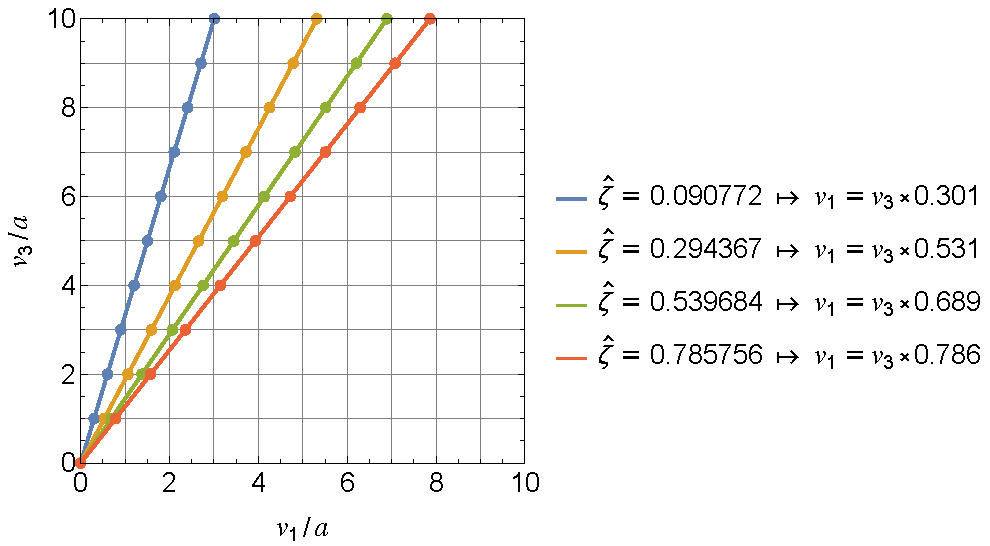
\includegraphics[width=0.5\linewidth]{plots/kinematics_interpolation/v1_v2_allzetahat_plot.pdf}
    \caption{Caption}
    \label{fig:placeholder}
\end{figure}

\pagebreak
\subsubsection{Off-axis \texorpdfstring{$\vect{v}$}{TEXT}}
\begin{figure}[h!]
    \centering
    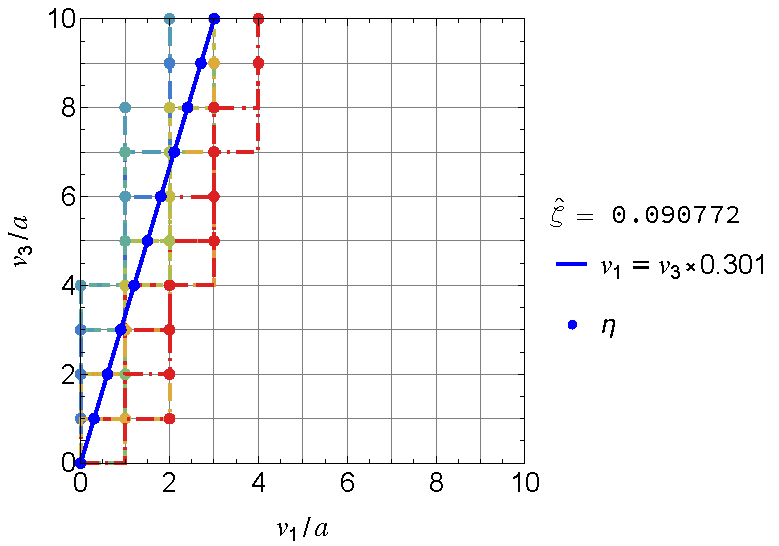
\includegraphics[width=0.5\linewidth]{plots/kinematics_interpolation/v1_v2_withPath_forP-1_plot.pdf}
    \caption{Caption}
    \label{fig:placeholder}
\end{figure}
\begin{figure}[h!]
    \centering
    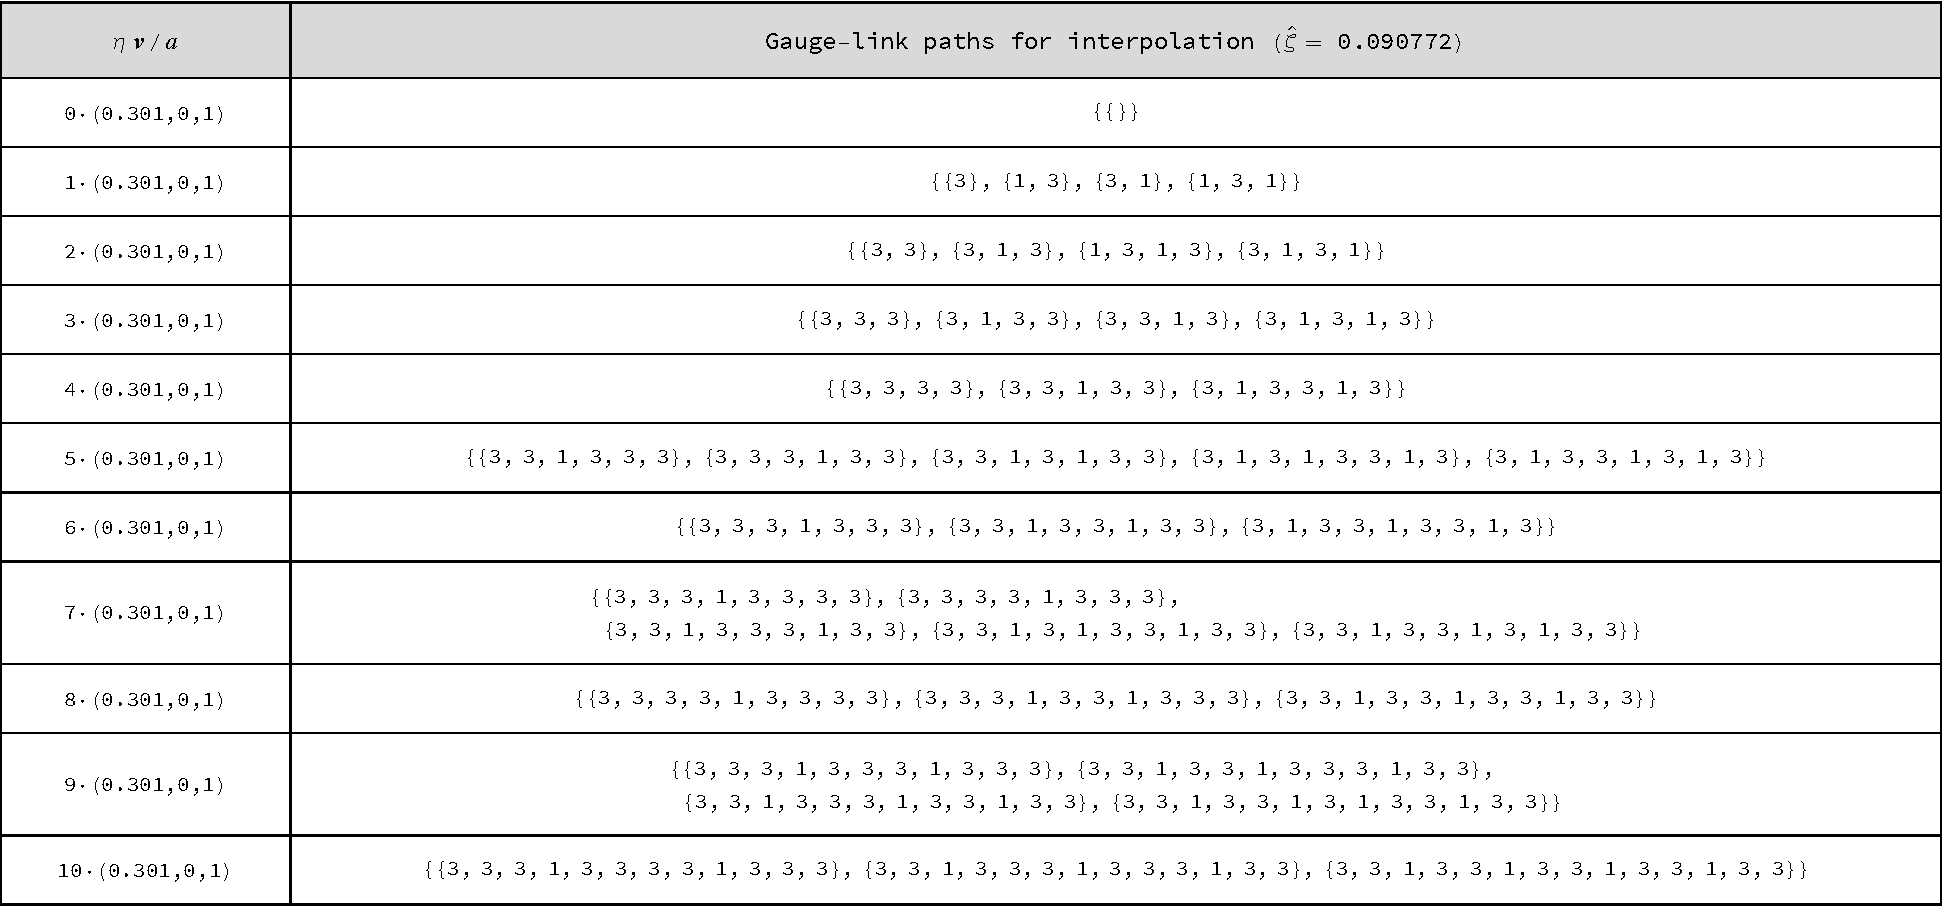
\includegraphics[width=0.8\linewidth]{plots/kinematics_interpolation/eta_gauge_links_forP-1_table.pdf}
    \caption{Caption}
    \label{fig:placeholder}
\end{figure}

\begin{figure}[h!]
    \centering
    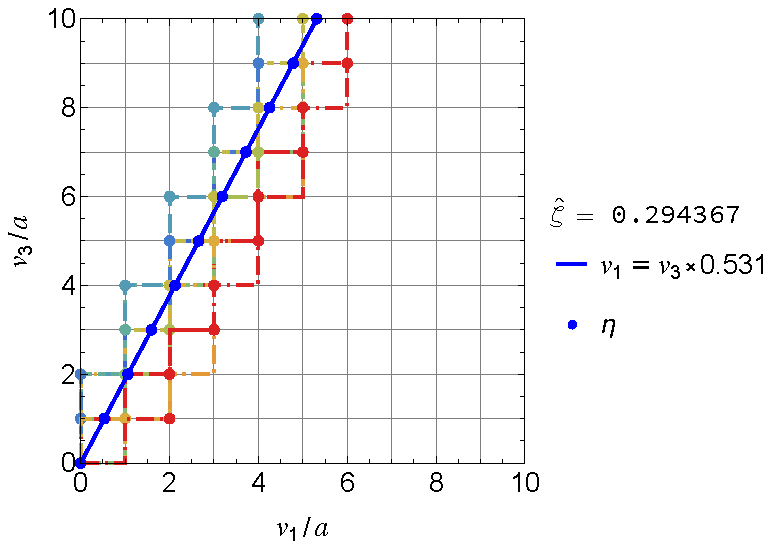
\includegraphics[width=0.5\linewidth]{plots/kinematics_interpolation/v1_v2_withPath_forP-2_plot.pdf}
    \caption{Caption}
    \label{fig:placeholder}
\end{figure}
\begin{figure}[h!]
    \centering
    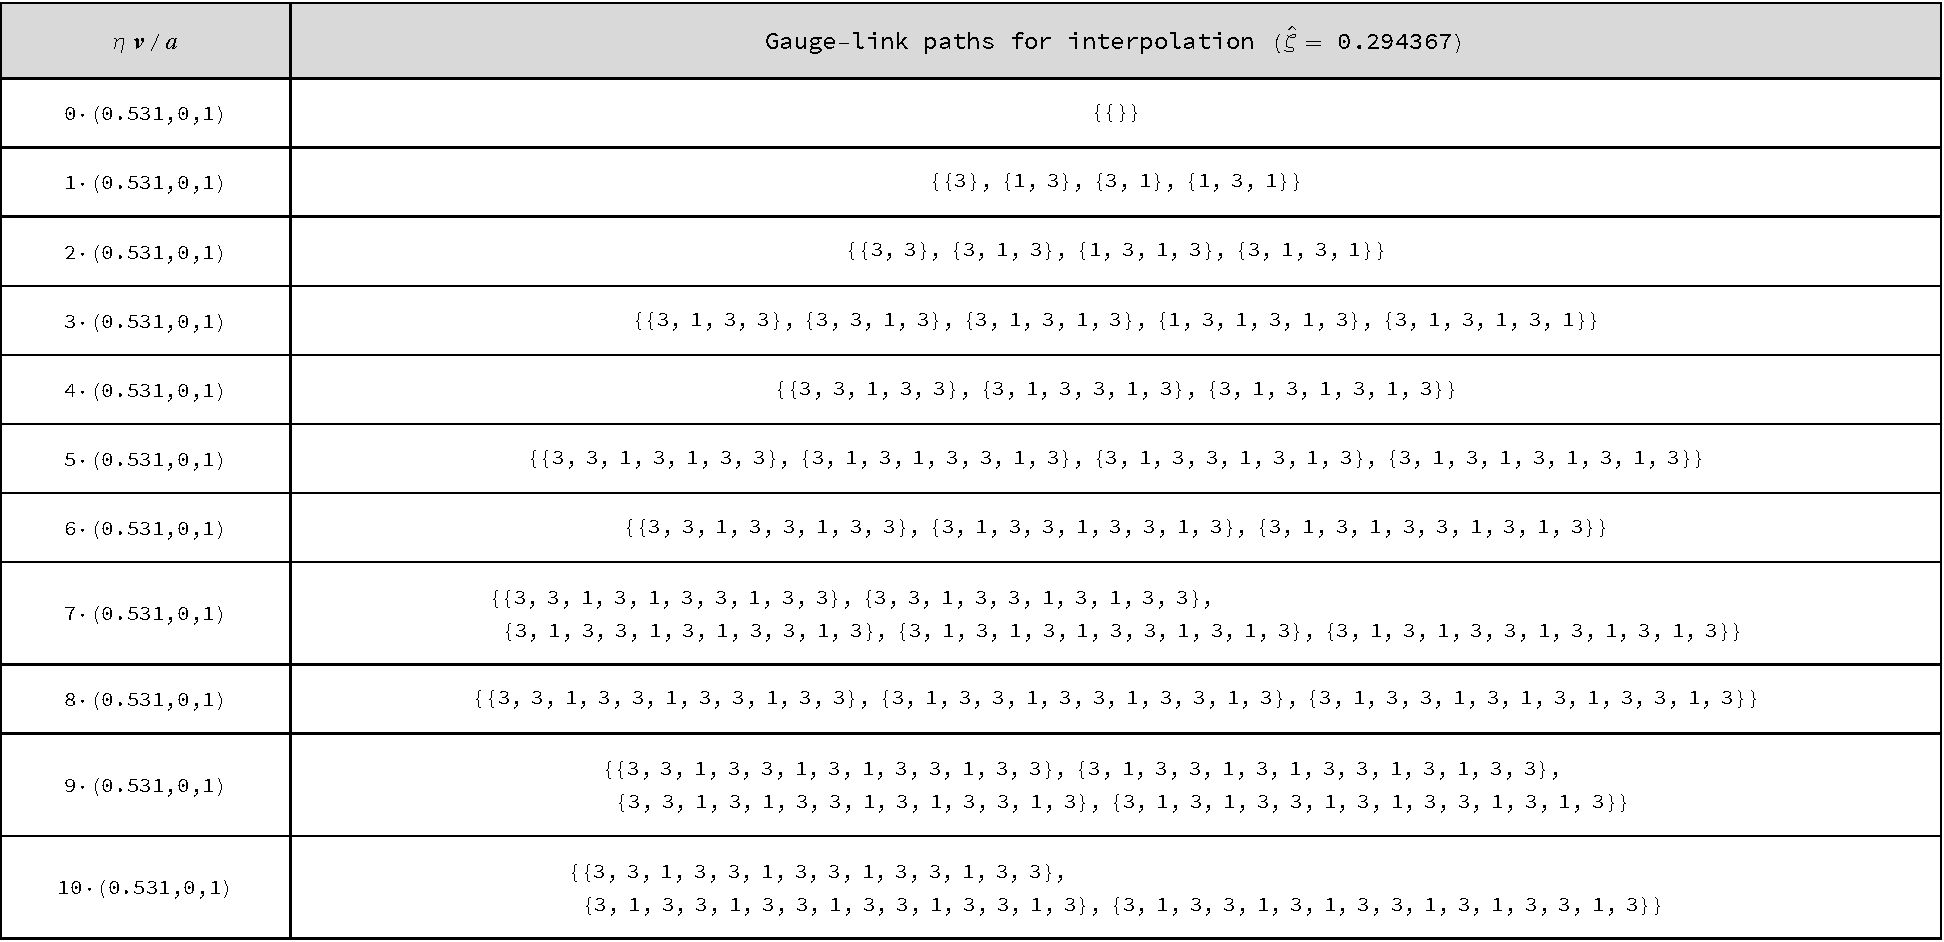
\includegraphics[width=0.8\linewidth]{plots/kinematics_interpolation/eta_gauge_links_forP-2_table.pdf}
    \caption{Caption}
    \label{fig:placeholder}
\end{figure}

\begin{figure}[h!]
    \centering
    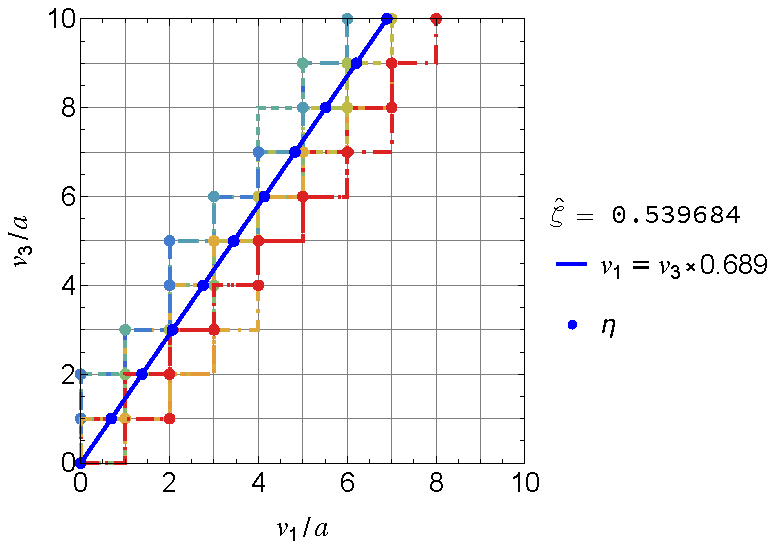
\includegraphics[width=0.5\linewidth]{plots/kinematics_interpolation/v1_v2_withPath_forP-3_plot.pdf}
    \caption{Caption}
    \label{fig:placeholder}
\end{figure}
\begin{figure}[h!]
    \centering
    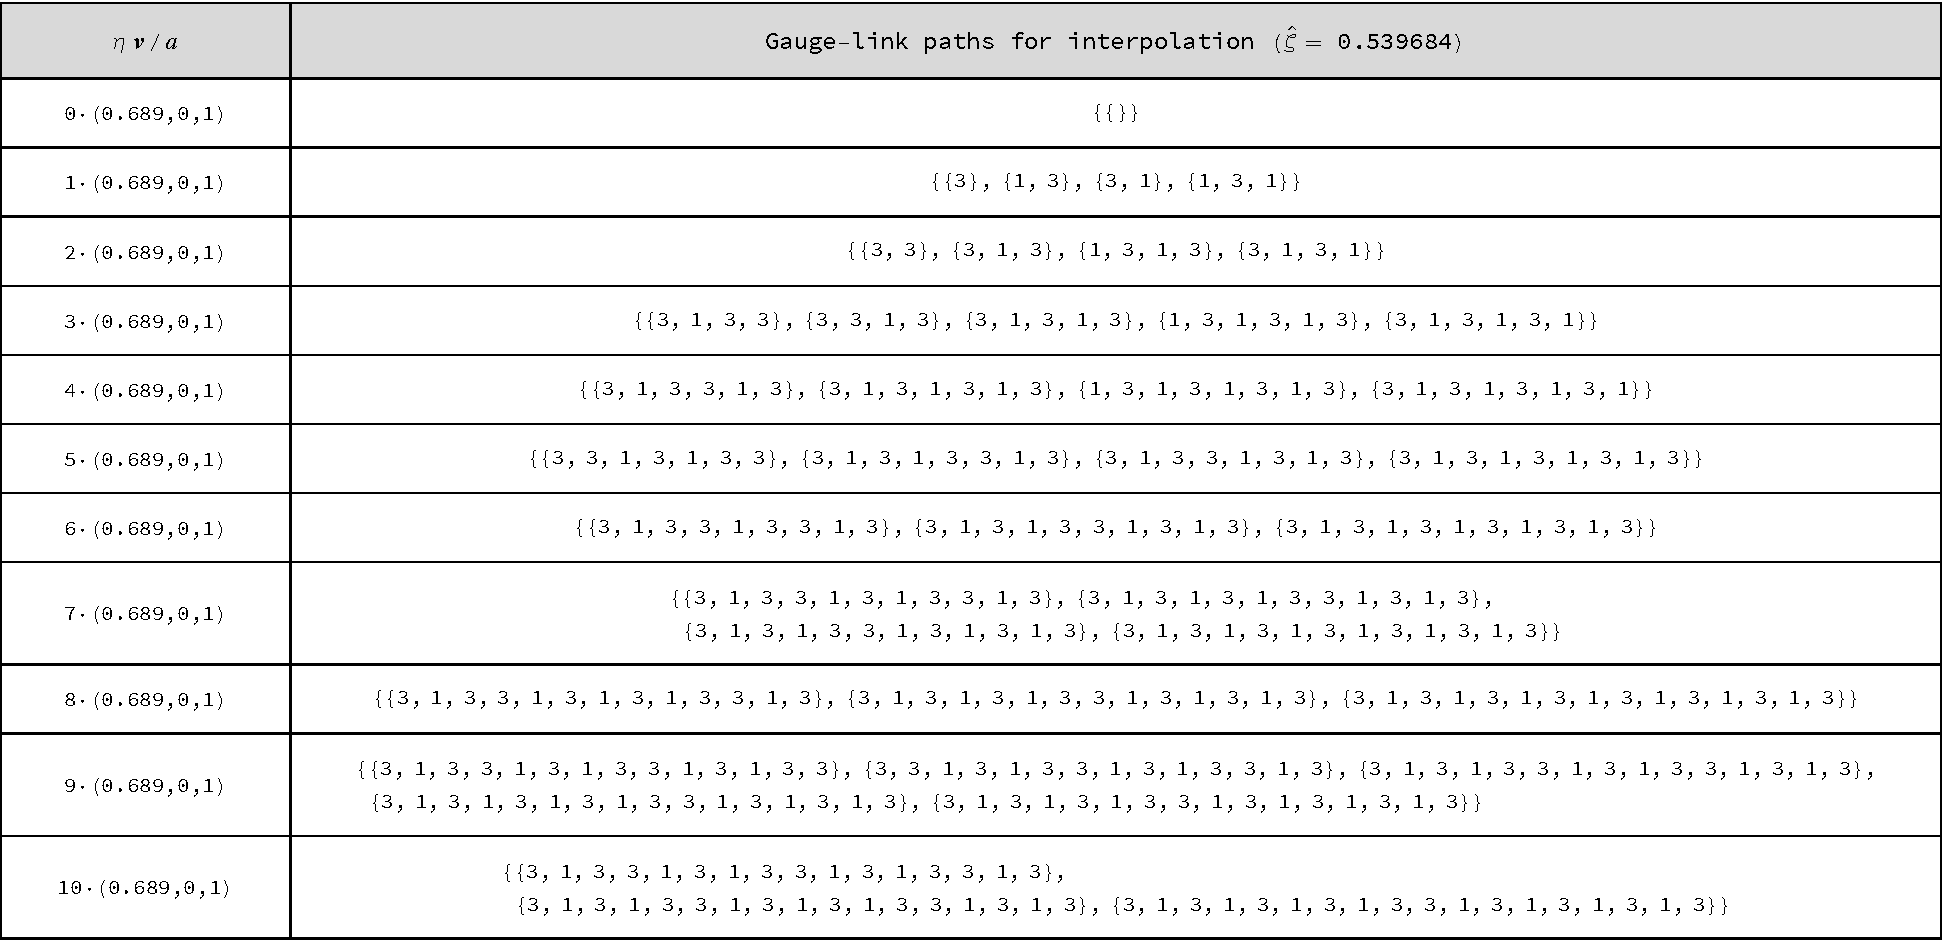
\includegraphics[width=0.8\linewidth]{plots/kinematics_interpolation/eta_gauge_links_forP-3_table.pdf}
    \caption{Caption}
    \label{fig:placeholder}
\end{figure}

\begin{figure}[h!]
    \centering
    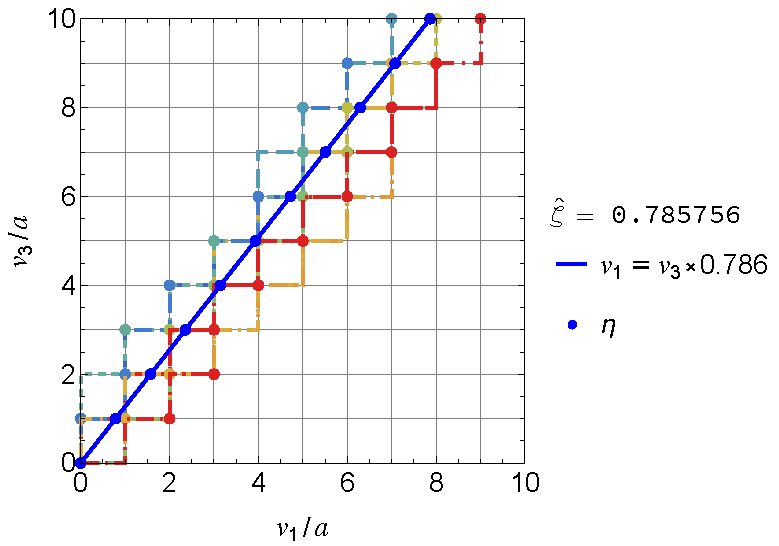
\includegraphics[width=0.5\linewidth]{plots/kinematics_interpolation/v1_v2_withPath_forP-4_plot.pdf}
    \caption{Caption}
    \label{fig:placeholder}
\end{figure}
\begin{figure}[h!]
    \centering
    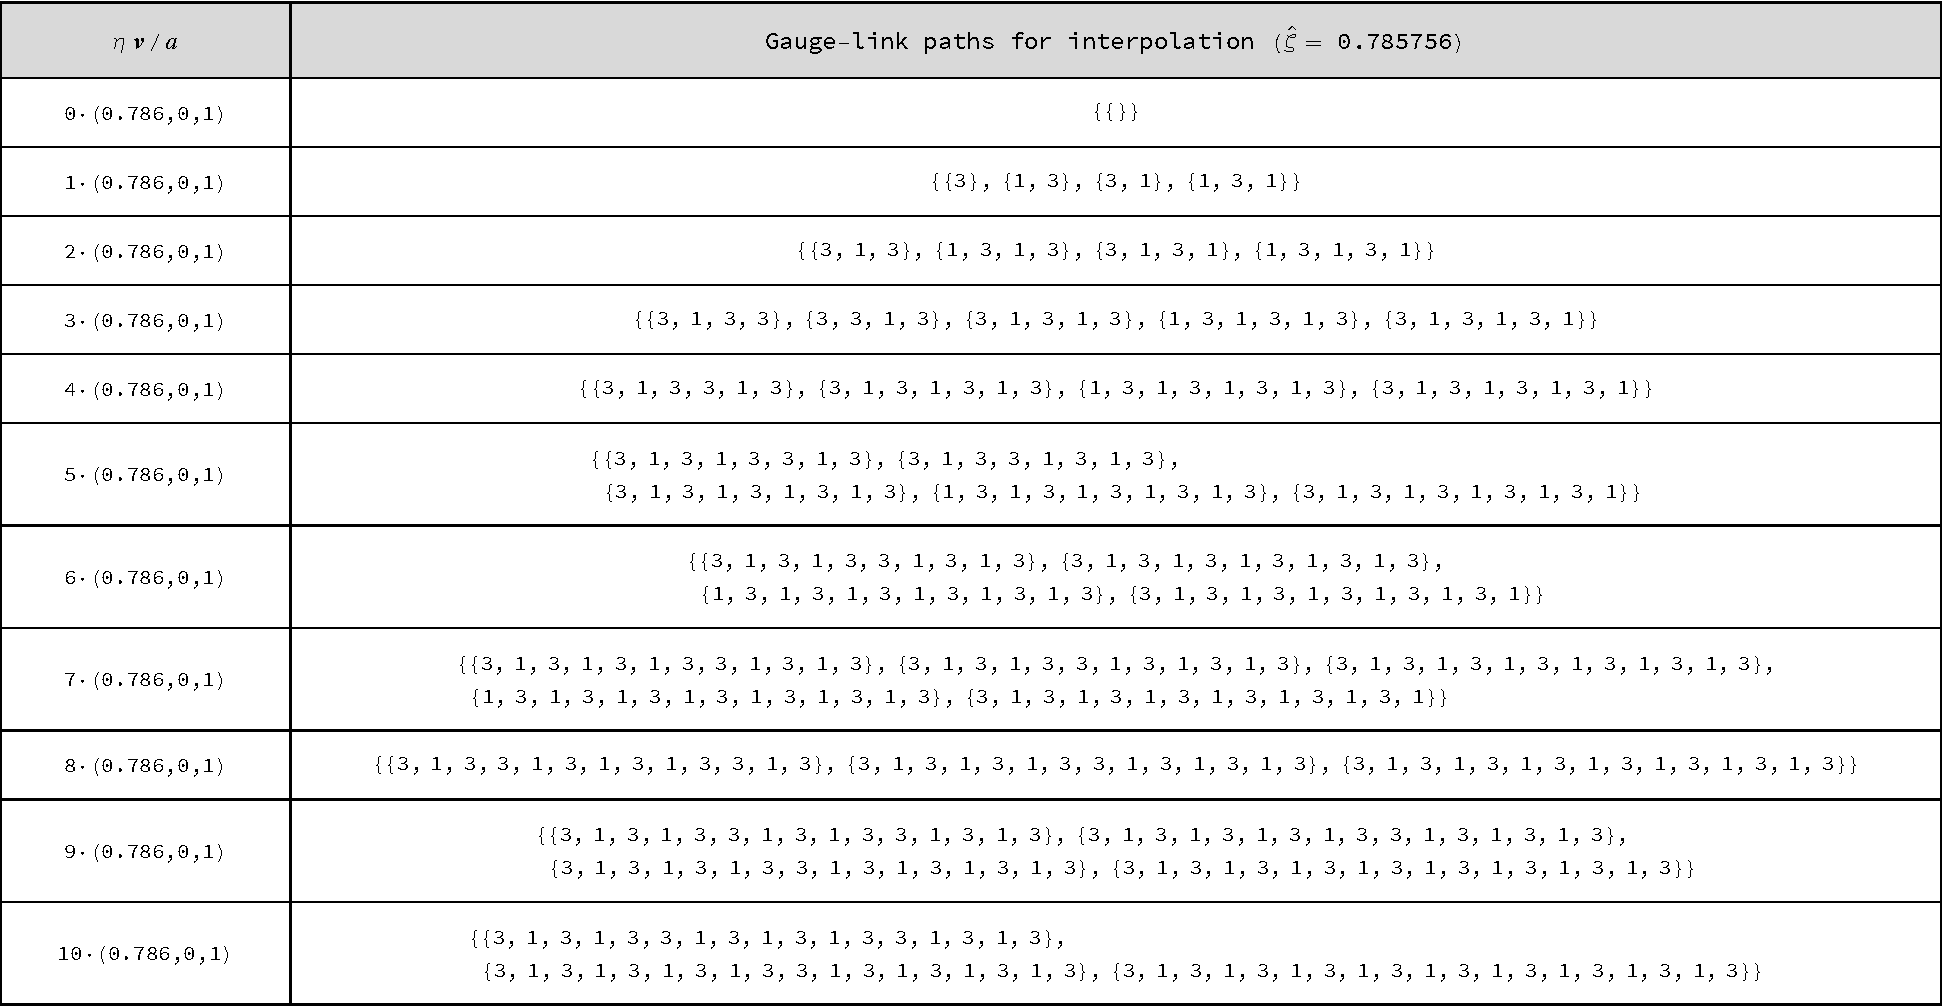
\includegraphics[width=0.8\linewidth]{plots/kinematics_interpolation/eta_gauge_links_forP-4_table.pdf}
    \caption{Caption}
    \label{fig:placeholder}
\end{figure}

\subsection{Deriving \texorpdfstring{$\widetilde \Phi^{[\gamma^+]}$}{TEXT}}
Let's start with the parametrization of the correlator \cite{BMush_Engelhardt2012},
\begin{align}
    \frac{1}{2}\widetilde \Phi^{[\gamma^\mu]}_{\unsub} & = 
		P^\mu\, \tAmp_2 - i \mN^2 \bvec^\mu\, \tAmp_3
		- i \mN \epsilon^{\mu \nu \alpha \beta} P_\nu \bvec_\alpha S_\beta\, \tAmp_{12} \nonumber \\ &
		~~+ \frac{\mN^2}{(v \tcdot P)} v^\mu\, \tBmp_1 
		+ \frac{\mN}{v \tcdot P} \epsilon^{\mu \nu \alpha \beta} P_\nu v_\alpha S_\beta\, \tBmp_7  
		- \frac{ i \mN^3}{v \tcdot P} \epsilon^{\mu \nu \alpha \beta} \bvec_\nu v_\alpha S_\beta\, \tBmp_8 \nonumber \\ &
		~~- \frac{\mN^3}{v \tcdot P} (\bvec \tcdot S) \epsilon^{\mu \nu \alpha \beta} P_\nu \bvec_\alpha v_\beta\, \tBmp_9
		- \frac{i \mN^3}{(v \tcdot P)^2} (v \tcdot S) \epsilon^{\mu \nu \alpha \beta} P_\nu \bvec_\alpha v_\beta \tBmp_{10}
\end{align}
 For the lattice calculations, it is, however, advantageous to start with an equivalent parametrization in which the structures explicitly depend on the staple extent $\eta$ and which is still well-defined for $ v\cdot P = 0$. Such a parametrization can be obtained from the parametrization above by replacing $v \rightarrow \eta v$ and by leaving out the factors $(v \tcdot P)^{-n}$. 
 \begin{align}
    \frac{1}{2}\widetilde \Phi^{[\gamma^\mu]}_{\unsub}=\frac{1}{2} R_{\gamma^{\mu}} E_N & =  
		P^\mu\, \tilde a_2 - i \mN^2 \bvec^\mu\, \tilde a_3
		- i \mN \epsilon^{\mu \nu \alpha \beta} P_\nu \bvec_\alpha S_\beta\, \tilde a_{12} \nonumber \\ &
		~~+ \mN^2 \eta v^\mu\, \tilde b_1 
		+ \mN \epsilon^{\mu \nu \alpha \beta} P_\nu \eta v_\alpha S_\beta\, \tilde b_7  
		-  i \mN^3 \epsilon^{\mu \nu \alpha \beta} \bvec_\nu \eta v_\alpha S_\beta\, \tilde b_8 \nonumber \\ &
		~~- \mN^3 (\bvec \tcdot S) \epsilon^{\mu \nu \alpha \beta} P_\nu \bvec_\alpha \eta v_\beta\, \tilde b_9
		-i \mN^3 (v \tcdot S) \epsilon^{\mu \nu \alpha \beta} P_\nu \bvec_\alpha \eta^2 v_\beta \tilde b_{10}
\end{align}
For $P^{\mu}=(E_N, -|\vec{P}^1|,0,0)$, $b^{\mu}=(0,b_{1},b_{2},0)$, $v^{\mu}=\pm n^{\prime}(0,v_{1},0,v_{3})$, $S^{\mu}=(0,0,0,1)$,
\begin{align}
    \frac{1}{2}\widetilde \Phi^{[\gamma^{0}]}_{\unsub} & = 
		P^0\, \tAmp_2 - \cancelto{0}{i \mN^2 \bvec^0\, \tAmp_3}
		+ i \mN \underbrace{\epsilon^{0 123}}_{1} |\vec{P}^1| \bvec_2 S_3\, \tAmp_{12} \nonumber \\ &
		~~+ \cancelto{0}{\frac{\mN^2}{(v \tcdot P)} v^0\, \tBmp_1 }
		+ \cancelto{0}{\frac{\mN}{v \tcdot P} \epsilon^{0 113} P_1 v_1 S_3\, \tBmp_7  }+ \cancelto{0}{\frac{\mN}{v \tcdot P} \epsilon^{0 133} P_1 v_3 S_3\, \tBmp_7  }
		 \nonumber \\ &
		~~- \frac{ i \mN^3}{v \tcdot P} \underbrace{\epsilon^{0 213}}_{-1} \bvec_2 v_1 S_3\, \tBmp_8 - \cancelto{0}{\frac{ i \mN^3}{v \tcdot P}\epsilon^{0 113} \bvec_1 v_1 S_3\, \tBmp_8}- \cancelto{0}{\frac{ i \mN^3}{v \tcdot P}\epsilon^{0 133} \bvec_1 v_3 S_3\, \tBmp_8}- \cancelto{0}{\frac{ i \mN^3}{v \tcdot P}\epsilon^{0 233} \bvec_2 v_3 S_3\, \tBmp_8}\nonumber \\ &
		~~+ \frac{\mN^3}{v \tcdot P} \cancelto{0}{(\bvec \tcdot S)} \underbrace{\epsilon^{0 123}}_{1} |\vec{P}_1| \bvec_2 v_3\, \tBmp_9- \cancelto{0}{\frac{\mN^3}{v \tcdot P} (\bvec \tcdot S) \epsilon^{0 121} P_1 \bvec_2 v_1\, \tBmp_9}- \cancelto{0}{\frac{\mN^3}{v \tcdot P} (\bvec \tcdot S) \epsilon^{0 113} P_1 \bvec_1 v_3\, \tBmp_9}- \cancelto{0}{\frac{\mN^3}{v \tcdot P} (\bvec \tcdot S) \epsilon^{0 111} P_1 \bvec_1 v_1\, \tBmp_9}\nonumber \\ &
		~~+ \frac{i \mN^3}{(v \tcdot P)^2} (v \tcdot S) \underbrace{\epsilon^{0 123}}_{1} |\vec{P}_1| \bvec_2 v_3 \tBmp_{10}
		- \cancelto{0}{\frac{i \mN^3}{(v \tcdot P)^2} (v \tcdot S) \epsilon^{0 121} P_1 \bvec_2 v_1 \tBmp_{10}}- \cancelto{0}{\frac{i \mN^3}{(v \tcdot P)^2} (v \tcdot S) \epsilon^{0 111} P_1 \bvec_1 v_1 \tBmp_{10}}\nonumber \\ &
		~~- \cancelto{0}{\frac{i \mN^3}{(v \tcdot P)^2} (v \tcdot S) \epsilon^{0 113} P_1 \bvec_1 v_3 \tBmp_{10}}\\
  \Aboxed{ \frac{1}{2}\widetilde \Phi^{[\gamma^{0}]}_{\unsub}& = P^0\, \tAmp_2  + i \mN  |\vec{P}^1| \bvec_2 S_3\, \tAmp_{12}+ \frac{ i \mN^3}{v \tcdot P}  \bvec_2 v_1 S_3\, \tBmp_8+ \frac{i \mN^3}{(v \tcdot P)^2} (v \tcdot S)  |P_1| \bvec_2 v_3 \tBmp_{10}}
\end{align}
and
\begin{align}
    \frac{1}{2}\widetilde \Phi^{[\gamma^{1}]}_{\unsub} & = 
		-|\vec{P}^1|\, \tAmp_2 - i \mN^2 \bvec^1\, \tAmp_3
		- i \mN \underbrace{\epsilon^{1 023}}_{-1} P_0 \bvec_2 S_3\, \tAmp_{12} \nonumber \\ &
		~~+ \frac{\mN^2}{(v \tcdot P)} v^1\, \tBmp_1 
		+ \cancelto{0}{\frac{\mN}{v \tcdot P} \epsilon^{1 013} P_0 v_1 S_3\, \tBmp_7  }+ \cancelto{0}{\frac{\mN}{v \tcdot P} \epsilon^{1 033} P_0 v_3 S_3\, \tBmp_7  }
		- \cancelto{0}{\frac{ i \mN^3}{v \tcdot P} \epsilon^{1 213} \bvec_2 v_1 S_3\, \tBmp_8}- \cancelto{0}{\frac{ i \mN^3}{v \tcdot P} \epsilon^{1 233} \bvec_2 v_3 S_3\, \tBmp_8} \nonumber \\ &
  ~~- \cancelto{0}{\frac{ i \mN^3}{v \tcdot P} \epsilon^{1 133} \bvec_1 v_3 S_3\, \tBmp_8}- \cancelto{0}{\frac{ i \mN^3}{v \tcdot P} \epsilon^{1 113} \bvec_1 v_1 S_3\, \tBmp_8}- \frac{\mN^3}{v \tcdot P} \cancelto{0}{(\bvec \tcdot S)} \underbrace{\epsilon^{1 023}}_{1} P_0 \bvec_2 v_3\, \tBmp_9- \cancelto{0}{\frac{\mN^3}{v \tcdot P} (\bvec \tcdot S) \epsilon^{1 021} P_0 \bvec_2 v_1\, \tBmp_9} \nonumber \\ &
		~~
		- \frac{i \mN^3}{(v \tcdot P)^2} (v \tcdot S) \underbrace{\epsilon^{1 023}}_{-1} P_0 \bvec_2 v_3 \tBmp_{10}- \cancelto{0}{\frac{i \mN^3}{(v \tcdot P)^2} (v \tcdot S) \epsilon^{1 021} P_0 \bvec_2 v_1 \tBmp_{10}}\\
  \Aboxed{ \frac{1}{2}\widetilde \Phi^{[\gamma^{1}]}_{\unsub} & =-|\vec{P}^1|\, \tAmp_2+ \frac{\mN^2}{(v \tcdot P)} v^1\, \tBmp_1 
		+ i \mN  P_0 \bvec_2 S_3\, \tAmp_{12}+ \frac{i \mN^3}{(v \tcdot P)^2} (v \tcdot S)  P_0 \bvec_2 v_3 \tBmp_{10}- i \mN^2 \bvec^1\, \tAmp_3}
\end{align}
for $\mu=2$
\begin{align}
    \frac{1}{2}\widetilde \Phi^{[\gamma^2]}_{\unsub} & = 
		 - i \mN^2 \bvec^2\, \tAmp_3
		- i \mN \underbrace{\epsilon^{2 0 1 3}}_{1} P_0 \bvec_1 S_3\, \tAmp_{12} \nonumber \\ &
		~~
		+ \frac{\mN}{v \tcdot P} \underbrace{\epsilon^{2 0 1 3}}_{1} P_0 v_1 S_3\, \tBmp_7  
		 \nonumber \\ &
		~~
		- \frac{i \mN^3}{(v \tcdot P)^2} (v \tcdot S) \underbrace{\epsilon^{2 0 1 3}}_{1} P_0 \bvec_1 v_3 \tBmp_{10}\\
  \Aboxed{\frac{1}{2}\widetilde \Phi^{[\gamma^2]}_{\unsub} & =- i \mN^2 \bvec^2\, \tAmp_3
		- i \mN  P_0 \bvec_1 S_3\, \tAmp_{12}+ \frac{\mN}{v \tcdot P}  P_0 v_1 S_3\, \tBmp_7- \frac{i \mN^3}{(v \tcdot P)^2} (v \tcdot S) P_0 \bvec_1 v_3 \tBmp_{10}}
\end{align}
for $\mu=3$
\begin{align}
    \frac{1}{2}\widetilde \Phi^{[\gamma^3]}_{\unsub} & = \frac{\mN^2}{(v \tcdot P)} v^3\, \tBmp_1 
		\nonumber \\ &
		~~
		- \frac{i \mN^3}{(v \tcdot P)^2} (v \tcdot S) \underbrace{\epsilon^{3 0 2 1}}_{1} P_0 \bvec_2 v_1 \tBmp_{10}\\
  \Aboxed{\frac{1}{2}\widetilde \Phi^{[\gamma^3]}_{\unsub}& = \frac{\mN^2}{(v \tcdot P)} v^3\, \tBmp_1- \frac{i \mN^3}{(v \tcdot P)^2} (v \tcdot S)  P_0 \bvec_2 v_1 \tBmp_{10}}
\end{align}
So, we have
\begin{align}
   \Aboxed{ \frac{1}{2}\widetilde \Phi^{[\gamma^{0}]}_{\unsub}& = P^0\, \tAmp_2  + i \mN  |\vec{P}^1| \bvec_2 S_3\, \tAmp_{12}+ \frac{ i \mN^3}{v \tcdot P}  \bvec_2 v_1 S_3\, \tBmp_8+ \frac{i \mN^3}{(v \tcdot P)^2} (v \tcdot S)  |P_1| \bvec_2 v_3 \tBmp_{10}}\\
   \Aboxed{ \frac{1}{2}\widetilde \Phi^{[\gamma^{1}]}_{\unsub} & =-|\vec{P}^1|\, \tAmp_2- i \mN^2 \bvec^1\, \tAmp_3+ \frac{\mN^2}{(v \tcdot P)} v^1\, \tBmp_1 
		+ i \mN  P_0 \bvec_2 S_3\, \tAmp_{12}+ \frac{i \mN^3}{(v \tcdot P)^2} (v \tcdot S)  P_0 \bvec_2 v_3 \tBmp_{10}}\\
   \Aboxed{\frac{1}{2}\widetilde \Phi^{[\gamma^2]}_{\unsub} & =- i \mN^2 \bvec^2\, \tAmp_3
		- i \mN  P_0 \bvec_1 S_3\, \tAmp_{12}+ \frac{\mN}{v \tcdot P}  P_0 v_1 S_3\, \tBmp_7- \frac{i \mN^3}{(v \tcdot P)^2} (v \tcdot S) P_0 \bvec_1 v_3 \tBmp_{10}}\\
    \Aboxed{\frac{1}{2}\widetilde \Phi^{[\gamma^3]}_{\unsub}& = \frac{\mN^2}{(v \tcdot P)} v^3\, \tBmp_1- \frac{i \mN^3}{(v \tcdot P)^2} (v \tcdot S)  P_0 \bvec_2 v_1 \tBmp_{10}}
\end{align}
\begin{align}
    \begin{pmatrix}
        \rule{0pt}{16pt} \widetilde \Phi^{[\gamma^{0}]}_{\unsub}\\
        \rule{0pt}{16pt} \widetilde \Phi^{[\gamma^{1}]}_{\unsub}\\
        \rule{0pt}{16pt} \widetilde \Phi^{[\gamma^{2}]}_{\unsub}\\
        \rule{0pt}{16pt} \widetilde \Phi^{[\gamma^{3}]}_{\unsub}
    \end{pmatrix} &=2\begin{pmatrix}
       \rule{0pt}{16pt}  P^0\, \tAmp_2  + i \mN  |\vec{P}^1| \bvec_2 S_3\, \tAmp_{12}+ \frac{ i \mN^3}{v \tcdot P}  \bvec_2 v_1 S_3\, \tBmp_8+ \frac{i \mN^3}{(v \tcdot P)^2} (v \tcdot S)  |P_1| \bvec_2 v_3 \tBmp_{10}\\
        \rule{0pt}{16pt} -|\vec{P}^1|\, \tAmp_2- i \mN^2 \bvec^1\, \tAmp_3+ \frac{\mN^2}{(v \tcdot P)} v^1\, \tBmp_1 
		+ i \mN  P_0 \bvec_2 S_3\, \tAmp_{12}+ \frac{i \mN^3}{(v \tcdot P)^2} (v \tcdot S)  P_0 \bvec_2 v_3 \tBmp_{10}\\
         \rule{0pt}{16pt} - i \mN^2 \bvec^2\, \tAmp_3
		- i \mN  P_0 \bvec_1 S_3\, \tAmp_{12}+ \frac{\mN}{v \tcdot P}  P_0 v_1 S_3\, \tBmp_7- \frac{i \mN^3}{(v \tcdot P)^2} (v \tcdot S) P_0 \bvec_1 v_3 \tBmp_{10}\\
        \rule{0pt}{16pt} \frac{\mN^2}{(v \tcdot P)} v^3\, \tBmp_1- \frac{i \mN^3}{(v \tcdot P)^2} (v \tcdot S)  P_0 \bvec_2 v_1 \tBmp_{10}
    \end{pmatrix}
\end{align}
let's write everything in upper index form,
\begin{align}
    \begin{pmatrix}
        \rule{0pt}{16pt} \widetilde \Phi^{[\gamma^{0}]}_{\unsub}\\
        \rule{0pt}{16pt} \widetilde \Phi^{[\gamma^{1}]}_{\unsub}\\
        \rule{0pt}{16pt} \widetilde \Phi^{[\gamma^{2}]}_{\unsub}\\
        \rule{0pt}{16pt} \widetilde \Phi^{[\gamma^{3}]}_{\unsub}
    \end{pmatrix} &=2\begin{pmatrix}
       \rule{0pt}{16pt}  P^0\, \tAmp_2  - i \mN  |\vec{P}^1| \bvec^2 S^3\, \tAmp_{12}- \frac{ i \mN^3}{v \tcdot P}  \bvec^2 v^1 S^3\, \tBmp_8- \frac{i \mN^3}{(v \tcdot P)^2} (v \tcdot S)  |\vec{P}^1| \bvec^2 v^3 \tBmp_{10}\\
        \rule{0pt}{16pt} -|\vec{P}^1|\, \tAmp_2- i \mN^2 \bvec^1\, \tAmp_3+ \frac{\mN^2}{(v \tcdot P)} v^1\, \tBmp_1 
		+ i \mN  P^0 \bvec^2 S^3\, \tAmp_{12}+ \frac{i \mN^3}{(v \tcdot P)^2} (v \tcdot S)  P^0 \bvec^2 v^3 \tBmp_{10}\\
         \rule{0pt}{16pt} - i \mN^2 \bvec^2\, \tAmp_3
		- i \mN  P^0 \bvec^1 S^3\, \tAmp_{12}+ \frac{\mN}{v \tcdot P}  P^0 v^1 S^3\, \tBmp_7- \frac{i \mN^3}{(v \tcdot P)^2} (v \tcdot S) P^0 \bvec^1 v^3 \tBmp_{10}\\
        \rule{0pt}{16pt} \frac{\mN^2}{(v \tcdot P)} v^3\, \tBmp_1- \frac{i \mN^3}{(v \tcdot P)^2} (v \tcdot S)  P^0 \bvec^2 v^1 \tBmp_{10}
    \end{pmatrix}
\end{align}

The relation to the upper-case amplitudes is given by
\begin{align}
	\tAmp_i\left(\bvec^2,\bvec \tcdot P,\frac{v \tcdot \bvec}{v \tcdot P}, \frac{v^2}{(v \tcdot P)^2}, \eta v \tcdot P\right) & = \tilde a_i(\bvec^2,\bvec \tcdot P, \eta v \tcdot b, (\eta v)^2, \eta v \tcdot P)    \, , \nonumber \\
	 \tBmp_i\left(\bvec^2,\bvec \tcdot P,\frac{v \tcdot \bvec}{v \tcdot P}, \frac{v^2}{(v \tcdot P)^2}, \eta v \tcdot P\right) & = (\eta v \tcdot P)^n\ \tilde b_i(\bvec^2,\bvec \tcdot P, \eta v \tcdot b, (\eta v)^2, \eta v \tcdot P)   \, ,
	\label{eq-ab}
\end{align}
In general, the amplitudes are complex,
\begin{align}
    \tilde{a}_i&=\tilde{a}^{\text{Re}}_i+i\tilde{a}^{\text{Im}}_i\\
    \tilde{b}_i&=\tilde{b}^{\text{Re}}_i+i\tilde{b}^{\text{Im}}_i
\end{align}
then
\begin{align}
    \begin{pmatrix}
        \rule{0pt}{16pt} R_{\Gamma(1)}\\
        \rule{0pt}{16pt} R_{\Gamma(2)}\\
        \rule{0pt}{16pt} R_{\Gamma(4)}\\
        \rule{0pt}{16pt} R_{\Gamma(8)}
    \end{pmatrix} = \begin{pmatrix}
        \rule{0pt}{16pt} R_{[+i\gamma^1]}\\
        \rule{0pt}{16pt} R_{[-i\gamma^2]}\\
        \rule{0pt}{16pt} R_{[+i\gamma^3]}\\
        \rule{0pt}{16pt} R_{[\gamma^0]}
    \end{pmatrix} &=2\begin{pmatrix}
        \rule{0pt}{16pt} -i\frac{|\vec{P}^1|}{E_N}\, \tilde a_2+  \frac{\mN^2}{E_N} \bvec^1\, \tilde a_3+ i\frac{\mN^2}{E_N} \eta v^1\, \tilde b_1 
		-  \mN  \bvec^2 \, \tilde a_{12}+  \mN^3  \bvec^2 \eta^2 (v^3)^2 \tilde b_{10}\\
         \rule{0pt}{16pt} -  \frac{\mN^2}{E_N} \bvec^2\, \tilde a_3
		-  \mN   \bvec^1  \tilde a_{12}-i \mN \eta  v^1  \tilde b_7+ \mN^3  \bvec^1 \eta^2 (v^3)^2 \tilde b_{10}\\
        \rule{0pt}{16pt} i\frac{\mN^2}{E_N} \eta v^3\, \tilde b_1-  \mN^3 \bvec^2 \eta^2 v^1 v^3\tilde b_{10}\\
         \rule{0pt}{16pt}   \tilde a_2  - i \mN  \frac{|\vec{P}^1|}{E_N} \bvec^2  \tilde a_{12}- \frac{ i \mN^3}{E_N}  \bvec^2 \eta v^1  \tilde b_8+ \frac{i \mN^3}{E_N}  |\vec{P}^1| \bvec^2 \eta^2 (v^3)^2 \tilde b_{10}
    \end{pmatrix}
\end{align}
On making two set of equations by flipping only the $b^1=b_{L}$, for positive $b^1$, we have 
%
\begin{align}
    \begin{pmatrix}
        \rule{0pt}{16pt} \text{Re}\{ R_{\Gamma(1)}\}^{[+b^1]} \\
        \rule{0pt}{16pt} \text{Im}\{ R_{\Gamma(1)}\}^{[+b^1]} \\
        \rule{0pt}{16pt} \text{Re}\{ R_{\Gamma(2)}\}^{[+b^1]} \\
        \rule{0pt}{16pt} \text{Im}\{ R_{\Gamma(2)}\}^{[+b^1]} \\
        \rule{0pt}{16pt} \text{Re}\{ R_{\Gamma(4)}\}^{[+b^1]} \\
        \rule{0pt}{16pt} \text{Im}\{ R_{\Gamma(4)}\}^{[+b^1]} \\
        \rule{0pt}{16pt} \text{Re}\{ R_{\Gamma(8)}\}^{[+b^1]} \\
        \rule{0pt}{16pt} \text{Im}\{ R_{\Gamma(8)}\}^{[+b^1]}
    \end{pmatrix} &= 2\begin{pmatrix}
     \rule{0pt}{16pt}   \frac{\mN^2}{E_N} \bvec^1\, \tilde a^{\text{Re}}_3-  \mN  \bvec^2 \, \tilde a^{\text{Re}}_{12}+  \mN^3  \bvec^2 \eta^2 (v^3)^2 \tilde b^{\text{Re}}_{10} +\frac{|\vec{P}^1|}{E_N}\, \tilde a^{\text{Im}}_2- \frac{\mN^2}{E_N} \eta v^1\, \tilde b^{\text{Im}}_1\\
      \rule{0pt}{16pt}  -\frac{|\vec{P}^1|}{E_N}\, \tilde a^{\text{Re}}_2+ \frac{\mN^2}{E_N} \eta v^1\, \tilde b^{\text{Re}}_1 + \frac{\mN^2}{E_N} \bvec^1\, \tilde a^{\text{Im}}_3-  \mN  \bvec^2 \, \tilde a^{\text{Im}}_{12}+  \mN^3  \bvec^2 \eta^2 (v^3)^2 \tilde b^{\text{Im}}_{10}\\
      \rule{0pt}{16pt}  -  \frac{\mN^2}{E_N} \bvec^2\, \tilde a^{\text{Re}}_3
		-  \mN   \bvec^1  \tilde a^{\text{Re}}_{12}+ \mN^3  \bvec^1 \eta^2 (v^3)^2 \tilde b^{\text{Re}}_{10}+\mN \eta v^1  \tilde b^{\text{Im}}_7 \\
      \rule{0pt}{16pt} - \mN \eta v^1  \tilde b^{\text{Re}}_7 -  \frac{\mN^2}{E_N} \bvec^2\, \tilde a^{\text{Im}}_3
		-  \mN   \bvec^1  \tilde a^{\text{Im}}_{12}+ \mN^3  \bvec^1 \eta^2 (v^3)^2 \tilde b^{\text{Im}}_{10}\\
      \rule{0pt}{16pt} -\mN^3 \bvec^2 \eta^2 v^1 v^3\tilde b^{\text{Re}}_{10}-\frac{\mN^2}{E_N} \eta v^3\, \tilde b^{\text{Im}}_1\\
      \rule{0pt}{16pt} \frac{\mN^2}{E_N} \eta v^3\, \tilde b^{\text{Re}}_1 -\mN^3 \bvec^2 \eta^2 v^1 v^3\tilde b^{\text{Im}}_{10}\\
      \rule{0pt}{16pt}  \tilde a^{\text{Re}}_2 +  \mN  \frac{|\vec{P}^1|}{E_N} \bvec^2  \tilde a^{\text{Im}}_{12}+ \frac{  \mN^3}{E_N}  \bvec^2 \eta v^1  \tilde b^{\text{Im}}_8- \frac{ \mN^3}{E_N}  |\vec{P}^1| \bvec^2 \eta^2 (v^3)^2 \tilde b^{\text{Im}}_{10}\\
      \rule{0pt}{16pt} -  \mN  \frac{|\vec{P}^1|}{E_N} \bvec^2  \tilde a^{\text{Re}}_{12}- \frac{  \mN^3}{E_N}  \bvec^2 \eta v^1  \tilde b^{\text{Re}}_8+ \frac{ \mN^3}{E_N}  |\vec{P}^1| \bvec^2 \eta^2 (v^3)^2 \tilde b^{\text{Re}}_{10}+\tilde a^{\text{Im}}_2
    \end{pmatrix}
\end{align}
and for negative $b^1$, by construction $\tilde{A}^{\text{Im}}_i=\tilde{A}^{\text{(b-odd})}_i=\tilde{A}^{\text{($b^1$-odd})}_i$ and  $\tilde{B}^{\text{Im}}_i=\tilde{B}^{\text{(b-odd})}_i=\tilde{B}^{\text{($b^1$-odd})}_i$ we have 
\begin{align}
    \begin{pmatrix}
        \rule{0pt}{16pt} \text{Re}\{ R_{\Gamma(1)}\}^{[-b^1]} \\
        \rule{0pt}{16pt} \text{Im}\{ R_{\Gamma(1)}\}^{[-b^1]} \\
        \rule{0pt}{16pt} \text{Re}\{ R_{\Gamma(2)}\}^{[-b^1]} \\
        \rule{0pt}{16pt} \text{Im}\{ R_{\Gamma(2)}\}^{[-b^1]} \\
        \rule{0pt}{16pt} \text{Re}\{ R_{\Gamma(4)}\}^{[-b^1]} \\
        \rule{0pt}{16pt} \text{Im}\{ R_{\Gamma(4)}\}^{[-b^1]} \\
        \rule{0pt}{16pt} \text{Re}\{ R_{\Gamma(8)}\}^{[-b^1]} \\
        \rule{0pt}{16pt} \text{Im}\{ R_{\Gamma(8)}\}^{[-b^1]}
    \end{pmatrix} &= 2\begin{pmatrix}
     \rule{0pt}{16pt}   \textcolor{red}{-}\frac{\mN^2}{E_N} \bvec^1\, \tilde a^{\text{Re}}_3-  \mN  \bvec^2 \, \tilde a^{\text{Re}}_{12}+  \mN^3  \bvec^2 \eta^2 (v^3)^2 \tilde b^{\text{Re}}_{10} \textcolor{red}{-}\frac{|\vec{P}^1|}{E_N}\, \tilde a^{\text{Im}}_2\textcolor{red}{+} \frac{\mN^2}{E_N} \eta v^1\, \tilde b^{\text{Im}}_1\\
      \rule{0pt}{16pt}  -\frac{|\vec{P}^1|}{E_N}\, \tilde a^{\text{Re}}_2+ \frac{\mN^2}{E_N} \eta v^1\, \tilde b^{\text{Re}}_1 + \frac{\mN^2}{E_N} \bvec^1\, \tilde a^{\text{Im}}_3\textcolor{red}{+} \mN  \bvec^2 \, \tilde a^{\text{Im}}_{12}\textcolor{red}{-} \mN^3  \bvec^2 \eta^2 (v^3)^2 \tilde b^{\text{Im}}_{10}\\
      \rule{0pt}{16pt}  - \frac{\mN^2}{E_N} \bvec^2\, \tilde a^{\text{Re}}_3
		\textcolor{red}{+}  \mN   \bvec^1  \tilde a^{\text{Re}}_{12}\textcolor{red}{-} \mN^3  \bvec^1 \eta^2 (v^3)^2 \tilde b^{\text{Re}}_{10}\textcolor{red}{-}\mN \eta v^1  \tilde b^{\text{Im}}_7 \\
      \rule{0pt}{16pt} - \mN \eta v^1  \tilde b^{\text{Re}}_7 \textcolor{red}{+}  \frac{\mN^2}{E_N} \bvec^2\, \tilde a^{\text{Im}}_3
		- \mN   \bvec^1  \tilde a^{\text{Im}}_{12} +\mN^3  \bvec^1 \eta^2 (v^3)^2 \tilde b^{\text{Im}}_{10}\\
      \rule{0pt}{16pt}-\mN^3 \bvec^2 \eta^2 v^1 v^3\tilde b^{\text{Re}}_{10}\textcolor{red}{+}\frac{\mN^2}{E_N} \eta v^3\, \tilde b^{\text{Im}}_1\\
      \rule{0pt}{16pt} \frac{\mN^2}{E_N} \eta v^3\, \tilde b^{\text{Re}}_1 \textcolor{red}{+} \mN^3 \bvec^2 \eta^2 v^1 v^3\tilde b^{\text{Im}}_{10}\\
      \rule{0pt}{16pt}  \tilde a^{\text{Re}}_2 \textcolor{red}{-}  \mN  \frac{|\vec{P}^1|}{E_N} \bvec^2  \tilde a^{\text{Im}}_{12}\textcolor{red}{-} \frac{  \mN^3}{E_N}  \bvec^2 \eta v^1  \tilde b^{\text{Im}}_8\textcolor{red}{+} \frac{ \mN^3}{E_N}  |\vec{P}^1| \bvec^2 \eta^2 (v^3)^2 \tilde b^{\text{Im}}_{10}\\
      \rule{0pt}{16pt} - \mN  \frac{|\vec{P}^1|}{E_N} \bvec^2  \tilde a^{\text{Re}}_{12}- \frac{  \mN^3}{E_N}  \bvec^2 \eta v^1  \tilde b^{\text{Re}}_8 + \frac{ \mN^3}{E_N}  |\vec{P}^1| \bvec^2 \eta^2 (v^3)^2 \tilde b^{\text{Re}}_{10}\textcolor{red}{-}\tilde a^{\text{Im}}_2
    \end{pmatrix}
\end{align}
let's now form $b-$even part as $\frac{R^{[+b]}+R^{[-b]}}{2}$,
\begin{align}
    \begin{pmatrix}
        \rule{0pt}{16pt} \text{Re}\{ R_{\Gamma(1)}\}^{[b^{1}\text{-even}]} \\
        \rule{0pt}{16pt} \text{Im}\{ R_{\Gamma(1)}\}^{[b^{1}\text{-even}]} \\
        \rule{0pt}{16pt} \text{Re}\{ R_{\Gamma(2)}\}^{[b^{1}\text{-even}]} \\
        \rule{0pt}{16pt} \text{Im}\{ R_{\Gamma(2)}\}^{[b^{1}\text{-even}]} \\
        \rule{0pt}{16pt} \text{Re}\{ R_{\Gamma(4)}\}^{[b^{1}\text{-even}]} \\
        \rule{0pt}{16pt} \text{Im}\{ R_{\Gamma(4)}\}^{[b^{1}\text{-even}]} \\
        \rule{0pt}{16pt} \text{Re}\{ R_{\Gamma(8)}\}^{[b^{1}\text{-even}]} \\
        \rule{0pt}{16pt} \text{Im}\{ R_{\Gamma(8)}\}^{[b^{1}\text{-even}]}
    \end{pmatrix} &= 2\begin{pmatrix}
     \rule{0pt}{16pt}  -  \mN  \bvec^2 \, \tilde a^{\text{Re}}_{12}+  \mN^3  \bvec^2 \eta^2 (v^3)^2 \tilde b^{\text{Re}}_{10} \\
      \rule{0pt}{16pt}  -\frac{|\vec{P}^1|}{E_N}\, \tilde a^{\text{Re}}_2+ \frac{\mN^2}{E_N} \eta v^1\, \tilde b^{\text{Re}}_1 + \frac{\mN^2}{E_N} \bvec^1\, \tilde a^{\text{Im}}_3\\
      \rule{0pt}{16pt}  -  \frac{\mN^2}{E_N} \bvec^2\, \tilde a^{\text{Re}}_3
		\\
      \rule{0pt}{16pt} - \mN \eta v^1  \tilde b^{\text{Re}}_7
		-  \mN   \bvec^1  \tilde a^{\text{Im}}_{12}+ \mN^3  \bvec^1 \eta^2 (v^3)^2 \tilde b^{\text{Im}}_{10}\\
      \rule{0pt}{16pt} -\mN^3 \bvec^2 \eta^2 v^1 v^3\tilde b^{\text{Re}}_{10}\\
      \rule{0pt}{16pt} \frac{\mN^2}{E_N} \eta v^3\, \tilde b^{\text{Re}}_1 \\
      \rule{0pt}{16pt}  \tilde a^{\text{Re}}_2\\
      \rule{0pt}{16pt} -  \mN  \frac{|\vec{P}^1|}{E_N} \bvec^2  \tilde a^{\text{Re}}_{12}- \frac{  \mN^3}{E_N}  \bvec^2 \eta v^1  \tilde b^{\text{Re}}_8+ \frac{ \mN^3}{E_N}  |\vec{P}^1| \bvec^2 \eta^2 (v^3)^2 \tilde b^{\text{Re}}_{10}
    \end{pmatrix}
\end{align}
Similarly,  $b-$odd part as $\frac{R^{[+b]}-R^{[-b]}}{2}$,
\begin{align}
    \begin{pmatrix}
        \rule{0pt}{16pt} \text{Re}\{ R_{\Gamma(1)}\}^{[b^{1}\text{-odd}]} \\
        \rule{0pt}{16pt} \text{Im}\{ R_{\Gamma(1)}\}^{[b^{1}\text{-odd}]} \\
        \rule{0pt}{16pt} \text{Re}\{ R_{\Gamma(2)}\}^{[b^{1}\text{-odd}]} \\
        \rule{0pt}{16pt} \text{Im}\{ R_{\Gamma(2)}\}^{[b^{1}\text{-odd}]} \\
        \rule{0pt}{16pt} \text{Re}\{ R_{\Gamma(4)}\}^{[b^{1}\text{-odd}]} \\
        \rule{0pt}{16pt} \text{Im}\{ R_{\Gamma(4)}\}^{[b^{1}\text{-odd}]} \\
        \rule{0pt}{16pt} \text{Re}\{ R_{\Gamma(8)}\}^{[b^{1}\text{-odd}]} \\
        \rule{0pt}{16pt} \text{Im}\{ R_{\Gamma(8)}\}^{[b^{1}\text{-odd}]}
    \end{pmatrix} &= 2\begin{pmatrix}
     \rule{0pt}{16pt}   \frac{\mN^2}{E_N} \bvec^1\, \tilde a^{\text{Re}}_3+\frac{|\vec{P}^1|}{E_N}\, \tilde a^{\text{Im}}_2- \frac{\mN^2}{E_N} \eta v^1\, \tilde b^{\text{Im}}_1\\
      \rule{0pt}{16pt}  -  \mN  \bvec^2 \, \tilde a^{\text{Im}}_{12}+  \mN^3  \bvec^2 \eta^2 (v^3)^2 \tilde b^{\text{Im}}_{10}\\
      \rule{0pt}{16pt}  
		-  \mN   \bvec^1  \tilde a^{\text{Re}}_{12}+ \mN^3  \bvec^1 \eta^2 (v^3)^2 \tilde b^{\text{Re}}_{10}+\mN \eta v^1  \tilde b^{\text{Im}}_7 \\
      \rule{0pt}{16pt}  -  \frac{\mN^2}{E_N} \bvec^2\, \tilde a^{\text{Im}}_3\\
      \rule{0pt}{16pt} -\frac{\mN^2}{E_N} \eta v^3\, \tilde b^{\text{Im}}_1\\
      \rule{0pt}{16pt}  -\mN^3 \bvec^2 \eta^2 v^1 v^3\tilde b^{\text{Im}}_{10}\\
      \rule{0pt}{16pt}    \mN  \frac{|\vec{P}^1|}{E_N} \bvec^2  \tilde a^{\text{Im}}_{12}+ \frac{  \mN^3}{E_N}  \bvec^2 \eta v^1  \tilde b^{\text{Im}}_8- \frac{ \mN^3}{E_N}  |\vec{P}^1| \bvec^2 \eta^2 (v^3)^2 \tilde b^{\text{Im}}_{10}\\
      \rule{0pt}{16pt} \tilde a^{\text{Im}}_2
    \end{pmatrix}
\end{align}
To form Sivers shift, all we need are the real and imaginary parts of $\tilde a_2$, $\tilde b_1$, $\tilde a_{12}$, and $\tilde b_8$. Let's extract the amplitudes for both real and imaginary parts. For the real part
\begin{align}
    \Aboxed{\tilde a^{\text{Re}}_2 = & \frac{1}{2}\text{Re}\{ R_{\Gamma(8)}\}^{[b^{1}\text{-even}]} }\\
    \Aboxed{\tilde b^{\text{Re}}_1 = & \frac{E_{N}}{2\mN^2 \eta v^3} \text{Im}\{ R_{\Gamma(4)}\}^{[b^{1}\text{-even}]}}
\end{align}
also
\begin{align}
   \Aboxed{\tilde a^{\text{Re}}_{12}=&\frac{-1}{2\mN  \bvec^2}\left[\text{Re}\{ R_{\Gamma(1)}\}^{[b^{1}\text{-even}]}+\frac{v^3}{v^1}\text{Re}\{ R_{\Gamma(4)}\}^{[b^{1}\text{-even}]}\right]}
\end{align}
\begin{align}
    \Aboxed{\tilde b^{\text{Re}}_8=&\frac{-E_N}{ 2\mN^3 \bvec^2 \eta v^1 }\left[\text{Im}\{ R_{\Gamma(8)}\}^{[b^{1}\text{-even}]}+\frac{|\vec{P}^1|v^3}{E_N v^1}\text{Re}\{ R_{\Gamma(4)}\}^{[b^{1}\text{-even}]}+ 2\mN  \frac{|\vec{P}^1|}{E_N} \bvec^2  \tilde a^{\text{Re}}_{12}\right]}
\end{align}
Similarly,  
\begin{align}
    \Aboxed{\tilde a^{\text{Im}}_2 = & \frac{1}{2}\text{Im}\{ R_{\Gamma(8)}\}^{[b^{1}\text{-odd}]} }\\
    \Aboxed{\tilde b^{\text{Im}}_1 = & \frac{-E_{N}}{2\mN^2 \eta v^3} \text{Re}\{ R_{\Gamma(4)}\}^{[b^{1}\text{-odd}]}}
\end{align}
also
\begin{align}
   \Aboxed{\tilde a^{\text{Im}}_{12}=&\frac{-1}{2\mN  \bvec^2}\left[\text{Im}\{ R_{\Gamma(1)}\}^{[b^{1}\text{-odd}]}+\frac{v^3}{v^1}\text{Im}\{ R_{\Gamma(4)}\}^{[b^{1}\text{-odd}]}\right]}
\end{align}
\begin{align}
    \Aboxed{\tilde b^{\text{Im}}_8=&\frac{E_N}{ 2\mN^3 \bvec^2 \eta v^1 }\left[\text{Re}\{ R_{\Gamma(8)}\}^{[b^{1}\text{-odd}]}-\frac{|\vec{P}^1|v^3}{E_N v^1}\text{Im}\{ R_{\Gamma(4)}\}^{[b^{1}\text{-odd}]}- 2\mN  \frac{|\vec{P}^1|}{E_N} \bvec^2  \tilde a^{\text{Im}}_{12}\right]}
\end{align}
With the dictionary 
\begin{align}
	\tAmp_i & = \tilde a_i \\
	 \tBmp_i & = (\eta v \tcdot P)^n\ \tilde b_i
\end{align}
We get,
\begin{align}
    \Aboxed{\tAmp^{\text{Re}}_2 = & \frac{1}{2}\text{Re}\{ R_{\Gamma(8)}\}^{[b^{1}\text{-even}]} }\\
    \Aboxed{\tBmp^{\text{Re}}_1 = & \frac{E_{N}|P^1|v^1}{2\mN^2  v^3} \text{Im}\{ R_{\Gamma(4)}\}^{[b^{1}\text{-even}]}}\\
    \Aboxed{\tAmp^{\text{Re}}_{12}=&\frac{-1}{2\mN  \bvec^2}\left[\text{Re}\{ R_{\Gamma(1)}\}^{[b^{1}\text{-even}]}+\frac{v^3}{v^1}\text{Re}\{ R_{\Gamma(4)}\}^{[b^{1}\text{-even}]}\right]}\\
    \Aboxed{\tBmp^{\text{Re}}_8=&\frac{-E_N |P^1|}{ 2\mN^3 \bvec^2 }\left[\text{Im}\{ R_{\Gamma(8)}\}^{[b^{1}\text{-even}]}+\frac{|\vec{P}^1|v^3}{E_N v^1}\text{Re}\{ R_{\Gamma(4)}\}^{[b^{1}\text{-even}]}+ 2\mN  \frac{|\vec{P}^1|}{E_N} \bvec^2  \tAmp^{\text{Re}}_{12}\right]}
\end{align}
\begin{align}
    \Aboxed{\tAmp^{\text{Im}}_2 = & \frac{1}{2}\text{Im}\{ R_{\Gamma(8)}\}^{[b^{1}\text{-odd}]} }\\
    \Aboxed{\tBmp^{\text{Im}}_1 = & \frac{-E_{N}|P^1|v^1}{2\mN^2 \eta v^3} \text{Re}\{ R_{\Gamma(4)}\}^{[b^{1}\text{-odd}]}}\\
    \Aboxed{\tAmp^{\text{Im}}_{12}=&\frac{-1}{2\mN  \bvec^2}\left[\text{Im}\{ R_{\Gamma(1)}\}^{[b^{1}\text{-odd}]}+\frac{v^3}{v^1}\text{Im}\{ R_{\Gamma(4)}\}^{[b^{1}\text{-odd}]}\right]}\\
     \Aboxed{\tBmp^{\text{Im}}_8=&\frac{E_N|P^1|}{ 2\mN^3 \bvec^2  }\left[\text{Re}\{ R_{\Gamma(8)}\}^{[b^{1}\text{-odd}]}-\frac{|\vec{P}^1|v^3}{E_N v^1}\text{Im}\{ R_{\Gamma(4)}\}^{[b^{1}\text{-odd}]}- 2\mN  \frac{|\vec{P}^1|}{E_N} \bvec^2  \tAmp^{\text{Im}}_{12}\right]}
\end{align}
To form Sivers shift, we use
\begin{align}
    \Aboxed{\tAmp_{2B}  & \ \equiv\  \tAmp_2 + R(\zetahat^2) \tBmp_1}\\
    \Aboxed{\tAmp_{12B}  & \ \equiv\  \tAmp_{12} - R(\zetahat^2) \tBmp_8}
\end{align}
where,
\begin{align}
    \Aboxed{R(\zetahat^2) \equiv 1- \sqrt{1 + \hat \zeta^{-2}}}
\end{align}

\pagebreak
\subsubsection{Forming \texorpdfstring{$b_L$}{TEXT} - even and odd}
The goal is to calculate a good range of $\vect{b}$:
\begin{figure}[htbp]
    \centering
    \begin{minipage}{0.45\textwidth}
        \centering
        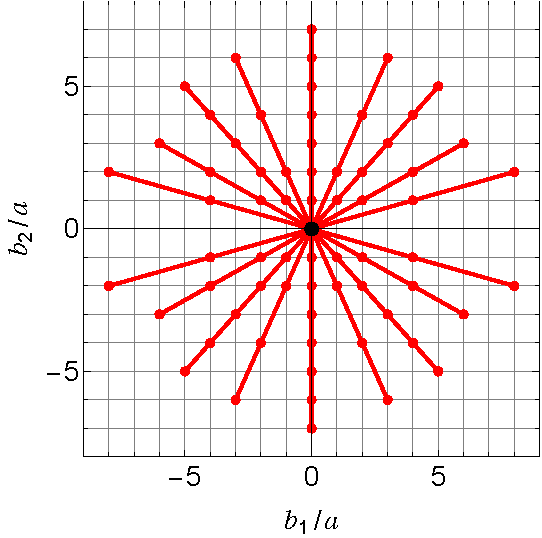
\includegraphics[width=\linewidth]{plots/kinematics_interpolation/bL_bT_plot.pdf}
        \caption{Caption for plot with path}
        \label{fig:bL_bT_path}
    \end{minipage}\hfill
    \begin{minipage}{0.45\textwidth}
        \centering
        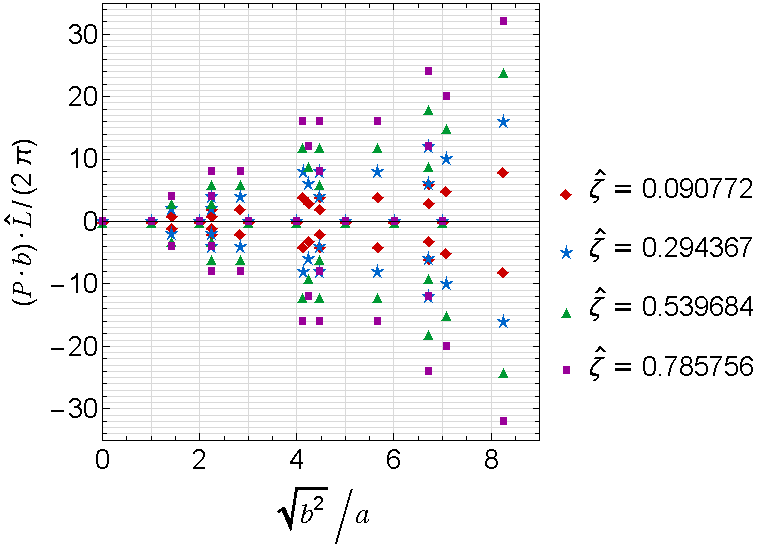
\includegraphics[width=\linewidth]{plots/kinematics_interpolation/Pb_bsq_plot.pdf}
        \caption{Caption for standard plot}
        \label{fig:bL_bT_standard}
    \end{minipage}
\end{figure}

\begin{figure}[h!]
    \centering
    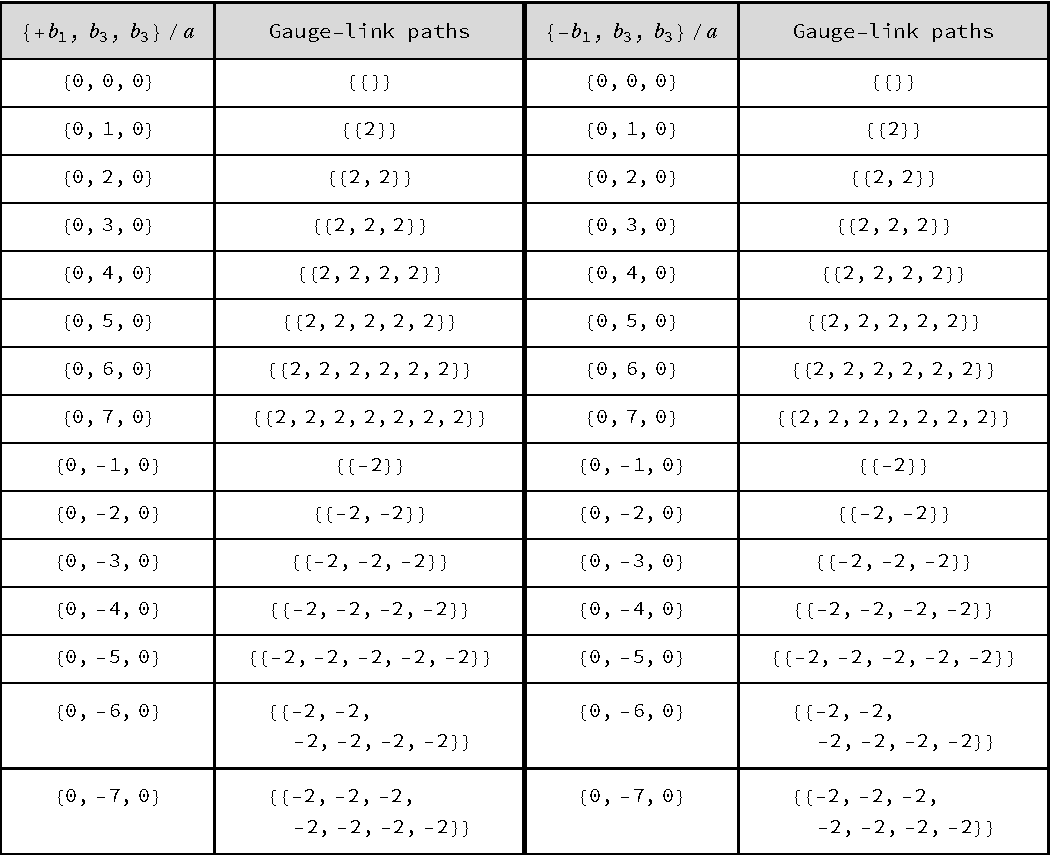
\includegraphics[width=0.5\linewidth]{plots/kinematics_interpolation/b_gauge_links_for_table1.pdf}
    \caption{Caption}
    \label{fig:placeholder}
\end{figure}
\begin{figure}[h!]
    \centering
    \begin{minipage}{0.45\textwidth}
        \centering
        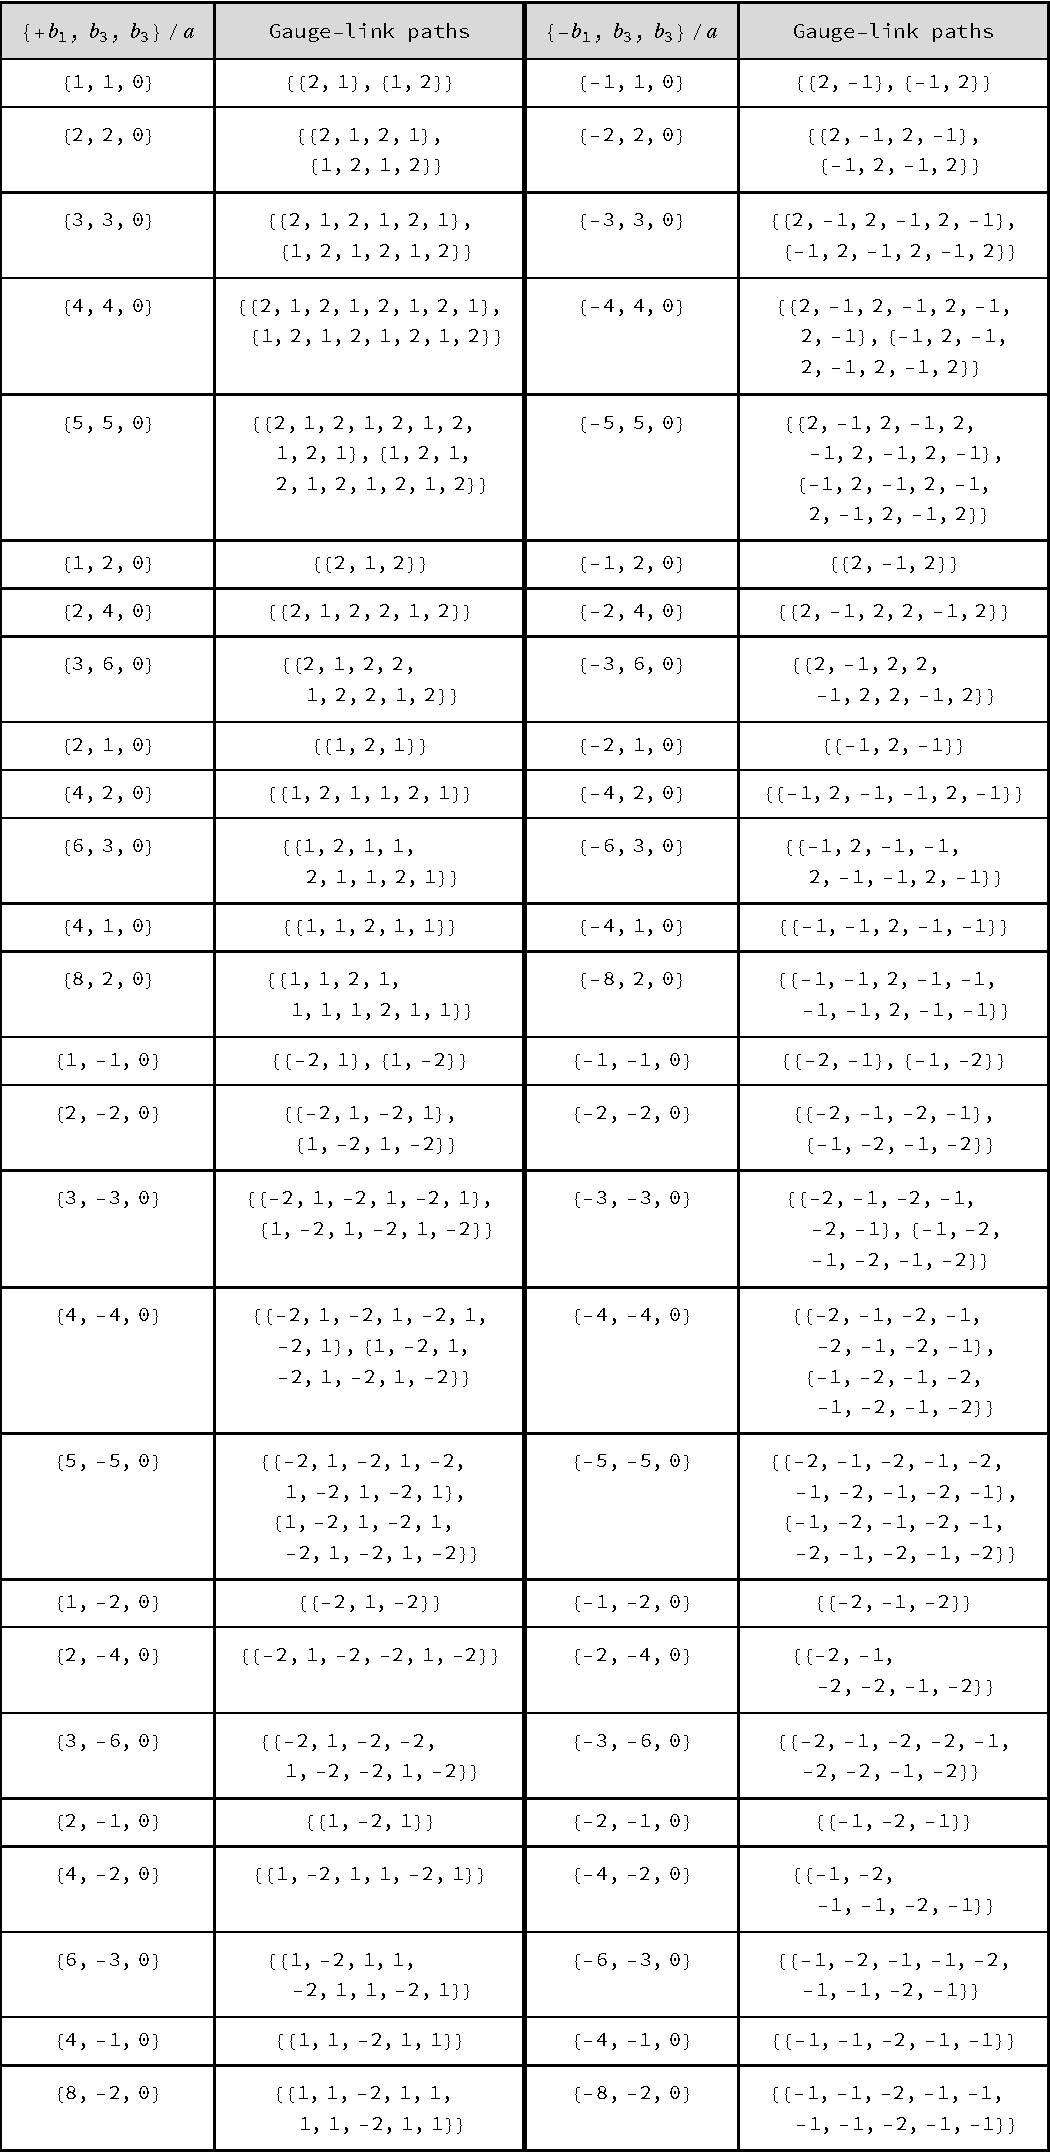
\includegraphics[width=\linewidth]{plots/kinematics_interpolation/b_gauge_links_for_table2.pdf}
        \caption{First caption}
        \label{fig:placeholder1}
    \end{minipage}\hfill
    \begin{minipage}{0.45\textwidth}
        \centering
        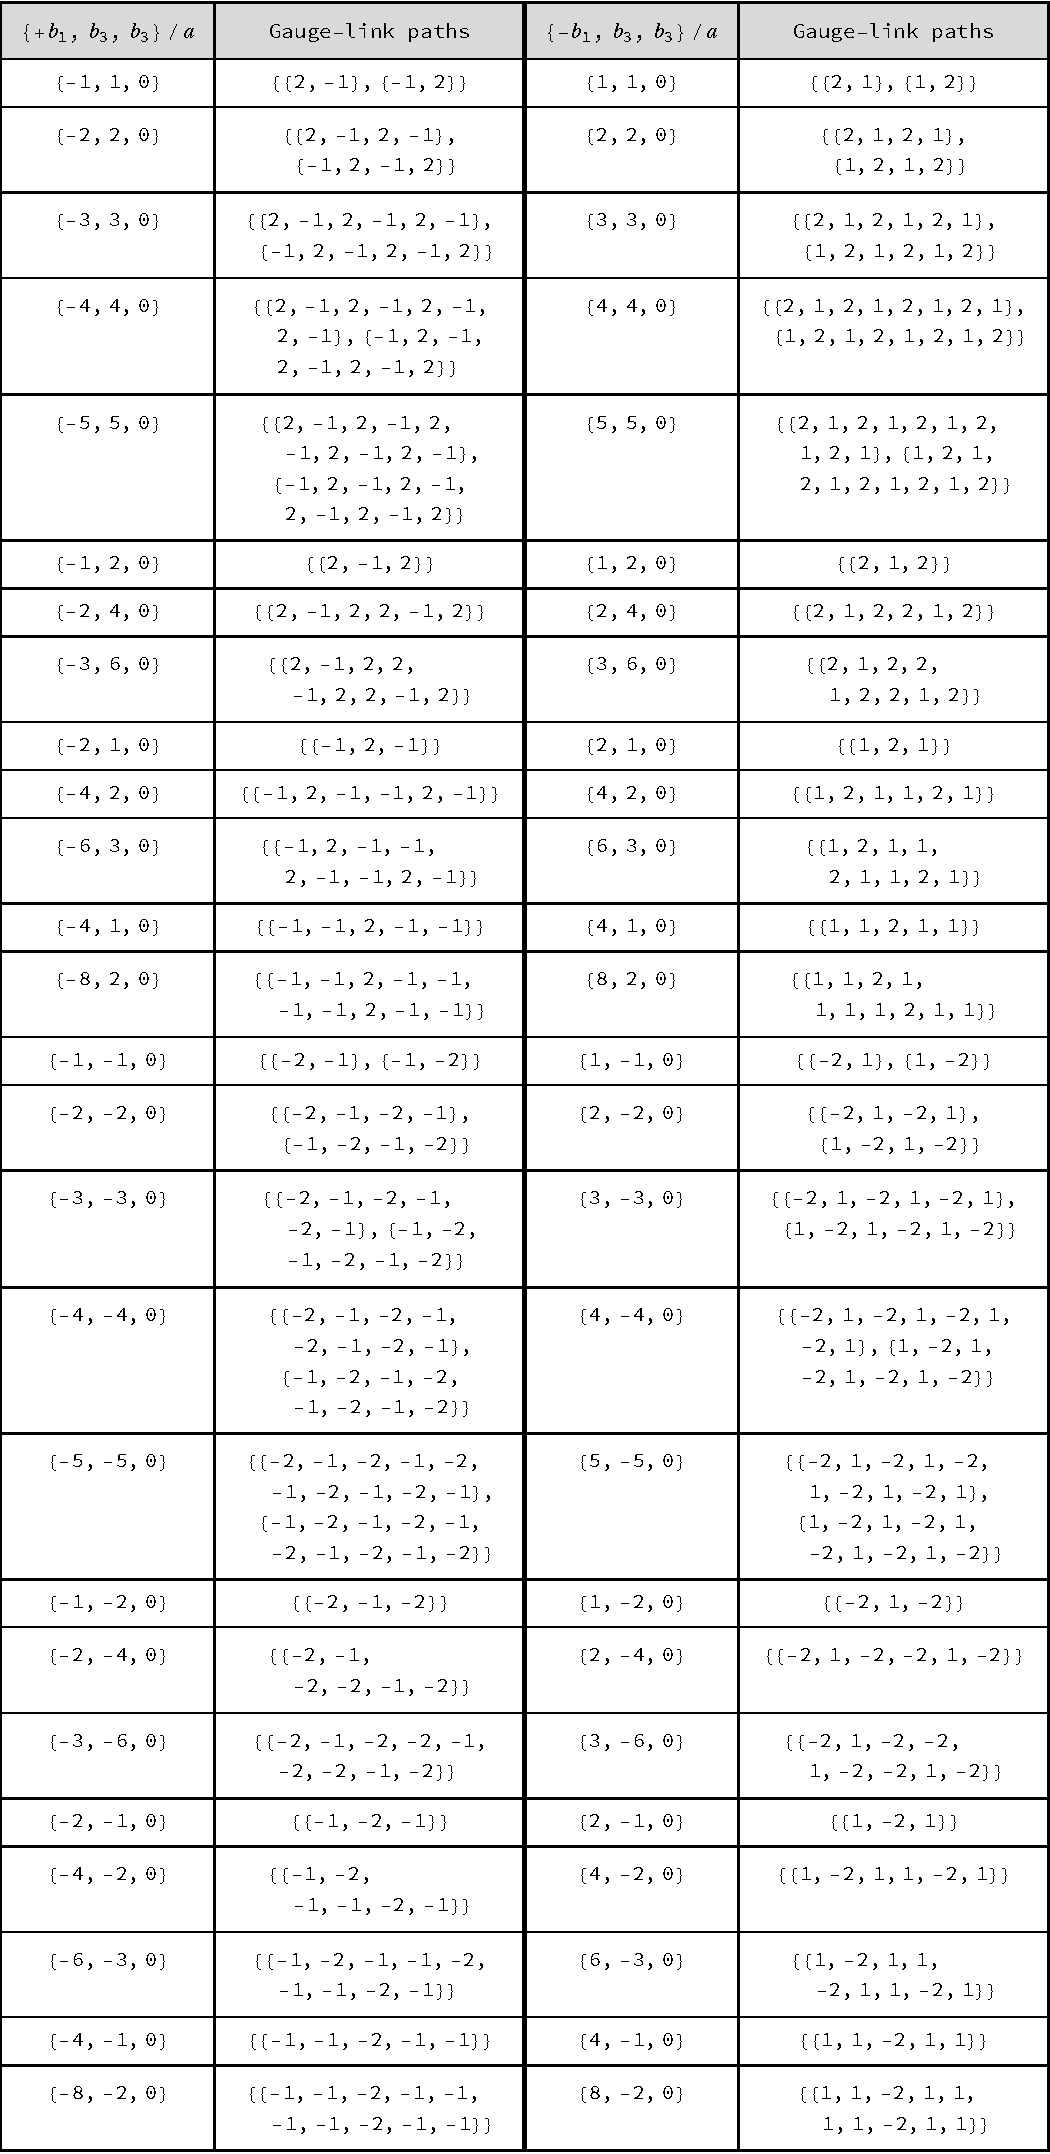
\includegraphics[width=\linewidth]{plots/kinematics_interpolation/b_gauge_links_for_table3.pdf}
        \caption{Second caption}
        \label{fig:placeholder2}
    \end{minipage}
\end{figure}

\pagebreak
Same $\vect{b}$ with different linkpaths are averaged
\begin{figure}[h!]
    \centering
    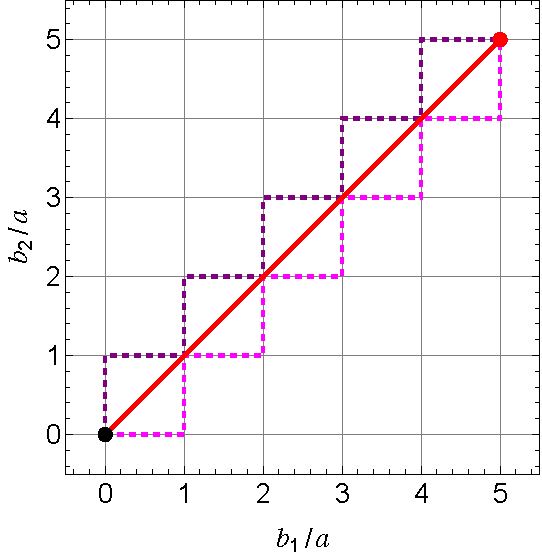
\includegraphics[width=0.3\linewidth]{plots/kinematics_interpolation/Example_b_plot_with_2path.pdf}
    \caption{Caption}
    \label{fig:placeholder}
\end{figure}
\begin{figure}[h!]
    \centering
    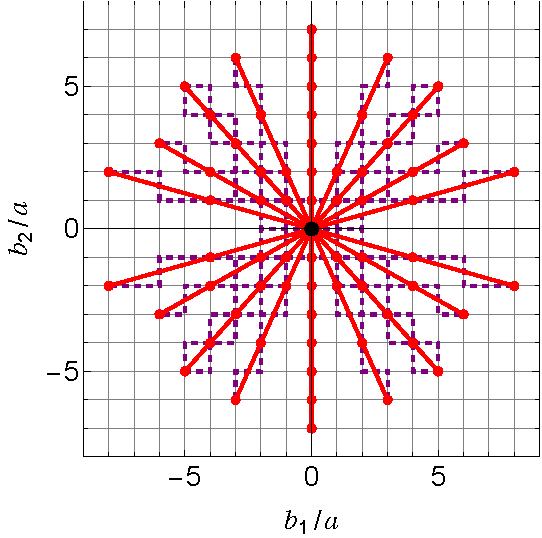
\includegraphics[width=0.5\linewidth]{plots/kinematics_interpolation/bL_bT_plot_with_path.pdf}
    \caption{Caption}
    \label{fig:placeholder}
\end{figure}

\pagebreak
\subsubsection{\texorpdfstring{$\vect{v}$}{TEXT} - Interpolation}
Same $\vect{v}$ with different sidelink are averaged
\begin{figure}[h!]
    \centering
    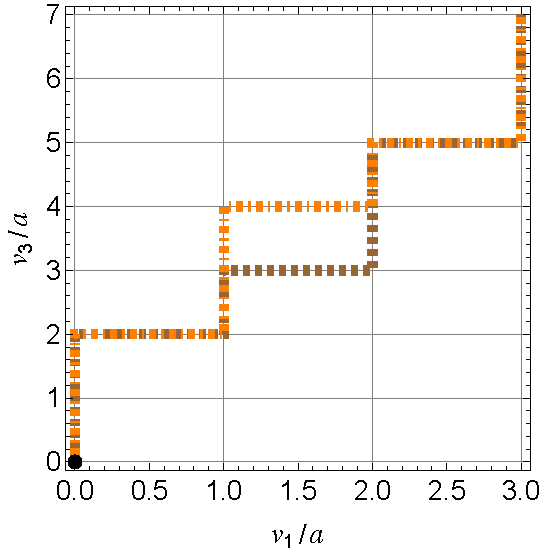
\includegraphics[width=0.5\linewidth]{plots/kinematics_interpolation/Example_v_plot_with_2path.pdf}
    \caption{Caption}
    \label{fig:placeholder}
\end{figure}
\begin{figure}[h!]
    \centering
    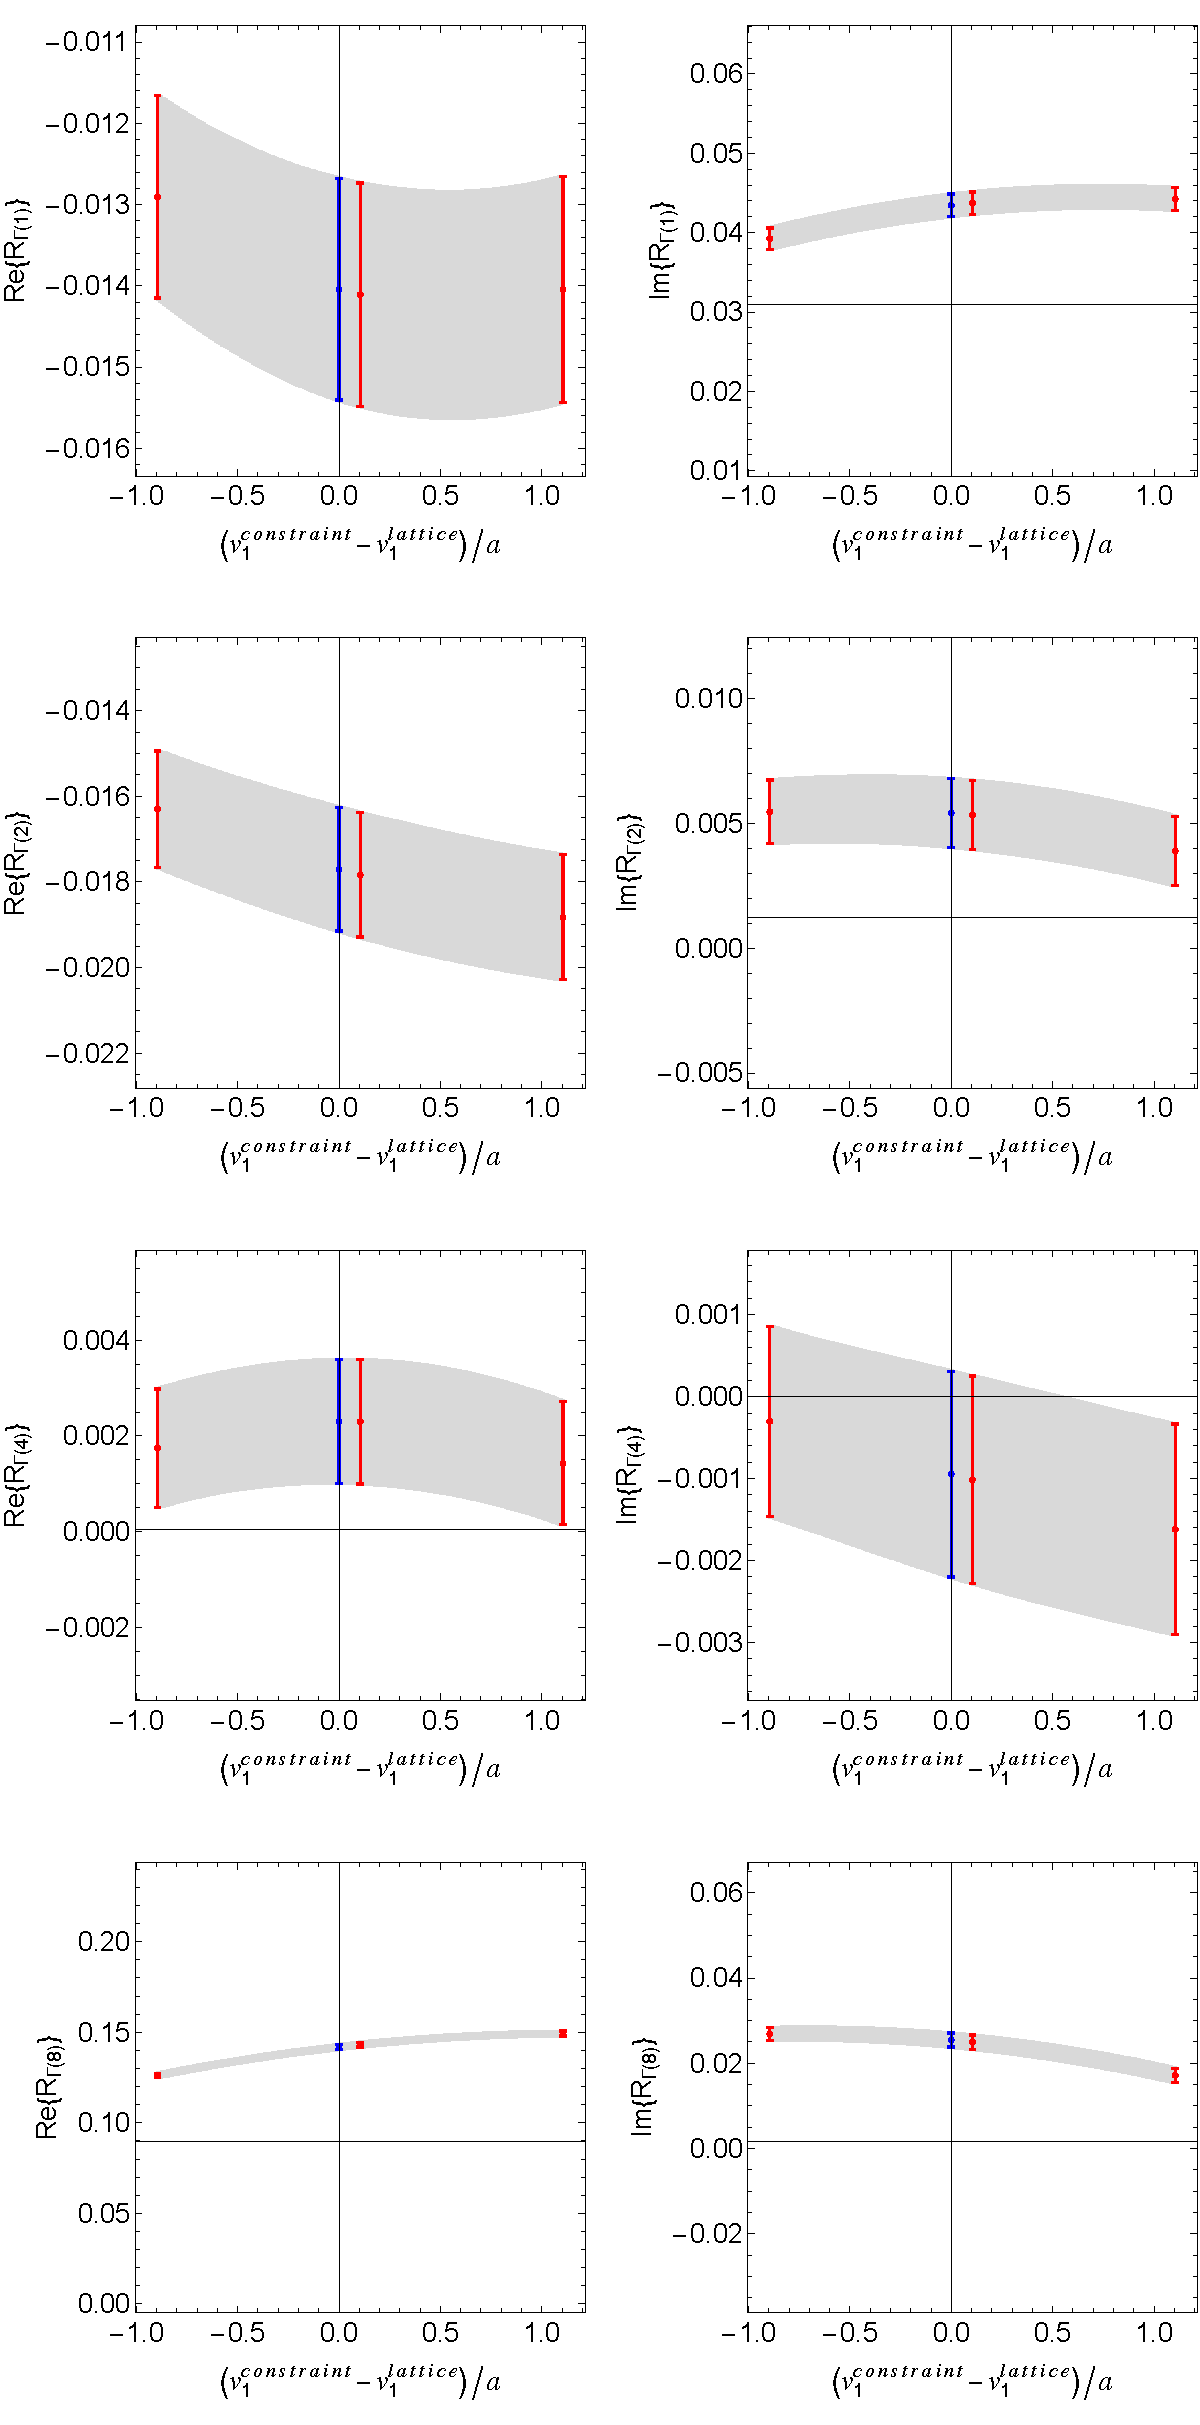
\includegraphics[width=0.6\linewidth]{plots/kinematics_interpolation/Interpolation_Ex_b120_eta7_P-1.pdf}
    \caption{Interpolation Example for $\vect{b}={1,2,0}$, $\eta=7$, $P_L\cdot a\hat{L}/(2\pi)=-1$}
    \label{fig:placeholder}
\end{figure}

\pagebreak
\subsection{Lattice calculations of Amplitudes}
\subsubsection{\texorpdfstring{$\hat{\zeta}=0.090772$}{TEXT}}
\begin{figure}
    \centering
    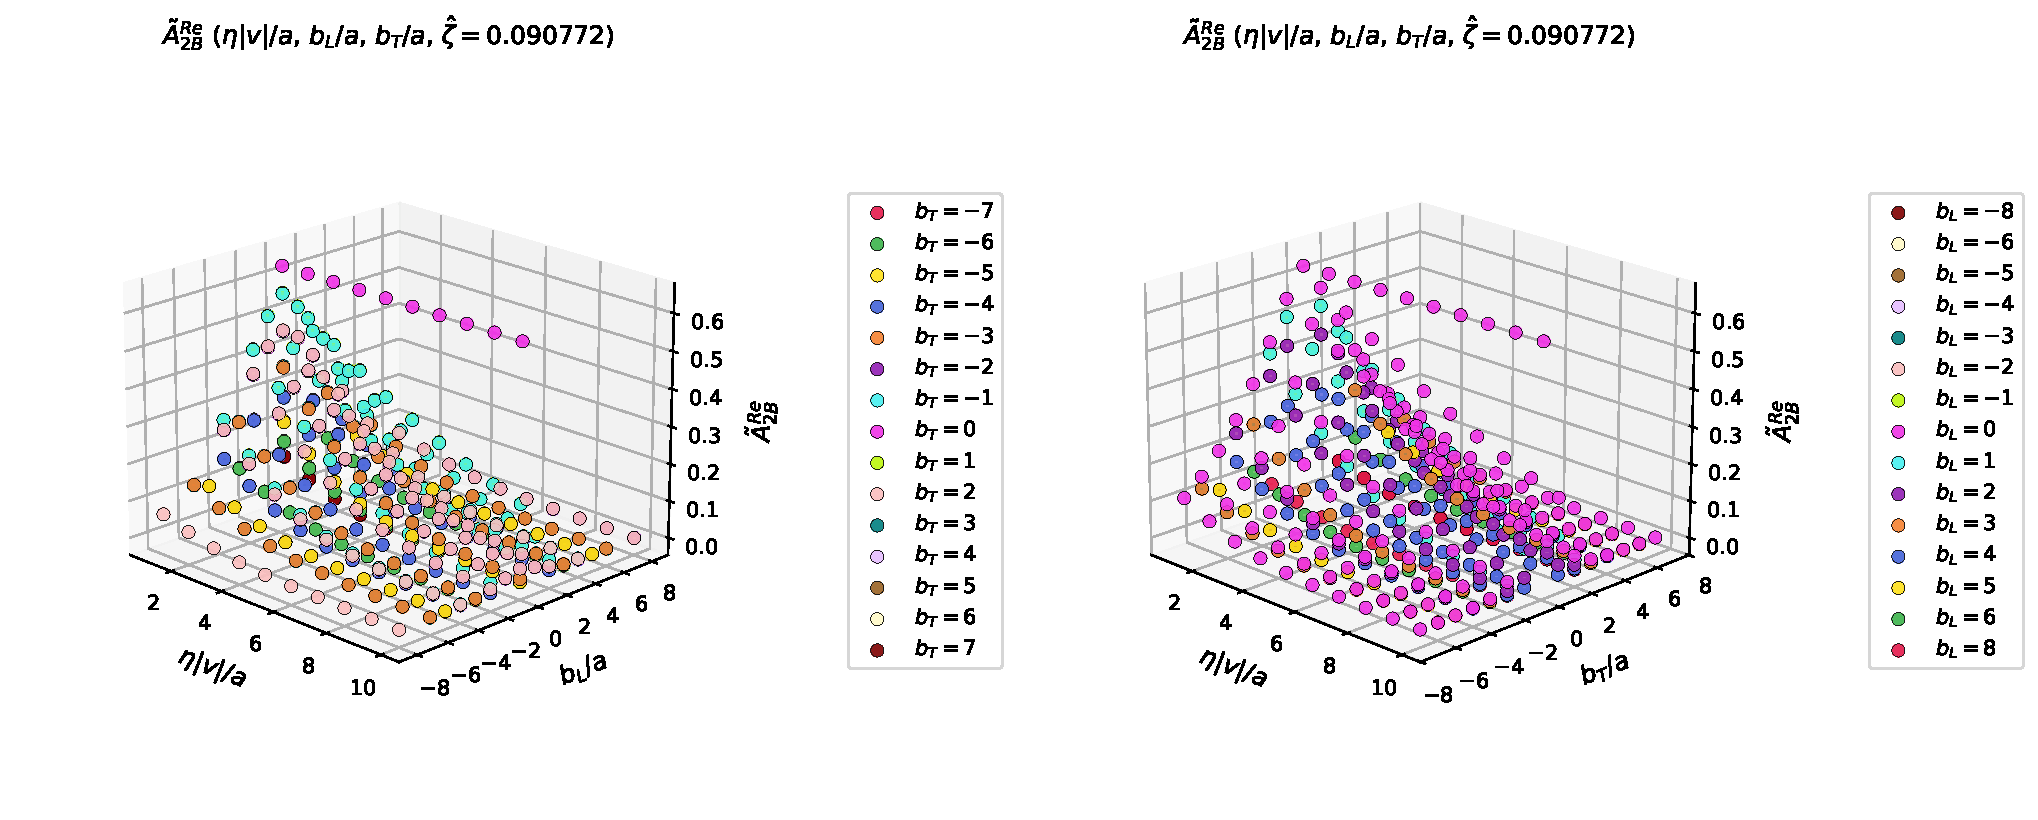
\includegraphics[width=0.7\linewidth]{plots/Amps_bL_bT/ReA2B_PL-1_3D.pdf}
    \caption{Caption}
    \label{fig:placeholder}
\end{figure}
\begin{figure}
    \centering
    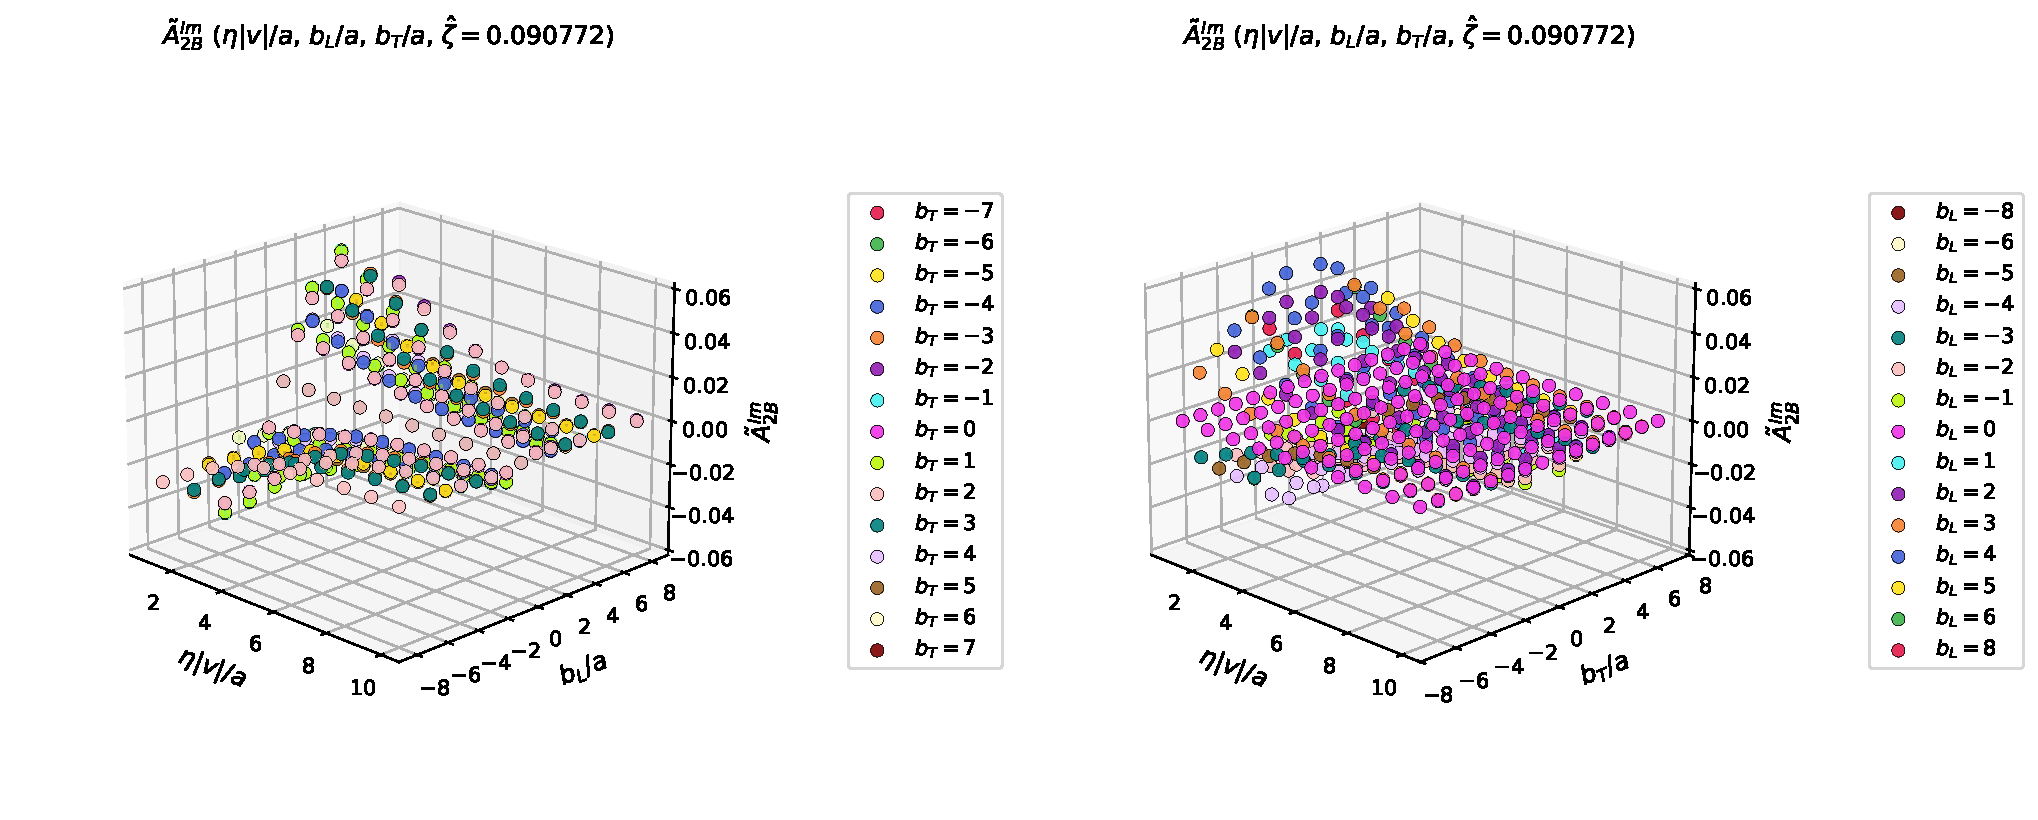
\includegraphics[width=0.7\linewidth]{plots/Amps_bL_bT/ImA2B_PL-1_3D.pdf}
    \caption{Caption}
    \label{fig:placeholder}
\end{figure}
\begin{figure}
    \centering
    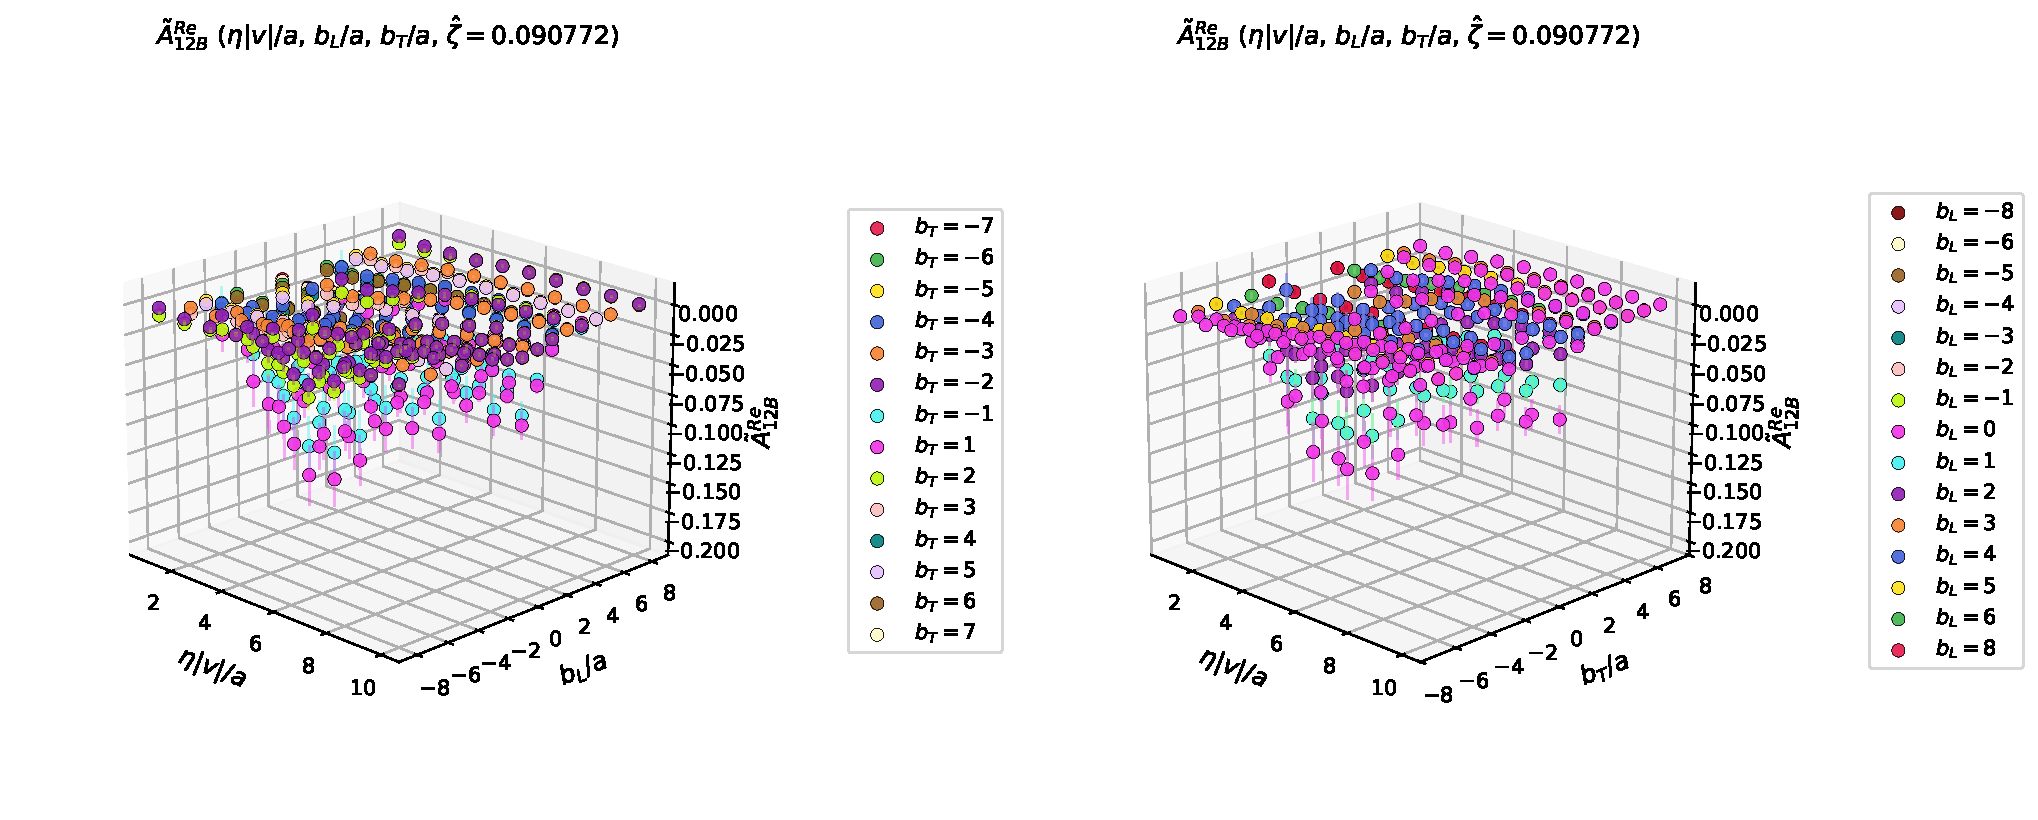
\includegraphics[width=0.7\linewidth]{plots/Amps_bL_bT/ReA12B_PL-1_3D.pdf}
    \caption{Caption}
    \label{fig:placeholder}
\end{figure}
\begin{figure}
    \centering
    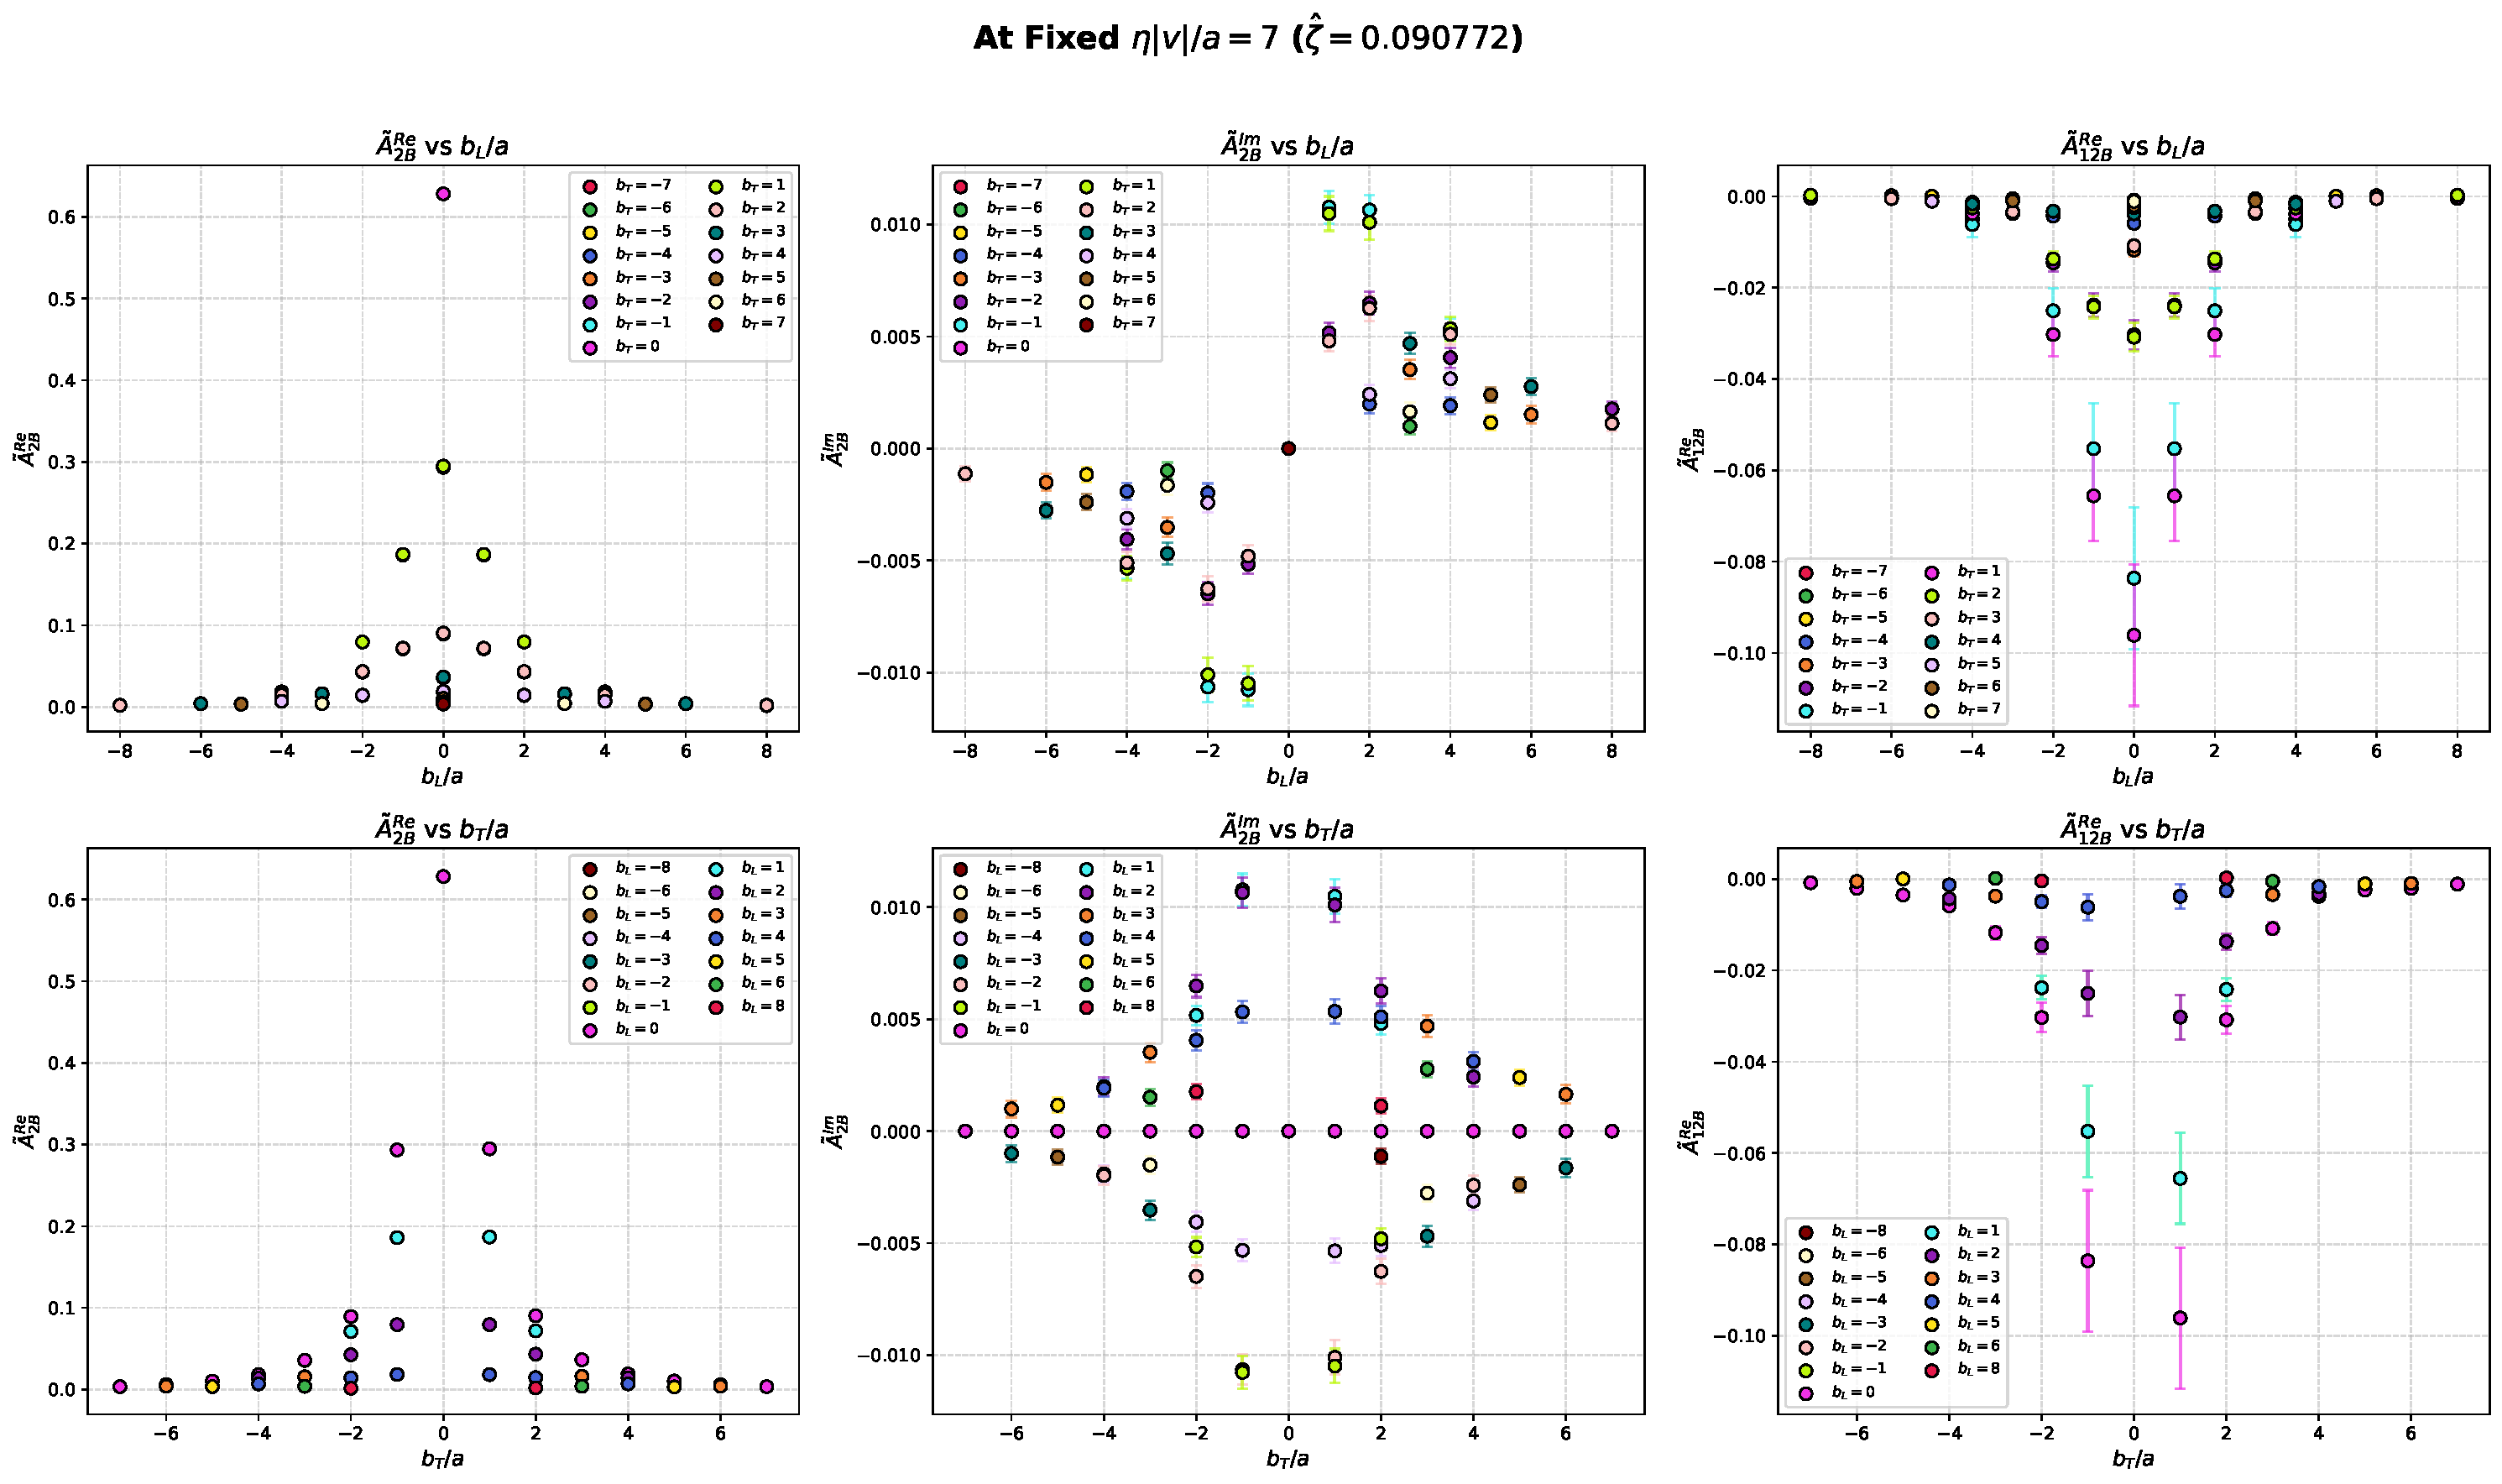
\includegraphics[width=0.7\linewidth]{plots/Amps_bL_bT/Combined_2D_eta7_PL-1.pdf}
    \caption{Caption}
    \label{fig:placeholder}
\end{figure}

\pagebreak
\subsubsection{\texorpdfstring{$\hat{\zeta}=0.294367$}{TEXT}}
\begin{figure}
    \centering
    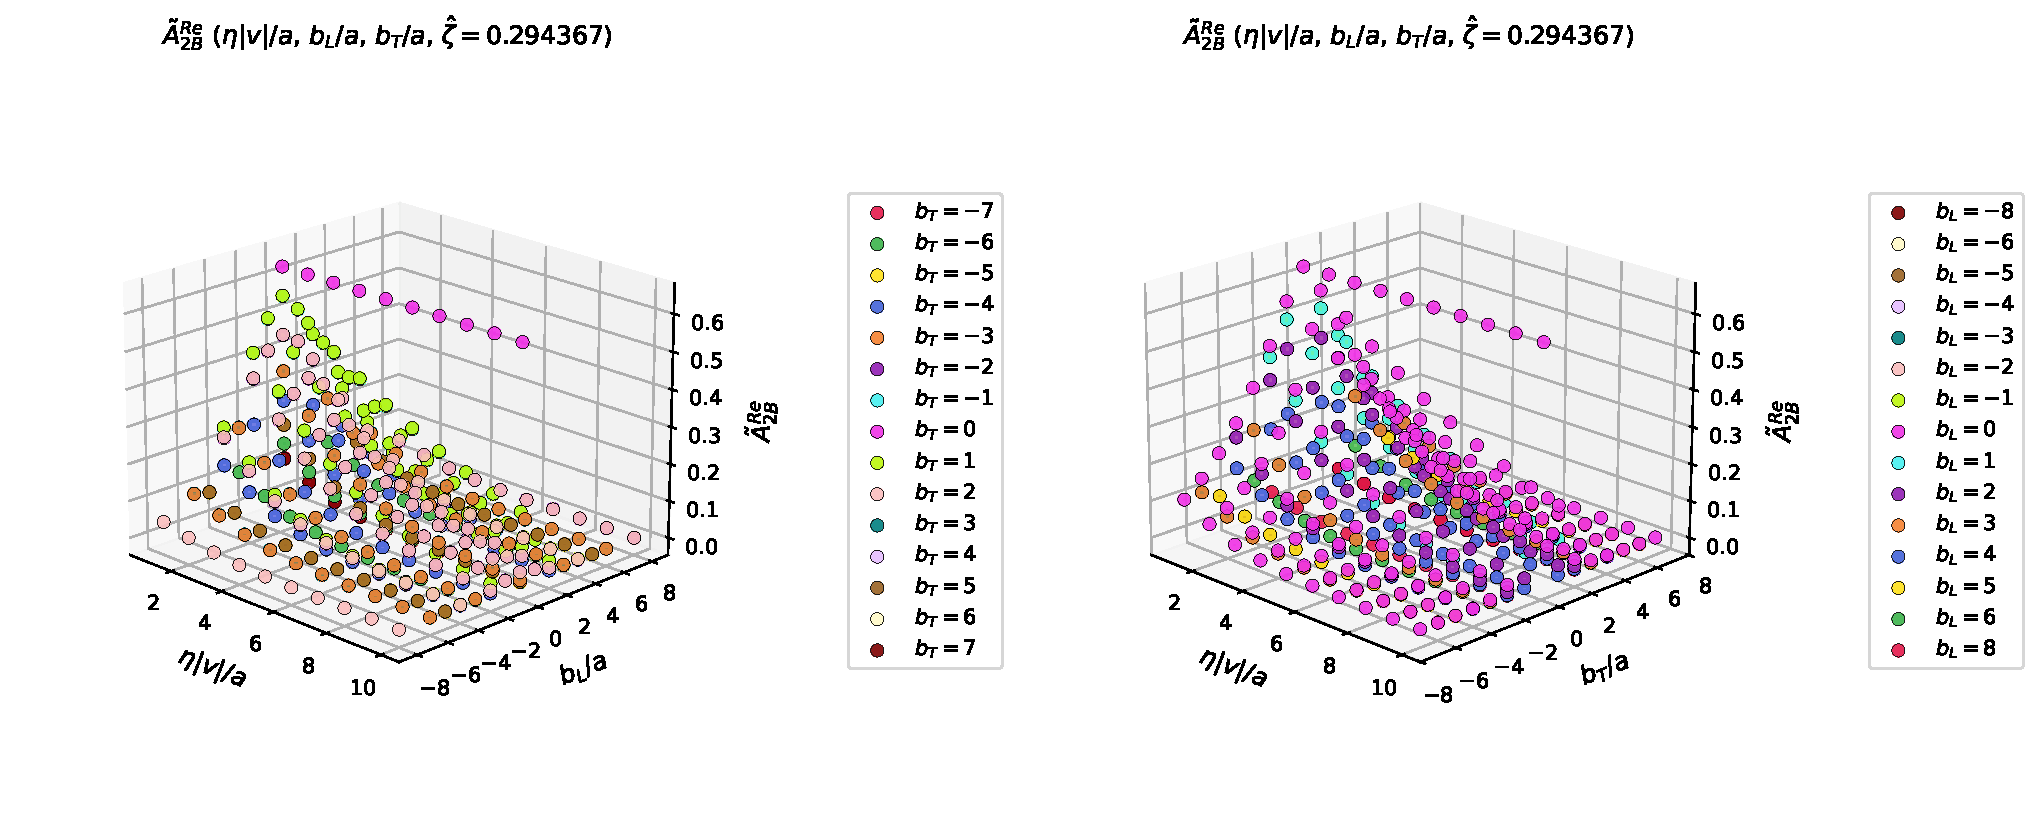
\includegraphics[width=0.7\linewidth]{plots/Amps_bL_bT/ReA2B_PL-2_3D.pdf}
    \caption{Caption}
    \label{fig:placeholder}
\end{figure}
\begin{figure}
    \centering
    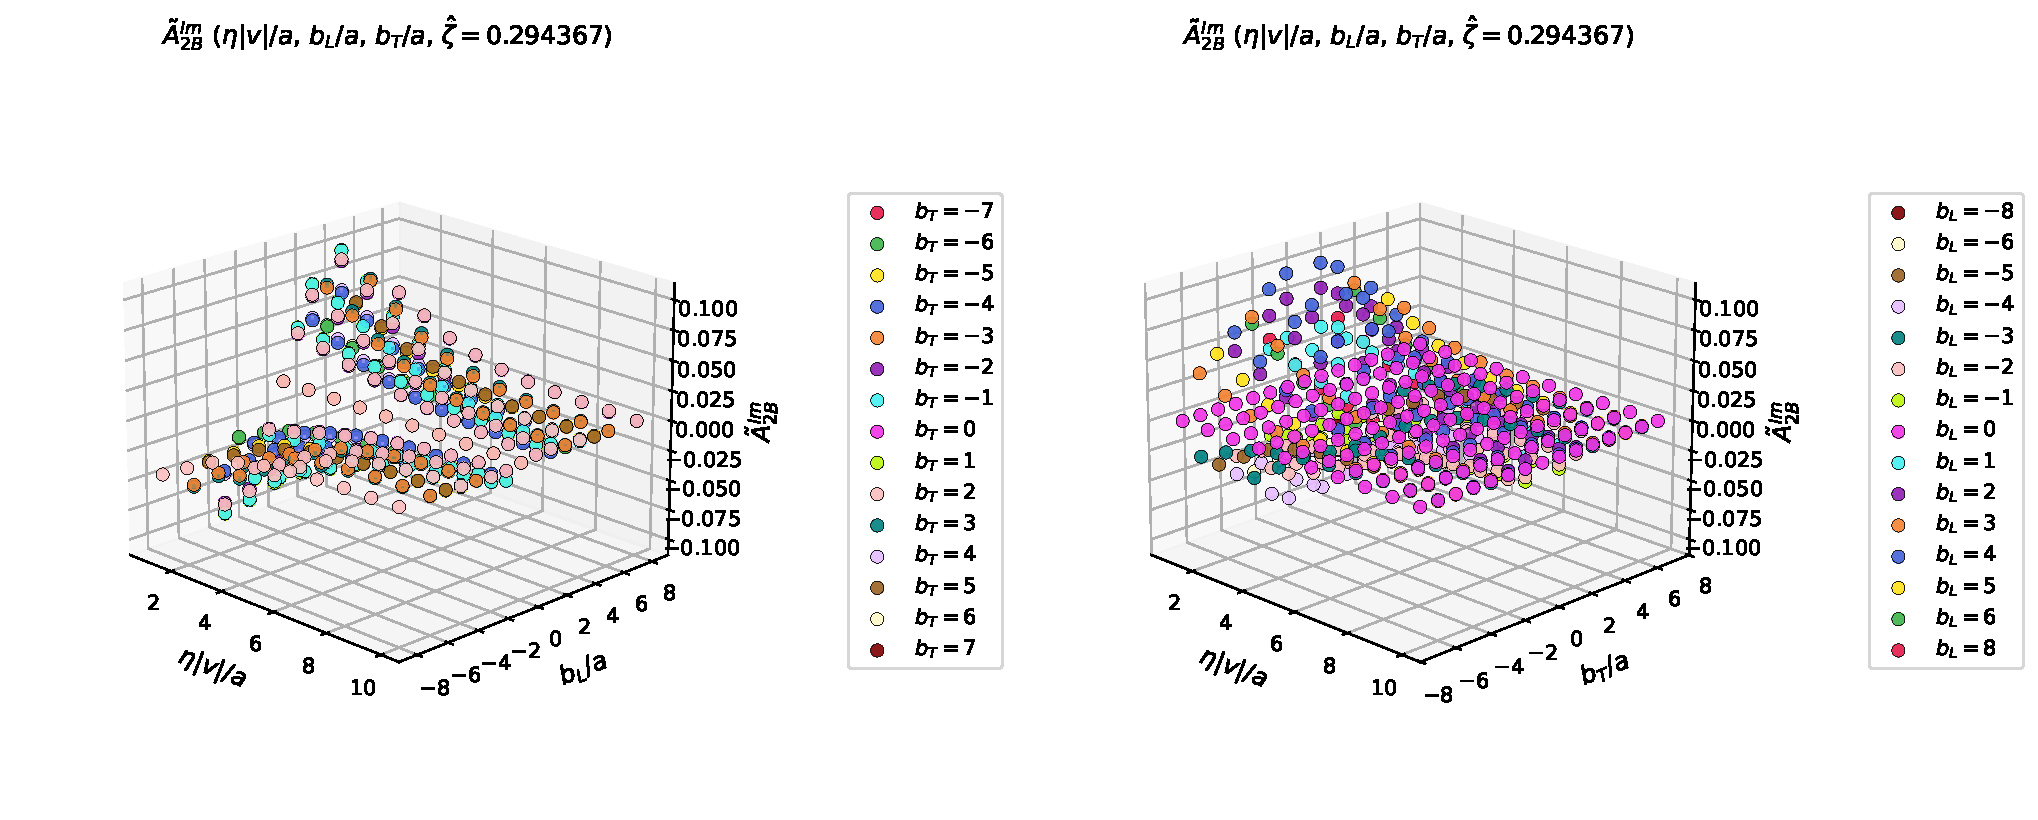
\includegraphics[width=0.7\linewidth]{plots/Amps_bL_bT/ImA2B_PL-2_3D.pdf}
    \caption{Caption}
    \label{fig:placeholder}
\end{figure}
\begin{figure}
    \centering
    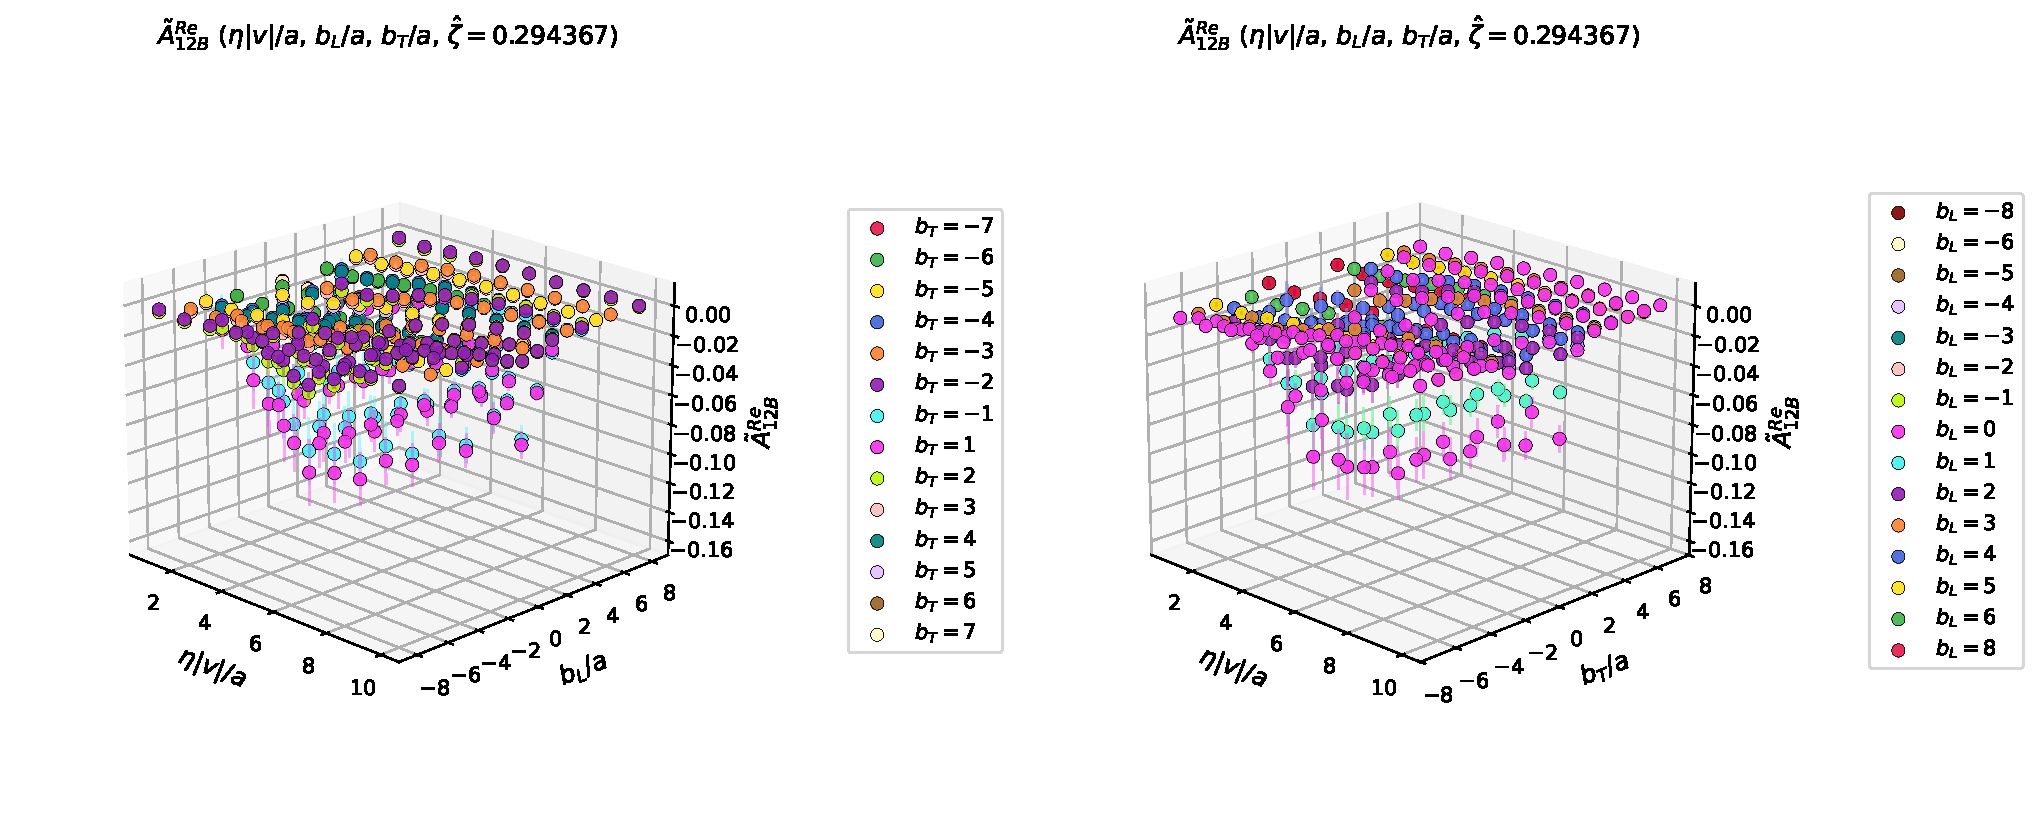
\includegraphics[width=0.7\linewidth]{plots/Amps_bL_bT/ReA12B_PL-2_3D.pdf}
    \caption{Caption}
    \label{fig:placeholder}
\end{figure}
\begin{figure}
    \centering
    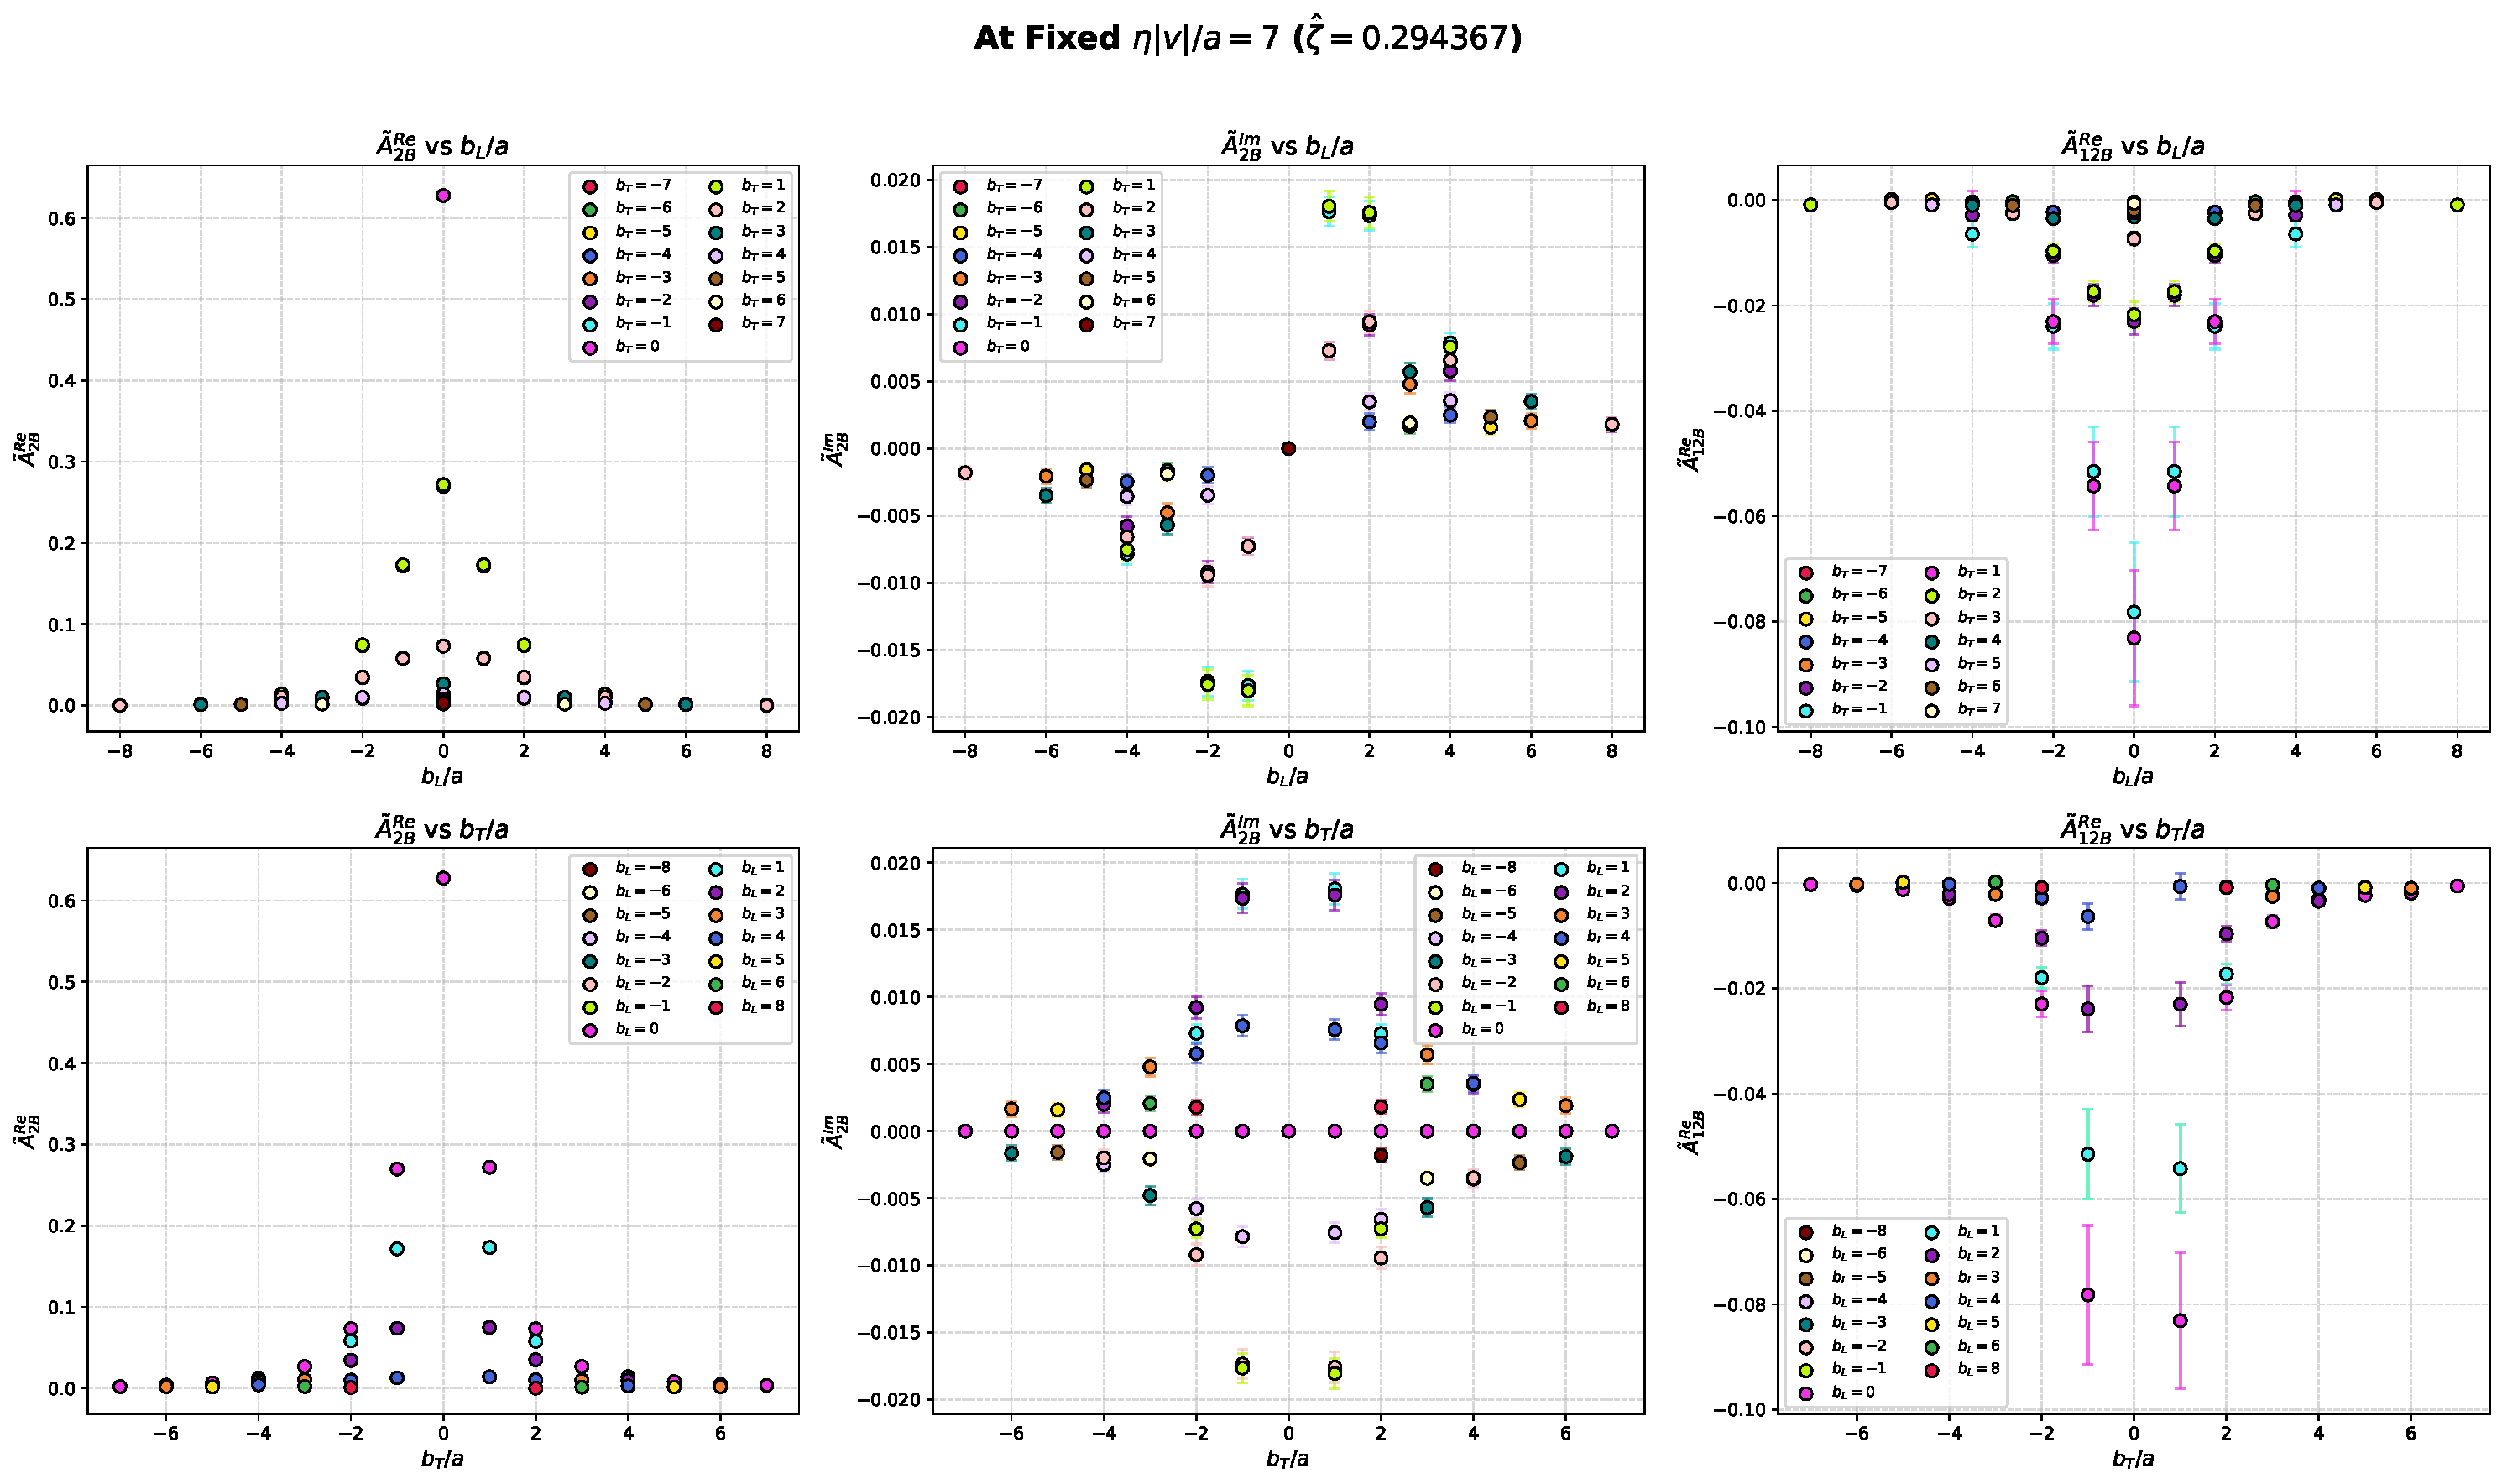
\includegraphics[width=0.7\linewidth]{plots/Amps_bL_bT/Combined_2D_eta7_PL-2.pdf}
    \caption{Caption}
    \label{fig:placeholder}
\end{figure}

\pagebreak
\subsubsection{\texorpdfstring{$\hat{\zeta}=0.539684$}{TEXT}}
\begin{figure}
    \centering
    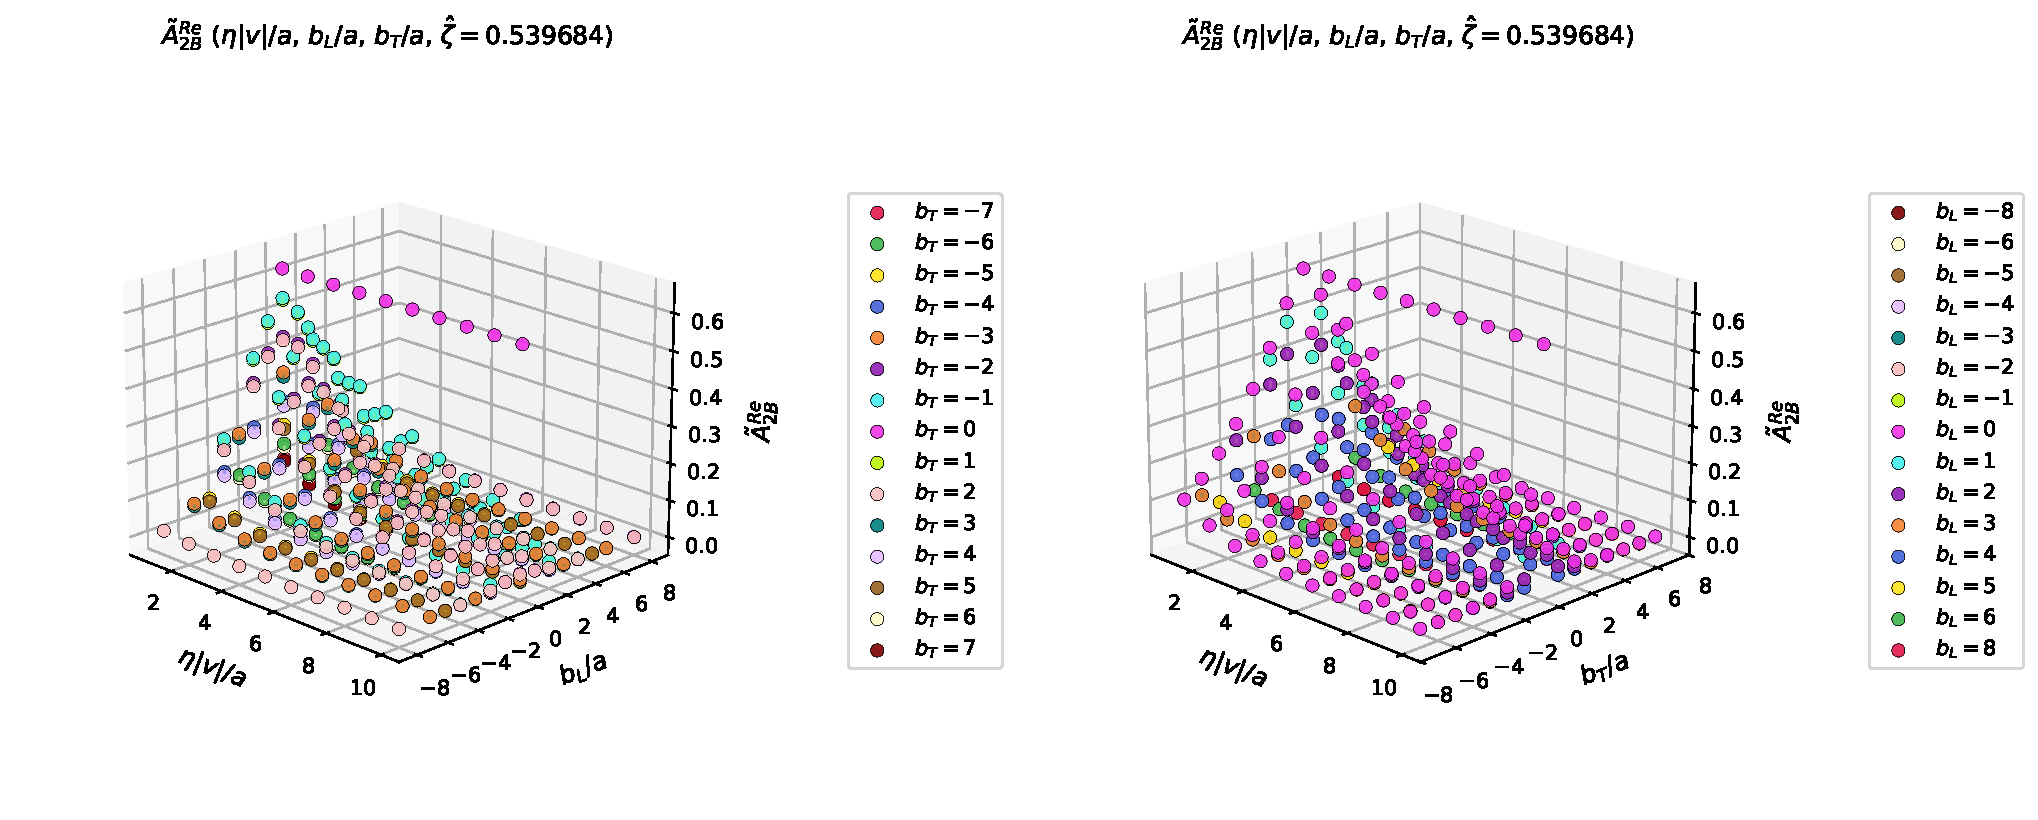
\includegraphics[width=0.7\linewidth]{plots/Amps_bL_bT/ReA2B_PL-3_3D.pdf}
    \caption{Caption}
    \label{fig:placeholder}
\end{figure}
\begin{figure}
    \centering
    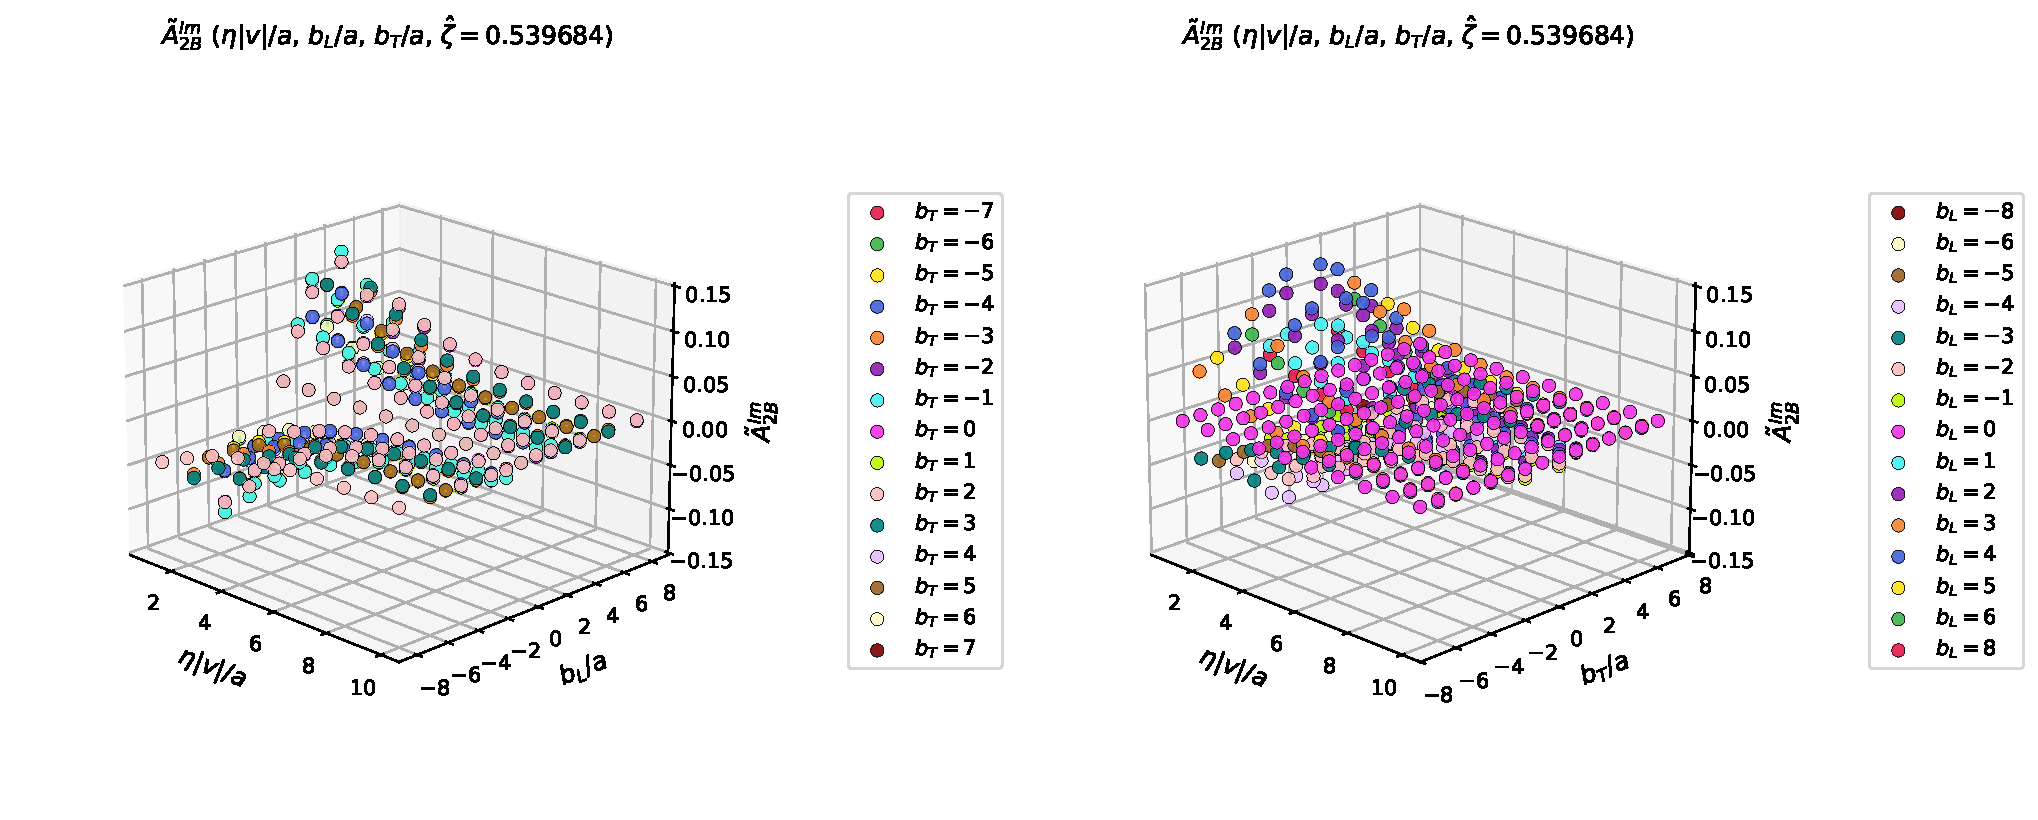
\includegraphics[width=0.7\linewidth]{plots/Amps_bL_bT/ImA2B_PL-3_3D.pdf}
    \caption{Caption}
    \label{fig:placeholder}
\end{figure}
\begin{figure}
    \centering
    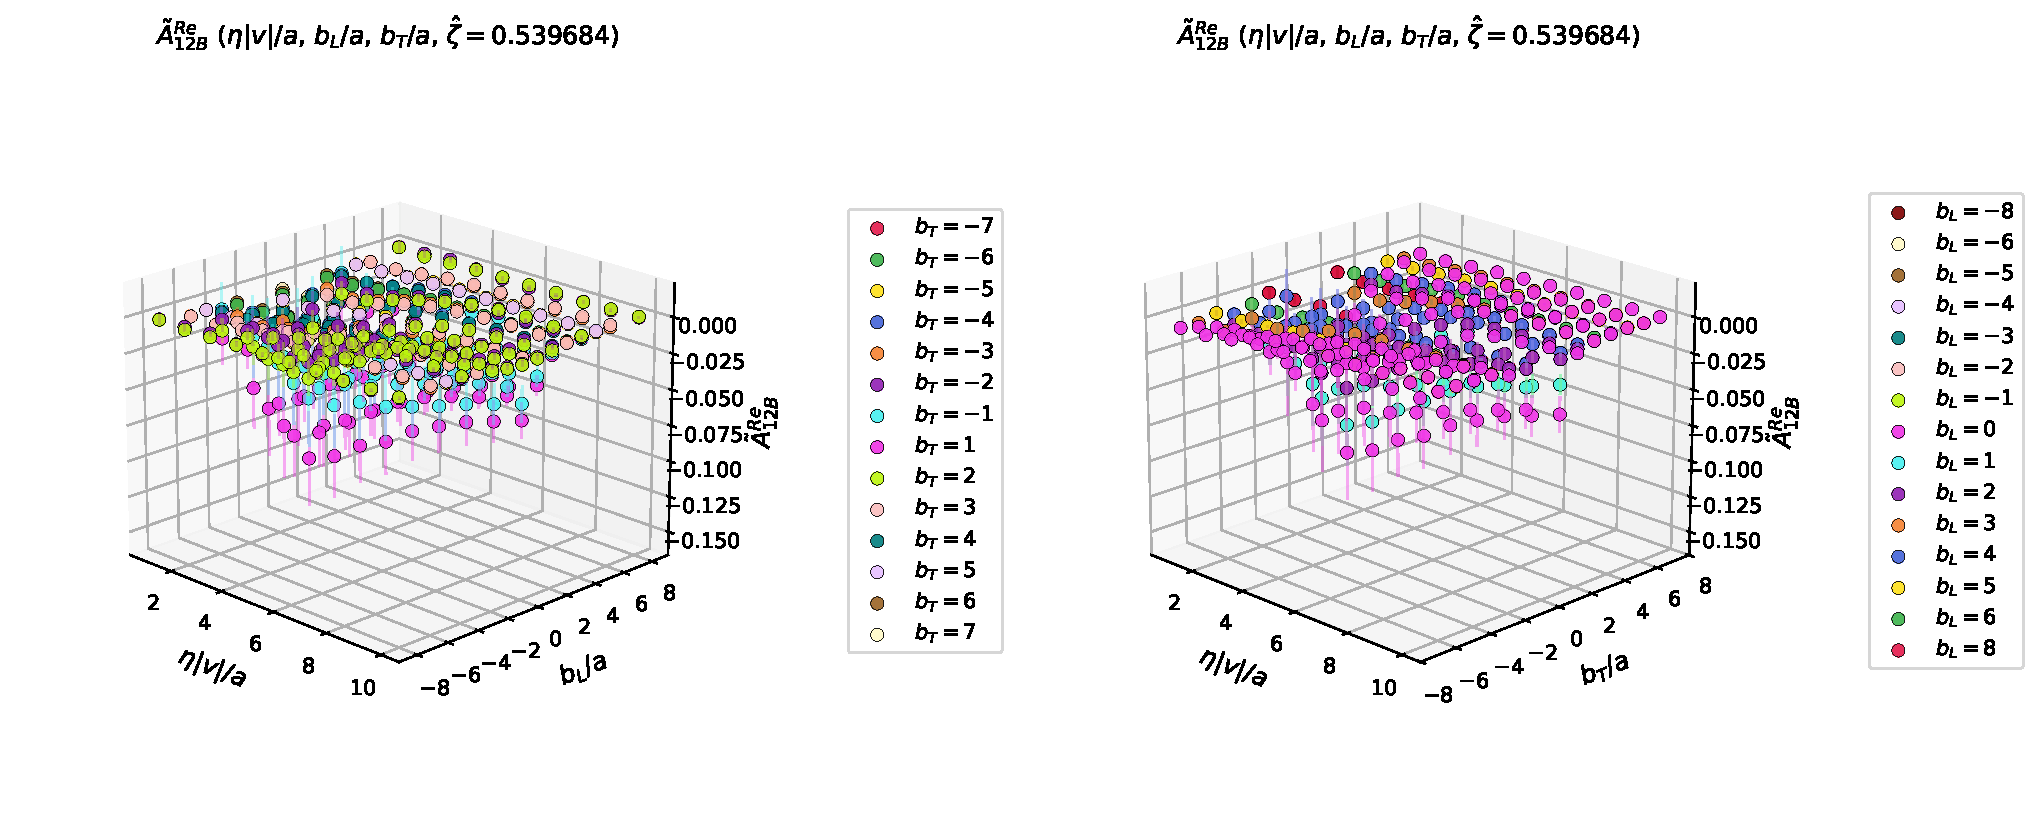
\includegraphics[width=0.7\linewidth]{plots/Amps_bL_bT/ReA12B_PL-3_3D.pdf}
    \caption{Caption}
    \label{fig:placeholder}
\end{figure}
\begin{figure}
    \centering
    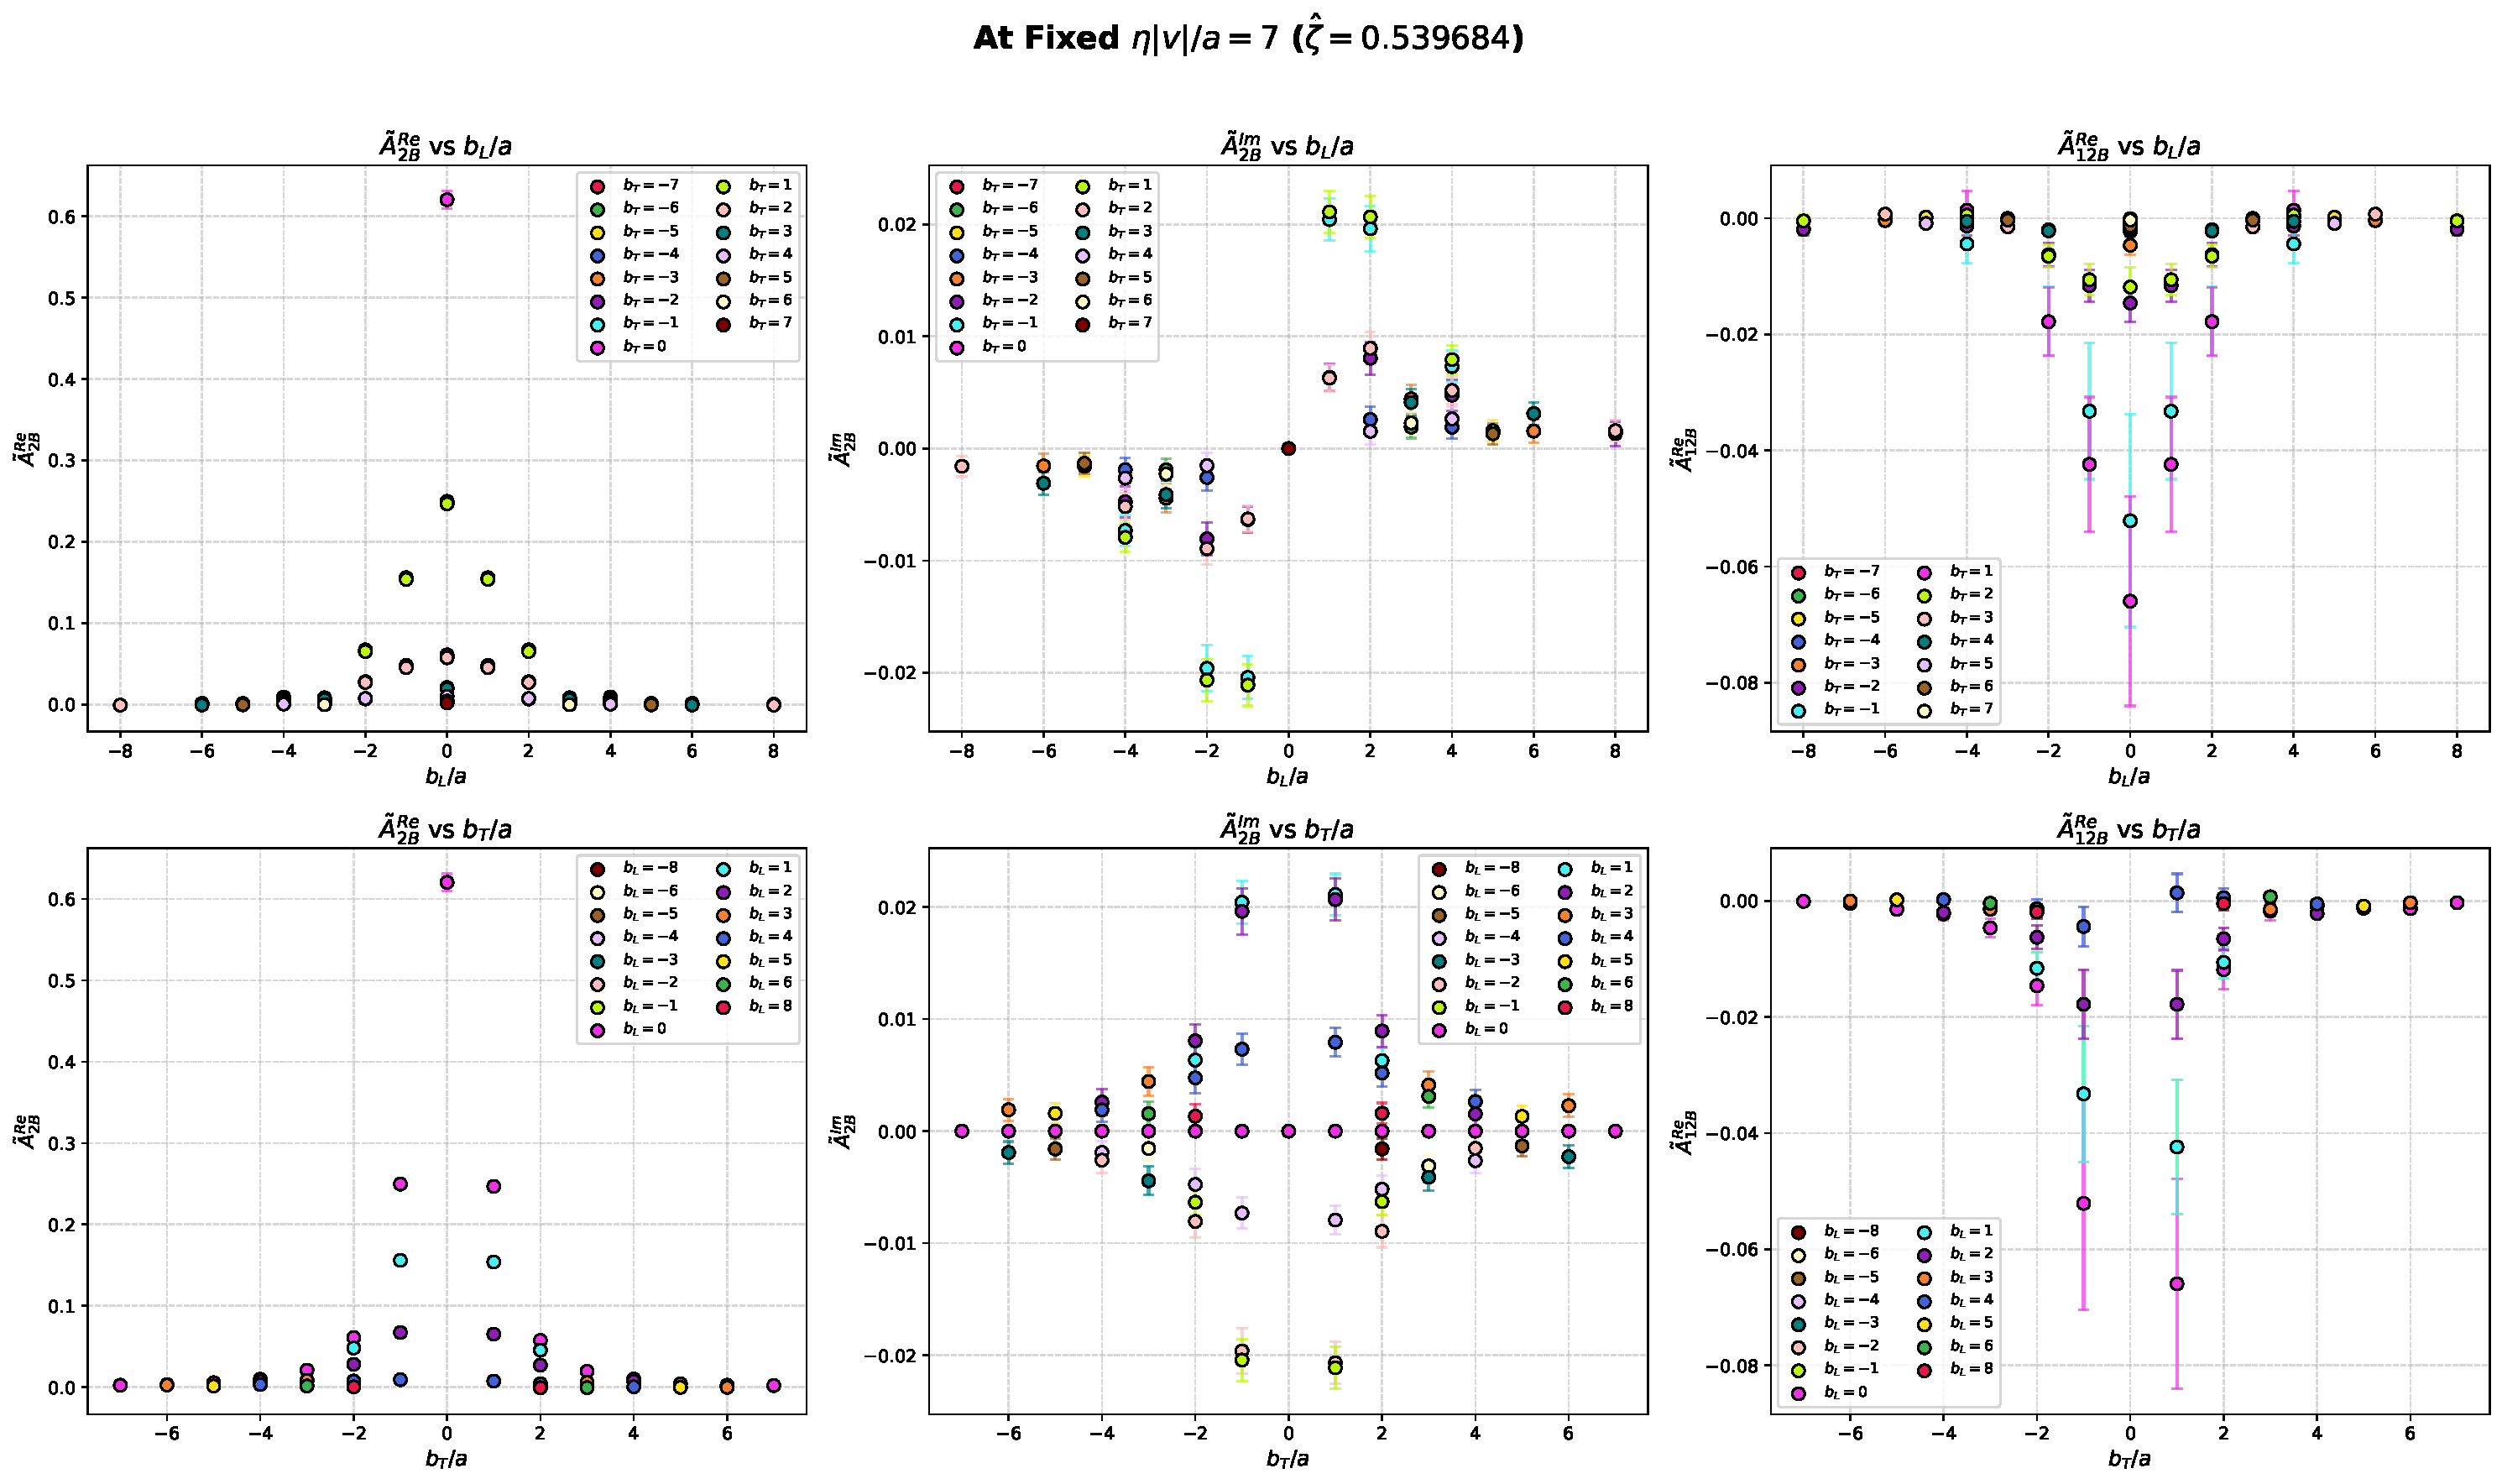
\includegraphics[width=0.7\linewidth]{plots/Amps_bL_bT/Combined_2D_eta7_PL-3.pdf}
    \caption{Caption}
    \label{fig:placeholder}
\end{figure}

\pagebreak
\subsubsection{\texorpdfstring{$\hat{\zeta}=0.785756$}{TEXT}}
\begin{figure}
    \centering
    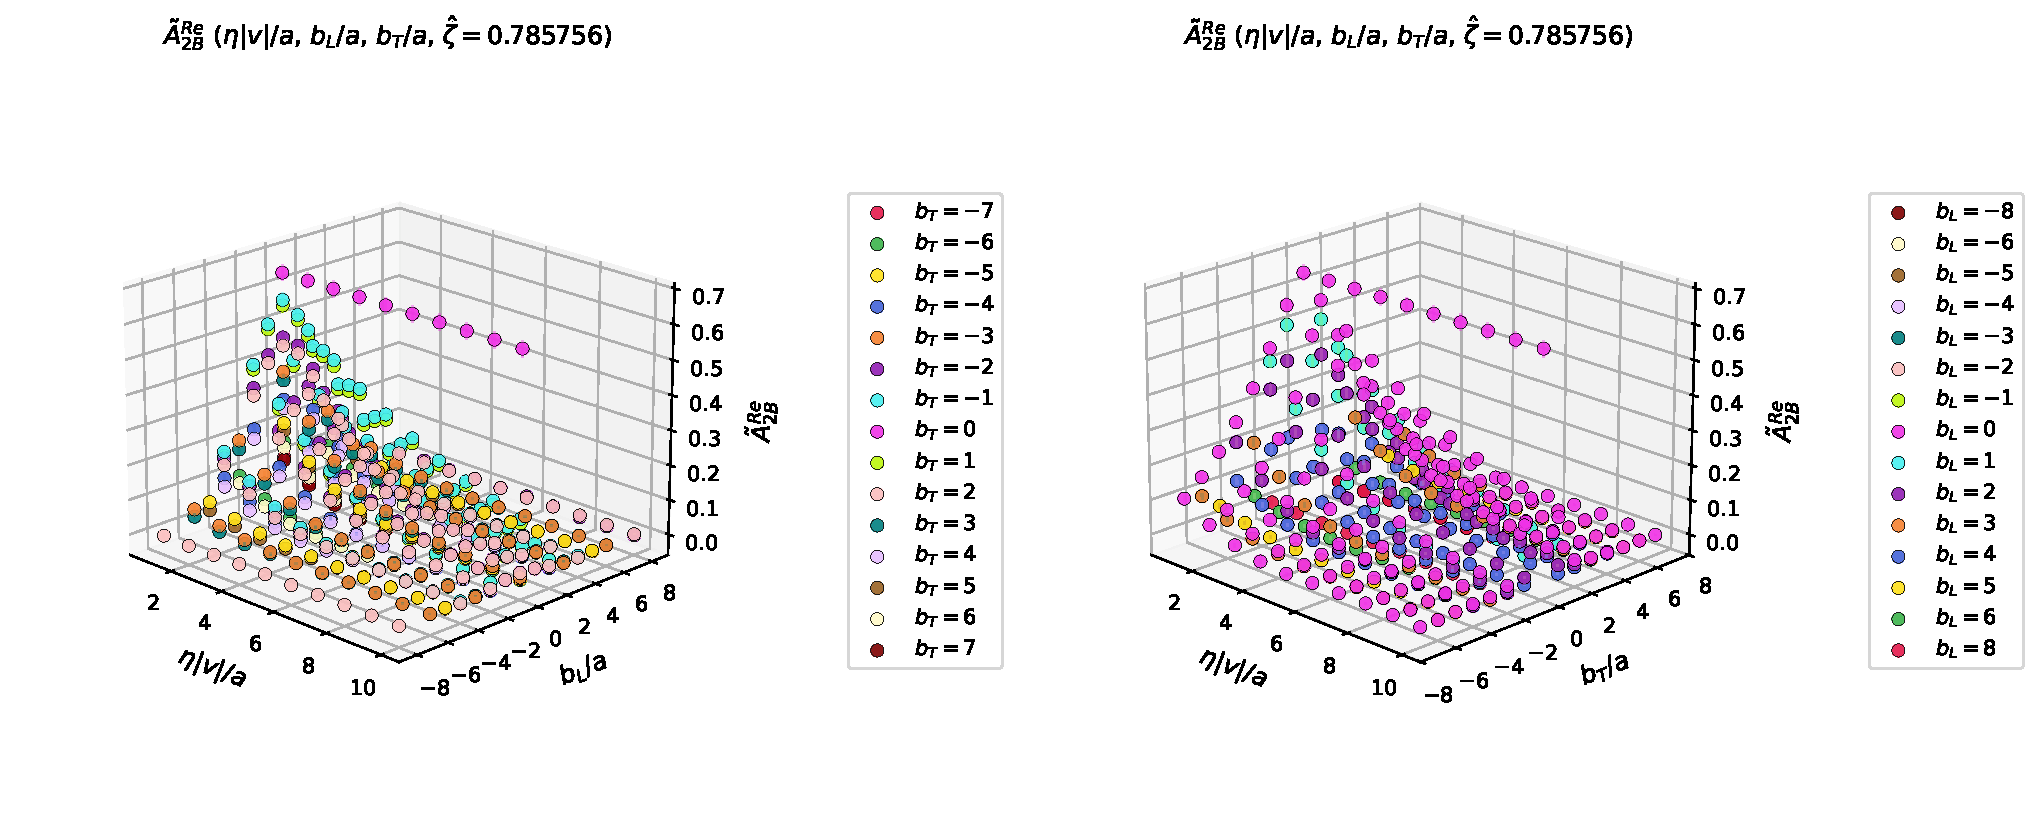
\includegraphics[width=0.7\linewidth]{plots/Amps_bL_bT/ReA2B_PL-4_3D.pdf}
    \caption{Caption}
    \label{fig:placeholder}
\end{figure}
\begin{figure}
    \centering
    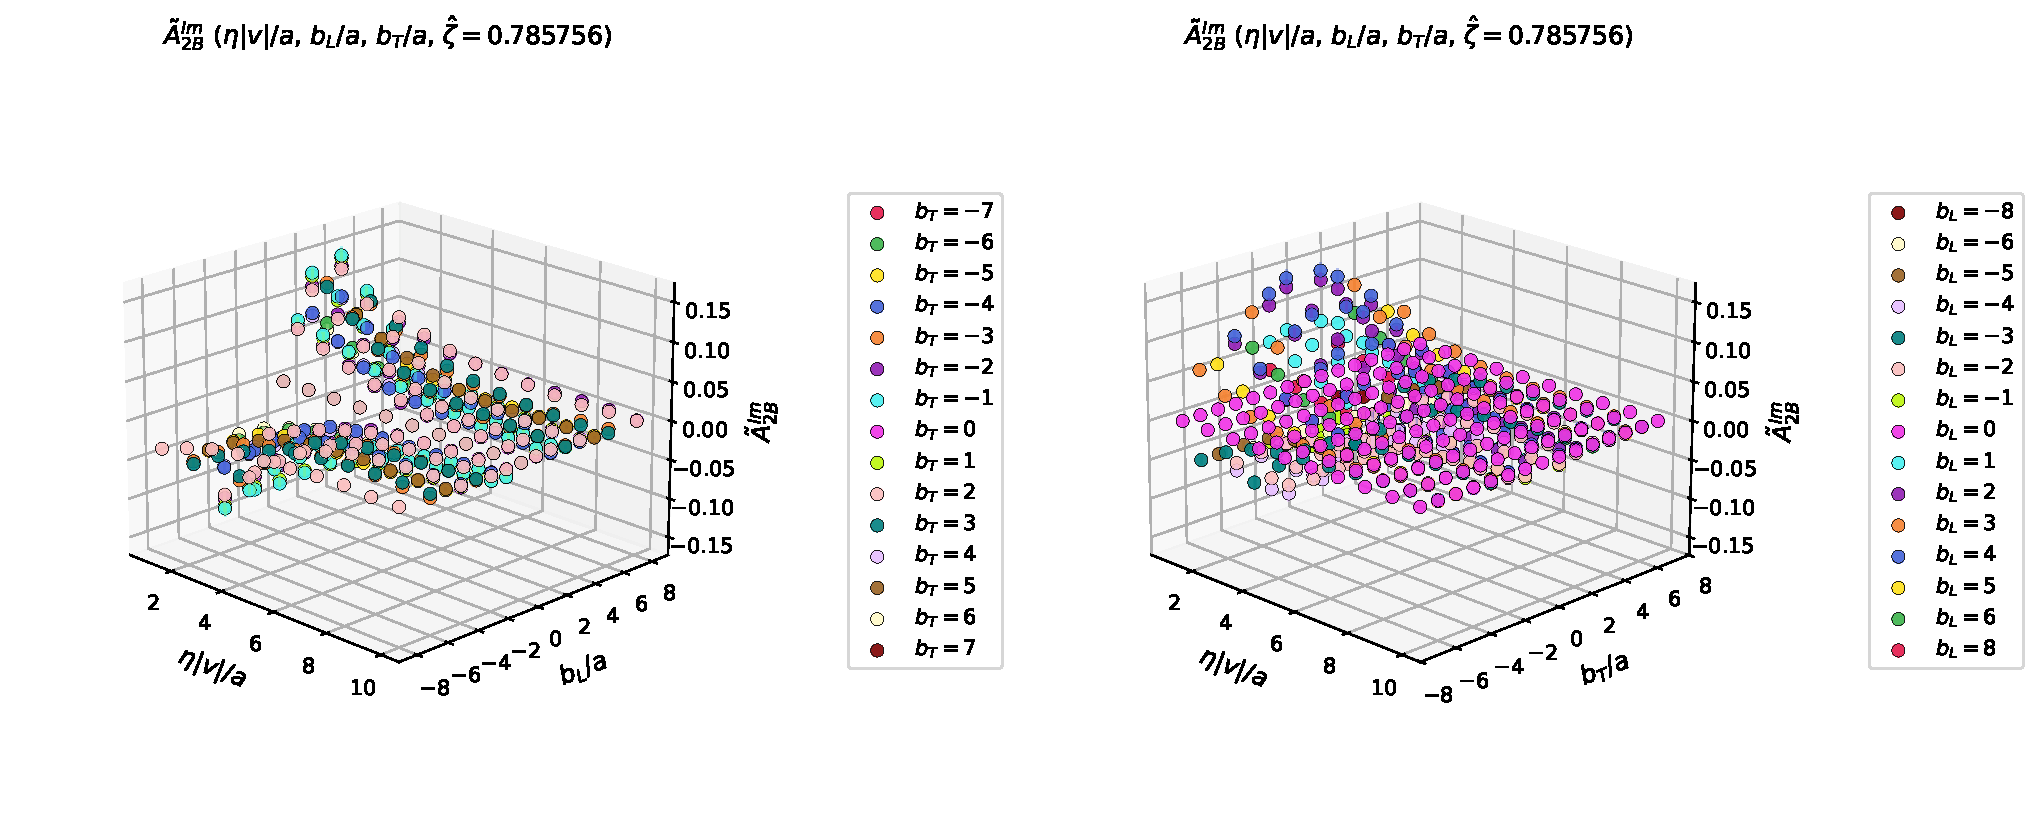
\includegraphics[width=0.7\linewidth]{plots/Amps_bL_bT/ImA2B_PL-4_3D.pdf}
    \caption{Caption}
    \label{fig:placeholder}
\end{figure}
\begin{figure}
    \centering
    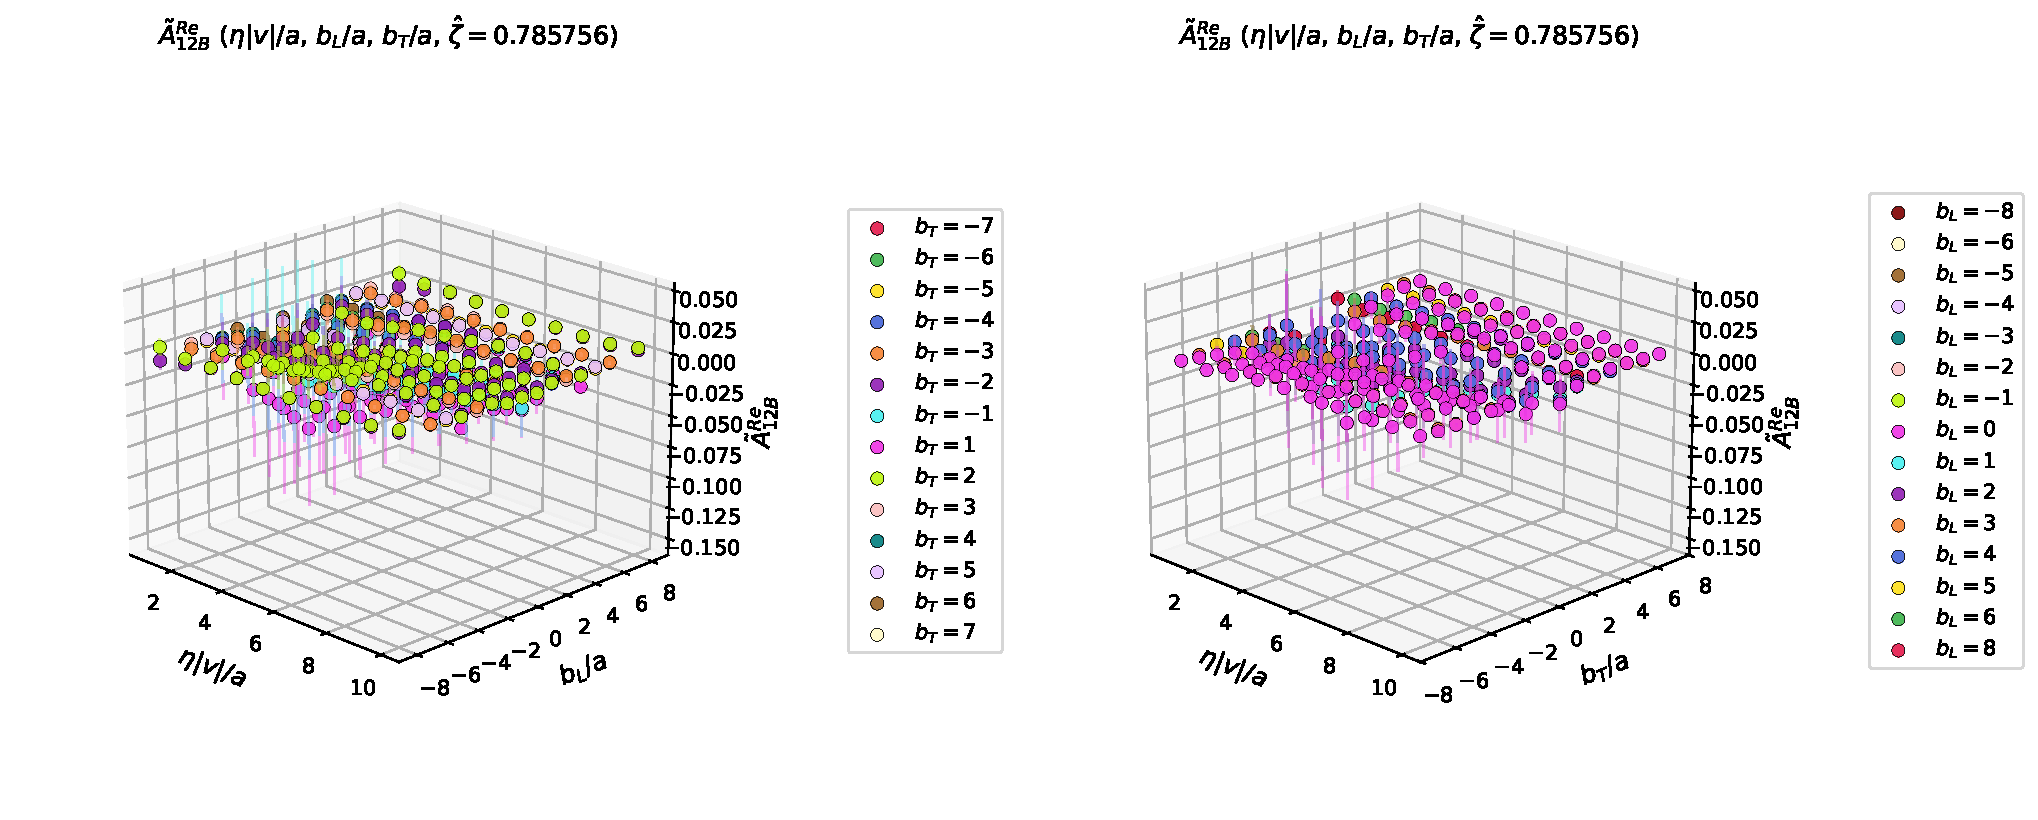
\includegraphics[width=0.7\linewidth]{plots/Amps_bL_bT/ReA12B_PL-4_3D.pdf}
    \caption{Caption}
    \label{fig:placeholder}
\end{figure}
\begin{figure}
    \centering
    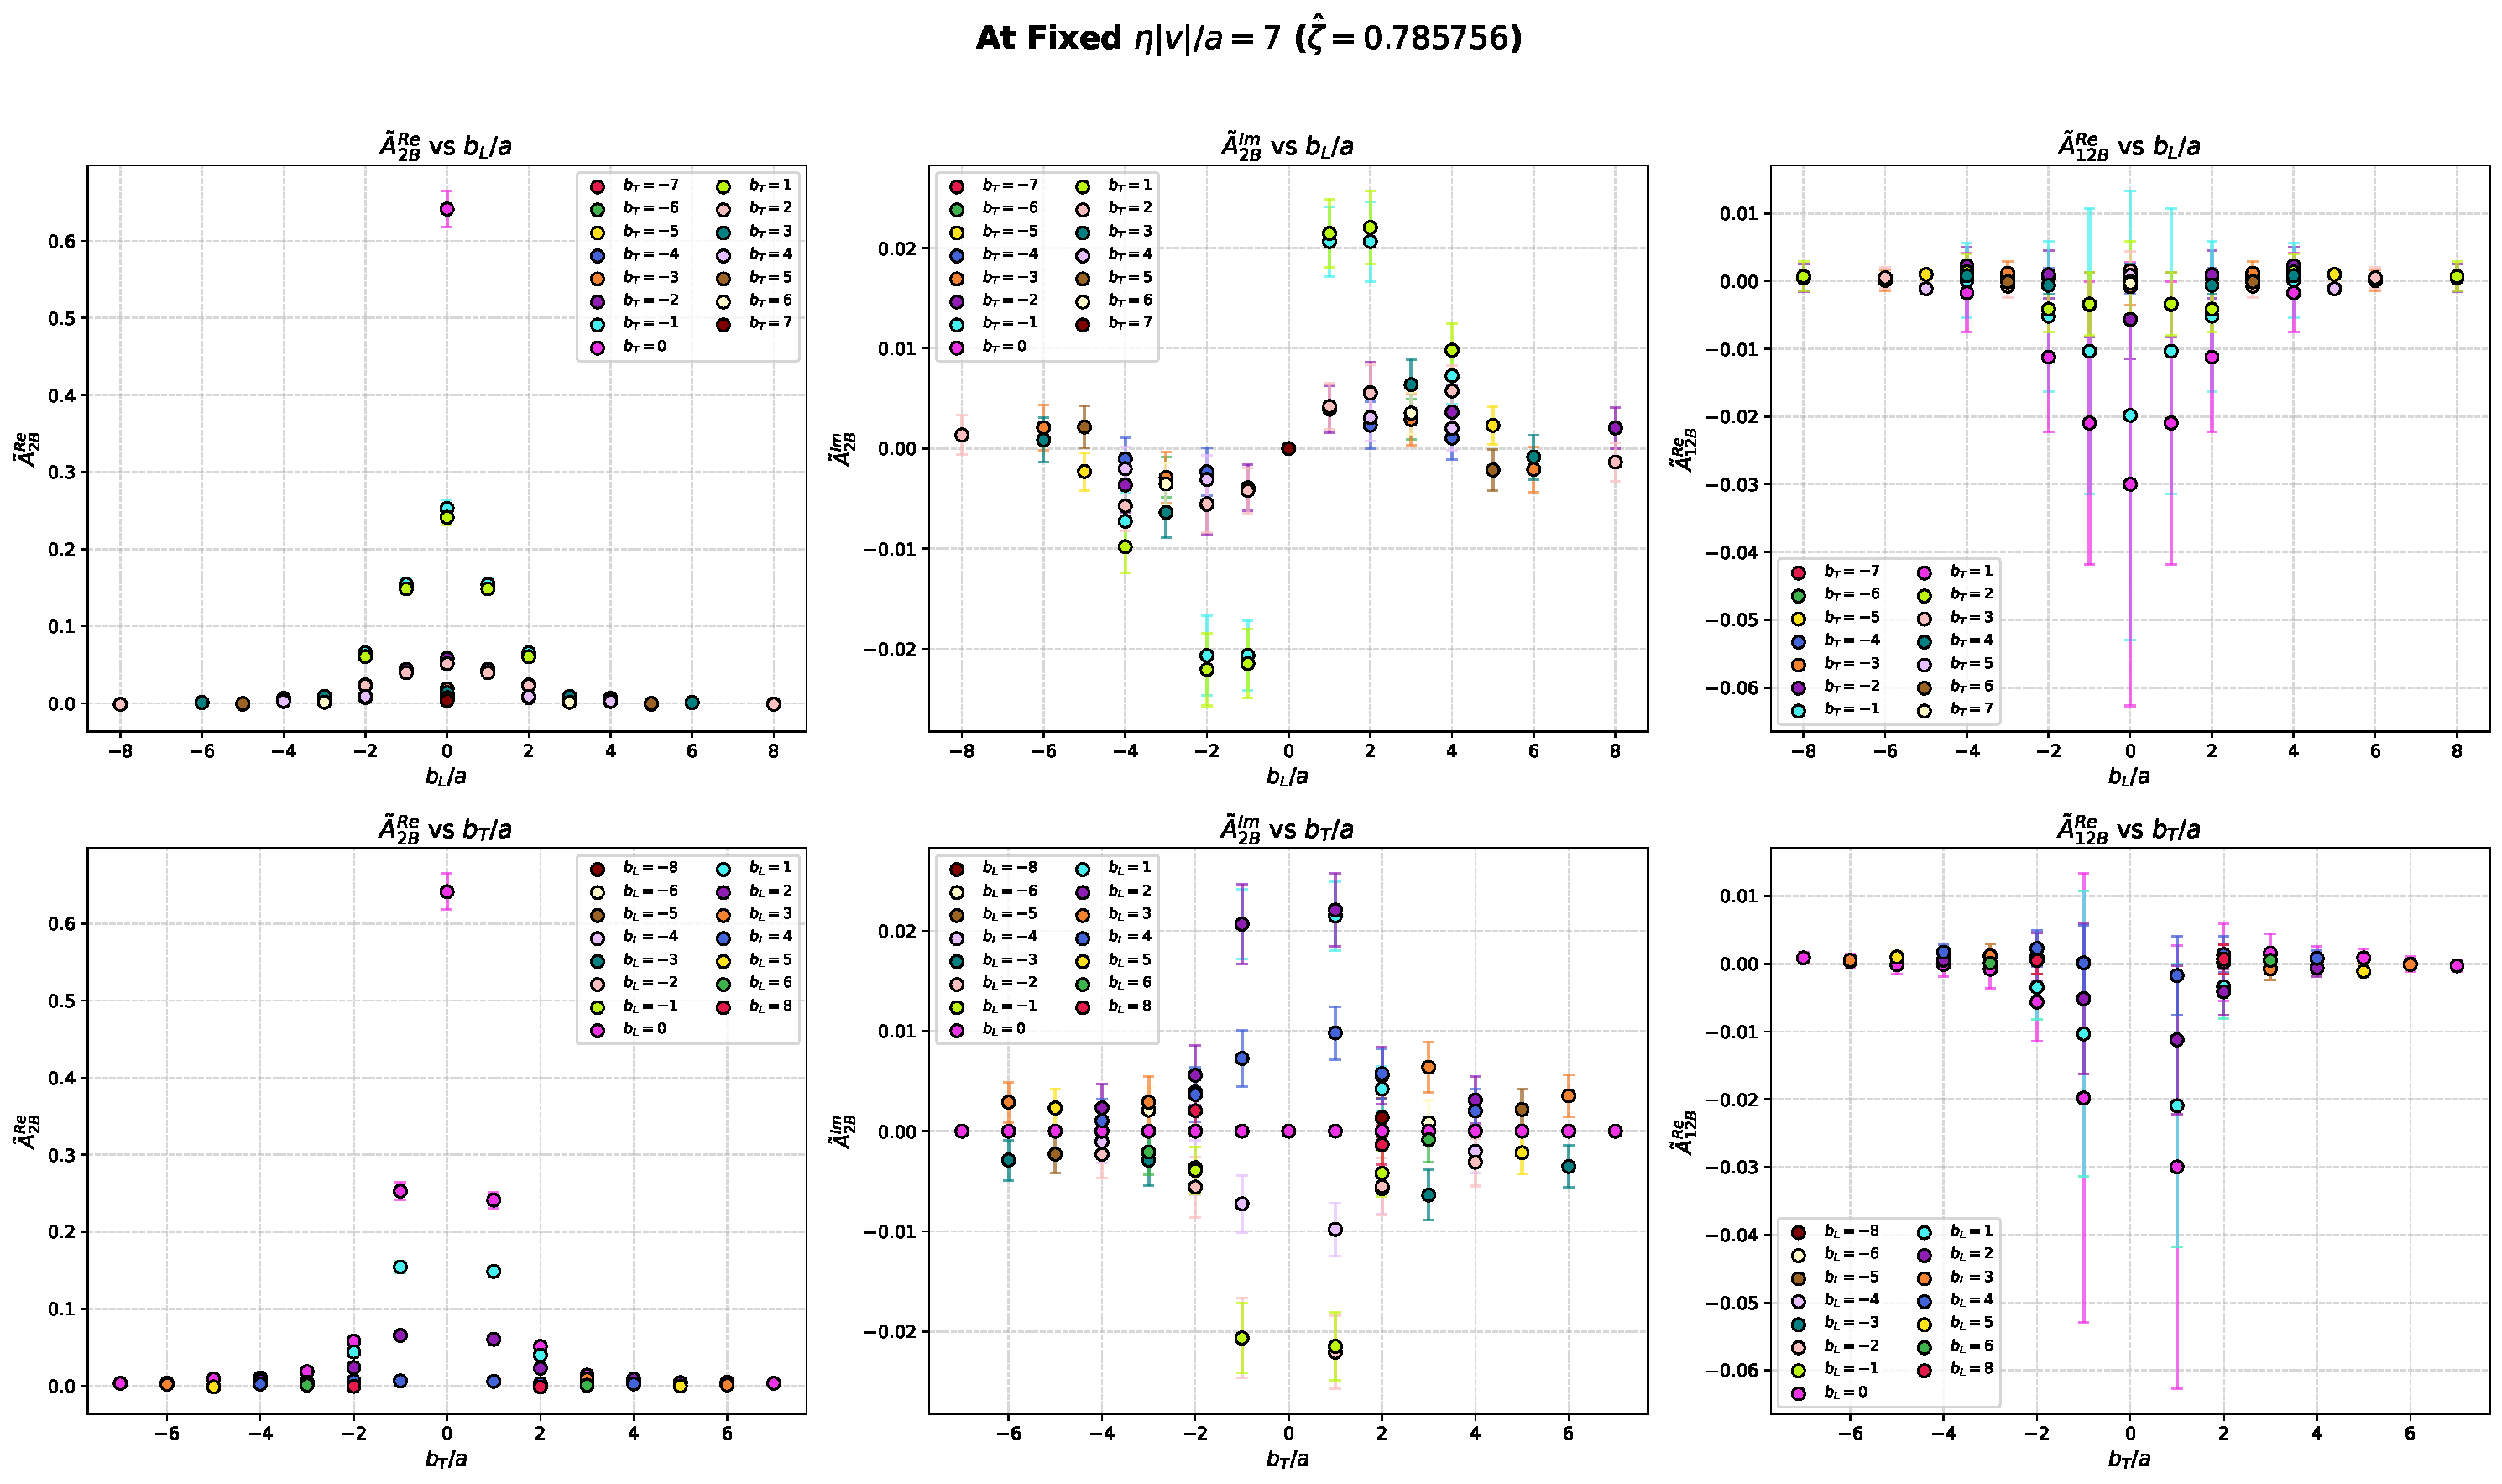
\includegraphics[width=0.7\linewidth]{plots/Amps_bL_bT/Combined_2D_eta7_PL-4.pdf}
    \caption{Caption}
    \label{fig:placeholder}
\end{figure}

\newpage
\section{FITTING METHODOLOGIES AND STABILITY ANALYSIS}
\label{sec:fitting_methodologies}

The lattice data show different levels of statistical precision among the invariant amplitudes. The real part of the unpolarized amplitude, $\tAmp_{2B}^{\text{Re}}$, has small statistical uncertainties across the simulated position space, whereas the imaginary unpolarized amplitude $\tAmp_{2B}^{\text{Im}}$ and the real Sivers amplitude $\tAmp_{12B}^{\text{Re}}$ have larger gauge noise. We already discarded the imaginary Sivers amplitude $\tAmp_{12B}^{\text{Im}}$ because it is consistent with zero. We first establish a stable global fit for $\tAmp_{2B}^{\text{Re}}$ as the baseline for the remaining numerical analysis, as it corresponds to the leading-twist unpolarized TMD and has the highest data quality.

We parameterize the amplitudes natively in the Cartesian space $(b_L, b_T)$ rather than the Lorentz-invariant variable space $(P \cdot b, b^2)$. Fitting in $(b_L, b_T)$ provides a larger, more uniformly distributed set of discrete data points and resolves kinematic degeneracies. Because the squared separation distance $b^2 = b_L^2 + b_T^2$ is strictly non-negative, multiple distinct combinations of longitudinal and transverse separations (such as a large $b_L$ with a small $b_T$, or a small $b_L$ with a large $b_T$) map to the same invariant $b^2$. So, fitting in the $(P \cdot b, b^2)$ basis would compress these distinct orthogonal spatial dependencies into a single coordinate. Fitting over the $(b_L, b_T)$ grid allows the model to separate the longitudinal decay profile from the transverse decay profile. 

The fitting and stability analysis in this chapter follows a sequential progression towards finding the final model. In Section~\ref {sec:gaussian_transformation}, we demonstrate why the simple Gaussian ansatz fails due to non-integrable longitudinal growth ($\alpha < \beta$). In Section~\ref{sec:discretization_effects}, we isolate ultraviolet lattice discretization artifacts by applying a spatial cutoff $|\vect{b}| \ge 3a$. In Section~\ref{sec:pysr_methodology}, using genetic programming with an asymptotic decay penalty, we discover the generalized Lorentzian power-law tail $(1+b^2)^{-j}$ and the exponential area-law factor $e^{-f\eta}$. In Sections~\ref{sec:rejection_exponential_longitudinal} and~\ref{sec:factorized_ansatze_failure}, We test factorized models across all three surviving amplitudes, showing that while they describe $\tAmp_{2B}^{\text{Re}}$, they fail on $\tAmp_{2B}^{\text{Im}}$ and $\tAmp_{12B}^{\text{Re}}$, requiring the coupled denominator $[1 + c(P\cdot b)^2/P_L^2 + d b^2]^j$. Then in Sections~\ref{sec:asymptotic_eta_anti_quark} and~\ref{sec:candidate_selection}, we analyze parameter behavior across individual staple extents $\eta \in [6, 10]$, select the asymptotic model $c(\eta) = c(1 - k_1/\eta - k_2/\eta^2)$ based on AIC, and enforce physical anti-quark suppression at large negative $x$ ($x < -0.2$). Finally, in Section~\ref{sec:simultaneous_fit_strategy}, we perform a correlated Jackknife $\chi^2$ minimization across all amplitudes, cancel the shared $e^{-f\eta}$ factor, and extract the $x$-dependent Sivers shift.

\subsection{Failure of Simple Gaussian Model}
\label{sec:gaussian_transformation}

For the real parts of the amplitudes ($\tAmp^{Re}_{iB}$), Hermitian conjugation symmetries require the function to be even in the longitudinal separation $b_L$. We model the real amplitude with a standard 2D Gaussian centered at the origin
\begin{align}
    \tAmp^{Re}_{iB}&=\gamma \exp{\left[-\alpha b_L^2-\beta b_T^2\right]}
\end{align}
To transform this into the invariant variable space, we use the lattice four-vector square, $b^2 = b_L^2 + b_T^2$, to substitute $b_T^2 = b^2 - b_L^2$ and also apply the Lorentz-invariant projection derived in Section \ref{sec:lorentz_mapping}, where the longitudinal spatial coordinate is given by $b_L = (P \cdot b) / (-P_L)$. Squaring this substitution gives
\begin{align}
   \tAmp^{Re}_{iB} &=\gamma \exp{\left[-\frac{\left(\alpha-\beta\right)}{P_{L}^2} (P\cdot b)^{2}-\beta b^{2}\right]}
\end{align}

For the Fourier integral $\int d(P\cdot b) e^{ix(P\cdot b)} \tAmp_{iB}$ to converge, the argument of the exponential must remain negative as $(P \cdot b) \to \pm \infty$. This requires $(\alpha - \beta) > 0$. If $\alpha < \beta$, the amplitude grows exponentially at large longitudinal separations, making the integral divergent.

Fitting this Gaussian model to our lattice data yields $\alpha < \beta$ for the unpolarized real amplitude, $\tAmp^{Re}_{2B}$. 
\begin{figure}[H]
    \centering
    % Left Column: Re A2B
    \begin{minipage}{0.48\textwidth}
        \centering
        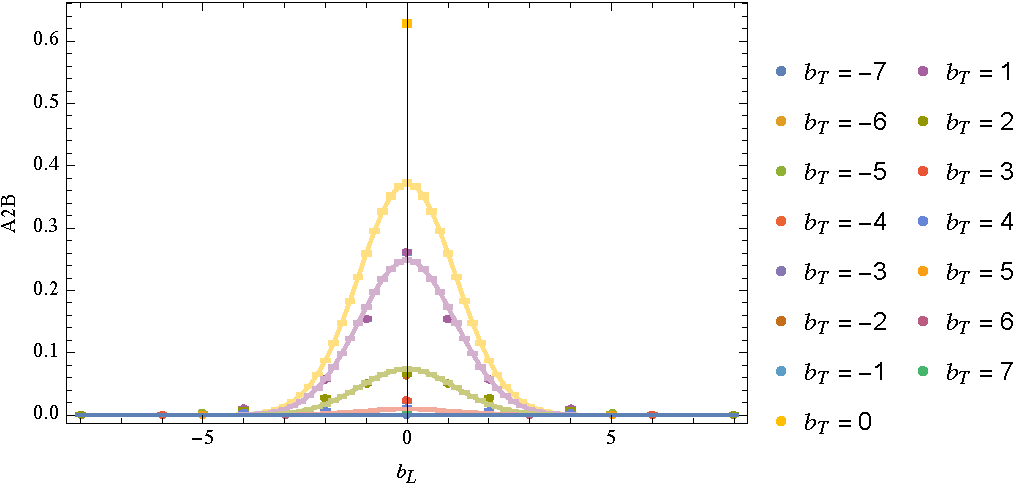
\includegraphics[width=\linewidth]{plots/Gaussian_fit_all_b/Gaussian_A2B_Re_P1_FailedFit.pdf}\\[2ex]
        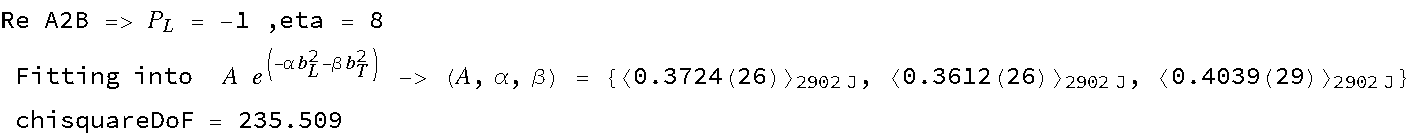
\includegraphics[width=\linewidth]{plots/Gaussian_fit_all_b/Gaussian_A2B_Re_P1_FailedFit_details1.pdf}\\[2ex]
        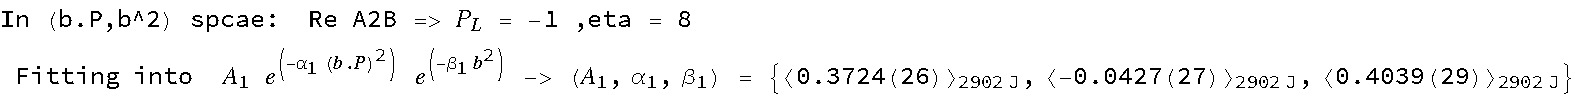
\includegraphics[width=\linewidth]{plots/Gaussian_fit_all_b/Gaussian_A2B_Re_P1_FailedFit_details2.pdf}
    \end{minipage}\hfill
    % Right Column: Re A12B
    \begin{minipage}{0.48\textwidth}
        \centering
        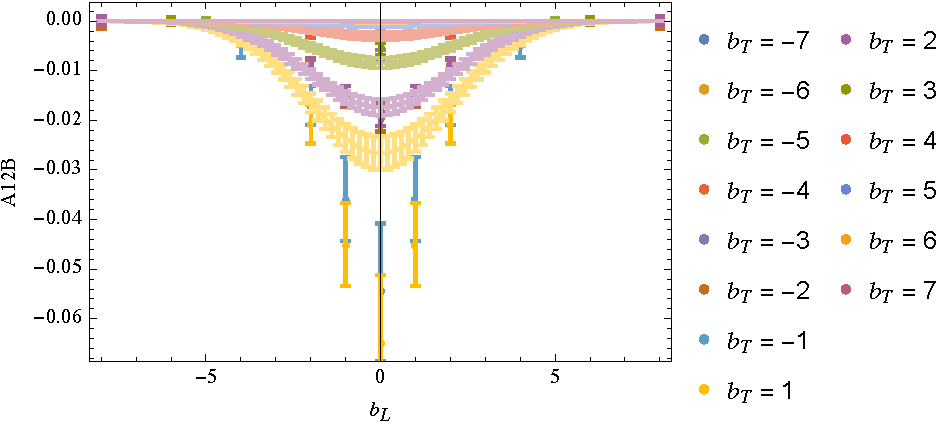
\includegraphics[width=\linewidth]{plots/Gaussian_fit_all_b/Gaussian_A12B_Re_P1_FailedFit.pdf}\\[2ex]
        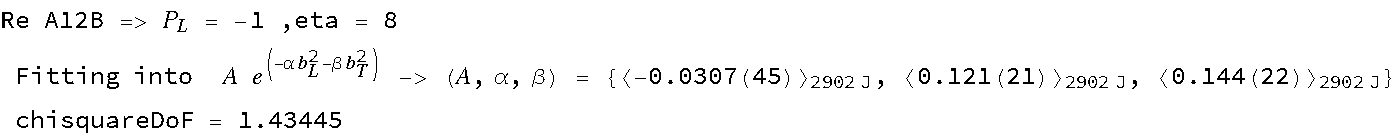
\includegraphics[width=\linewidth]{plots/Gaussian_fit_all_b/Gaussian_A12B_Re_P1_FailedFit_details1.pdf}\\[2ex]
        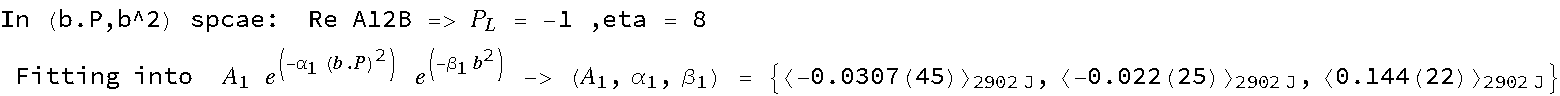
\includegraphics[width=\linewidth]{plots/Gaussian_fit_all_b/Gaussian_A12B_Re_P1_FailedFit_details2.pdf}
    \end{minipage}
    \caption{Failure of Gaussian model fit for $\tAmp^{Re}_{2B}$ (with $\alpha-\beta = -0.0427(27)$ and $\chi^2/\text{dof}\approx 235$) and $\tAmp^{Re}_{12B}$ (with $\alpha-\beta = -0.022(25)$ and $\chi^2/\text{dof}\approx 1.4$) amplitudes.}
    \label{fig:gaussian_failure}
\end{figure}

This means the amplitude decays faster in the transverse direction than in the longitudinal direction, leading to a non-integrable expansion in the $(P \cdot b, b^2)$ space. Additionally, the Gaussian model does not fit the data well, yielding a $\chi^2/\text{dof}\approx 230$. A symmetric 2D Gaussian decay profile is too rigid to describe the non-local operator. 

Because of this divergence and poor fit quality, we cannot use the simple Gaussian model. We instead use multi-parameter functions that accommodate distinct decay rates and guarantee convergence in the Fourier domain.


\subsection{Discretization Effects and Short-Distance Data Exclusion}
\label{sec:discretization_effects}

Before fitting the lattice amplitudes, we account for the limits of the discretized spacetime. Lattice QCD defines the theory on a discrete grid with a finite lattice spacing $a$. Observables evaluated at length scales comparable to $a$ contain discretization artifacts. At short quark-separation distances ($|\vect{b}| \sim 1a$ or $2a$), the continuous $O(4)$ rotational symmetry of Euclidean QCD breaks down to the discrete hypercubic group of the lattice. The step-wise Wilson lines connecting these closely spaced fields also introduce $\mathcal{O}(a)$ and $\mathcal{O}(a^2)$ finite-spacing errors. Fitting continuum models to these short-distance points would cause the algorithm to parameterize ultraviolet lattice artifacts instead of the non-perturbative structure of the nucleon.

To separate our parameterizations from these short-distance effects, we apply a spatial cut to our dataset before fitting. We exclude data points where the magnitude of the quark spatial separation is less than three lattice units:
\begin{equation}
    |\vect{b}| = \sqrt{b_L^2 + b_T^2} \ge 3a \ .
\end{equation}

With the dataset restricted to $b \ge 3a$, the non-local operator spans enough lattice sites for the step-wise gauge link to approach a continuous trajectory. This ensures the fitting algorithms and subsequent Fourier transforms depend on the long-range dynamics rather than the ultraviolet regulator.

\begin{figure}[H]
    \centering
    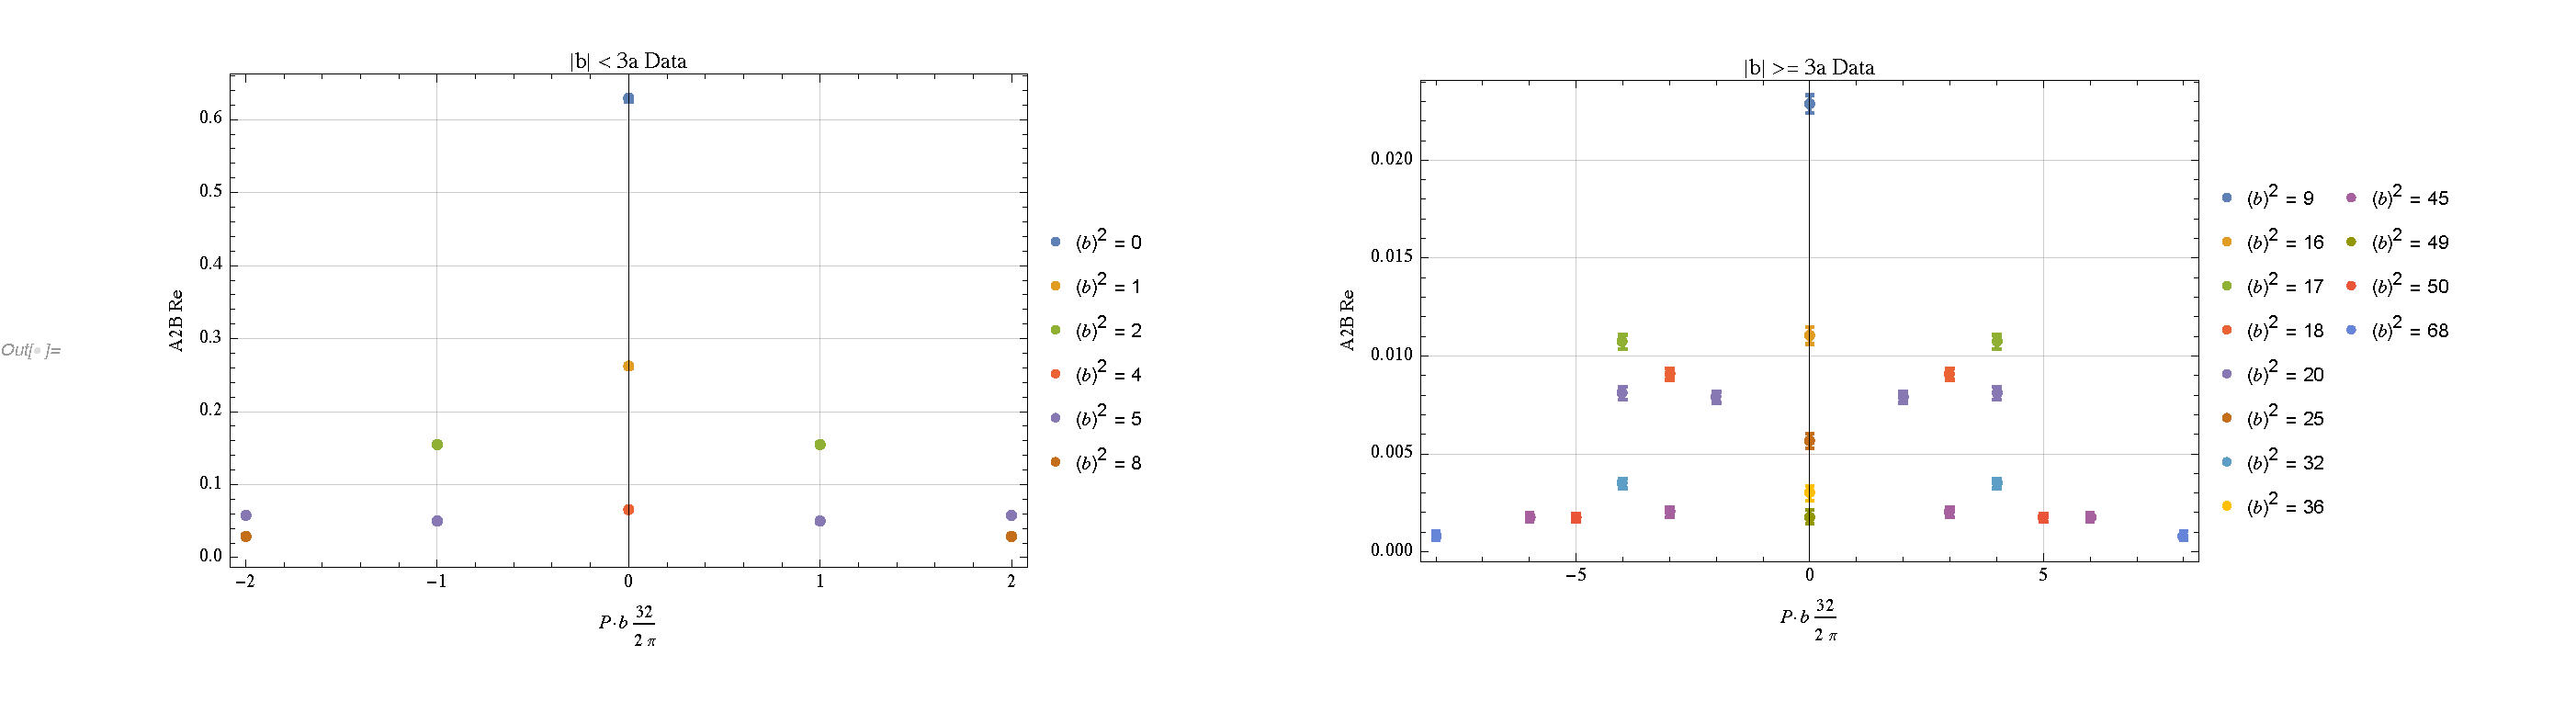
\includegraphics[width=1\linewidth]{plots/short_distance/A2B_Re_b_lessthan3_and_ge3.pdf}
    \caption{Plots of $\tAmp^{Re}_{2B}$ amplitude showing the short-distance data ($|\vect{b}| < 3a$) exhibiting an opposite curvature compared to the long-distance data ($|\vect{b}| \ge 3a$) for fixed momentum ($P=-1$) and fixed $\eta$ (say $\eta=8$)}
\end{figure}

\begin{figure}[H]
    \centering
    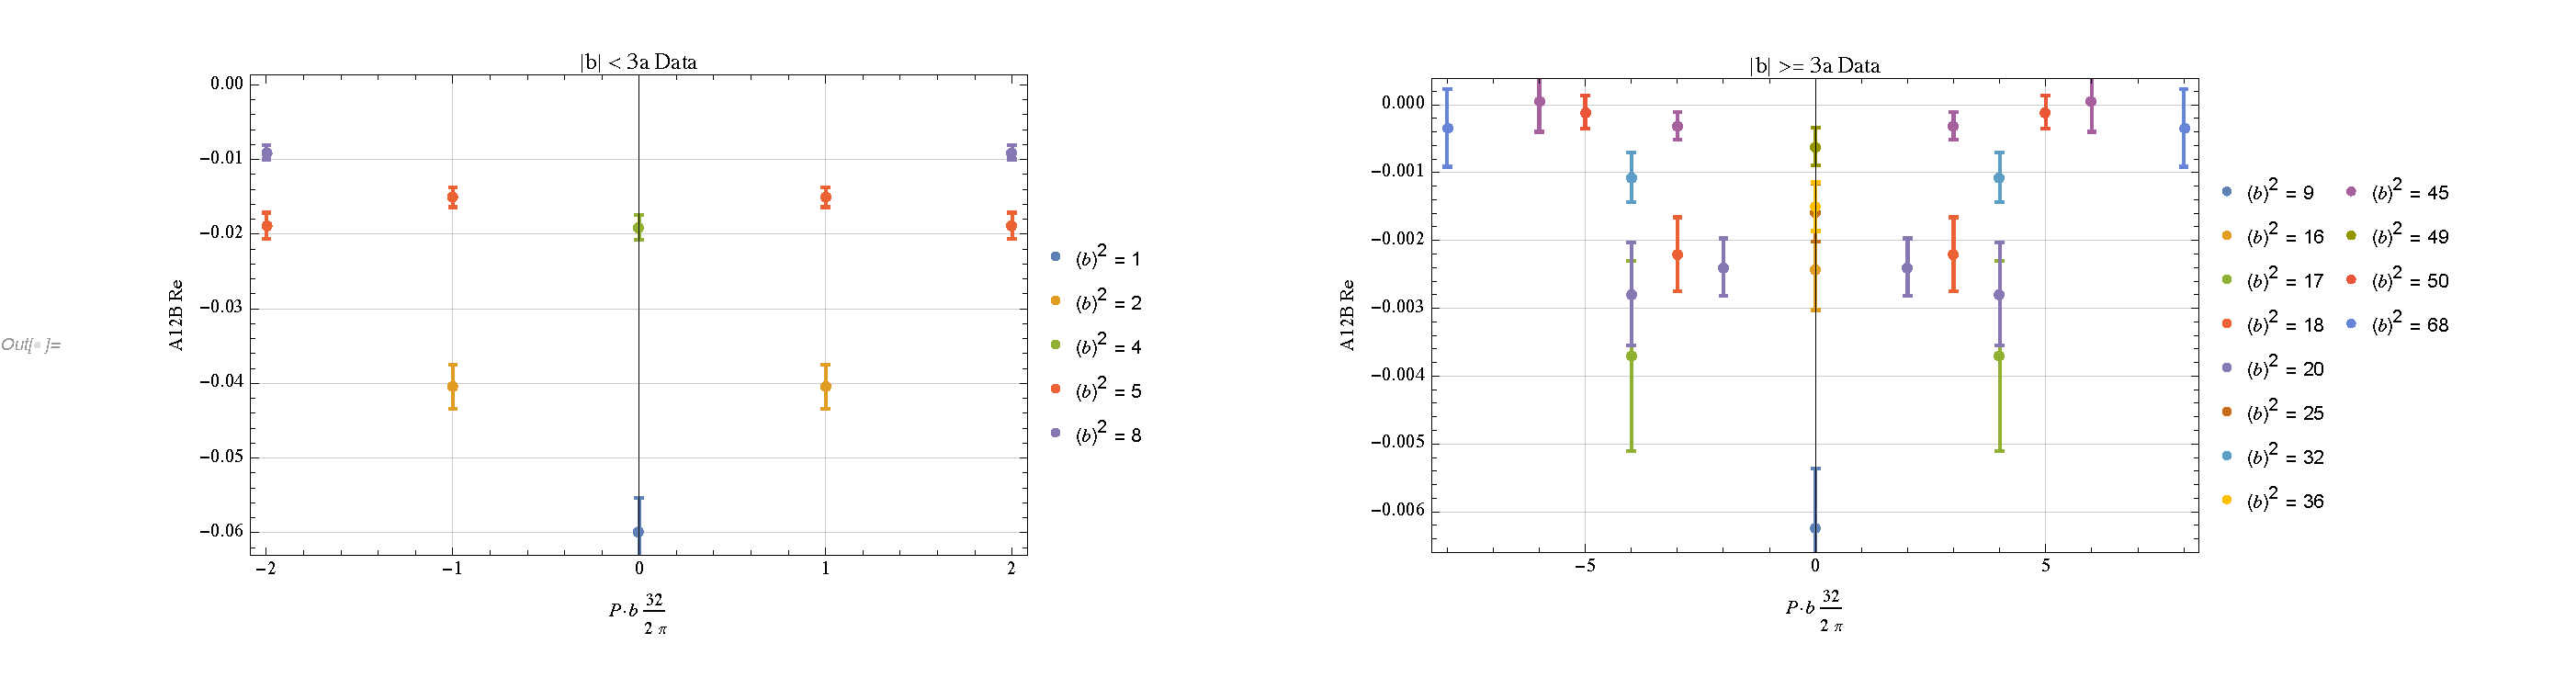
\includegraphics[width=1\linewidth]{plots/short_distance/A12B_Re_b_lessthan3_and_ge3.pdf}
    \caption{Plots of $\tAmp^{Re}_{12B}$ amplitude showing the short-distance data ($|\vect{b}| < 3a$) exhibiting an opposite curvature compared to the long-distance data ($|\vect{b}| \ge 3a$) for fixed momentum ($P=-1$) and fixed $\eta$ (say $\eta=8$)}
\end{figure}

All subsequent stability analyses, global fits, and extracted phenomenological parameters discussed in this chapter are derived strictly from this artifact-suppressed ($|\vect{b}| \ge 3a$) dataset.


\subsection{Physics-Informed Symbolic Regression via PySR}
\label{sec:pysr_methodology}

Selecting a multi-dimensional functional form by hand introduces human bias. To address this, we use Symbolic Regression (SR). 

Unlike traditional regression, which optimizes the parameters of a pre-determined function, symbolic regression searches the space of mathematical expressions and their parameters simultaneously. We utilize \texttt{PySR} \cite{Cranmer2023pysr}, a framework that uses Genetic Programming to discover interpretable equations from data by balancing accuracy and simplicity.

\subsubsection{Expression Search and Configuration}
\texttt{PySR} \cite{Cranmer2023pysr, Koza1992GP, Schmidt2009Distilling} uses a genetic algorithm to evolve mathematical expressions represented as binary trees iteratively. The algorithm evaluates a population of expressions against the lattice data using a custom loss function over thousands of generations. 

Table~\ref {tab: pysr_config} details the \texttt{PySR} search configuration, including the permitted mathematical operators, nesting constraints, and key hyperparameters. The operator library includes a custom Lorentzian-type binary operator, $\text{lor}(x, y) = 1/(1 + x^2 + y^2)^2$, alongside standard arithmetic and exponential functions. At the same time, nesting constraints prevent the algorithm from generating physically meaningless double-exponential or double-decay structures.

\input{PySR_outputs/pysr_model_config}


\subsubsection{The Physics-Informed Custom Loss Function}

Standard symbolic regression optimizes metrics like Mean Squared Error (MSE). However, a genetic algorithm might discover a polynomial or diverging exponential function that fits the finite $(b_L, b_T)$ lattice grid well, but diverges as $b_L \to \infty$. As shown in Section \ref{sec:gaussian_transformation}, this would cause the subsequent Fourier transform over $P \cdot b$ to diverge.

We implemented a custom loss function within \texttt{PySR} to enforce the required asymptotic decay. The reduced chi-squared statistic determines the base accuracy of the model:
\begin{align}
    \mathcal{L}_{\text{base}} = \frac{\chi^2}{\text{dof}} = \frac{1}{N - k} \sum_{i=1}^{N} \left( \frac{\tAmp_{2B}^{\text{Re, lattice}}(i) - \tAmp_{2B}^{\text{Re, model}}(i)}{\sigma_i} \right)^2
\end{align}

Here, $N$ is the number of lattice data points, $k$ is the number of degrees of freedom in the generated expression, and $\sigma_i$ is the statistical error of the $i$-th lattice point.

To enforce the asymptotic decay required for Fourier integrability, we introduce a penalty term. We evaluate the proposed model equation at large values of the longitudinal separation, $b_L^{\text{large}}$, while keeping the transverse separations $b_T$ fixed to physical slices. We compute the sum of the absolute model predictions in this asymptotic regime:
\begin{align}
    \mathcal{P}_{\text{asymptotic}} = \sum_{b_T \in \{b_{T}^{\text{fixed}}\}} \sum_{b_L \in \{b_{L}^{\text{large}}\}} \left| \tAmp_{2B}^{\text{Re, model}}(b_L, b_T) \right|
\end{align}

If a generated equation diverges or grows at large $b_L$, the penalty term $\mathcal{P}_{\text{asymptotic}}$ increases, lowering the equation's fitness score. If the equation decays toward zero, the penalty vanishes.

We combine these terms into the total objective function for \texttt{PySR}. The penalty is scaled by a small regularization parameter $\epsilon$:
\begin{align}
    \mathcal{L}_{\text{custom}} &= \mathcal{L}_{\text{base}} + \epsilon \, \mathcal{P}_{\text{asymptotic}} \\
    \mathcal{L}_{\text{custom}} &= \frac{\chi^2}{\text{dof}} + \epsilon \sum_{b_T \in \{b_{T}^{\text{fixed}}\}} \sum_{b_L \in \{b_{L}^{\text{large}}\}} \left| \tAmp_{2B}^{\text{Re, model}}(b_L, b_T) \right|
\end{align}

By evaluating fitness using $\mathcal{L}_{\text{custom}}$, \texttt{PySR} restricts the search to mathematical expressions that fit the finite lattice data and obey the asymptotic decay constraints. The Julia implementation of this objective function is shown below. The asymptotic penalty evaluates each candidate expression at five test coordinates in the regime $b_L \gg 1$, spanning staple extents $\eta \in \{6, 8, 10\}$ and longitudinal separations up to $b_L = 80a$. We set the regularization weight to $\epsilon = 0.1$.

\input{PySR_outputs/pysr_custom_loss_code}

\subsubsection{Pareto Front of Discovered Models}

Symbolic regression outputs a Pareto front of candidate models: a ranked list of equations that trade off mathematical simplicity (measured by expression tree complexity $C$) and predictive accuracy (measured by the custom loss $\mathcal{L}_{\text{custom}}$). The Pareto front for the real unpolarized amplitude $\tAmp_{2B}^{\text{Re}}$ is presented in Table~\ref{tab:pysr_pareto_front}.

\input{PySR_outputs/pysr_equations_table}

At the lowest complexities ($C \leq 4$), \texttt{PySR} isolates the overall $\eta$-dependence of the amplitude as an exponential decay $\sim (0.499)^\eta \approx e^{-0.695\eta}$, consistent with the area-law suppression of the extended Wilson line. At intermediate complexities ($C = 7$--$12$), the algorithm introduces spatial $b$-dependence through Lorentzian-type power-law denominators $(1 + b_L^2 + b_T^2)^{-j}$ alongside linear or power-law $\eta$-models. The algorithm does not select a Gaussian spatial profile $e^{-cb^2}$ at any point along the Pareto front. It instead converges on the power-law tail structure, aligning with the findings in Section~\ref{sec:gaussian_transformation}.

The models at complexities $C = 14$ and $C = 16$ best balance accuracy and structure. The $C = 14$ expression achieves a factorized form:
\begin{equation}
    \tAmp_{2B}^{\text{Re}} = \frac{39.71}{(1 + b_L^2 + b_T^2)^{1.39}} \, e^{-0.534\eta} \ ,
    \label{eq:pysr_C14}
\end{equation}
which is a product of an exponential decay in $\eta$ and a generalized Lorentzian power-law decay in $b^2 = b_L^2 + b_T^2$. The $C = 16$ model introduces a small additive constant offset of $-0.00127$, reducing the loss to $\mathcal{L}_{\text{custom}} = 2.03$:
\begin{equation}
    \tAmp_{2B}^{\text{Re}} = \frac{245.5}{(1 + b_L^2 + b_T^2)^{1.26}} \, e^{-0.468\eta} - 0.00127 \ .
    \label{eq:pysr_C16}
\end{equation}
Beyond $C = 16$, added complexity yields marginal loss improvements while reducing interpretability.

The power-law tail $(1 + b^2)^{-j}$ with $j > 1/2$ decays algebraically at large separations. This decays more slowly than a Gaussian but remains absolutely integrable over the real line. Unlike the Gaussian model, where the sign of $(\alpha - \beta)$ can render the Fourier integral divergent, the power-law denominator guarantees convergent integrals for positive exponents $j > 1/2$. The factorized structure $e^{-f\eta} \times g(b^2)$ also allows the shared $\eta$-dependent exponential to cancel analytically in the Sivers shift ratio, which we use in Section~\ref{sec:simultaneous_fit_strategy}.

\begin{figure}[htbp]
    \centering
    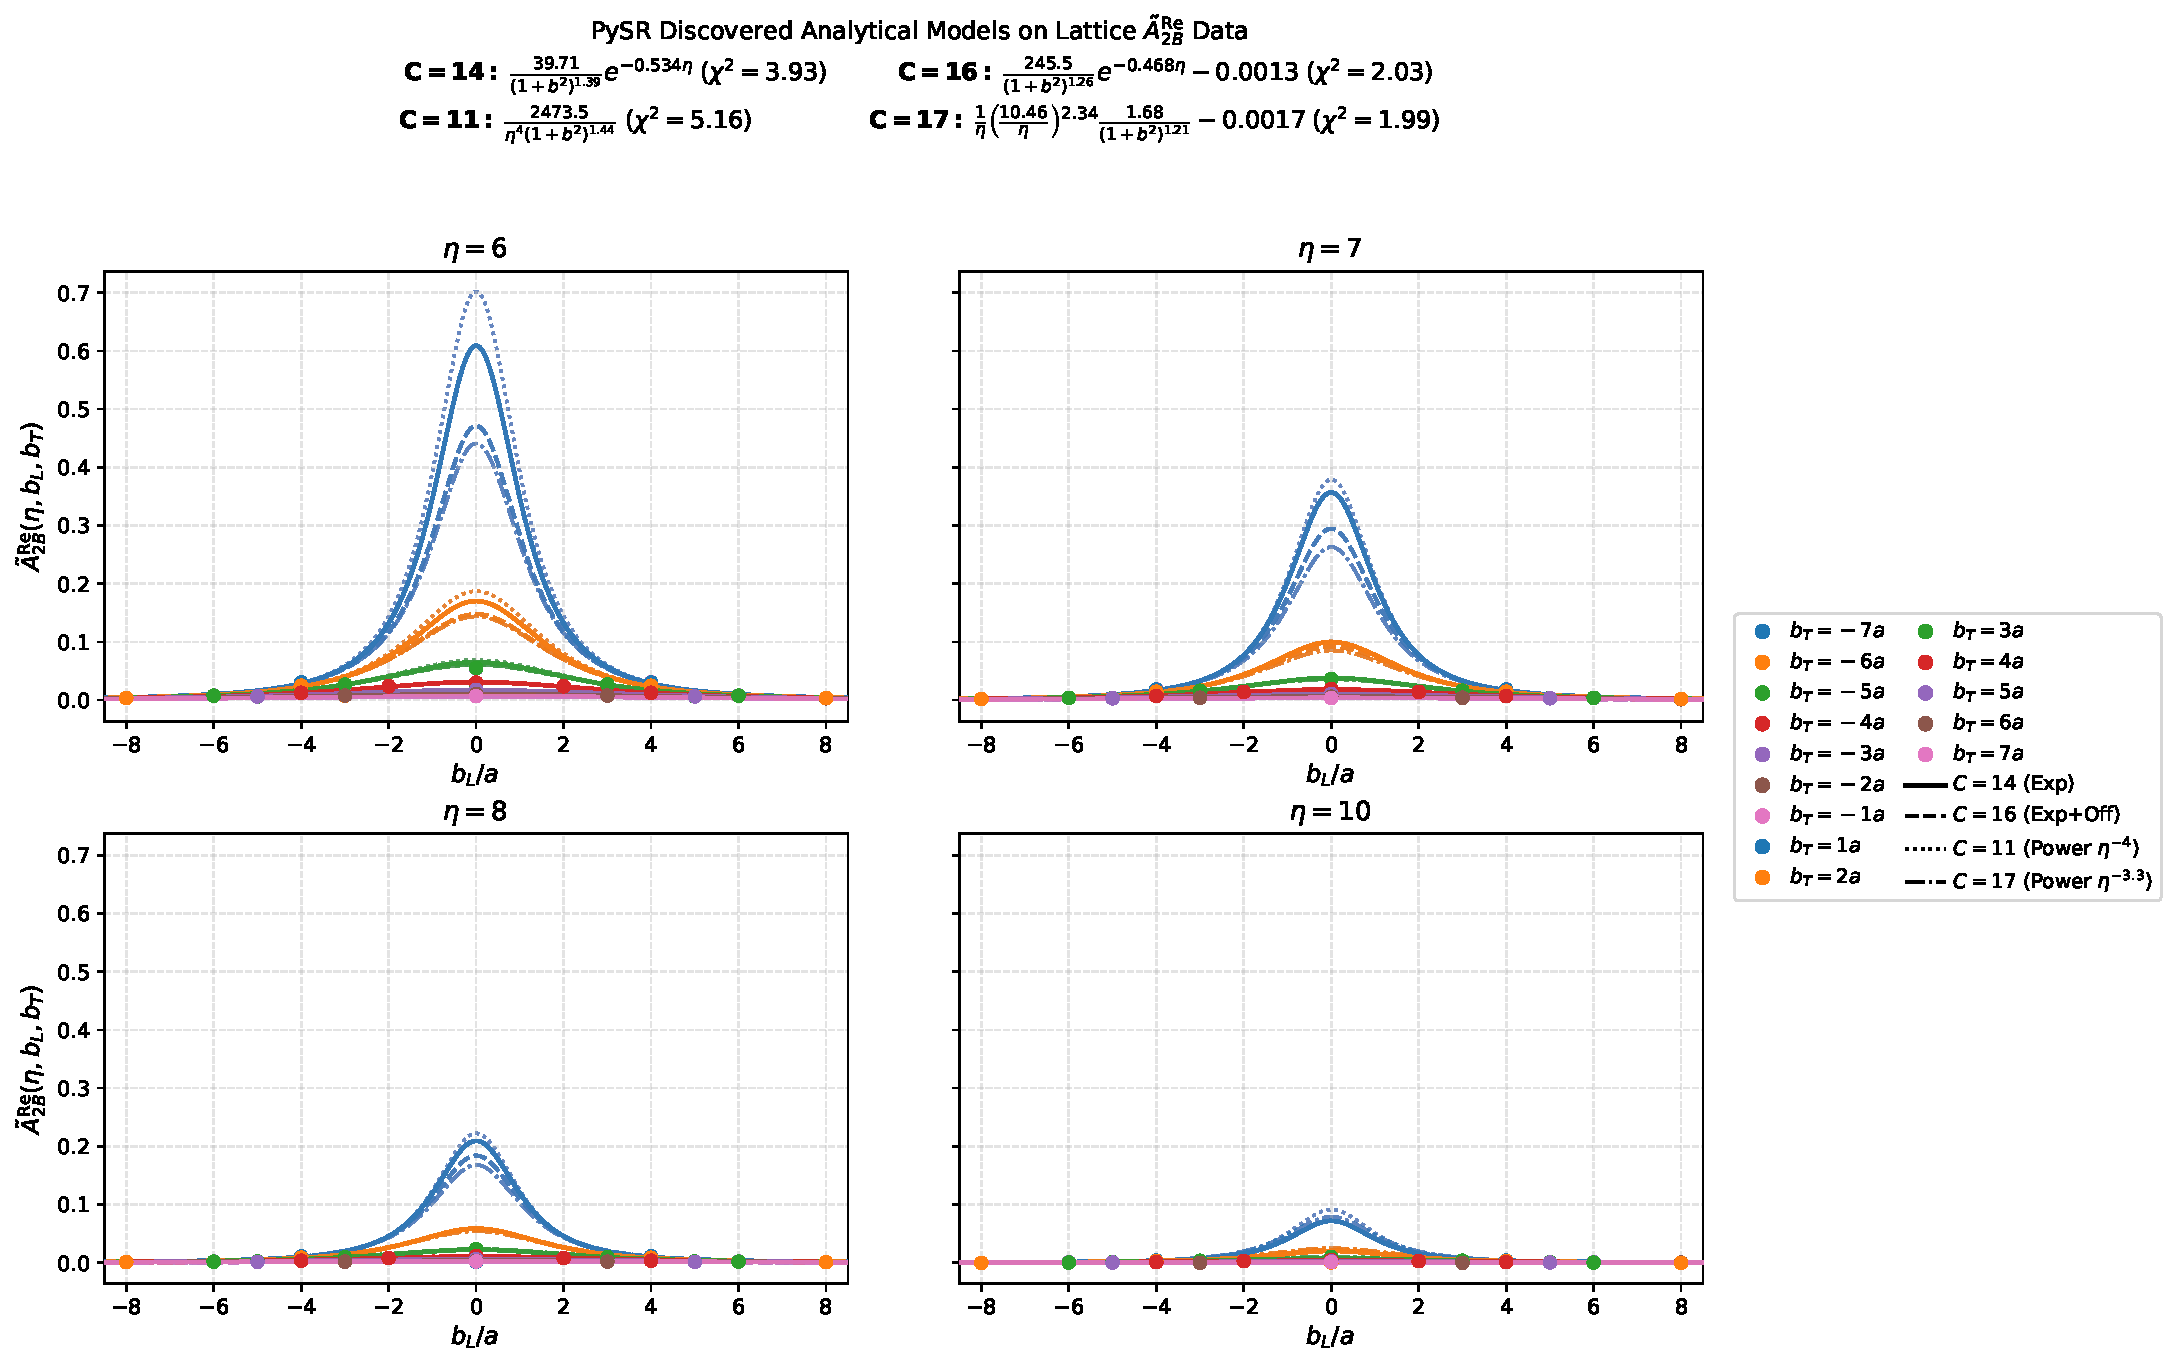
\includegraphics[width=1\linewidth]{PySR_outputs/01_A2B_PySR_Benchmark_Fits.pdf}
    \caption{Multi-panel comparison of the top \texttt{PySR}-discovered analytical models ($C = 11, 14, 16, 17$) against the lattice data for $\tAmp_{2B}^{\text{Re}}$ at fixed staple extents $\eta = 6, 7, 8, 10$ (with $P_1 = -1$ and $|\vect{b}| \geq 3a$). Each panel displays the amplitude as a function of the longitudinal separation $b_L/a$ at fixed transverse separations $b_T$, with the four Pareto-front models overlaid. The two exponential-$\eta$ models ($C = 14$, solid; $C = 16$, dashed) provide the most balanced description across all $\eta$ values, while the pure power-law-$\eta$ models ($C = 11$, dotted; $C = 17$, dot-dashed) exhibit slight systematic deviations at the extremes of the $\eta$ range.}
    \label{fig:pysr_benchmark_fits}
\end{figure}

\begin{figure}[htbp]
    \centering
    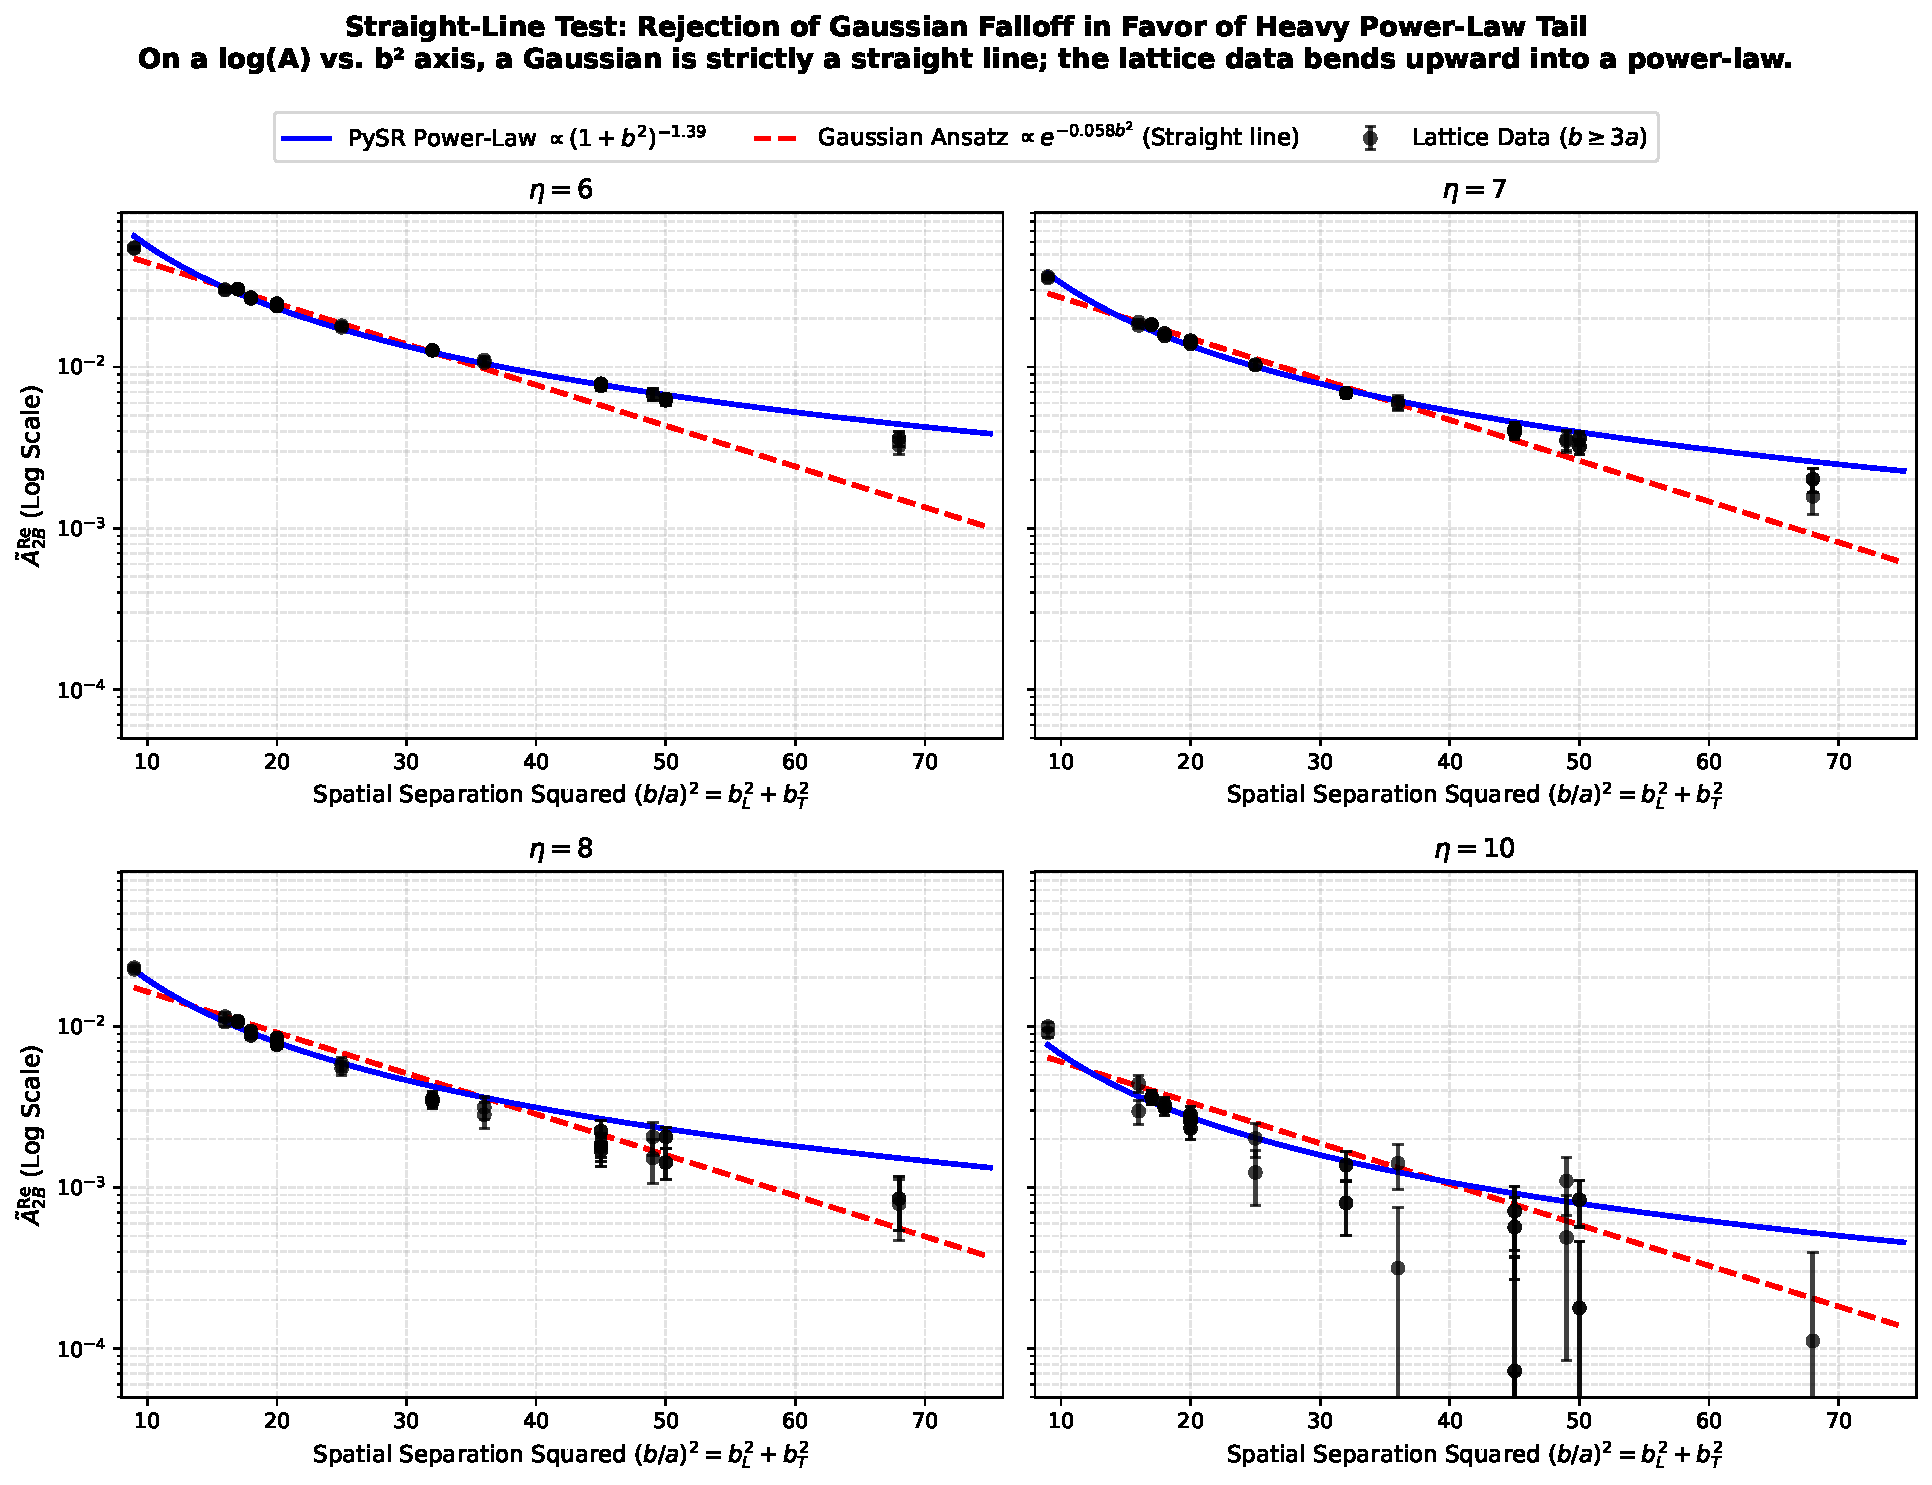
\includegraphics[width=0.95\linewidth]{PySR_outputs/02_Gaussian_StraightLine_Test.pdf}
    \caption{Diagnostic straight-line test for the Gaussian hypothesis. If the amplitude followed a pure Gaussian profile $\tAmp_{2B}^{\text{Re}} \propto e^{-c\,b^2}$, the data would appear as a straight line on a logarithmic ordinate versus $b^2$ (red dashed line, optimal Gaussian fit with $c = 0.058$). The lattice data (black markers) exhibit clear upward curvature away from the Gaussian baseline at large $b^2$, indicating a heavier-than-Gaussian tail that is accurately captured by the \texttt{PySR}-discovered power-law form $(1 + b^2)^{-1.39}$ (blue solid line). This provides direct, model-independent evidence that the spatial decay of the non-local quark bilinear follows an algebraic power law rather than a Gaussian exponential.}
    \label{fig:gaussian_straightline_test}
\end{figure}

As shown in Fig.~\ref{fig:pysr_benchmark_fits}, the factorized $C = 14$ and $C = 16$ expressions track the lattice data throughout the accessible $(b_L, b_T)$ grid across all staple extents. The pure power-law-$\eta$ models ($C = 11, 17$) exhibit slight systematic tension at the boundary $\eta$ values, where their $\eta^{-n}$ dependence departs from the exponential decay.

The straight-line diagnostic in Fig.~\ref{fig:gaussian_straightline_test} tests the Gaussian hypothesis. If the amplitude followed a Gaussian decay, plotting $\tAmp_{2B}^{\text{Re}}$ on a logarithmic ordinate against $b^2$ would yield a straight line with slope $-c$. The lattice data shows upward curvature at large $b^2$, indicating that the amplitude decays more slowly than an exponential. This behavior matches the generalized Lorentzian power-law tail discovered by the genetic algorithm.

Based on these results, we adopt the Lorentzian power-law structure as the spatial profile for $\tAmp_{2B}^{\text{Re}}$. In the following sections, we extend this functional form to the remaining amplitudes for the global simultaneous fit.

\subsection{Test for Factorization in $(P\cdot b)$ and $b^2$} \label{Test-for-Factorization}

To probe, directly at the level of the raw lattice data and independent of any fitted parameterization, whether the extracted amplitude factorizes as $\tAmp(P\cdot b,b^2) = F(P\cdot b) G(b^2)$, we performed a ratio test at fixed $P\cdot b$, which has multiple $b^2$, for example $b^2_1,b^2_2, b^2_3$, at the given momentum $P_L$. We formed
$$
R(b^2_i) = \frac{\tAmp(P\cdot b, b^2_i)}{\tAmp(P\cdot b, b^2_3)}
$$

\begin{figure}[htbp]
    \centering
    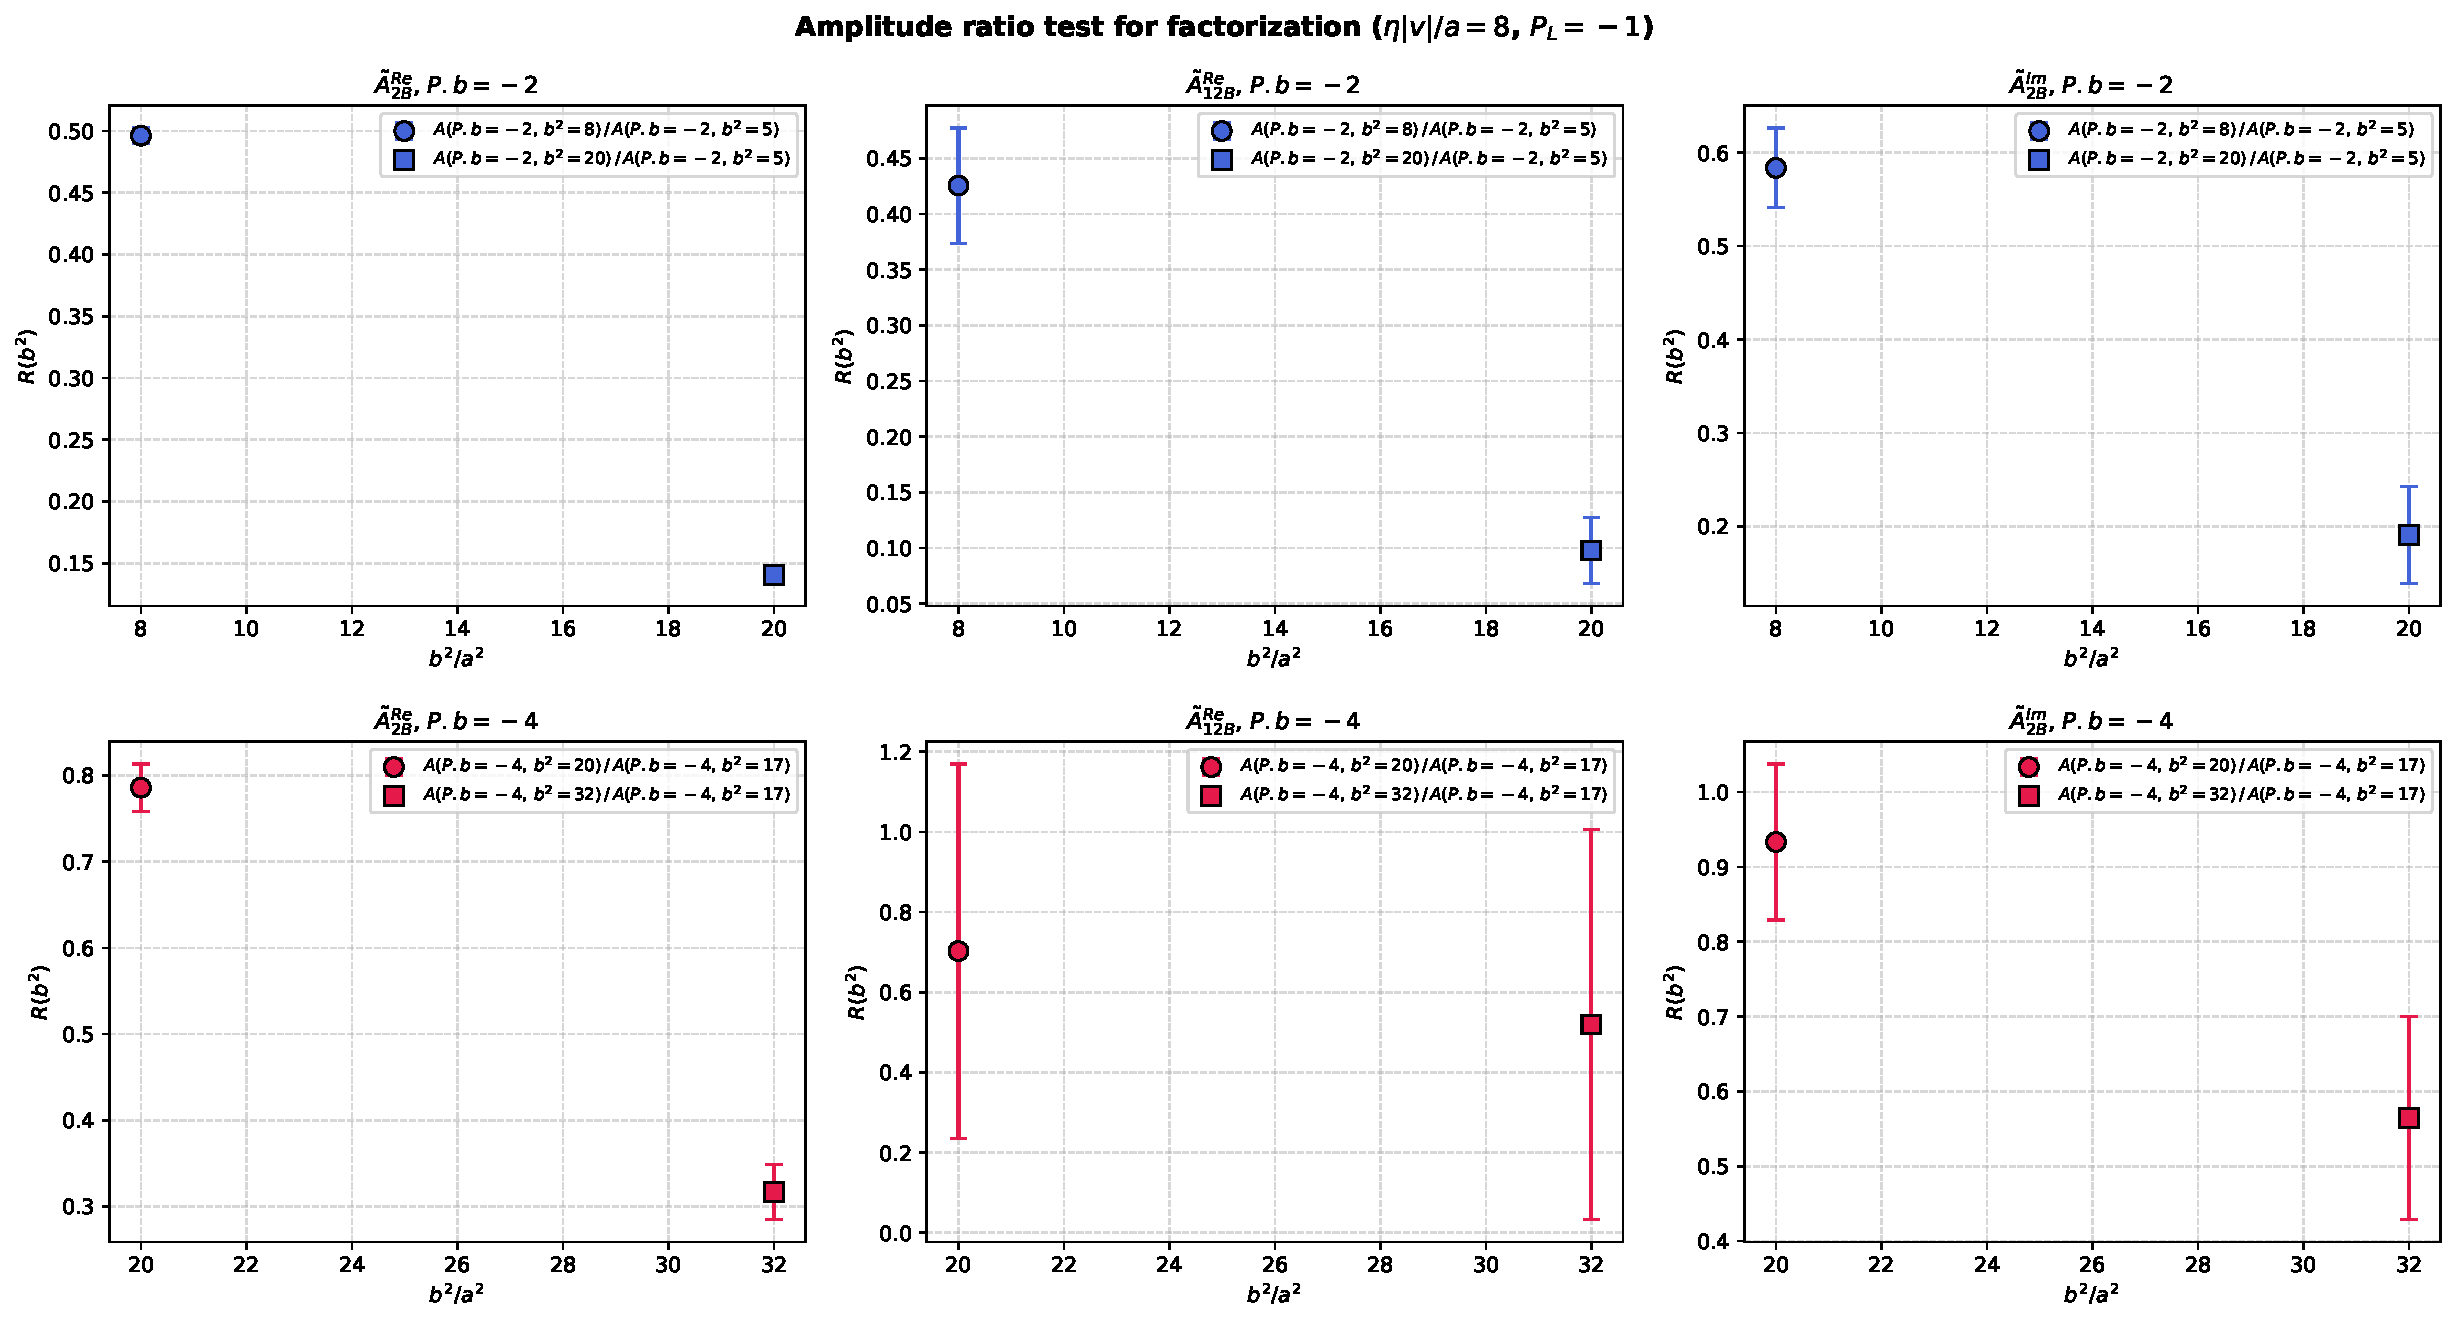
\includegraphics[width=1\linewidth]{plots/FixedPb_Bsq_RatioTest_eta8_PL-1.pdf}
    \caption{Ratio test for $(P\cdot b,b^2)$ factorization at fixed $P\cdot b$, for $\tAmp_{2B}^{\rm Re}$, $\tAmp_{12B}^{\rm Re}$, and $\tAmp_{2B}^{\rm Im}$ at $\eta|v|/a=8$, $P_L=-1$. Top row: $P\cdot b=-2$; bottom row: $P\cdot b=-4$; each point is ratioed against that row's own smallest available $b^2$, with the explicit ratio given in the legend.}
    \label{fig:FixedPb_Bsq_RatioTest_eta8_PL-1}
\end{figure}

The two rows in Fig.~\ref{fig:FixedPb_Bsq_RatioTest_eta8_PL-1} do not trace a common zero-slope line in $b^2$, as a factorized ansatz would predict. A fully model-independent version of this test would additionally require ratioing at fixed $b^2$ between different values of $P\cdot b$; however, the $(b_L,b_T)$ points computed on the lattice do not form a regular grid in $(P\cdot b,b^2)$, and at most two distinct $P\cdot b$ values ever coincide at a common $b^2$ anywhere in the dataset, with no two $P\cdot b$ rows sharing two or more common $b^2$ values. This limited sampling prevents us from carrying out the complementary ratio test at fixed $b^2$. Given this limitation, while the data appears to disfavor an exactly factorized ansatz, we treat this observation only as a qualitative guide rather than a firm conclusion. In the next section, we instead explore a fit model built directly on a factorized ansatz along with several non-factorized ansatze.



\subsection{Systematical exploration of the best physical model}
Based on the \texttt{PySR} analysis, we started exploring numerous power-law models for $\tAmp_{2B}^{\text{Re}}$ for momentum $P_L=-1$, $6\leq\eta\leq10$, and $b\geq3$. For completeness, we started with a Gaussian model and introduced several $\eta$-dependent ans\"atzes. For each model, the table lists the model expression, the list of fit parameters, the jackknife-averaged fitted values with statistical uncertainties, and the resulting $\chi^2/\mathrm{DoF}$.
\begin{figure}[htbp]
    \centering
    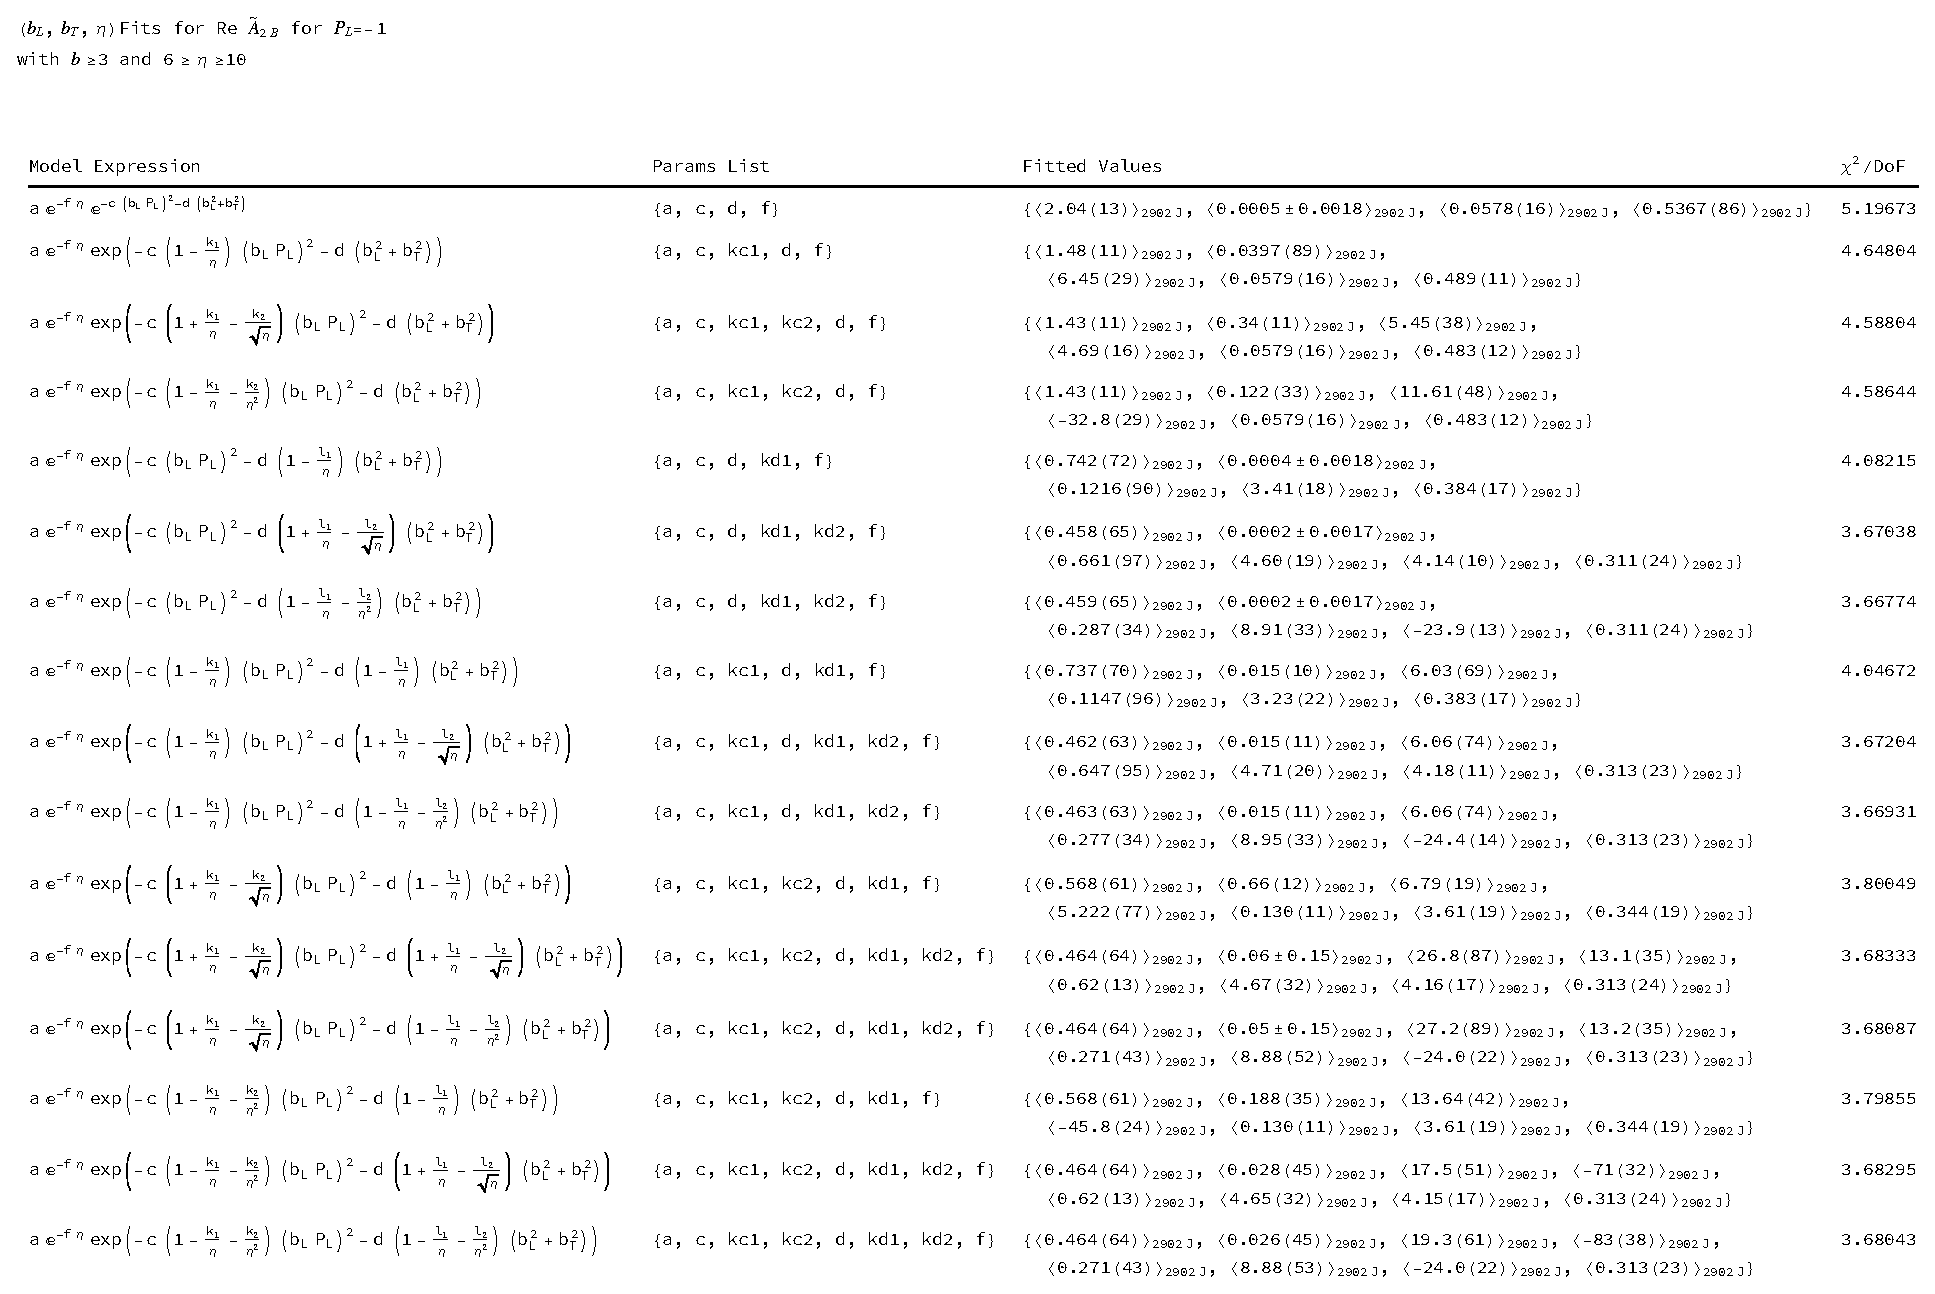
\includegraphics[width=0.8\linewidth]{plots/fit_exploration_mathematica/fit_list_gaussian_c_d_etas.eps}
    \caption{3D jackknife fits of $\mathrm{Re}\,\tilde{A}_{2B}(b_L,b_T,\eta)$ to a family of 16 Gaussian ans\"atze, all built on the common baseline $\tilde{A}_{2B} = a\, e^{-f\eta}\, \exp\!\big[-c\,(b_L P_L)^2 - d\,(b_L^2+b_T^2)\big]$, in which the coefficients $c$ and $d$ are each independently allowed to be either constant or one of three $\eta$-dependent forms, $c\to c(\eta)$ and/or $d\to d(\eta)$.}
    \label{fig:rejection_fit_list_gaussian_c_d_etas}
\end{figure}

From our physics requirements, we strictly want the fit parameter $c$ to be positive and statistically stable, because $c$ is the coefficient of $P.b$, and having a stable, positive $c$ is needed for a physical Fourier-transformed space in $x$. From Figure \ref{fig:rejection_fit_list_gaussian_c_d_etas}, most $c$ parameters are either unstable or negative, and everything still has a higher $\chi^2/\mathrm{DoF}$. On exploring power-law ans\"atze for for $\tAmp_{2B}^{\text{Re}}$ for momentum $P_L=-1$, $6\leq\eta\leq10$, and $b\geq3$, we could able to further reduce the $\chi^2/\mathrm{DoF}$ $\approx1.5$. We found that $\eta$-dependence in the fit parameter $d$ worsens the fit, while $\eta$-dependence in the fit parameter $c$ improves it. New ambiguity arises: there exist multiple $\eta$ dependencies that all give consistently the same $\chi^2/\mathrm{DoF}$. For each power-law model, the table lists the model expression, the list of fit parameters, the jackknife-averaged fitted values with statistical uncertainties, $\chi^2/\mathrm{DoF}$, AIC, and the resulting Fourier transform in $x$ space.
\begin{figure}[h!]
    \centering
    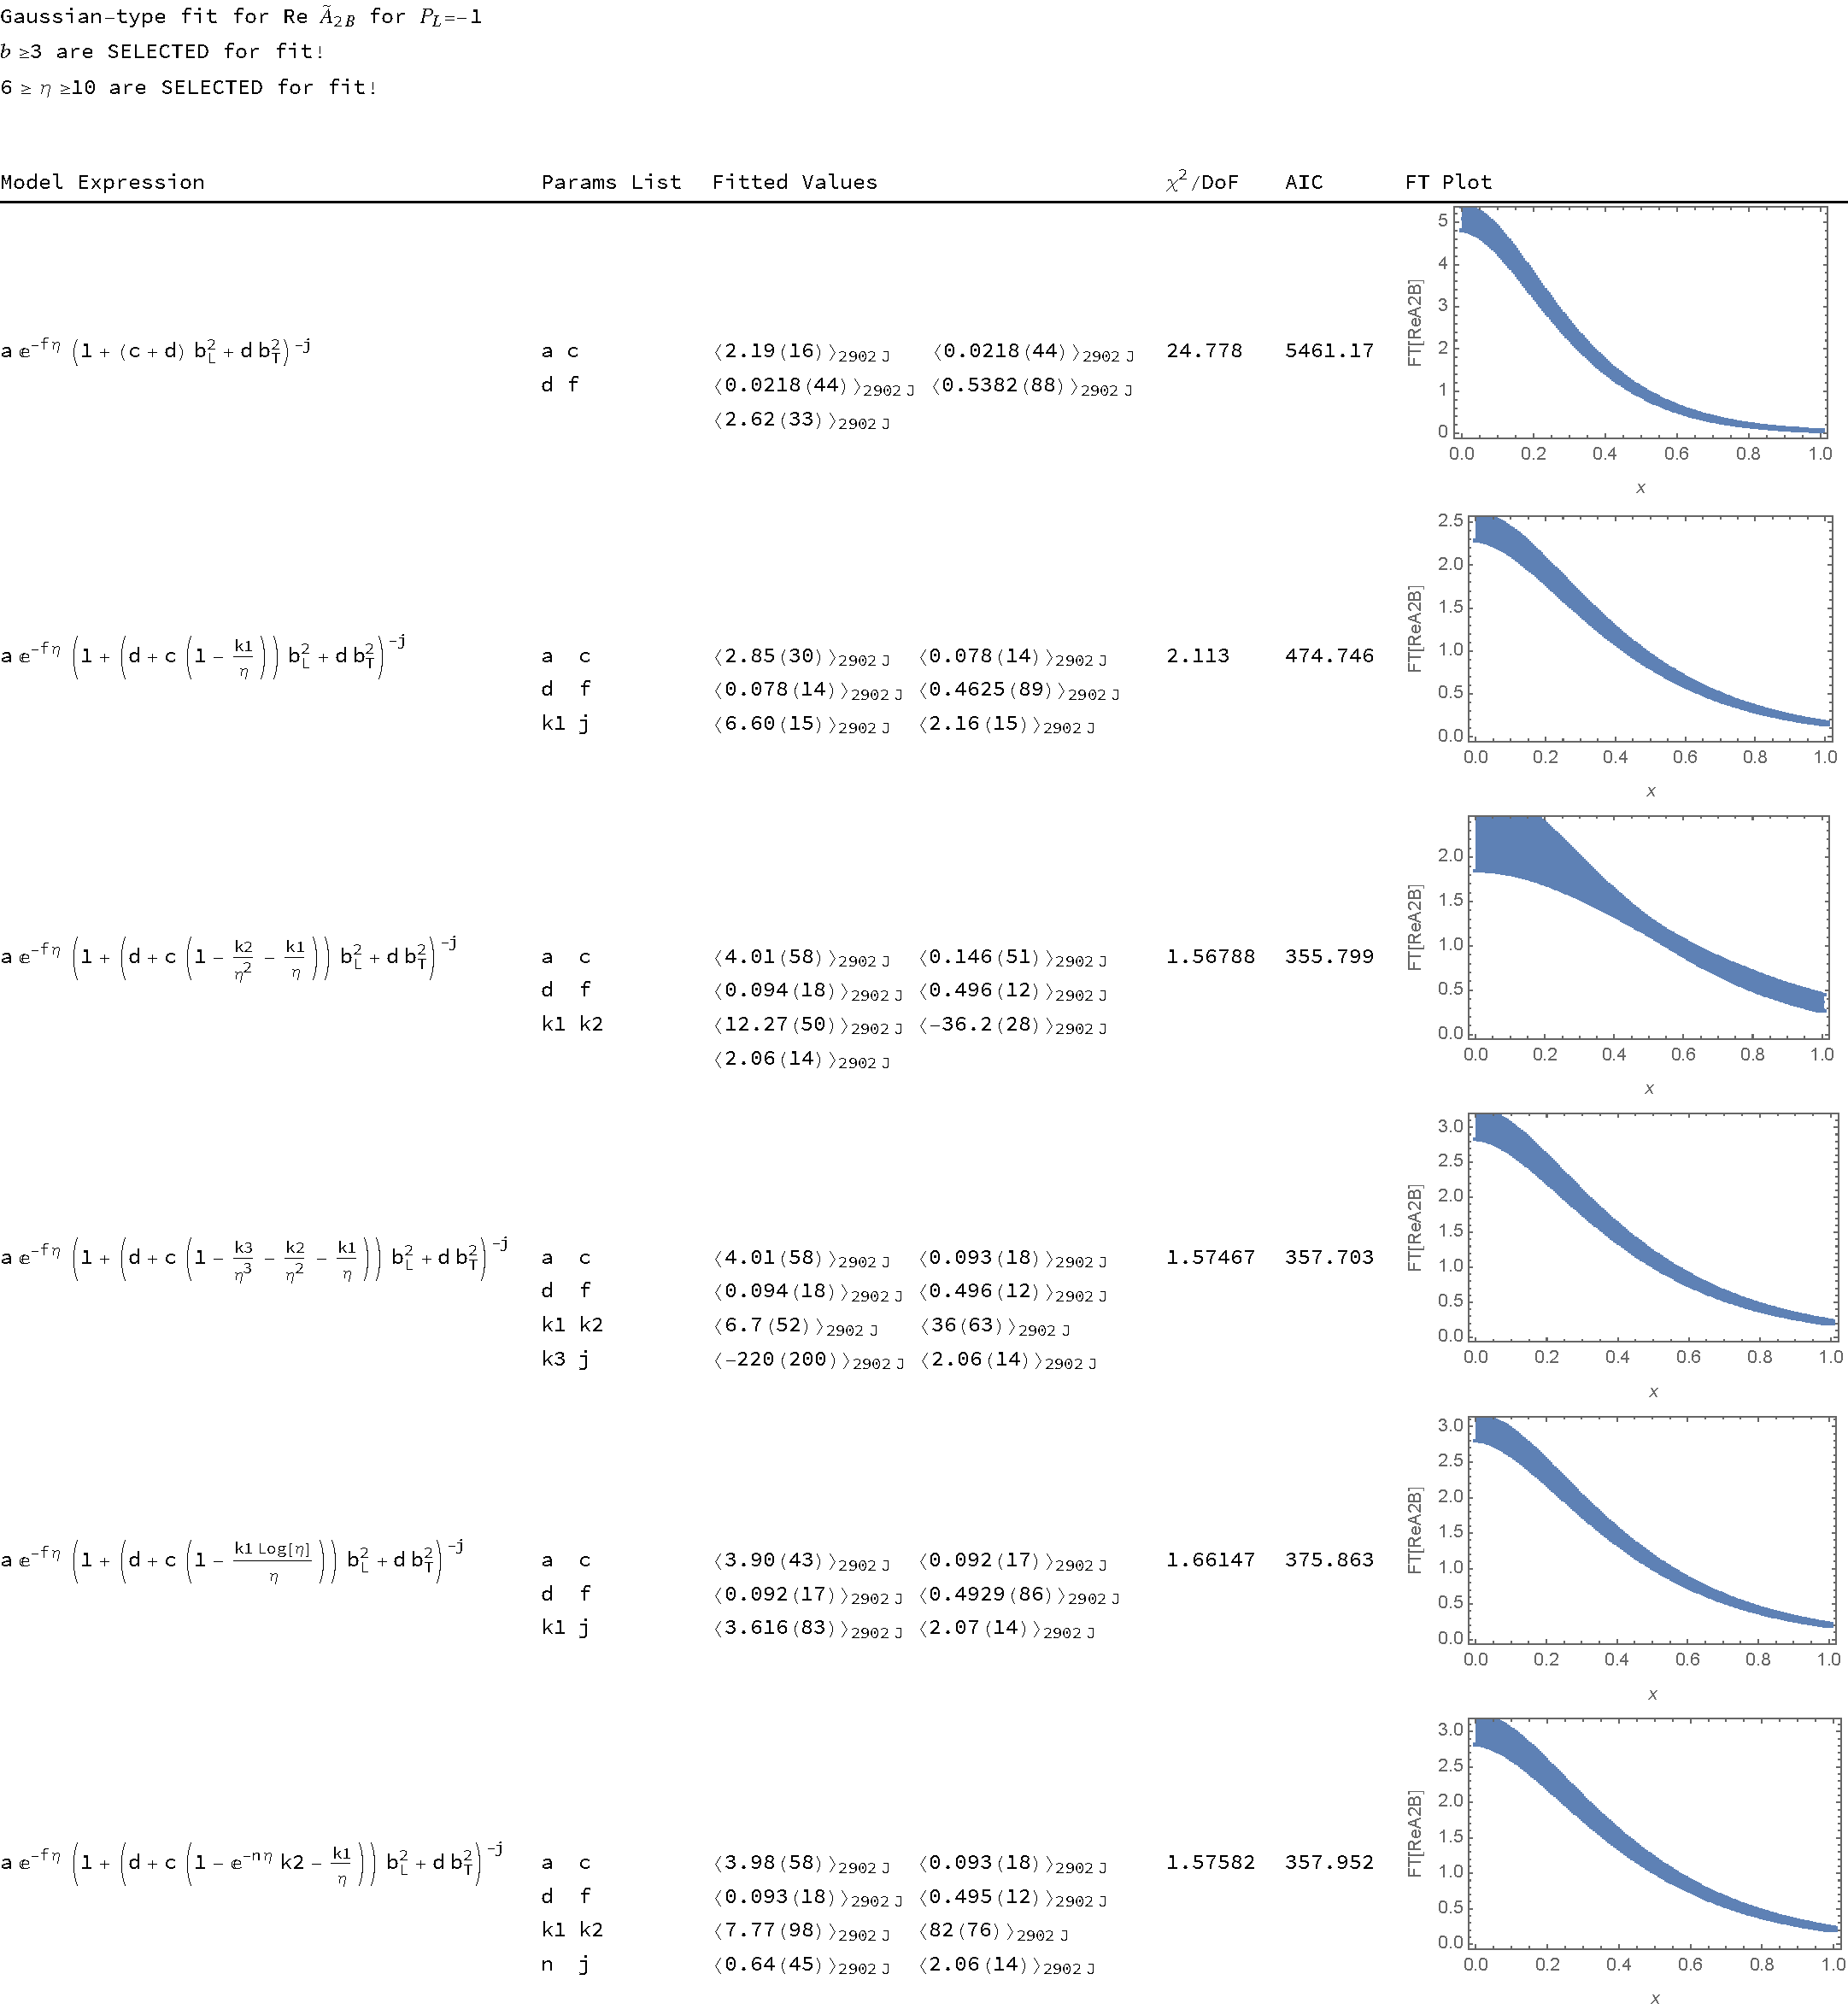
\includegraphics[width=0.8\linewidth]{PowerLaw_etaAsymptotic/A2BfitFT_eta_Asymptotic_P1.pdf}
    \caption{3D Jackknife fits of $\mathrm{Re}\,\tilde{A}_{2B}(b_L,b_T,\eta)$ to a family of power-law ans\"atze, all built on the common baseline $\tilde{A}_{2B} = a\, e^{-f\eta}\, \left(1+(c+d)b^2_L+db^2_T\right)^j$, in which the coefficient $c$ is each independently allowed to be either constant or one of $\eta$-dependent forms, $c\to c(\eta)$.}
\end{figure}
\pagebreak

For completeness, we explored more $\eta$-dependent forms $c\to c(\eta)$, which yield wider Fourier transforms in $x$ space.
\begin{figure}[h!]
    \centering
    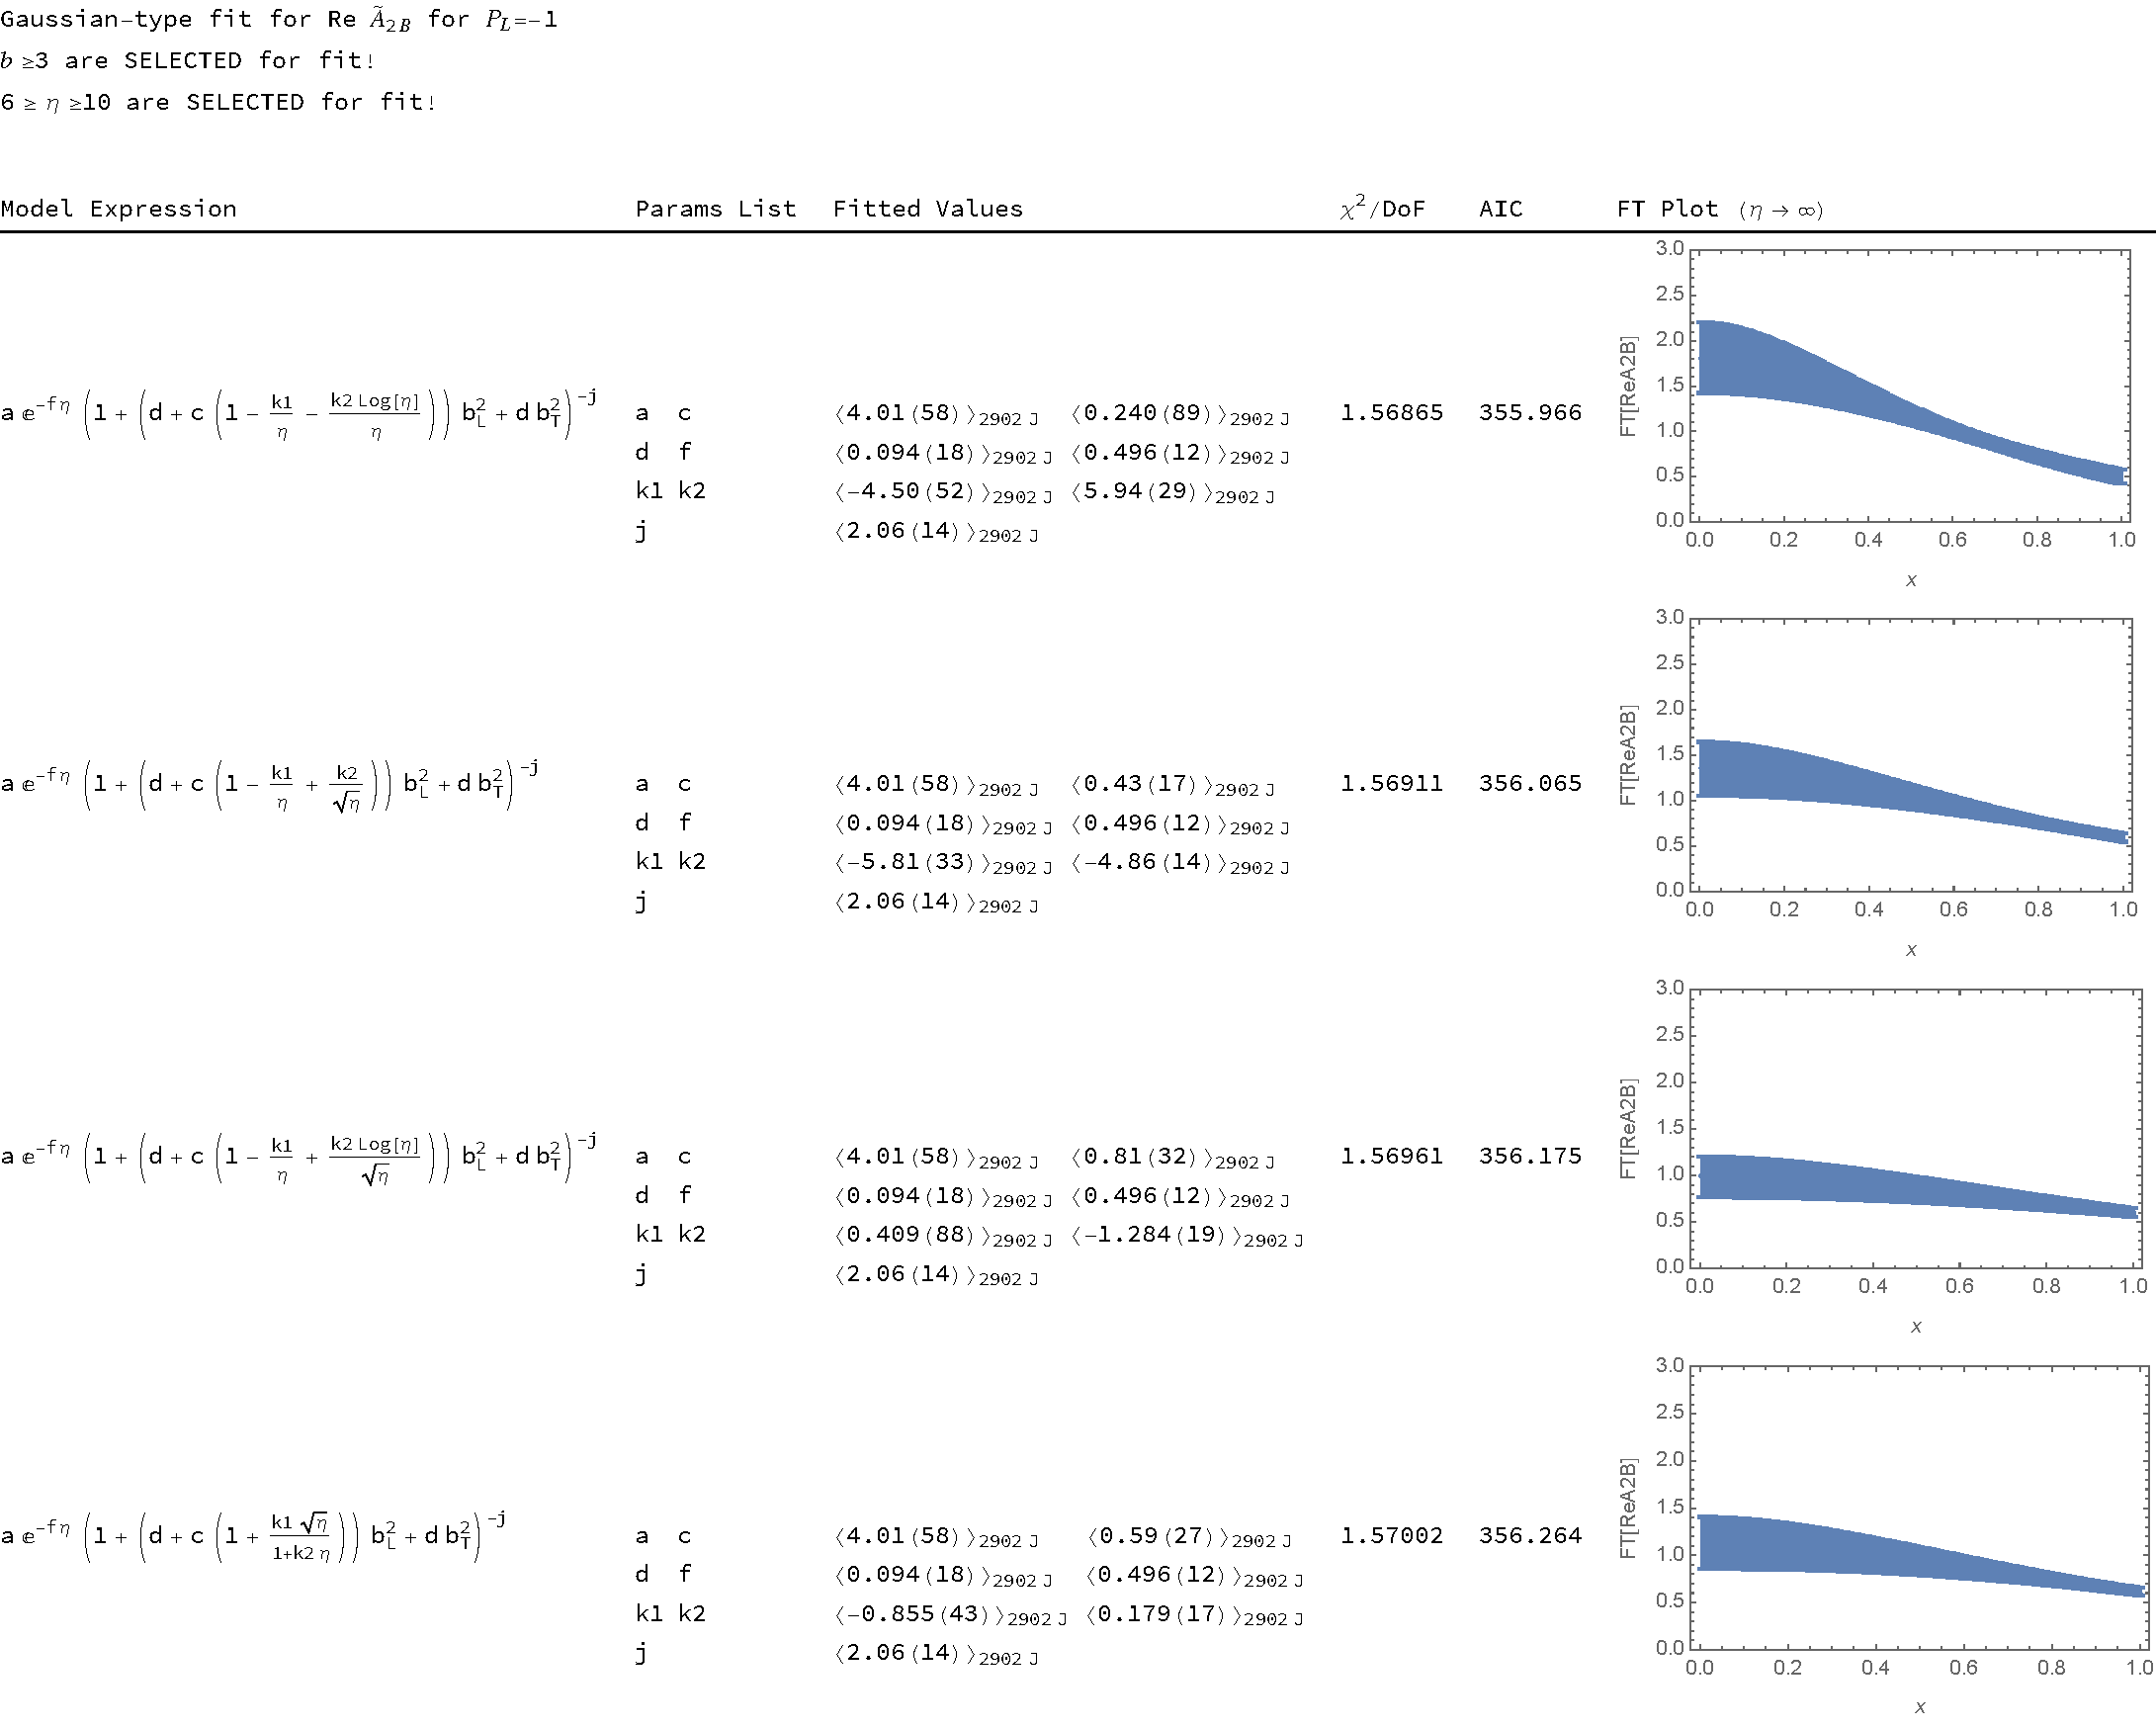
\includegraphics[width=0.8\linewidth]{PowerLaw_etaAsymptotic/A2Bfit_widerFT_eta_Asymptotic_P1.pdf}
    \caption{3D jackknife fits of $\mathrm{Re}\,\tilde{A}_{2B}(b_L,b_T,\eta)$ to a family of power-law ans\"atze, all built on the common baseline $\tilde{A}_{2B} = a\, e^{-f\eta}\, \left(1+(c+d)b^2_L+db^2_T\right)^j$, in which the coefficient $c$ is each independently allowed to $\eta$-dependent forms, $c\to c(\eta)$ which yield wider Fourier transforms in $x$ space.}
\end{figure}

All viable asymptotic functions in $\eta$ have a common power-law profile with a power $j \approx 2$ and an amplitude scale $a \approx 4$, damped by the area-law-like suppression factor $e^{-0.5\eta}$. We isolate the specific $\eta$-dependence of the width parameters $c$ and $d$ by fixing these structural parameters ($j=2$, $a=4$) and performing sequential fits at individual $\eta$ slices. The results are shown below:
\pagebreak
\begin{figure}[htbp]
    \centering
    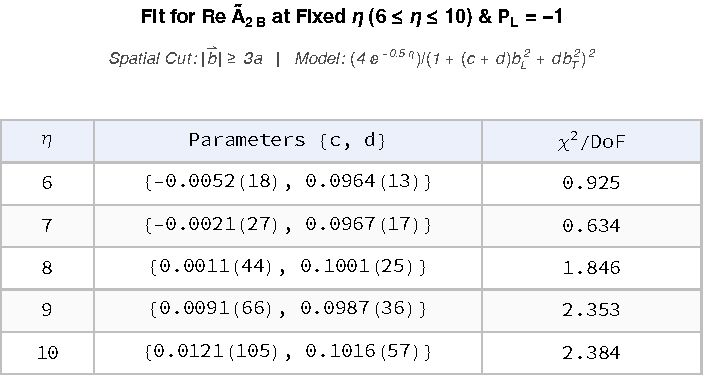
\includegraphics[width=0.6\linewidth]{Gaussian_type_fit_Real_A2B/LorentzianFixedA_P-1_b3.pdf}
    \caption{Sequential Lorentzian fits for $\tAmp^{Re}_{2B}$ at individual $\eta$ slices, holding the global power $j=2$ and amplitude $a=4$ constant.}
    \label{fig:ReA2B_fixed_eta_slices}
\end{figure}

From these fits, we extract the parameters $c$ and $d$. The fit parameter $c$ acts as a coefficient of the longitudinal separation $(P \cdot b)$, while $d$ acts as a coefficient of the invariant squared separation $b^2$. We plot the extracted values of $c$ and $d$ against our candidate asymptotic models to analyze their $\eta$-dependence:

\begin{figure}[h!]
    \centering
    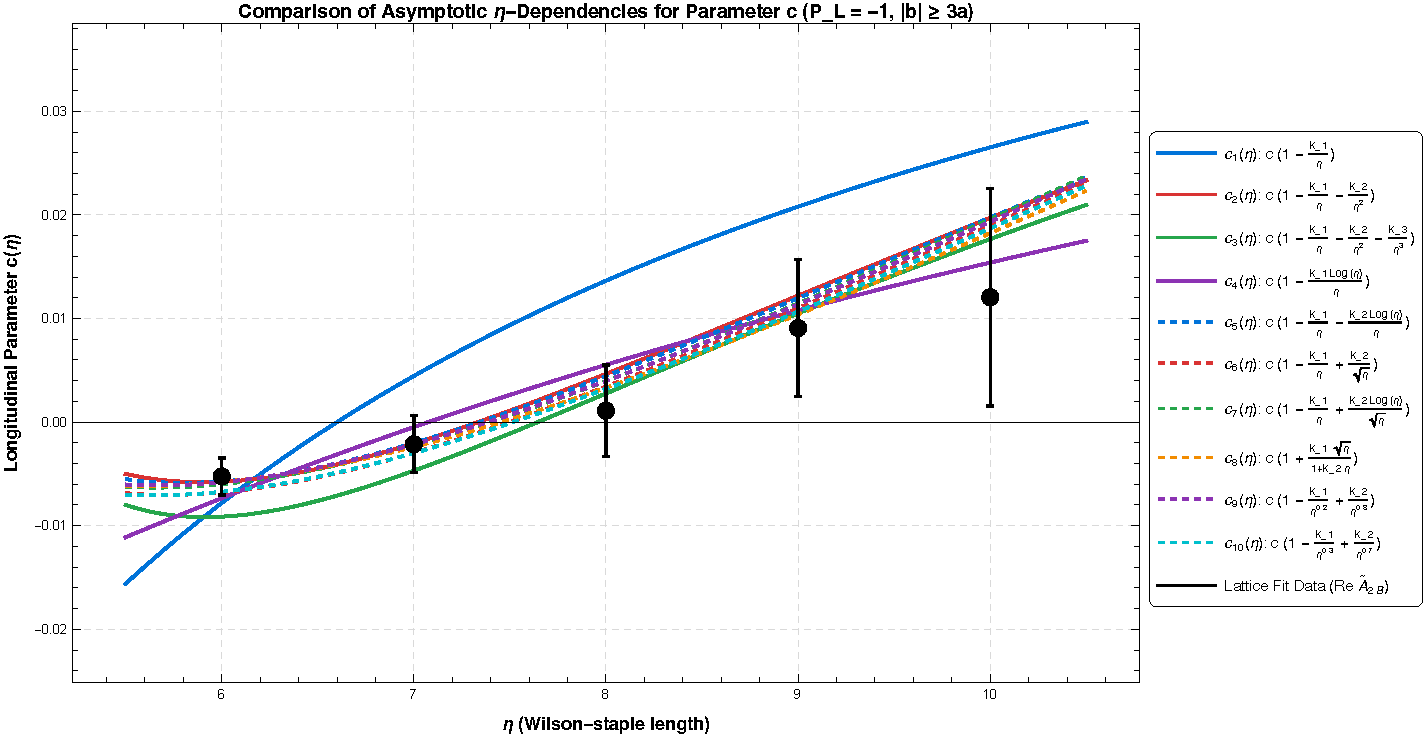
\includegraphics[width=0.5\linewidth]{PowerLaw_etaAsymptotic/A2B_c_eta_AllAsymptoticModels_P1.pdf}
    \caption{The extracted parameter $c(\eta)$ overlaid with various candidate asymptotic models, demonstrating its asymptotic approach at large $\eta$.}
\end{figure}

\begin{figure}[h!]
    \centering
    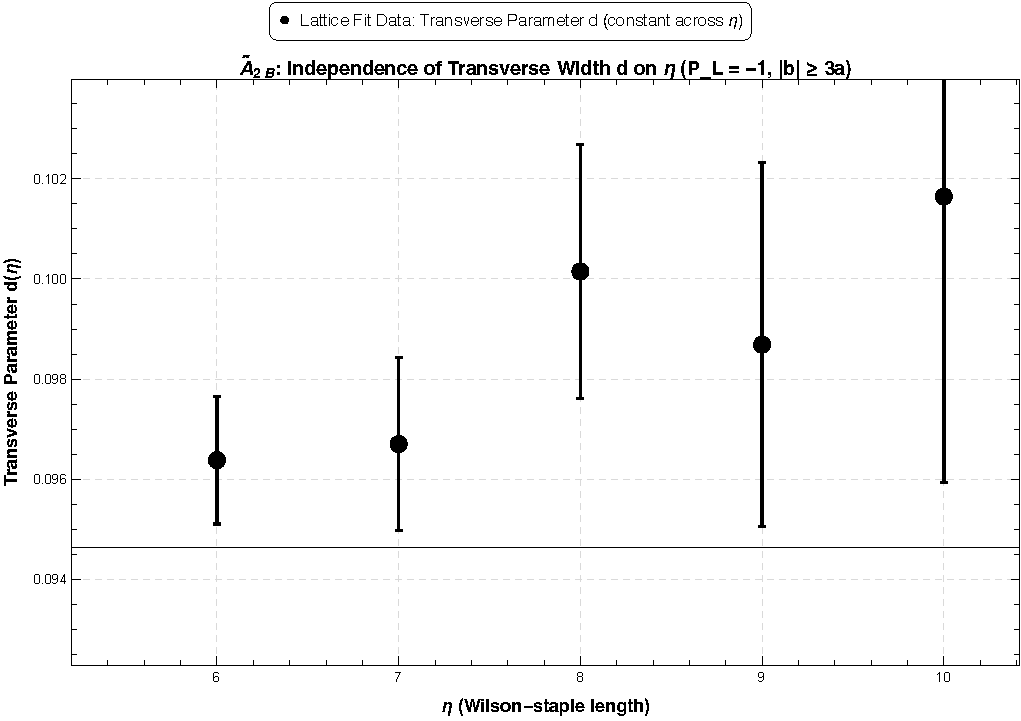
\includegraphics[width=0.4\linewidth]{PowerLaw_etaAsymptotic/A2B_d_eta_Independence_P1.pdf}
    \caption{The extracted parameter $d(\eta)$, exhibiting a clear independence from the staple extent $\eta$.}
\end{figure}


\subsection{Candidate Selection}
\label{sec:candidate_selection}

Based on the $\chi^2/\text{dof}$ minimizations and sequential fitting at individual $\eta$ slices, we determined the structural parameterizations for the invariant amplitudes: $\tAmp_{2B}^{\text{Re}}$, $\tAmp_{2B}^{\text{Im}}$, and $\tAmp_{12B}^{\text{Re}}$. We exclude $\tAmp_{12B}^{\text{Im}}$ because the lattice data is consistent with zero.

For the unpolarized real amplitude $\tAmp_{2B}^{\text{Re}}$, the transverse width parameter $d$ remains constant across all $\eta$, but the longitudinal width parameter $c(\eta)$ requires an asymptotic model. We select the model $c(\eta) = c\left(1 - \frac{k_1}{\eta} - \frac{k_2}{\eta^2}\right)$ because its Fourier transform suppresses negative-$x$ contributions, which we discuss in later sections.

For the real Sivers amplitude $\tAmp_{12B}^{\text{Re}}$, we repeated the sequential Lorentzian fitting at fixed $\eta$ slices. As shown in Fig.~\ref{fig:ReA12B_eta_independence} and Table \ref{tab:ReA12B_fixed_eta}, the longitudinal parameter $c$ and transverse parameter $d$ are independent of $\eta$. We therefore model $c$ and $d$ as constants for $\tAmp_{12B}^{\text{Re}}$.

\begin{table}[h!]
    \centering
    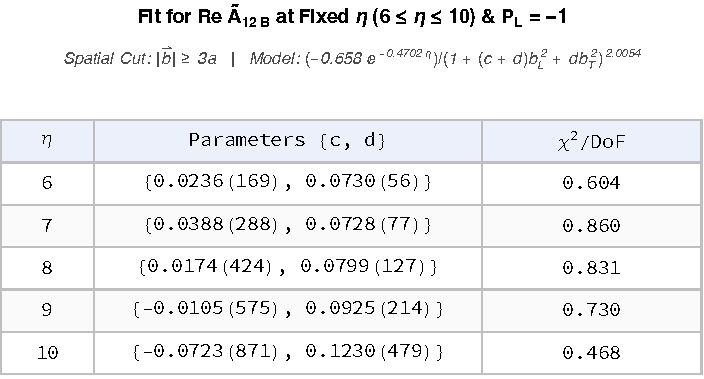
\includegraphics[width=0.55\linewidth]{Gaussian_type_fit_Real_A2B/LorentzianFixed_ReA12B_P-1_b3.pdf}
    \caption{Sequential Lorentzian fits for $\tAmp_{12B}^{\text{Re}}$ at individual $\eta$ slices showing consistent $\chi^2/\text{dof}$ and stable parameters.}
    \label{tab:ReA12B_fixed_eta}
\end{table}

\begin{figure}[h!]
    \centering
    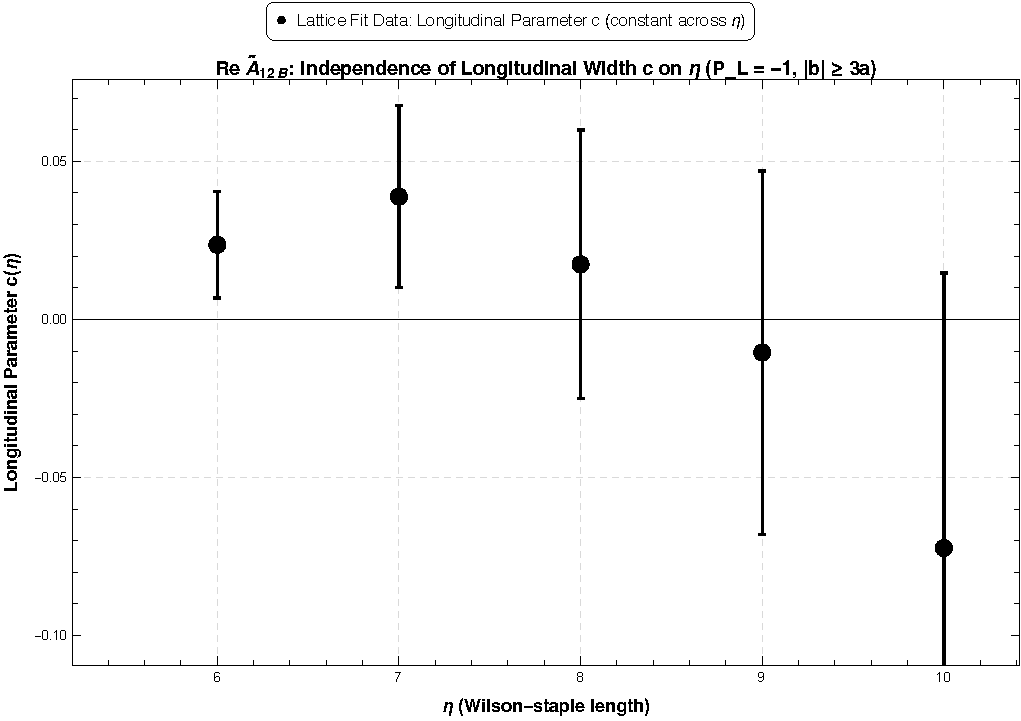
\includegraphics[width=0.49\linewidth]{PowerLaw_etaAsymptotic/ReA12B_c_eta_Independence_P1.pdf}
    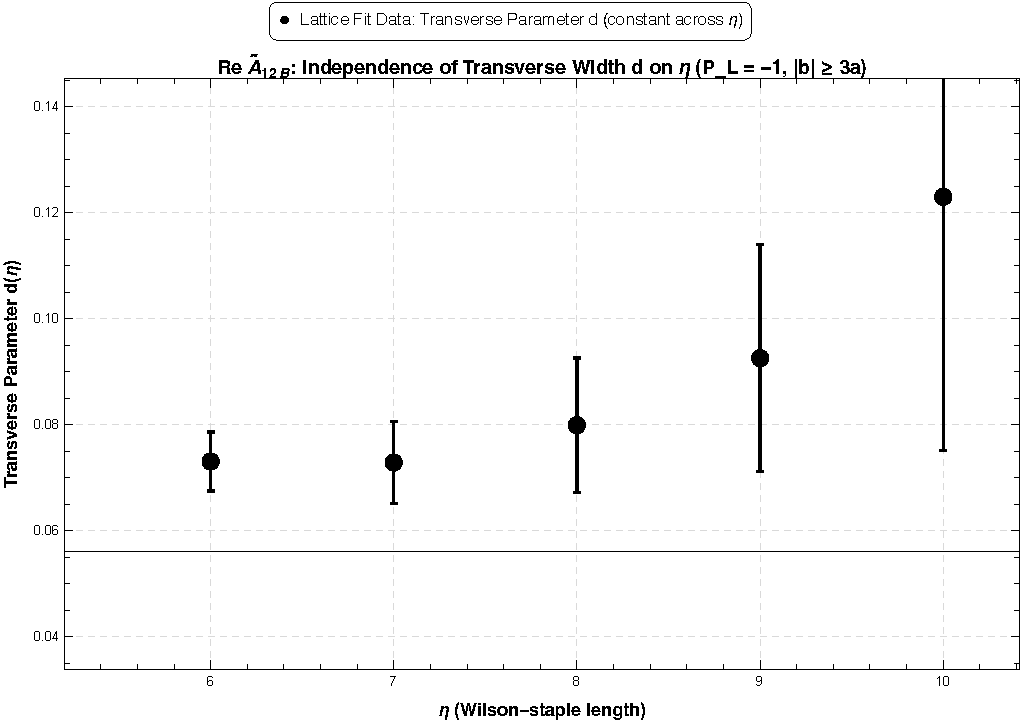
\includegraphics[width=0.49\linewidth]{PowerLaw_etaAsymptotic/ReA12B_d_eta_Independence_P1.pdf}
    \caption{Lattice extracted parameters $c$ (left) and $d$ (right) for $\tAmp_{12B}^{\text{Re}}$ as a function of $\eta$. Both parameters demonstrate clear independence from $\eta$.}
    \label{fig:ReA12B_eta_independence}
\end{figure}

For the imaginary unpolarized amplitude $\tAmp_{2B}^{\text{Im}}$, the lattice data has more statistical noise, but the sequential fitting yields a similar trend. We model $c$ and $d$ as constant in $\eta$, mirroring the structural stability of the real amplitudes. The resulting fits are shown in Fig.~\ref{fig:ImA2B_eta_independence} and Table \ref{tab:ImA2B_fixed_eta}.

\begin{table}[h!]
    \centering
    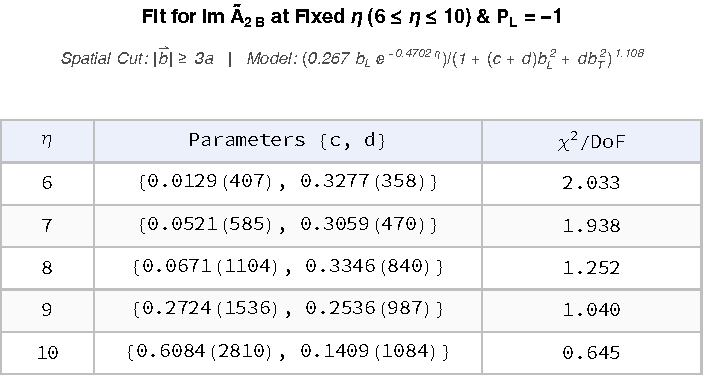
\includegraphics[width=0.55\linewidth]{Gaussian_type_fit_Real_A2B/LorentzianFixed_ImA2B_P-1_b3.pdf}
    \caption{Sequential Lorentzian fits for $\tAmp_{2B}^{\text{Im}}$ at individual $\eta$ slices showing consistent $\chi^2/\text{dof}$.}
    \label{tab:ImA2B_fixed_eta}
\end{table}

\begin{figure}[h!]
    \centering
    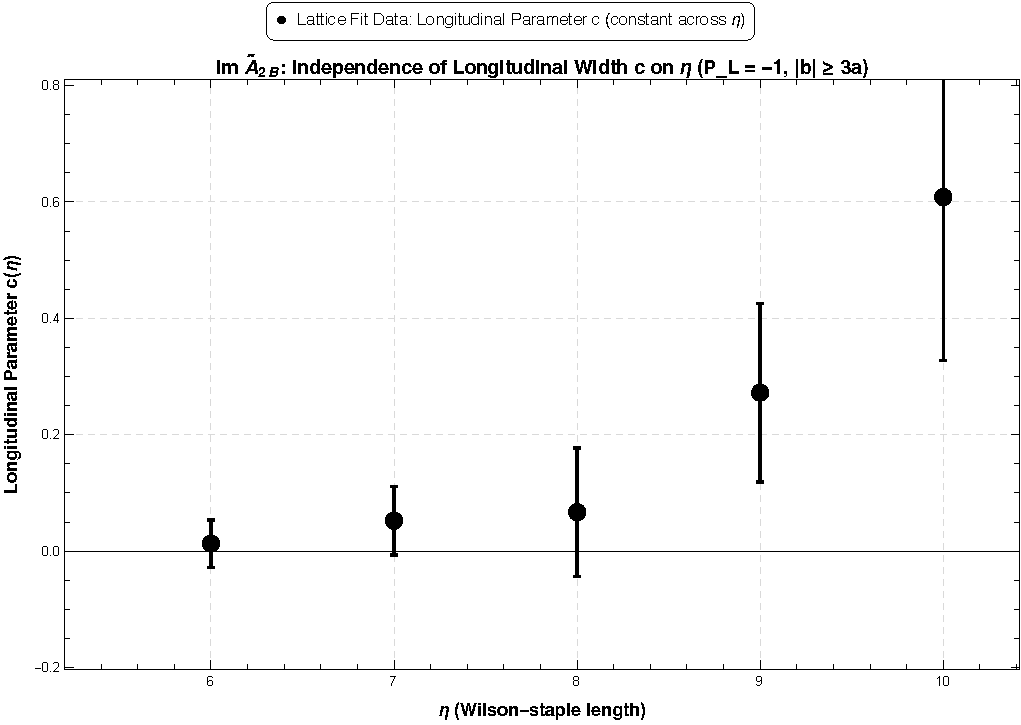
\includegraphics[width=0.49\linewidth]{PowerLaw_etaAsymptotic/ImA2B_c_eta_Independence_P1.pdf}
    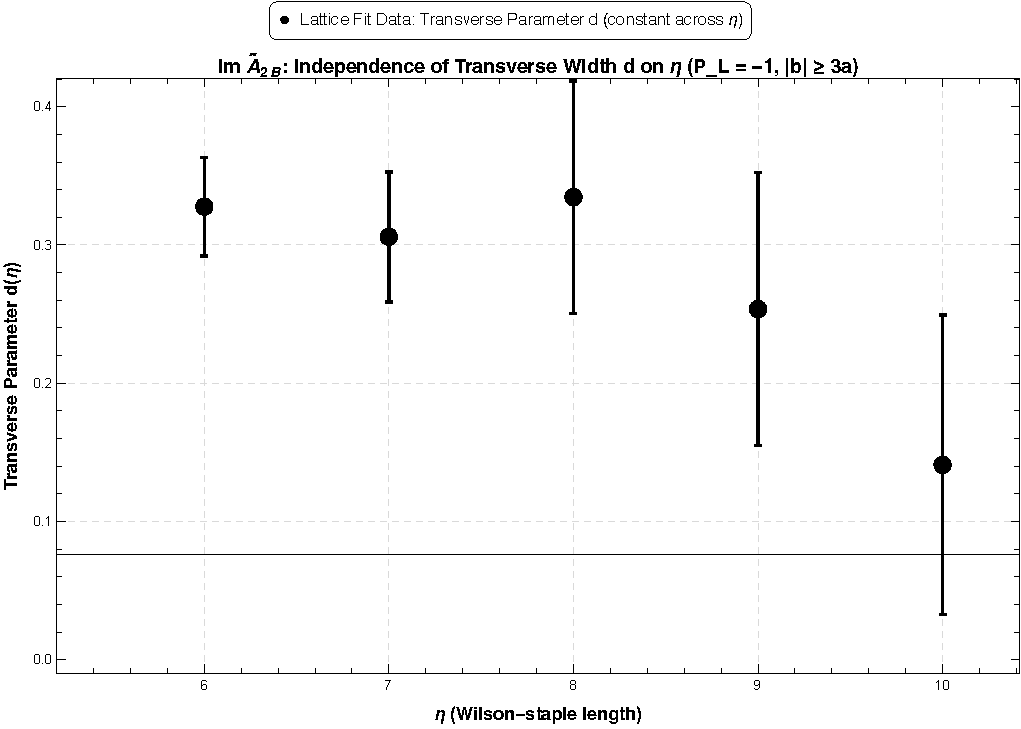
\includegraphics[width=0.49\linewidth]{PowerLaw_etaAsymptotic/ImA2B_d_eta_Independence_P1.pdf}
    \caption{Lattice extracted parameters $c$ (left) and $d$ (right) for $\tAmp_{2B}^{\text{Im}}$ as a function of $\eta$. Despite increased statistical noise, the data are highly consistent with the constant-parameter ansatz.}
    \label{fig:ImA2B_eta_independence}
\end{figure}

The analytical models in invariant $(b_L,b_T)$ space for the three amplitudes are:
\begin{align}
    \tAmp_{2B}^{\text{Re}}&=\left[\frac{a e^{-f \eta}}{\left[1 + \left(d + c\left(1 - \frac{k_1}{\eta} - \frac{k_2}{\eta^2}\right)\right) b_L^2 + d b_T^2\right]^j}\right]\label{eq:model_ReA2B}\\
    \tAmp_{12B}^{\text{Re}}&=\left[\frac{-a^{\prime} e^{-f \eta}}{\left[1 + (c^{\prime} + d^{\prime}) b_L^2 + d^{\prime} b_T^2\right]^{j^{\prime}}}\right]\label{eq:model_ReA12B}\\
    \tAmp_{2B}^{\text{Im}}&=\left[\frac{a^{\prime\prime} b_L e^{-f \eta}}{\left[1 + (c^{\prime\prime} + d^{\prime\prime}) b_L^2 + d^{\prime\prime} b_T^2\right]^{j^{\prime\prime}}}\right]\label{eq:model_ImA2B}
\end{align}


\subsection{Simultaneous Fitting Strategy}
\label{sec:simultaneous_fit_strategy}

The structural models in Eq. (\ref{eq:model_ReA2B})-(\ref{eq:model_ImA2B}) show that all three surviving amplitudes share an $\eta$-dependence damped by a common exponential decay factor, $e^{-f\eta}$. Because the Sivers shift is a ratio of transverse momentum moments, this shared exponential behavior cancels out in the physical momentum fraction $x$ calculation. 

The Sivers shift is the ratio of the first transverse momentum moment of the Sivers function to the unpolarized TMD distribution:
\begin{equation}
   \langle \vect{k}_y \rangle_{TU}(\vprp{\bvec}^2,x,\zetahat,\eta v \tcdot P) 
	\ \equiv\ \mN \frac{\tilde f_{1T}^{\perp(1)}(\vprp{\bvec}^2;\zetahat,\ldots,\eta v \tcdot P)}{\tilde f_1^{(0)}(\vprp{\bvec}^2;\zetahat,\ldots,\eta v \tcdot P)} \ .
\end{equation}

Expanding these Fourier-transformed distributions in terms of the invariant effective amplitudes $\tAmp_{12B}$ and $\tAmp_{2B}$, we rewrite the ratio as an integration over the longitudinal quark spatial separation $b \cdot P$:
\begin{equation}
    \langle \vect{k}_y \rangle_{TU} = -m_{N} \frac{\int d(b\cdot P)e^{ix(b\cdot P)} \tAmp_{12B}(\bvec^2,\bvec \tcdot P,(\bvec \tcdot P) R(\zetahat^2)/\mN^2,-1/(\mN\zetahat)^2,\eta v \tcdot P)}{\int d(b\cdot P)e^{ix(b\cdot P)}\tAmp_{2B}(\bvec^2,\bvec \tcdot P,(\bvec \tcdot P) R(\zetahat^2)/\mN^2,-1/(\mN\zetahat)^2,\eta v \tcdot P)} \ .
\end{equation}

We then decompose the complex effective amplitudes into their real (T-even) and imaginary (T-odd) components. The imaginary Sivers amplitude is statistically consistent with zero, so we remove $\tAmp_{12B}^{\text{Im}}$ from the numerator:
\begin{equation}
    \langle \vect{k}_y \rangle_{TU} = -m_{N} \frac{\int d(b\cdot P)e^{ix(b\cdot P)} \left[\tAmp_{12B}^{\text{Re}}(\cdots)+i\cancelto{0}{\tAmp_{12B}^{\text{Im}}(\cdots)}\right]}{\int d(b\cdot P)e^{ix(b\cdot P)}\left[\tAmp_{2B}^{\text{Re}}(\cdots)+i\tAmp_{2B}^{\text{Im}}(\cdots)\right]} \ .
\end{equation}

We use Euler's formula to expand the Fourier kernel $e^{ix(b\cdot P)}$ into cosine and sine components. Because the integration domain is symmetric, any integrand that is odd in $b \cdot P$ integrates to zero. Retaining only the non-vanishing even-parity combinations yields:
\begin{equation}
    \langle \vect{k}_y \rangle_{TU} = -m_{N} \frac{\int d(b\cdot P) \cos{\left(x(b\cdot P)\right)}\tAmp_{12B}^{\text{Re}}(\cdots)}{\int d(b\cdot P)\left[\cos{\left(x(b\cdot P)\right)}\tAmp_{2B}^{\text{Re}}(\cdots)-\sin{\left(x(b\cdot P)\right)}\tAmp_{2B}^{\text{Im}}(\cdots)\right]} \ .
\end{equation}
Substituting the analytical models from Eq. (\ref{eq:model_ReA2B})-(\ref{eq:model_ImA2B}) shows the shared asymptotic parameter $e^{-f \eta}$. Because the $e^{-f\eta}$ term is independent of the integration variable $b \cdot P$, it factors out of both the numerator and denominator integrals, canceling the shared exponential decay parameter. Applying the Lorentz-invariant projection $b_L = \frac{P \cdot b}{-P_L}$ and $b_T^2=b^2-b_L^2$, we arrive at the final integrands in the invariant frame:
\begin{equation}
\begin{aligned}
    \langle \vect{k}_y \rangle_{TU} &= m_{N} \frac{\int d(b\cdot P) \cos{\left(x(b\cdot P)\right)} \frac{a^{\prime}}{D_{12B}^{\text{Re}}}}{\int d(b\cdot P)\left[\cos{\left(x(b\cdot P)\right)} \frac{a}{D_{2B}^{\text{Re}}} - \sin{\left(x(b\cdot P)\right)}\frac{a^{\prime\prime} (P \cdot b) / (-P_L)}{D_{2B}^{\text{Im}}}\right]} \ , \\
    D_{12B}^{\text{Re}} &= \left[1 + (c^{\prime}) \frac{(P \cdot b)^2}{P_L^2} + d^{\prime} b^2\right]^{j^{\prime}} \ , \\
    D_{2B}^{\text{Re}} &= \left[1 + \left(c\left(1 - \frac{k_1}{\eta} - \frac{k_2}{\eta^2}\right)\right) \frac{(P \cdot b)^2}{P_L^2} + d b^2\right]^j \ , \\
    D_{2B}^{\text{Im}} &= \left[1 + (c^{\prime\prime}) \frac{(P \cdot b)^2}{P_L^2} + d^{\prime\prime} b^2\right]^{j^{\prime\prime}} \ .
\end{aligned}
\end{equation}
To enforce this shared $\eta$-dependence across the amplitudes, we use a simultaneous global fit. Forcing the parameter $f$ to be identical across all three amplitude models ($\tAmp_{2B}^{\text{Re}}$, $\tAmp_{2B}^{\text{Im}}$, and $\tAmp_{12B}^{\text{Re}}$) ensures theoretical consistency and stabilizes the parameter extraction, reflecting the physical cancellation mechanism above.


For the unpolarized real amplitude $\tAmp_{2B}^{\text{Re}}$, the transverse width parameter $d$ remains constant across all $\eta$, but the longitudinal width parameter $c(\eta)$ requires an asymptotic model.

In selecting the final model for $c(\eta)$, statistical goodness-of-fit must be paired with physical boundary conditions on the light-cone momentum fraction $x \in [-1, 1]$:

\begin{itemize}
    \item \textbf{Quark versus Anti-quark Domains}: In light-cone field theory, positive momentum fractions ($x > 0$) correspond to quark distributions $q(x) = f_1(x)$, while negative momentum fractions ($x < 0$) govern anti-quark distributions through $\bar{q}(x) = -f_1(-x)$.
    \item \textbf{Anti-quark Suppression at Large $|x|$}: In physical nucleons, sea anti-quark densities are concentrated strictly at low momentum fractions ($|x| \lesssim 0.1$). As $|x|$ increases, the anti-quark distribution falls rapidly to zero. At moderate-to-large values ($x < -0.2$ or $x < -0.3$), the anti-quark density is negligible.
    \item \textbf{Fourier Artifact Suppression}: Candidate models that approach the asymptote too slowly or fail to capture the curvature in $\eta$ (such as Candidates 2 and 5) produce unphysical oscillatory behavior or non-vanishing tails in the negative-$x$ region ($x < -0.2$) upon Fourier transformation. Candidate 1 cleanly suppresses anti-quark contributions in this regime while maintaining an optimal balance of minimal $\chi^2/\text{dof}$ and AIC score.
\end{itemize}

\subsubsection{Simultaneous Fit with Full Covariance Matrix}

Because we extract the amplitudes from the same gauge field configurations and evaluate them across nearby spatial coordinates $(b_L, b_T)$, their statistical fluctuations are highly correlated. A simple uncorrelated $\chi^2$ minimization improperly weights these data points, deflating uncertainties and biasing the central values.

To resolve this, we perform a correlated $\chi^2$ minimization utilizing the full covariance matrix. This accounts for the cross-correlations inherent in the lattice data, both across different quark spatial separations and across the real and imaginary amplitude components. 

We estimate these correlations using Jackknife resampling. Let $y_i^{(k)}$ represent the lattice evaluation of the $i$-th data point (spanning all spatial coordinates across $\tAmp_{2B}^{\text{Re}}$, $\tAmp_{2B}^{\text{Im}}$, and $\tAmp_{12B}^{\text{Re}}$) in the $k$-th Jackknife bin. The full Jackknife covariance matrix $C_{ij}$ is defined as \cite{Boram2011Covariance}:
\begin{equation}
    C_{ij} = \frac{N-1}{N} \sum_{k=1}^{N} \left( y_i^{(k)} - \bar{y}_i \right) \left( y_j^{(k)} - \bar{y}_j \right) \ ,
\end{equation}
where $N$ is the total number of Jackknife samples and $\bar{y}_i = \frac{1}{N}\sum_k y_i^{(k)}$ is the sample mean. 

The global simultaneous fit minimizes the correlated $\chi^2$ objective function with respect to the model parameters $\mathbf{p}$:
\begin{equation}
    \chi^2(\mathbf{p}) = \sum_{i,j} \left( \bar{y}_i - F_i(\mathbf{p}) \right) C_{ij}^{-1} \left( \bar{y}_j - F_j(\mathbf{p}) \right) \ ,
\end{equation}
where $F_i(\mathbf{p})$ represents the analytical models evaluated at the corresponding kinematics. 

We utilize the \texttt{lsqfit} \cite{Lepage:2001ym} non-linear least squares fitting package and the \texttt{gvar} library for Gaussian error propagation. We construct the full Jackknife covariance matrix that captures the cross-correlations between $\tAmp_{2B}^{\text{Re}}$, $\tAmp_{2B}^{\text{Im}}$, and $\tAmp_{12B}^{\text{Re}}$. The \texttt{gvar} framework binds the combined lattice data array to the inverse covariance matrix.

\subsection{Rejection of Separable Longitudinal and Transverse Factorization}
\label{sec:rejection_exponential_longitudinal}
To test this separability hypothesis discussed in Section \ref{Test-for-Factorization}, we constructed candidate models that multiply an independent longitudinal profile by various transverse $b^2$ profiles, including combinations of Gaussian, Lorentzian power-law, and exponential-decay forms. We evaluated each model with full Jackknife fits.

The fit results are summarized in Fig.~\ref{fig:rejection_exponential_longitudinal}. When exponential decay in $(P\cdot b)$ is paired with a Gaussian transverse profile, the fit is poor ($\chi^2/\text{dof} \approx 4.98$). Even for the other models, the $\chi^2/\text{dof} \approx 2$, and the coefficient $c$ governing the $(P\cdot b)$ evaluates to a negative value and is also consistent with zero within Jackknife uncertainties; this is unstable and divergent when performing a Fourier transform. 

\begin{figure}[htbp]
    \centering
    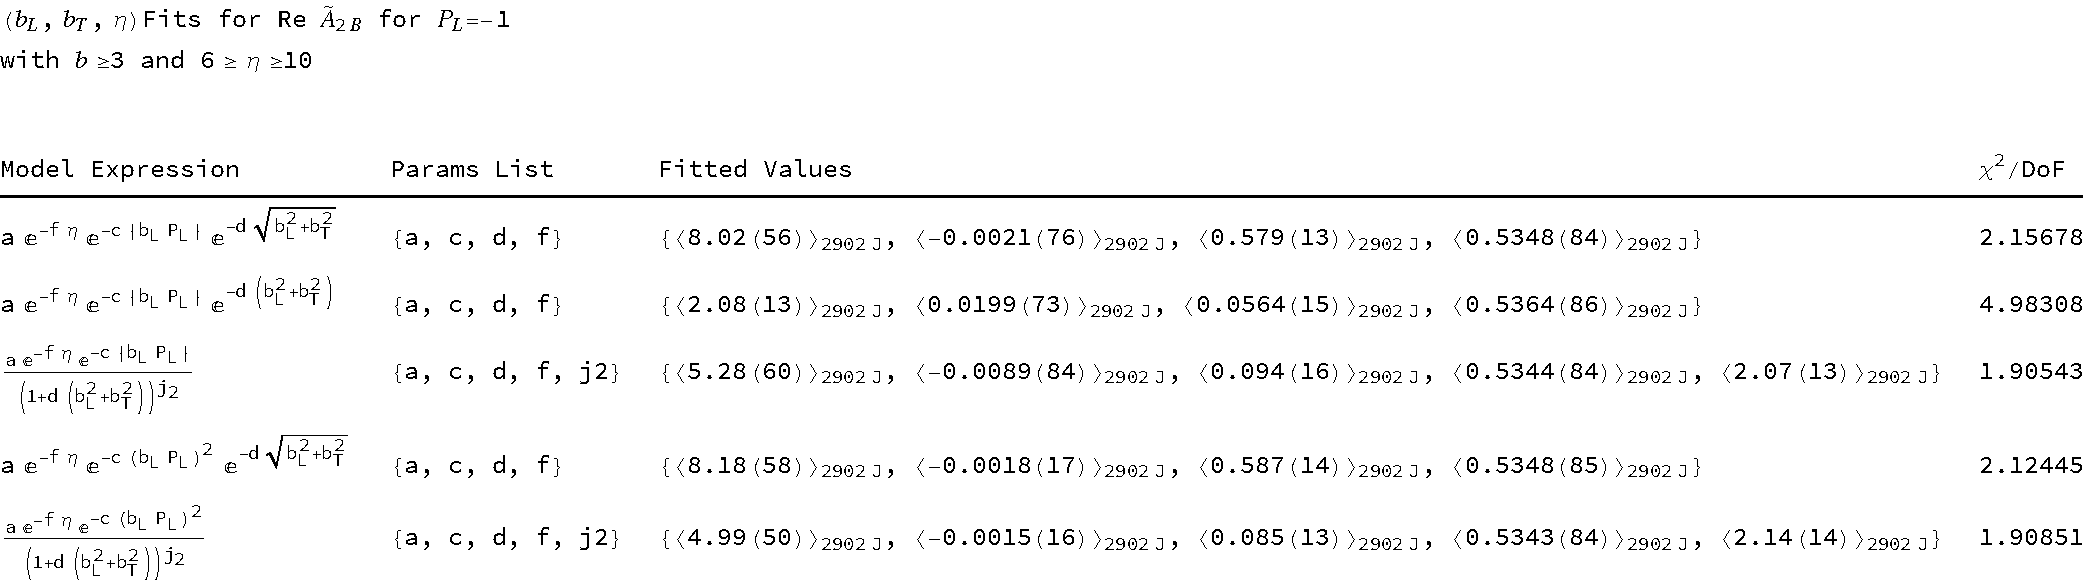
\includegraphics[width=1\linewidth]{plots/Rejection-of-Separable-Exponential-Longitudinal-Decay.pdf}
    \caption{Fit results testing the validity of the separability hypothesis: an exponential decay in $(P\cdot b)$ is paired with a Gaussian transverse profile; the fit is poor ($\chi^2/\text{dof} \approx 4.98$). In models that achieve a lower $\chi^2/\text{dof}$, the coefficient $c$ consistently fits to zero within uncertainties and is negative in each Jackknife set, demonstrating that the data rejects the separability hypothesis.}
    \label{fig:rejection_exponential_longitudinal}
\end{figure}

We also explored the separability hypothesis with $\eta$-dependent $c$, as $c(\eta)$, which governs $(P\cdot b)$; in the asymptotic limit, this forces $c$ to be positive. By introducing the asymptotic $c(\eta)$, we lowered the $\chi^2/\text{dof}$ to $ \approx 1.35$, and in the asymptotic limit $c$ is positive. From the fitting routine, we find that the lattice data prefer a power-law in $(P \cdot b)$ rather than an exponential decay in $|(P \cdot b)|$.
\begin{figure}[htbp]
    \centering
    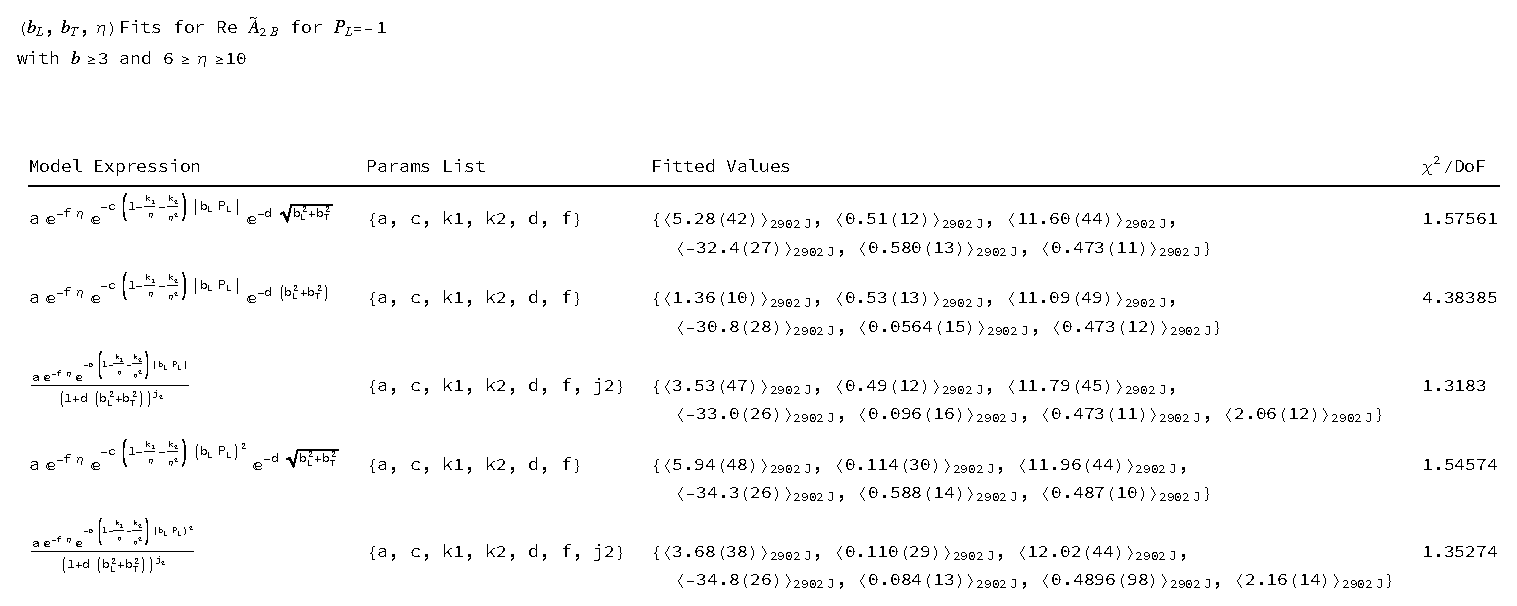
\includegraphics[width=1\linewidth]{plots/Rejection-of-Separable-Exponential-Longitudinal-Decay-ceta.eps}
    \caption{Fit results testing the validity of the separability hypothesis with $\eta$-dependent $c$, as $c(\eta)$. In models that achieve a lower $\chi^2/\text{dof}$, the coefficient $c$ is now positive}
    \label{fig:rejection_exponential_longitudinal}
\end{figure}


We systematically investigated four distinct factorized ansatze with lower $\chi^2/\text{dof}$ and propagated the same ansatze to all three invariant amplitudes ($\tAmp_{2B}^{\text{Re}}$, $\tAmp_{2B}^{\text{Im}}$, and $\tAmp_{12B}^{\text{Re}}$). These models combine either an exponential ($e^{-c|P\cdot b|}$) or Gaussian ($e^{-c(P\cdot b)^2}$) longitudinal profile with either an exponential ($e^{-d|b|}$) or power-law ($(1+db^2)^{-j}$) transverse envelope:
\begin{enumerate}
    \item \textbf{\texttt{ExpPb\_Expb}}:
    \begin{align}
        \tAmp_{2B}^{\text{Re}} &= a_{\text{re}} \, e^{-c_{\text{re}}|P\cdot b| - d_{\text{re}}|b|} \, e^{-f\eta} \ , \\
        \tAmp_{2B}^{\text{Im}} &= a_{\text{im}} \, (P\cdot b) \, e^{-c_{\text{im}}|P\cdot b| - d_{\text{im}}|b|} \, e^{-f\eta} \ , \\
        \tAmp_{12B}^{\text{Re}} &= -a_{\text{reA12B}} \, e^{-c_{\text{reA12B}}|P\cdot b| - d_{\text{reA12B}}|b|} \, e^{-f\eta} \ .
    \end{align}
    
    \item \textbf{\texttt{ExpPb\_PowerLawb}}:
    \begin{align}
        \tAmp_{2B}^{\text{Re}} &= \frac{a_{\text{re}} \, e^{-c_{\text{re}}|P\cdot b| - f\eta}}{\left(1 + d_{\text{re}} b^2\right)^{j_{\text{re}}}} \ , \\
        \tAmp_{2B}^{\text{Im}} &= \frac{a_{\text{im}} \, (P\cdot b) \, e^{-c_{\text{im}}|P\cdot b| - f\eta}}{\left(1 + d_{\text{im}} b^2\right)^{j_{\text{im}}}} \ , \\
        \tAmp_{12B}^{\text{Re}} &= \frac{-a_{\text{reA12B}} \, e^{-c_{\text{reA12B}}|P\cdot b| - f\eta}}{\left(1 + d_{\text{reA12B}} b^2\right)^{j_{\text{reA12B}}}} \ .
    \end{align}

    \item \textbf{\texttt{GaussianPb\_Expb}}:
    \begin{align}
        \tAmp_{2B}^{\text{Re}} &= a_{\text{re}} \, e^{-c_{\text{re}}(P\cdot b)^2 - d_{\text{re}}|b|} \, e^{-f\eta} \ , \\
        \tAmp_{2B}^{\text{Im}} &= a_{\text{im}} \, (P\cdot b) \, e^{-c_{\text{im}}(P\cdot b)^2 - d_{\text{im}}|b|} \, e^{-f\eta} \ , \\
        \tAmp_{12B}^{\text{Re}} &= -a_{\text{reA12B}} \, e^{-c_{\text{reA12B}}(P\cdot b)^2 - d_{\text{reA12B}}|b|} \, e^{-f\eta} \ .
    \end{align}

    \item \textbf{\texttt{GaussianPb\_PowerLawb}}:
    \begin{align}
        \tAmp_{2B}^{\text{Re}} &= \frac{a_{\text{re}} \, e^{-c_{\text{re}}(P\cdot b)^2 - f\eta}}{\left(1 + d_{\text{re}} b^2\right)^{j_{\text{re}}}} \ , \\
        \tAmp_{2B}^{\text{Im}} &= \frac{a_{\text{im}} \, (P\cdot b) \, e^{-c_{\text{im}}(P\cdot b)^2 - f\eta}}{\left(1 + d_{\text{im}} b^2\right)^{j_{\text{im}}}} \ , \\
        \tAmp_{12B}^{\text{Re}} &= \frac{-a_{\text{reA12B}} \, e^{-c_{\text{reA12B}}(P\cdot b)^2 - f\eta}}{\left(1 + d_{\text{reA12B}} b^2\right)^{j_{\text{reA12B}}}} \ .
    \end{align}
\end{enumerate}

Each model admits closed-form analytical Fourier transforms, which makes it straightforward to inspect the resulting $x$-space distributions. We performed global simultaneous Jackknife fits on these four ansatze using the same kinematic cuts ($|\vect{b}| \ge 3a$, $\eta \in [6, 10]$) and shared area-law factor $e^{-f\eta}$. The fit quality and extracted parameters are summarized in Table~\ref{tab:factorized_ansatze_comparison}.

\begin{table}[htbp]
\centering
\renewcommand{\arraystretch}{1.3}
\caption{Comparison of the four factorized longitudinal-transverse models across nucleon momenta $P_L$, with extracted parameters shown at $P_L = -1$. While models with power-law transverse envelopes describe $\tAmp_{2B}^{\text{Re}}$ passably, all four factorized ansatze fail on $\tAmp_{2B}^{\text{Im}}$ and $\tAmp_{12B}^{\text{Re}}$.}
\label{tab:factorized_ansatze_comparison}
\scalebox{0.7}{
\begin{tabular}{|l|c|c|c|c|c|c|c|p{4.2cm}|}
\hline
\textbf{Model Ansatz} & \multicolumn{4}{c|}{\textbf{$\chi^2/\text{dof}$ Across Momenta}} & \multicolumn{3}{c|}{\textbf{Key Fitted Parameters at $P_L = -1$}} & \textbf{Primary Failure Mode} \\
\cline{2-8}
& $P_L = -1$ & $P_L = -2$ & $P_L = -3$ & $P_L = -4$ & $c_{\text{im}}$ & $c_{\text{reA12B}}$ & $a_{\text{im}}$ & \\
\hline
\texttt{ExpPb\_Expb} & $1.406(92)$ & $0.956(75)$ & $0.622(61)$ & $0.455(53)$ & $0.0010(262)$ & $0.045(23)$ & $-0.167(16)$ & $c_{\text{im}} \to 0$; unphysical sign on $a_{\text{im}}$. \\
\hline
\texttt{ExpPb\_PowerLawb} & $1.286(89)$ & $0.938(75)$ & $0.623(61)$ & $0.447(53)$ & $0.0045(248)$ & $0.028(24)$ & $-0.167(31)$ & Fits $\tAmp_{2B}^{\text{Re}}$ well, but $c_{\text{im}}$ and $c_{\text{reA12B}}$ vanish within error; flips sign of $a_{\text{im}}$. \\
\hline
\texttt{GaussianPb\_Expb} & $2.389(121)$ & $2.005(111)$ & $0.945(76)$ & $0.453(52)$ & $0.568(171)$ & $0.0038(69)$ & $+0.050(121)$ & Poor $\chi^2/\text{dof}$; $c_{\text{reA12B}}$ pinned near zero; Gaussian over-damping at large $x$. \\
\hline
\texttt{GaussianPb\_PowerLawb} & $2.316(120)$ & $1.981(111)$ & $0.948(76)$ & $0.448(52)$ & $0.602(48)$ & $0.0016(61)$ & $+0.168(92)$ & Poor global fit at low momenta; $c_{\text{reA12B}} \approx 0$; unphysical truncation of valence tails. \\
\hline
\textbf{Coupled Lorentzian} & \multicolumn{4}{c|}{\textbf{$1.85(10)$ (Correlated Covariance Fit)}} & $\mathbf{0.2253(69)}$ & $\mathbf{0.0773(46)}$ & $\mathbf{+0.267(13)}$ & \textbf{All parameters stable, positive, and well-constrained across all amplitudes.} \\
\hline
\end{tabular}
}
\end{table}

The numerical results highlight several critical failure mechanisms inherent to factorized models. In \texttt{ExpPb\_PowerLawb}, the real unpolarized amplitude fits with $\chi^2/\text{dof} \approx 1.286$. Because $\tAmp_{2B}^{\text{Re}}$ dominates the statistical weight, an uncritical fit can give the false impression of an adequate model. However, the same parameterization fails for the imaginary amplitude $\tAmp_{2B}^{\text{Im}}$: the longitudinal decay width $c_{\text{im}} = 0.0045 \pm 0.0248$ evaluates to zero within errors. This means the model loses its longitudinal decay profile, producing an essentially flat distribution in $P\cdot b$. Furthermore, the overall amplitude flips to an unphysical negative sign ($a_{\text{im}} = -0.167$).

For the real Sivers amplitude $\tAmp_{12B}^{\text{Re}}$, the longitudinal parameter $c_{\text{reA12B}}$ is similarly suppressed across all factorized models ($0.028 \pm 0.024$ for \texttt{ExpPb\_PowerLawb} and $0.0016 \pm 0.0061$ for \texttt{GaussianPb\_PowerLawb}). The factorized models cannot capture the distinct longitudinal curvature of the spin-dependent correlator without forcing the decay parameter to its lower boundary. Factoring out an exponential $|P\cdot b|$ dependence introduces a discontinuous first derivative (a cusp) at $P\cdot b = 0$. For an odd-parity amplitude like $\tAmp_{2B}^{\text{Im}}$, which must vanish linearly through the origin ($\tAmp_{2B}^{\text{Im}} \propto b_L$), the non-analytic factor $e^{-c|P\cdot b|}$ conflicts with the smooth behavior of the Euclidean correlation function. The fit responds by driving $c_{\text{im}} \to 0$ to minimize the cusp penalty.

In the Lorentz-invariant variable space $(P\cdot b, b^2)$, the longitudinal separation $b_L = (P\cdot b)/(-P_L)$ and transverse separation $b_T = \sqrt{b^2 - b_L^2}$ are geometrically coupled. Factorized models force an artificial independence between $P\cdot b$ and $b^2$. In contrast, coupling $(P\cdot b)^2$ and $b^2$ within a single denominator,
    \begin{equation}
        D = \left[ 1 + c(\eta) \frac{(P\cdot b)^2}{P_L^2} + d\,b^2 \right]^j \ ,
    \end{equation}
preserves smooth analyticity at $P\cdot b = 0$, satisfies power-law integrability, and yields stable, positive parameters across all three amplitudes (e.g., $c_{\text{im}} = 0.2253(69)$, $c_{\text{reA12B}} = 0.0773(46)$, $a_{\text{im}} = +0.267(13)$). We therefore exclude factorized ansatze and adopt the coupled Lorentzian denominator for the global analysis.

The following subsections present the results of these simultaneous covariance matrix fits evaluated at discrete lattice momenta.

\renewcommand{\PLval}{-1}
\subsubsection{\texorpdfstring{Simultaneous Fit Results for $\vect{P}\cdot a\hat{L}/(2\pi)=\{\PLval,0,0\}$}{TEXT}}

The extracted parameters from the simultaneous fit for the lowest simulated nucleon momentum, $P_1 = -1$ ($\hat{\zeta} \approx 0.091$), are summarized below. Enforcing the shared asymptotic decay parameter $f$ across all three effective amplitudes ($\tAmp_{2B}^{\text{Re}}$, $\tAmp_{2B}^{\text{Im}}$, and $\tAmp_{12B}^{\text{Re}}$) stabilizes the extraction of the spatial profiles and preserves the cancellation required for the Sivers shift ratio.

\input{SimultaneousFitsCov/Fit_Table_PL\PLval_bmin3}

Figures \ref{fig:A2B_amplitudes_fit_P1} and \ref{fig:combined_fit_P1} show the results of the correlated minimization. The parameterization, shown as continuous surfaces with shaded error bands, matches the discrete lattice data across the Cartesian $(b_L/a, b_T/a)$ grid and the Lorentz-invariant $(P \cdot b, b^2)$ variable space. Excluding the short-distance data ($|\vect{b}| < 3a$) ensures the fit captures long-range dynamics without ultraviolet lattice artifacts skewing the results.

\begin{figure}[htbp]
    \centering
    \begin{tabular}{ccc}
        % Column Headers
        \textbf{$\widetilde{A}^{Re}_{2B}$} & \textbf{$\widetilde{A}^{Im}_{2B}$} & \textbf{$\widetilde{A}^{Re}_{12B}$} \\[2ex]
        \includegraphics[width=0.3\linewidth]{plots/Amps_Fit/ReA12B_Pb_bsq_PL\PLval_WithFit_3D.pdf} &
        \includegraphics[width=0.3\linewidth]{plots/Amps_Fit/ImA2B_PL\PLval_WithFit_3D.pdf} &
        \includegraphics[width=0.3\linewidth]{plots/Amps_Fit/ReA12B_PL\PLval_WithFit_3D.pdf}\\[2ex]
        \includegraphics[width=0.3\linewidth]{plots/Amps_Fit/ReA2B_Pb_bsq_PL\PLval_WithFit_3D.pdf} &
        \includegraphics[width=0.3\linewidth]{plots/Amps_Fit/ImA2B_Pb_bsq_PL\PLval_WithFit_3D.pdf} &
        \includegraphics[width=0.3\linewidth]{plots/Amps_Fit/ReA12B_Pb_bsq_PL\PLval_WithFit_3D.pdf} \\
    \end{tabular}
    \caption{Fit for $\widetilde{A}^{Re}_{2B}$, $\widetilde{A}^{Im}_{2B}$ \& $\widetilde{A}^{Re}_{12B}$ amplitudes for $\vect{P}\cdot a\hat{L}/(2\pi)=\{\PLval,0,0\}$. The top row displays the $(b_{L}/a,b_{T}/a,\eta|\vect{v}|/a)-$space, while the bottom row displays the $((\vect{P}\cdot \vect{b})\cdot\hat{L}/(2\pi),b^{2}/a^2,\eta|\vect{v}|/a)-$space with the global simultaneous fit overlaid.}
    \label{fig:A2B_amplitudes_fit_P1}
\end{figure}

\begin{figure}[htbp]
    \centering
    \begin{tabular}{c}
        \includegraphics[width=0.9\linewidth]{plots/Amps_Fit/Combined_eta8_PL\PLval_WithFit_2D.pdf} \\
        \includegraphics[width=0.9\linewidth]{plots/Amps_Fit/Combined_Pb_bsq_eta8_PL\PLval_WithFit_2D.pdf} \\
    \end{tabular}
    \caption{Fit for $\widetilde{A}^{Re}_{2B}$, $\widetilde{A}^{Im}_{2B}$ \& $\widetilde{A}^{Re}_{12B}$ amplitudes for $\vect{P}\cdot a\hat{L}/(2\pi)=\{\PLval,0,0\}$ at a fixed staple extent $\eta|\vect{v}|/a=8$. The top two rows display the $(b_{L}/a,b_{T}/a)-$space, while the bottom two rows display the $((\vect{P}\cdot \vect{b})\cdot\hat{L}/(2\pi),b^{2}/a^2)-$space with the fit.}
    \label{fig:combined_fit_P1}
\end{figure}

\pagebreak

Using the continuous parametrization of the effective amplitudes, we analytically evaluate the Fourier integrals over the invariant scalar $P \cdot b$. The results of these integrations, which yield the momentum fraction $x$-dependent unpolarized distribution and the Sivers shift, are tabulated below.

\input{SimultaneousFitsCov/Integration_Table_PL\PLval_bmin3}

The figures below show the Jackknife covariance matrix. The off-diagonal elements in the 2D correlation matrix and the 3D surface plot show cross-correlations between spatial lattice points and across amplitude components. Incorporating this covariance structure into the fitting pipeline via \texttt{lsqfit} properly weights the correlated fluctuations to determine the error bands on the final extracted Sivers shift.

\begin{figure}[htbp]
    \centering
    \includegraphics[width=0.5\linewidth]{SimultaneousFitsCov/SimulFitCovMatrix-A12B-A2B-FT-a_im-a_re-a_reA12B-c_im-c_re-c_reA12B-d_im-d_re-d_reA12B-f-j_im-j_re-j_reA12B-k1_re-k2_re__bmin3_eta610_PL\PLval.pdf}
    \caption{2D representation of the full Jackknife covariance matrix utilized in the simultaneous fit for $P_1=-1$. The prominent off-diagonal bands highlight the strong correlations across the parameter space.}
    \label{fig:cov_matrix_2d_P1}
\end{figure}

\begin{figure}[htbp]
    \centering
    \includegraphics[width=0.7\linewidth]{SimultaneousFitsCov/SimulFitCovMatrix-A12B-A2B-FT-3D_a_im-a_re-a_reA12B-c_im-c_re-c_reA12B-d_im-d_re-d_reA12B-f-j_im-j_re-j_reA12B-k1_re-k2_re__bmin3_eta610_PL\PLval.pdf}
    \caption{3D surface plot of the Jackknife covariance matrix for $P_1=-1$, visually emphasizing the magnitude of the cross-correlations between the real and imaginary amplitude components.}
    \label{fig:cov_matrix_3d_P1}
\end{figure}
\pagebreak

\pagebreak
\renewcommand{\PLval}{-2}
\subsubsection{\texorpdfstring{Simultaneous Fit Results for $\vect{P}\cdot a\hat{L}/(2\pi)=\{\PLval,0,0\}$}{TEXT}}
\input{SimultaneousFitsCov/Fit_Table_PL\PLval_bmin3}
\begin{figure}[htbp]
    \centering
    \begin{tabular}{ccc}
        % Column Headers
        \textbf{$\widetilde{A}^{Re}_{2B}$} & \textbf{$\widetilde{A}^{Im}_{2B}$} & \textbf{$\widetilde{A}^{Re}_{12B}$} \\[2ex]
        \includegraphics[width=0.3\linewidth]{plots/Amps_Fit/ReA12B_Pb_bsq_PL\PLval_WithFit_3D.pdf} &
        \includegraphics[width=0.3\linewidth]{plots/Amps_Fit/ImA2B_PL\PLval_WithFit_3D.pdf} &
        \includegraphics[width=0.3\linewidth]{plots/Amps_Fit/ReA12B_PL\PLval_WithFit_3D.pdf}\\[2ex]
        \includegraphics[width=0.3\linewidth]{plots/Amps_Fit/ReA2B_Pb_bsq_PL\PLval_WithFit_3D.pdf} &
        \includegraphics[width=0.3\linewidth]{plots/Amps_Fit/ImA2B_Pb_bsq_PL\PLval_WithFit_3D.pdf} &
        \includegraphics[width=0.3\linewidth]{plots/Amps_Fit/ReA12B_Pb_bsq_PL\PLval_WithFit_3D.pdf} \\
    \end{tabular}
    \caption{Fit for $\widetilde{A}^{Re}_{2B}$, $\widetilde{A}^{Im}_{2B}$ \& $\widetilde{A}^{Re}_{12B}$ amplitudes for $\vect{P}\cdot a\hat{L}/(2\pi)=\{\PLval,0,0\}$. The top row displays the $(b_{L}/a,b_{T}/a,\eta|\vect{v}|/a)-$space, while the bottom row displays the $((\vect{P}\cdot \vect{b})\cdot\hat{L}/(2\pi),b^{2}/a^2,\eta|\vect{v}|/a)-$space with the global simultaneous fit overlaid.}
    \label{fig:A2B_amplitudes_fit_P2}
\end{figure}

\begin{figure}[htbp]
    \centering
    \begin{tabular}{c}
        \includegraphics[width=0.9\linewidth]{plots/Amps_Fit/Combined_eta8_PL\PLval_WithFit_2D.pdf} \\
        \includegraphics[width=0.9\linewidth]{plots/Amps_Fit/Combined_Pb_bsq_eta8_PL\PLval_WithFit_2D.pdf} \\
    \end{tabular}
    \caption{Fit for $\widetilde{A}^{Re}_{2B}$, $\widetilde{A}^{Im}_{2B}$ \& $\widetilde{A}^{Re}_{12B}$ amplitudes for $\vect{P}\cdot a\hat{L}/(2\pi)=\{\PLval,0,0\}$ at a fixed staple extent $\eta|\vect{v}|/a=8$. The top two rows display the $(b_{L}/a,b_{T}/a)-$space, while the bottom two rows display the $((\vect{P}\cdot \vect{b})\cdot\hat{L}/(2\pi),b^{2}/a^2)-$space with the fit.}
    \label{fig:combined_fit_P2}
\end{figure}

\pagebreak
\input{SimultaneousFitsCov/Integration_Table_PL\PLval_bmin3}

\begin{figure}[htbp]
    \centering
    \includegraphics[width=0.5\linewidth]{SimultaneousFitsCov/SimulFitCovMatrix-A12B-A2B-FT-a_im-a_re-a_reA12B-c_im-c_re-c_reA12B-d_im-d_re-d_reA12B-f-j_im-j_re-j_reA12B-k1_re-k2_re__bmin3_eta610_PL\PLval.pdf}
    \caption{2D representation of the full Jackknife covariance matrix utilized in the simultaneous fit for $P_L=-2$.}
    \label{fig:cov_matrix_2d_P2}
\end{figure}

\begin{figure}[htbp]
    \centering
    \includegraphics[width=0.7\linewidth]{SimultaneousFitsCov/SimulFitCovMatrix-A12B-A2B-FT-3D_a_im-a_re-a_reA12B-c_im-c_re-c_reA12B-d_im-d_re-d_reA12B-f-j_im-j_re-j_reA12B-k1_re-k2_re__bmin3_eta610_PL\PLval.pdf}
    \caption{3D surface plot of the Jackknife covariance matrix for $P_L=-2$.}
    \label{fig:cov_matrix_3d_P2}
\end{figure}

\pagebreak
\renewcommand{\PLval}{-3}
\subsubsection{\texorpdfstring{Simultaneous Fit Results for $\vect{P}\cdot a\hat{L}/(2\pi)=\{\PLval,0,0\}$}{TEXT}}
\input{SimultaneousFitsCov/Fit_Table_PL\PLval_bmin3}
\begin{figure}[htbp]
    \centering
    \begin{tabular}{ccc}
        % Column Headers
        \textbf{$\widetilde{A}^{Re}_{2B}$} & \textbf{$\widetilde{A}^{Im}_{2B}$} & \textbf{$\widetilde{A}^{Re}_{12B}$} \\[2ex]
        \includegraphics[width=0.3\linewidth]{plots/Amps_Fit/ReA12B_Pb_bsq_PL\PLval_WithFit_3D.pdf} &
        \includegraphics[width=0.3\linewidth]{plots/Amps_Fit/ImA2B_PL\PLval_WithFit_3D.pdf} &
        \includegraphics[width=0.3\linewidth]{plots/Amps_Fit/ReA12B_PL\PLval_WithFit_3D.pdf}\\[2ex]
        \includegraphics[width=0.3\linewidth]{plots/Amps_Fit/ReA2B_Pb_bsq_PL\PLval_WithFit_3D.pdf} &
        \includegraphics[width=0.3\linewidth]{plots/Amps_Fit/ImA2B_Pb_bsq_PL\PLval_WithFit_3D.pdf} &
        \includegraphics[width=0.3\linewidth]{plots/Amps_Fit/ReA12B_Pb_bsq_PL\PLval_WithFit_3D.pdf} \\
    \end{tabular}
    \caption{Fit for $\widetilde{A}^{Re}_{2B}$, $\widetilde{A}^{Im}_{2B}$ \& $\widetilde{A}^{Re}_{12B}$ amplitudes for $\vect{P}\cdot a\hat{L}/(2\pi)=\{\PLval,0,0\}$. The top row displays the $(b_{L}/a,b_{T}/a,\eta|\vect{v}|/a)-$space, while the bottom row displays the $((\vect{P}\cdot \vect{b})\cdot\hat{L}/(2\pi),b^{2}/a^2,\eta|\vect{v}|/a)-$space with the global simultaneous fit overlaid.}
    \label{fig:A2B_amplitudes_fit_P3}
\end{figure}

\begin{figure}[htbp]
    \centering
    \begin{tabular}{c}
        \includegraphics[width=0.9\linewidth]{plots/Amps_Fit/Combined_eta8_PL\PLval_WithFit_2D.pdf} \\
        \includegraphics[width=0.9\linewidth]{plots/Amps_Fit/Combined_Pb_bsq_eta8_PL\PLval_WithFit_2D.pdf} \\
    \end{tabular}
    \caption{Fit for $\widetilde{A}^{Re}_{2B}$, $\widetilde{A}^{Im}_{2B}$ \& $\widetilde{A}^{Re}_{12B}$ amplitudes for $\vect{P}\cdot a\hat{L}/(2\pi)=\{\PLval,0,0\}$ at a fixed staple extent $\eta|\vect{v}|/a=8$. The top two rows display the $(b_{L}/a,b_{T}/a)-$space, while the bottom two rows display the $((\vect{P}\cdot \vect{b})\cdot\hat{L}/(2\pi),b^{2}/a^2)-$space with the fit.}
    \label{fig:combined_fit_P3}
\end{figure}

\pagebreak
\input{SimultaneousFitsCov/Integration_Table_PL\PLval_bmin3}

\begin{figure}[htbp]
    \centering
    \includegraphics[width=0.5\linewidth]{SimultaneousFitsCov/SimulFitCovMatrix-A12B-A2B-FT-a_im-a_re-a_reA12B-c_im-c_re-c_reA12B-d_im-d_re-d_reA12B-f-j_im-j_re-j_reA12B-k1_re-k2_re__bmin3_eta610_PL\PLval.pdf}
    \caption{2D representation of the full Jackknife covariance matrix utilized in the simultaneous fit for $P_L=-3$.}
    \label{fig:cov_matrix_2d_P3}
\end{figure}

\begin{figure}[htbp]
    \centering
    \includegraphics[width=0.7\linewidth]{SimultaneousFitsCov/SimulFitCovMatrix-A12B-A2B-FT-3D_a_im-a_re-a_reA12B-c_im-c_re-c_reA12B-d_im-d_re-d_reA12B-f-j_im-j_re-j_reA12B-k1_re-k2_re__bmin3_eta610_PL\PLval.pdf}
    \caption{3D surface plot of the Jackknife covariance matrix for $P_L=-3$.}
    \label{fig:cov_matrix_3d_P3}
\end{figure}

\pagebreak
\renewcommand{\PLval}{-4}
\subsubsection{\texorpdfstring{Simultaneous Fit Results for $\vect{P}\cdot a\hat{L}/(2\pi)=\{\PLval,0,0\}$}{TEXT}}
\input{SimultaneousFitsCov/Fit_Table_PL\PLval_bmin3}
\begin{figure}[htbp]
    \centering
    \begin{tabular}{ccc}
        % Column Headers
        \textbf{$\widetilde{A}^{Re}_{2B}$} & \textbf{$\widetilde{A}^{Im}_{2B}$} & \textbf{$\widetilde{A}^{Re}_{12B}$} \\[2ex]
        \includegraphics[width=0.3\linewidth]{plots/Amps_Fit/ReA12B_Pb_bsq_PL\PLval_WithFit_3D.pdf} &
        \includegraphics[width=0.3\linewidth]{plots/Amps_Fit/ImA2B_PL\PLval_WithFit_3D.pdf} &
        \includegraphics[width=0.3\linewidth]{plots/Amps_Fit/ReA12B_PL\PLval_WithFit_3D.pdf}\\[2ex]
        \includegraphics[width=0.3\linewidth]{plots/Amps_Fit/ReA2B_Pb_bsq_PL\PLval_WithFit_3D.pdf} &
        \includegraphics[width=0.3\linewidth]{plots/Amps_Fit/ImA2B_Pb_bsq_PL\PLval_WithFit_3D.pdf} &
        \includegraphics[width=0.3\linewidth]{plots/Amps_Fit/ReA12B_Pb_bsq_PL\PLval_WithFit_3D.pdf} \\
    \end{tabular}
    \caption{Fit for $\widetilde{A}^{Re}_{2B}$, $\widetilde{A}^{Im}_{2B}$ \& $\widetilde{A}^{Re}_{12B}$ amplitudes for $\vect{P}\cdot a\hat{L}/(2\pi)=\{\PLval,0,0\}$. The top row displays the $(b_{L}/a,b_{T}/a,\eta|\vect{v}|/a)-$space, while the bottom row displays the $((\vect{P}\cdot \vect{b})\cdot\hat{L}/(2\pi),b^{2}/a^2,\eta|\vect{v}|/a)-$space with the global simultaneous fit overlaid.}
    \label{fig:A2B_amplitudes_fit_P4}
\end{figure}

\begin{figure}[htbp]
    \centering
    \begin{tabular}{c}
        \includegraphics[width=0.9\linewidth]{plots/Amps_Fit/Combined_eta8_PL\PLval_WithFit_2D.pdf} \\
        \includegraphics[width=0.9\linewidth]{plots/Amps_Fit/Combined_Pb_bsq_eta8_PL\PLval_WithFit_2D.pdf} \\
    \end{tabular}
    \caption{Fit for $\widetilde{A}^{Re}_{2B}$, $\widetilde{A}^{Im}_{2B}$ \& $\widetilde{A}^{Re}_{12B}$ amplitudes for $\vect{P}\cdot a\hat{L}/(2\pi)=\{\PLval,0,0\}$ at a fixed staple extent $\eta|\vect{v}|/a=8$. The top two rows display the $(b_{L}/a,b_{T}/a)-$space, while the bottom two rows display the $((\vect{P}\cdot \vect{b})\cdot\hat{L}/(2\pi),b^{2}/a^2)-$space with the fit.}
    \label{fig:combined_fit_P4}
\end{figure}

\pagebreak
\input{SimultaneousFitsCov/Integration_Table_PL\PLval_bmin3}

\begin{figure}[htbp]
    \centering
    \includegraphics[width=0.5\linewidth]{SimultaneousFitsCov/SimulFitCovMatrix-A12B-A2B-FT-a_im-a_re-a_reA12B-c_im-c_re-c_reA12B-d_im-d_re-d_reA12B-f-j_im-j_re-j_reA12B-k1_re-k2_re__bmin3_eta610_PL\PLval.pdf}
    \caption{2D representation of the full Jackknife covariance matrix utilized in the simultaneous fit for $P_L=-4$.}
    \label{fig:cov_matrix_2d_P4}
\end{figure}

\begin{figure}[htbp]
    \centering
    \includegraphics[width=0.7\linewidth]{SimultaneousFitsCov/SimulFitCovMatrix-A12B-A2B-FT-3D_a_im-a_re-a_reA12B-c_im-c_re-c_reA12B-d_im-d_re-d_reA12B-f-j_im-j_re-j_reA12B-k1_re-k2_re__bmin3_eta610_PL\PLval.pdf}
    \caption{3D surface plot of the Jackknife covariance matrix for $P_L=-4$.}
    \label{fig:cov_matrix_3d_P4}
\end{figure}


\pagebreak

\newpage
\section{EXTRAPOLATIONS TO THE PHYSICAL LIMIT}
\label{sec:physical_limit_extrapolation}

\subsection{Motivation for the \texorpdfstring{$\hat{\zeta} \to \infty$}{TEXT} Extrapolation}
\label{sec:zetahat_extrapolation_motivation}

Section~\ref{sec:fitting_methodologies} established stable global simultaneous fits to the invariant amplitudes $\tAmp_{2B}$ and $\tAmp_{12B}$ at each of our four simulated nucleon momenta, corresponding to the finite Collins-Soper parameters $\hat\zeta = 0.090772,\ 0.294367,\ 0.539684,\ 0.785756$ for $P_L=-1,-2,-3,-4$ respectively (Table~\ref{tab:zeta_directions}). As discussed in Section~\ref{sec:collins_soper_parameter}, these finite-$\hat\zeta$ results are a consequence of the space-like staple direction required by our Euclidean lattice geometry; the physical, light-cone TMDs are recovered only in the limit $\hat\zeta \to \infty$. Before our lattice results can be compared to phenomenological extractions of the Sivers function, each finite-momentum result must therefore be extrapolated to this physical limit.

Figure~\ref{fig:zetahat_discrete_slices} shows why this extrapolation is necessary in practice. At fixed transverse quark separation $|b_T| = 3a \approx 0.34$ fm, we evaluate the reconstructed amplitudes $\tAmp_{2B}^{\text{Re}}$ and $i\tAmp_{2B}^{\text{Im}}$, the corresponding unpolarized and Sivers TMD combinations $\tilde f_1^{(0)} = 2\tAmp_{2B}$ and $\tilde f_1^{\perp(1)} = -2\tAmp_{12B}$, and the resulting Sivers shift $\langle k_y \rangle_{TU}$ and $x\langle k_y \rangle_{TU}$, as continuous functions of $x$ at each of our four simulated momenta. Plotting these six quantities against $1/\hat\zeta$ shows that every one of them varies systematically with the momentum: none of our finite lattice momenta has yet reached the physical limit, and the extrapolation to $1/\hat\zeta \to 0$ carried out in the remainder of this chapter is required before the results can be interpreted physically.

\begin{figure}[h!]
    \centering
    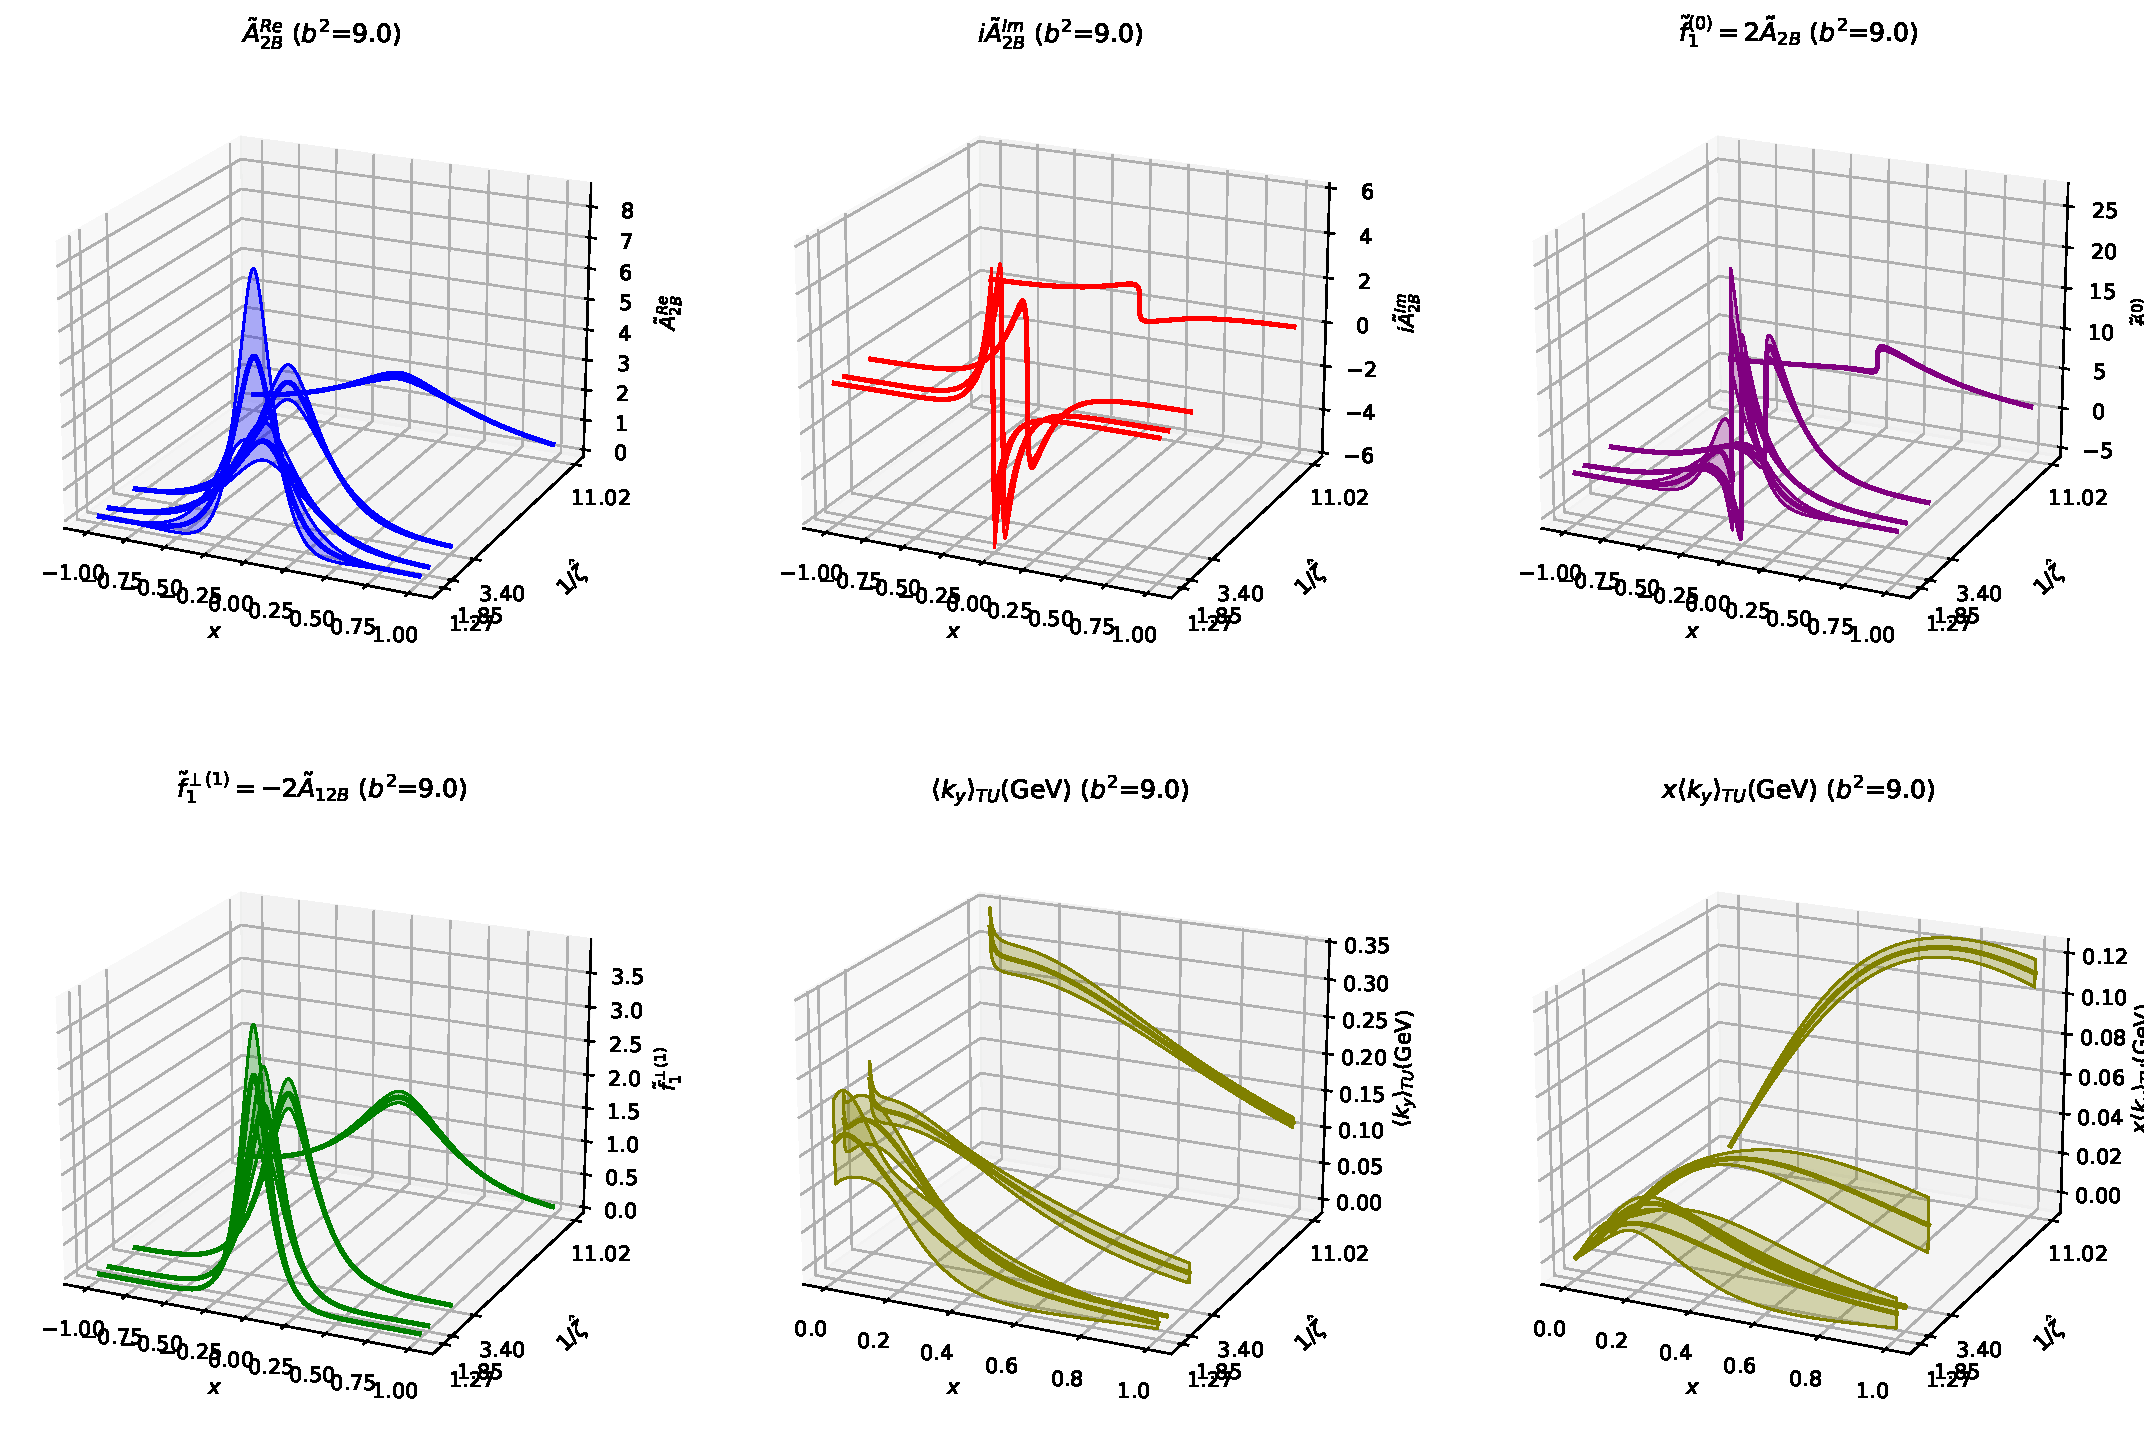
\includegraphics[width=0.8\linewidth]{SimultaneousFitsCov/SimulFit_Distinct_1_over_PL_bmin3_eta610_b29.0.pdf}
    \caption{Discrete $\hat\zeta$-slices of the reconstructed amplitudes, unpolarized and Sivers TMD combinations, and Sivers shift, plotted against both $x$ and $1/\hat\zeta$ at fixed transverse separation $|b_T| = 3a \approx 0.34$ fm. Each ribbon corresponds to one of the four simulated momenta $P_L = -1,-2,-3,-4$ (equivalently $1/\hat\zeta = 11.02,\ 3.40,\ 1.85,\ 1.27$). The systematic drift of every panel with $1/\hat\zeta$ motivates the extrapolation to the physical light-cone limit $\hat\zeta \to \infty$ performed below.}
    \label{fig:zetahat_discrete_slices}
\end{figure}

\subsection{Extrapolation at fit-parameters level}
\label{sec:extrap_fit_param_level}

The lowest simulated momentum, $P_L=-1$ ($\hat\zeta = 0.090772$), sits too close to the origin in $1/\hat\zeta$ to resolve the curvature required to anchor an extrapolation; including it risks biasing the fit away from the true asymptotic ($\hat\zeta \to \infty$) behavior rather than constraining it. We therefore exclude $P_L=-1$ and extrapolate using only the three higher, better-separated momenta $P_L = -2,-3,-4$.

Rather than extrapolate the amplitudes point by point in $x$, we extrapolate each of the twelve parameters of the global simultaneous-fit models directly: the four parameters $\{a,c,d,j\}$ appearing in each of the coupled Lorentzian models for $\tAmp_{2B}^{\text{Re}}$, $\tAmp_{2B}^{\text{Im}}$, and $\tAmp_{12B}^{\text{Re}}$ (Eq.~(\ref{eq:model_ReA2B})-(\ref{eq:model_ImA2B})). Following the kinematic scaling identified in Section~\ref{sec:fitting_methodologies}, the parameters $c_{\text{re}}$, $c_{\text{im}}$, and $c_{\text{reA12B}}$ are first rescaled by $1/P_L^2$ and $a_{\text{im}}$ by $1/P_L$, so that all three momenta can be fit on a common footing. For the resulting $\hat\zeta$-dependence of each rescaled parameter, we tested two functional forms,
\begin{equation}
    p(\hat\zeta) = c + \frac{d}{\hat\zeta} \qquad \text{and} \qquad p(\hat\zeta) = c + \frac{d}{\hat\zeta^2} \ ,
    \label{eq:zetahat_extrap_ansatz}
\end{equation}
using correlated Jackknife fits to the three data points. The quadratic ansatz consistently gave a lower $\chi^2/\text{dof}$ across the twelve parameters than the linear form and is adopted for every extrapolation shown below; the extrapolated, physical-limit value of each parameter is simply its fitted intercept $c$ at $1/\hat\zeta=0$.

\begin{figure}[h!]
    \centering
    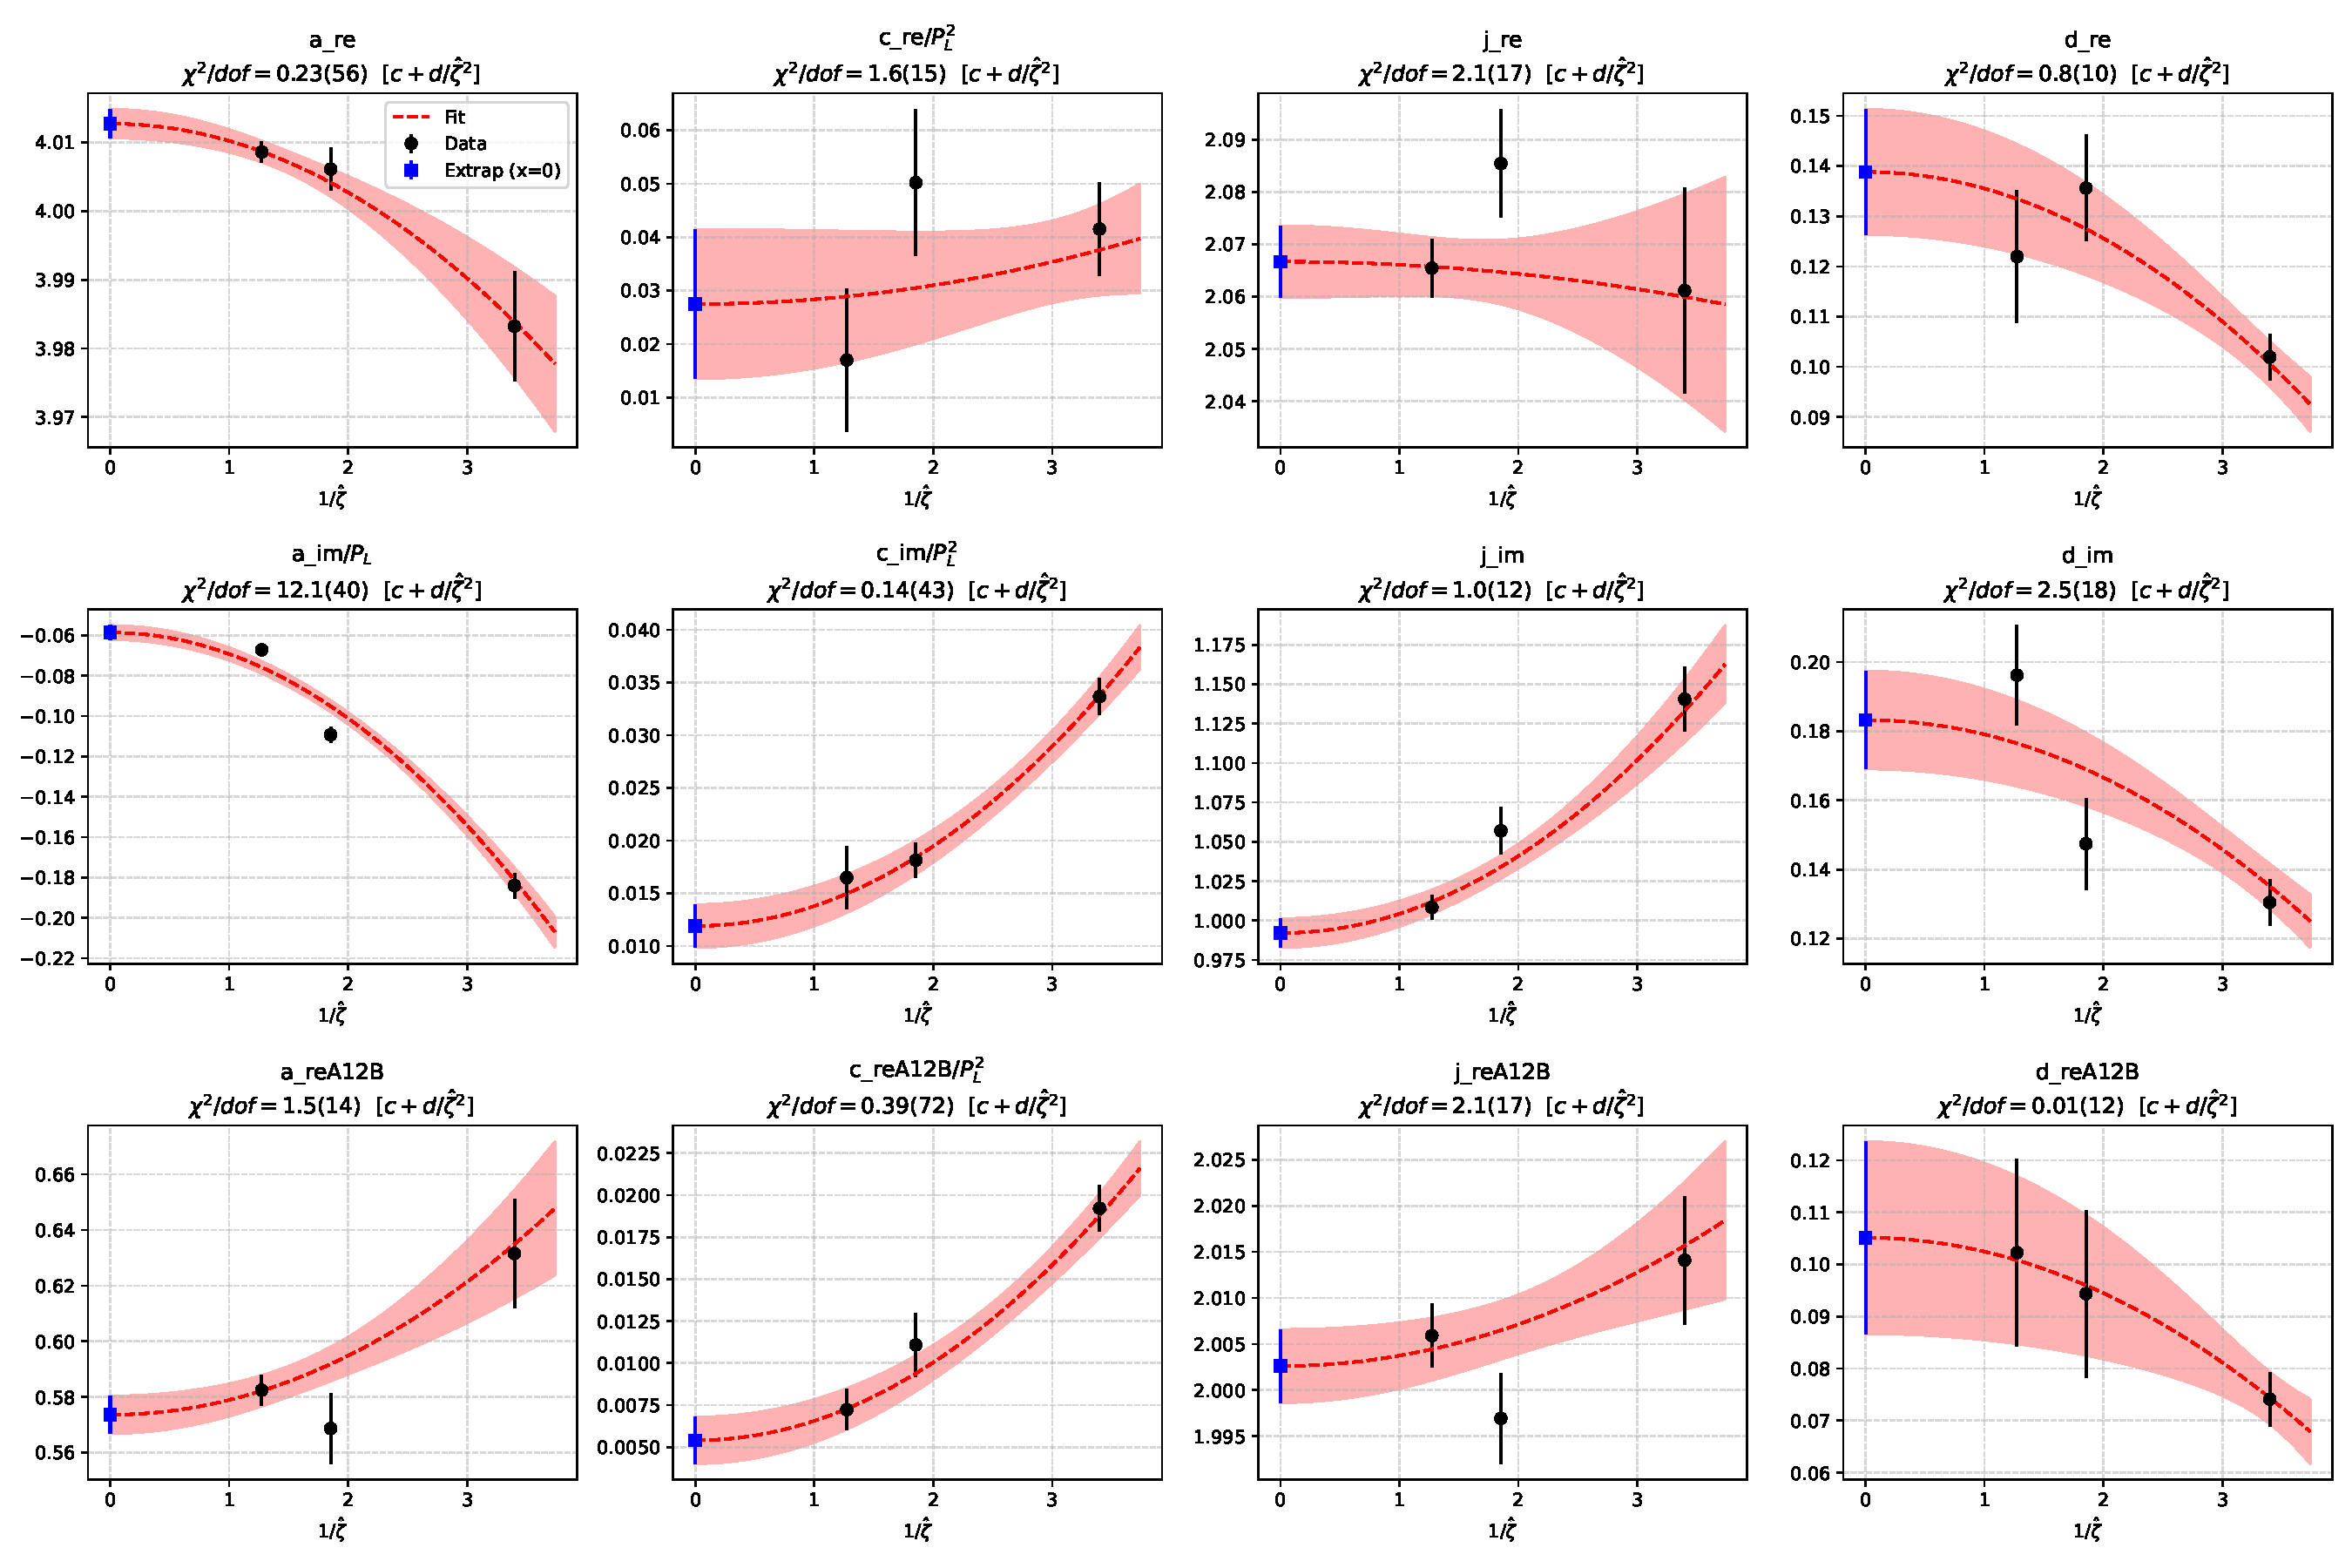
\includegraphics[width=0.8\linewidth]{SimultaneousFitsCov/extrapolation_para_level/Param_Extrapolations_1byZetahat_sq_P234_bmin3_eta610_b29.0.pdf}
    \caption{Extrapolation of the twelve simultaneous-fit parameters to the physical limit $\hat\zeta \to \infty$, using only the three higher momenta $P_L=-2,-3,-4$ (black points, plotted against $1/\hat\zeta$). The dashed red curve and shaded band show the fitted ansatz $c+d/\hat\zeta^2$ of Eq.~\ref{eq:zetahat_extrap_ansatz}, with each panel's Jackknife $\chi^2/\text{dof}$ noted in its title; the blue square at $1/\hat\zeta=0$ marks the extrapolated physical-limit value. The parameters $c_{\text{re}}$, $c_{\text{im}}$, and $c_{\text{reA12B}}$ are shown rescaled by $1/P_L^2$, and $a_{\text{im}}$ by $1/P_L$, as described in the text.}
    \label{fig:param_extrapolation_zetahat}
\end{figure}

Reconstructing the amplitudes from these twelve extrapolated parameters gives the unpolarized and Sivers TMD combinations directly at the physical limit, shown in Fig.~\ref{fig:extrapolated_amplitude_level} as continuous functions of $x$ at fixed $|b_T| = 3a \approx 0.34$ fm.

\begin{figure}[h!]
    \centering
    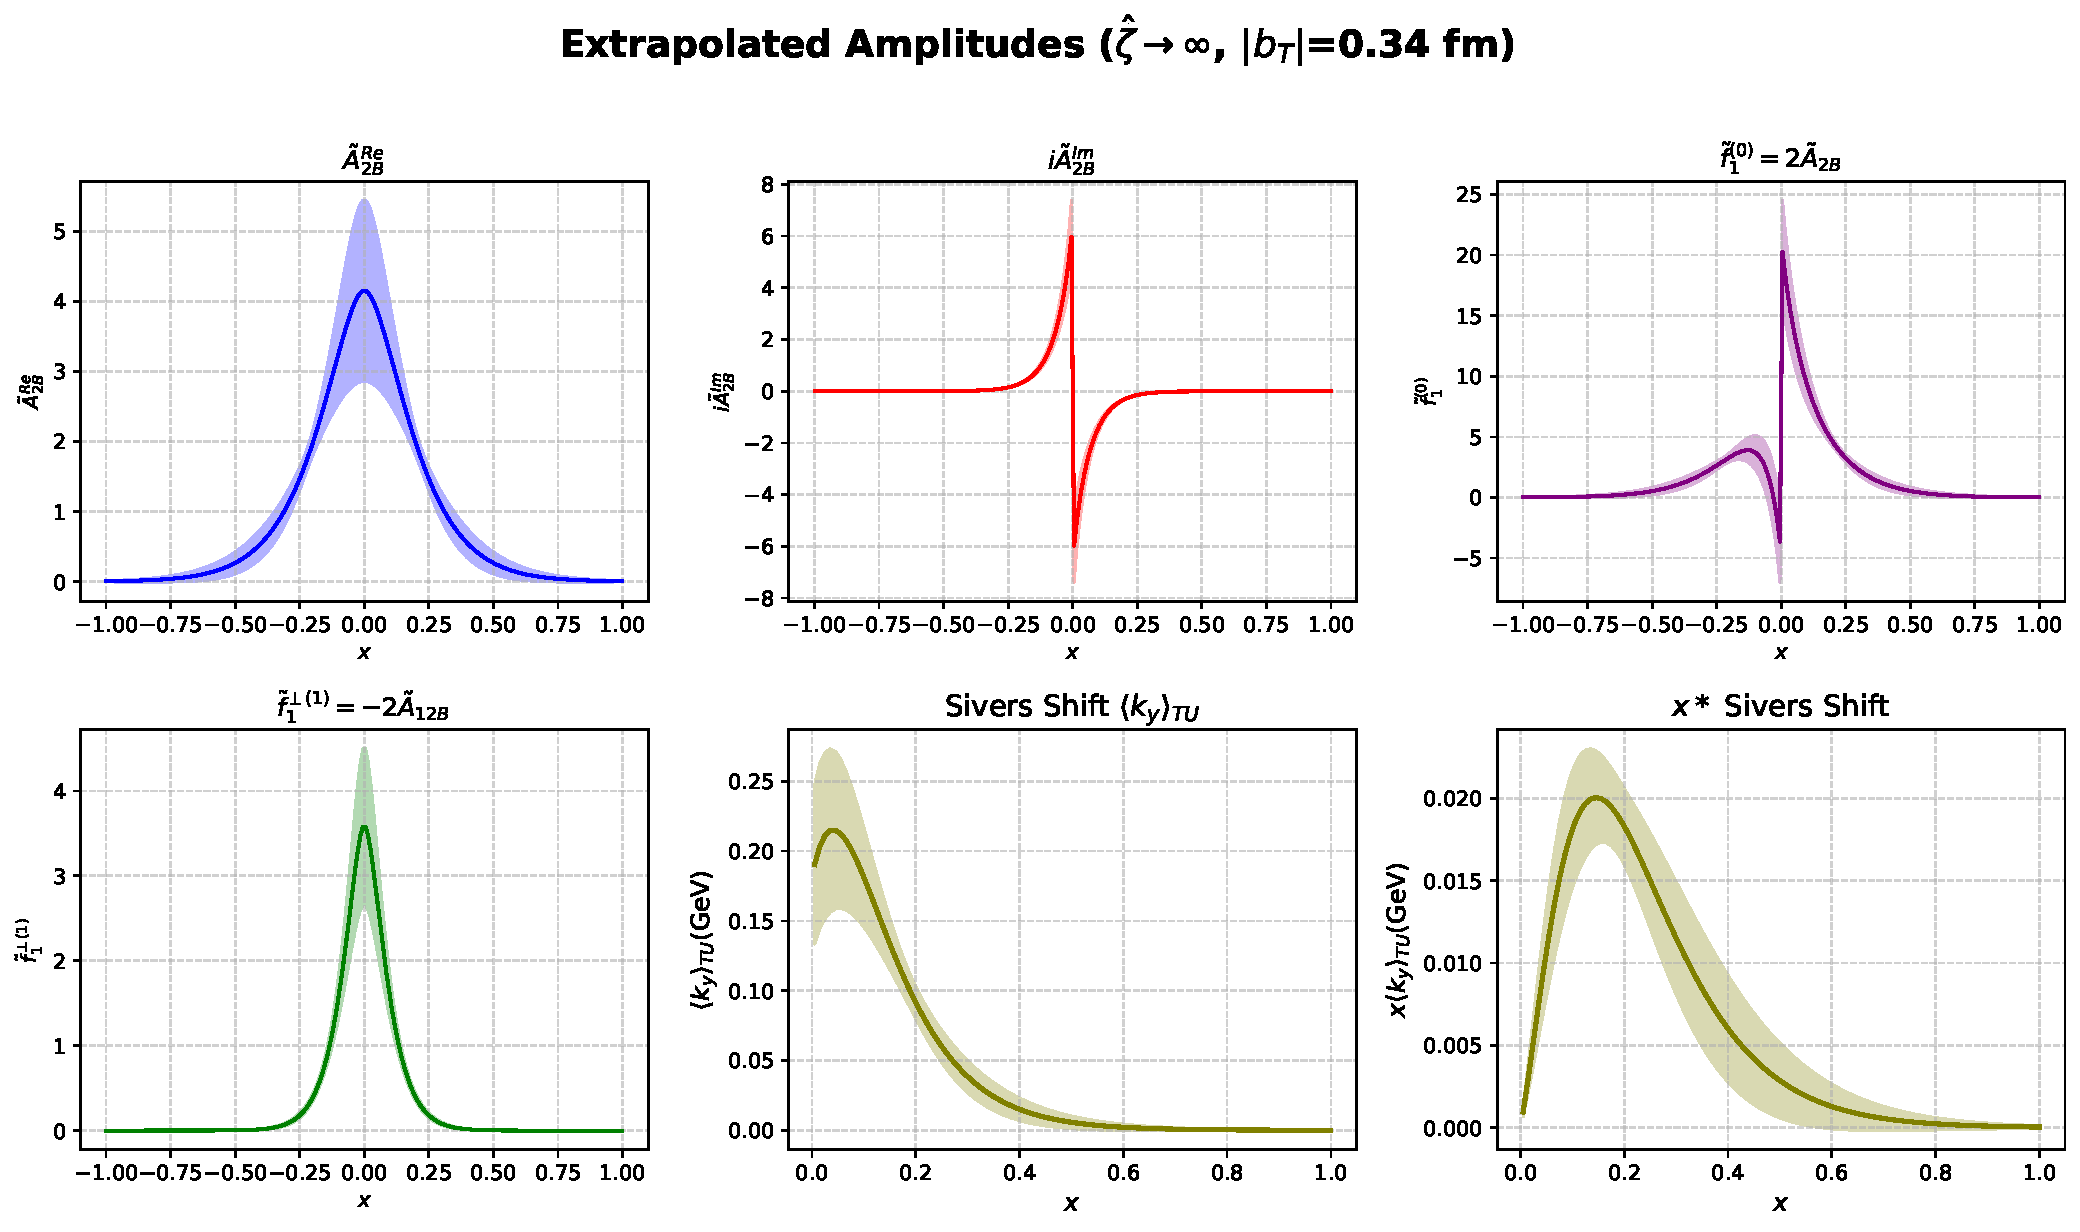
\includegraphics[width=0.8\linewidth]{SimultaneousFitsCov/extrapolation_para_level/Extrapolated_AmpLevel_P234_Sivers_1_over_zetahat_sq_bmin3_eta610_b29.0.pdf}
    \caption{Unpolarized and Sivers TMD amplitudes reconstructed from the extrapolated ($\hat\zeta\to\infty$) fit parameters of Fig.~\ref{fig:param_extrapolation_zetahat}, evaluated as continuous functions of $x$ at fixed transverse separation $|b_T| = 3a \approx 0.34$ fm: $\tAmp_{2B}^{\text{Re}}$, $i\tAmp_{2B}^{\text{Im}}$, the full unpolarized combination $\tilde f_1^{(0)}=2\tAmp_{2B}$, the Sivers combination $\tilde f_1^{\perp(1)}=-2\tAmp_{12B}^{\text{Re}}$, and the resulting Sivers shift $\langle k_y \rangle_{TU}$ and $x\langle k_y \rangle_{TU}$, the latter two restricted to the quark region $x\ge0$. Shaded bands are the Jackknife uncertainty propagated from the twelve extrapolated parameters.}
    \label{fig:extrapolated_amplitude_level}
\end{figure}

Table~\ref{tab:numerical_integration_fourier} lists the corresponding numerical Fourier-transform integrals at $|b_T|=3a\approx0.34$ fm, evaluated over the full range $x\in\{-\infty,\infty\}$ as well as the restricted ranges $\{-1,1\}$, $\{-1,0\}$, and $\{0,1\}$ used to isolate, respectively, the quark-plus-antiquark, antiquark, and quark contributions to the $x$-moments $\tilde f_1^{[1](0)}$ and $\tilde f_{1T}^{\perp[1](1)}$.

\begin{table}[h!]
    \centering
    \renewcommand{\arraystretch}{1.5}
    \caption{Numerical integration of the Fourier-transform integrals at $|b_T| = 3a \approx 0.34$ fm, evaluated using the extrapolated ($\hat\zeta\to\infty$) amplitudes of Fig.~\ref{fig:extrapolated_amplitude_level}, over the full range and three restricted $x$-ranges isolating the quark, antiquark, and combined contributions.}
    \label{tab:numerical_integration_fourier}
    \resizebox{\textwidth}{!}{%
    \begin{tabular}{|l|c|c|c|c|}
    \hline
    Integral & $\{-\infty,\infty\}$ & $\{-1,1\}$ & $\{-1,0\}$ & $\{0,1\}$ \\
    \hline
    $\displaystyle\int dx\, \tAmp_{2B}^{\text{Re}}$ & $1.88(20)$ & $1.88(20)$ & $0.941(100)$ & $0.941(100)$ \\
    \hline
    $\displaystyle\int dx\, (i\tAmp_{2B}^{\text{Im}})$ & $2(23)\times10^{-16}$ & $7(52)\times10^{-16}$ & $0.413(68)$ & $-0.423(72)$ \\
    \hline
    $\tilde f_1^{[1](0)} = 2\displaystyle\int dx\, (\tAmp_{2B}^{\text{Re}} - i\tAmp_{2B}^{\text{Im}})$ & $3.77(40)$ & $3.76(40)$ & $1.06(20)$ & $2.73(28)$ \\
    \hline
    $\tilde f_{1T}^{\perp[1](1)} = -2\displaystyle\int dx\, \tAmp_{12B}^{\text{Re}}$ & $0.76(13)$ & $0.76(13)$ & $0.379(67)$ & $0.379(67)$ \\
    \hline
    $\mN\,\dfrac{\tilde f_{1T}^{\perp[1](1)}}{\tilde f_1^{[1](0)}}$ & $0.217(38)$ & $0.217(38)$ & $0.387(89)$ & $0.150(26)$ \\
    \hline
    \end{tabular}%
    }
\end{table}

Restricting the integration to $x\in\{-1,0\}$ or $\{0,1\}$ isolates the antiquark and quark contributions respectively; because $\tAmp_{2B}^{\text{Im}}$ is an odd function of $x$ while $\tAmp_{2B}^{\text{Re}}$ and $\tAmp_{12B}^{\text{Re}}$ are even, the antiquark and quark ranges give equal $\int dx\,\tAmp_{2B}^{\text{Re}}$ and $\int dx\,\tAmp_{12B}^{\text{Re}}$ but opposite-sign $\int dx\,(i\tAmp_{2B}^{\text{Im}})$, so that the combined $\{-1,1\}$ integral of the imaginary term is consistent with zero to within uncertainty. Integrating over the full range $\{-\infty,\infty\}$ agrees with the physically motivated range $\{-1,1\}$ well within uncertainties, confirming that the extrapolated amplitudes decay fast enough in $x$ for the light-cone-momentum-fraction cutoff to be a negligible truncation.

Figure~\ref{fig:extrapolated_amplitude_3d} extends this reconstruction to the full dependence on both $x$ and transverse separation, while Fig.~\ref{fig:momenta_vs_extrapolated} compares the extrapolated result directly against each of the three finite momenta used to obtain it.

\pagebreak
\begin{figure}[h!]
    \centering
    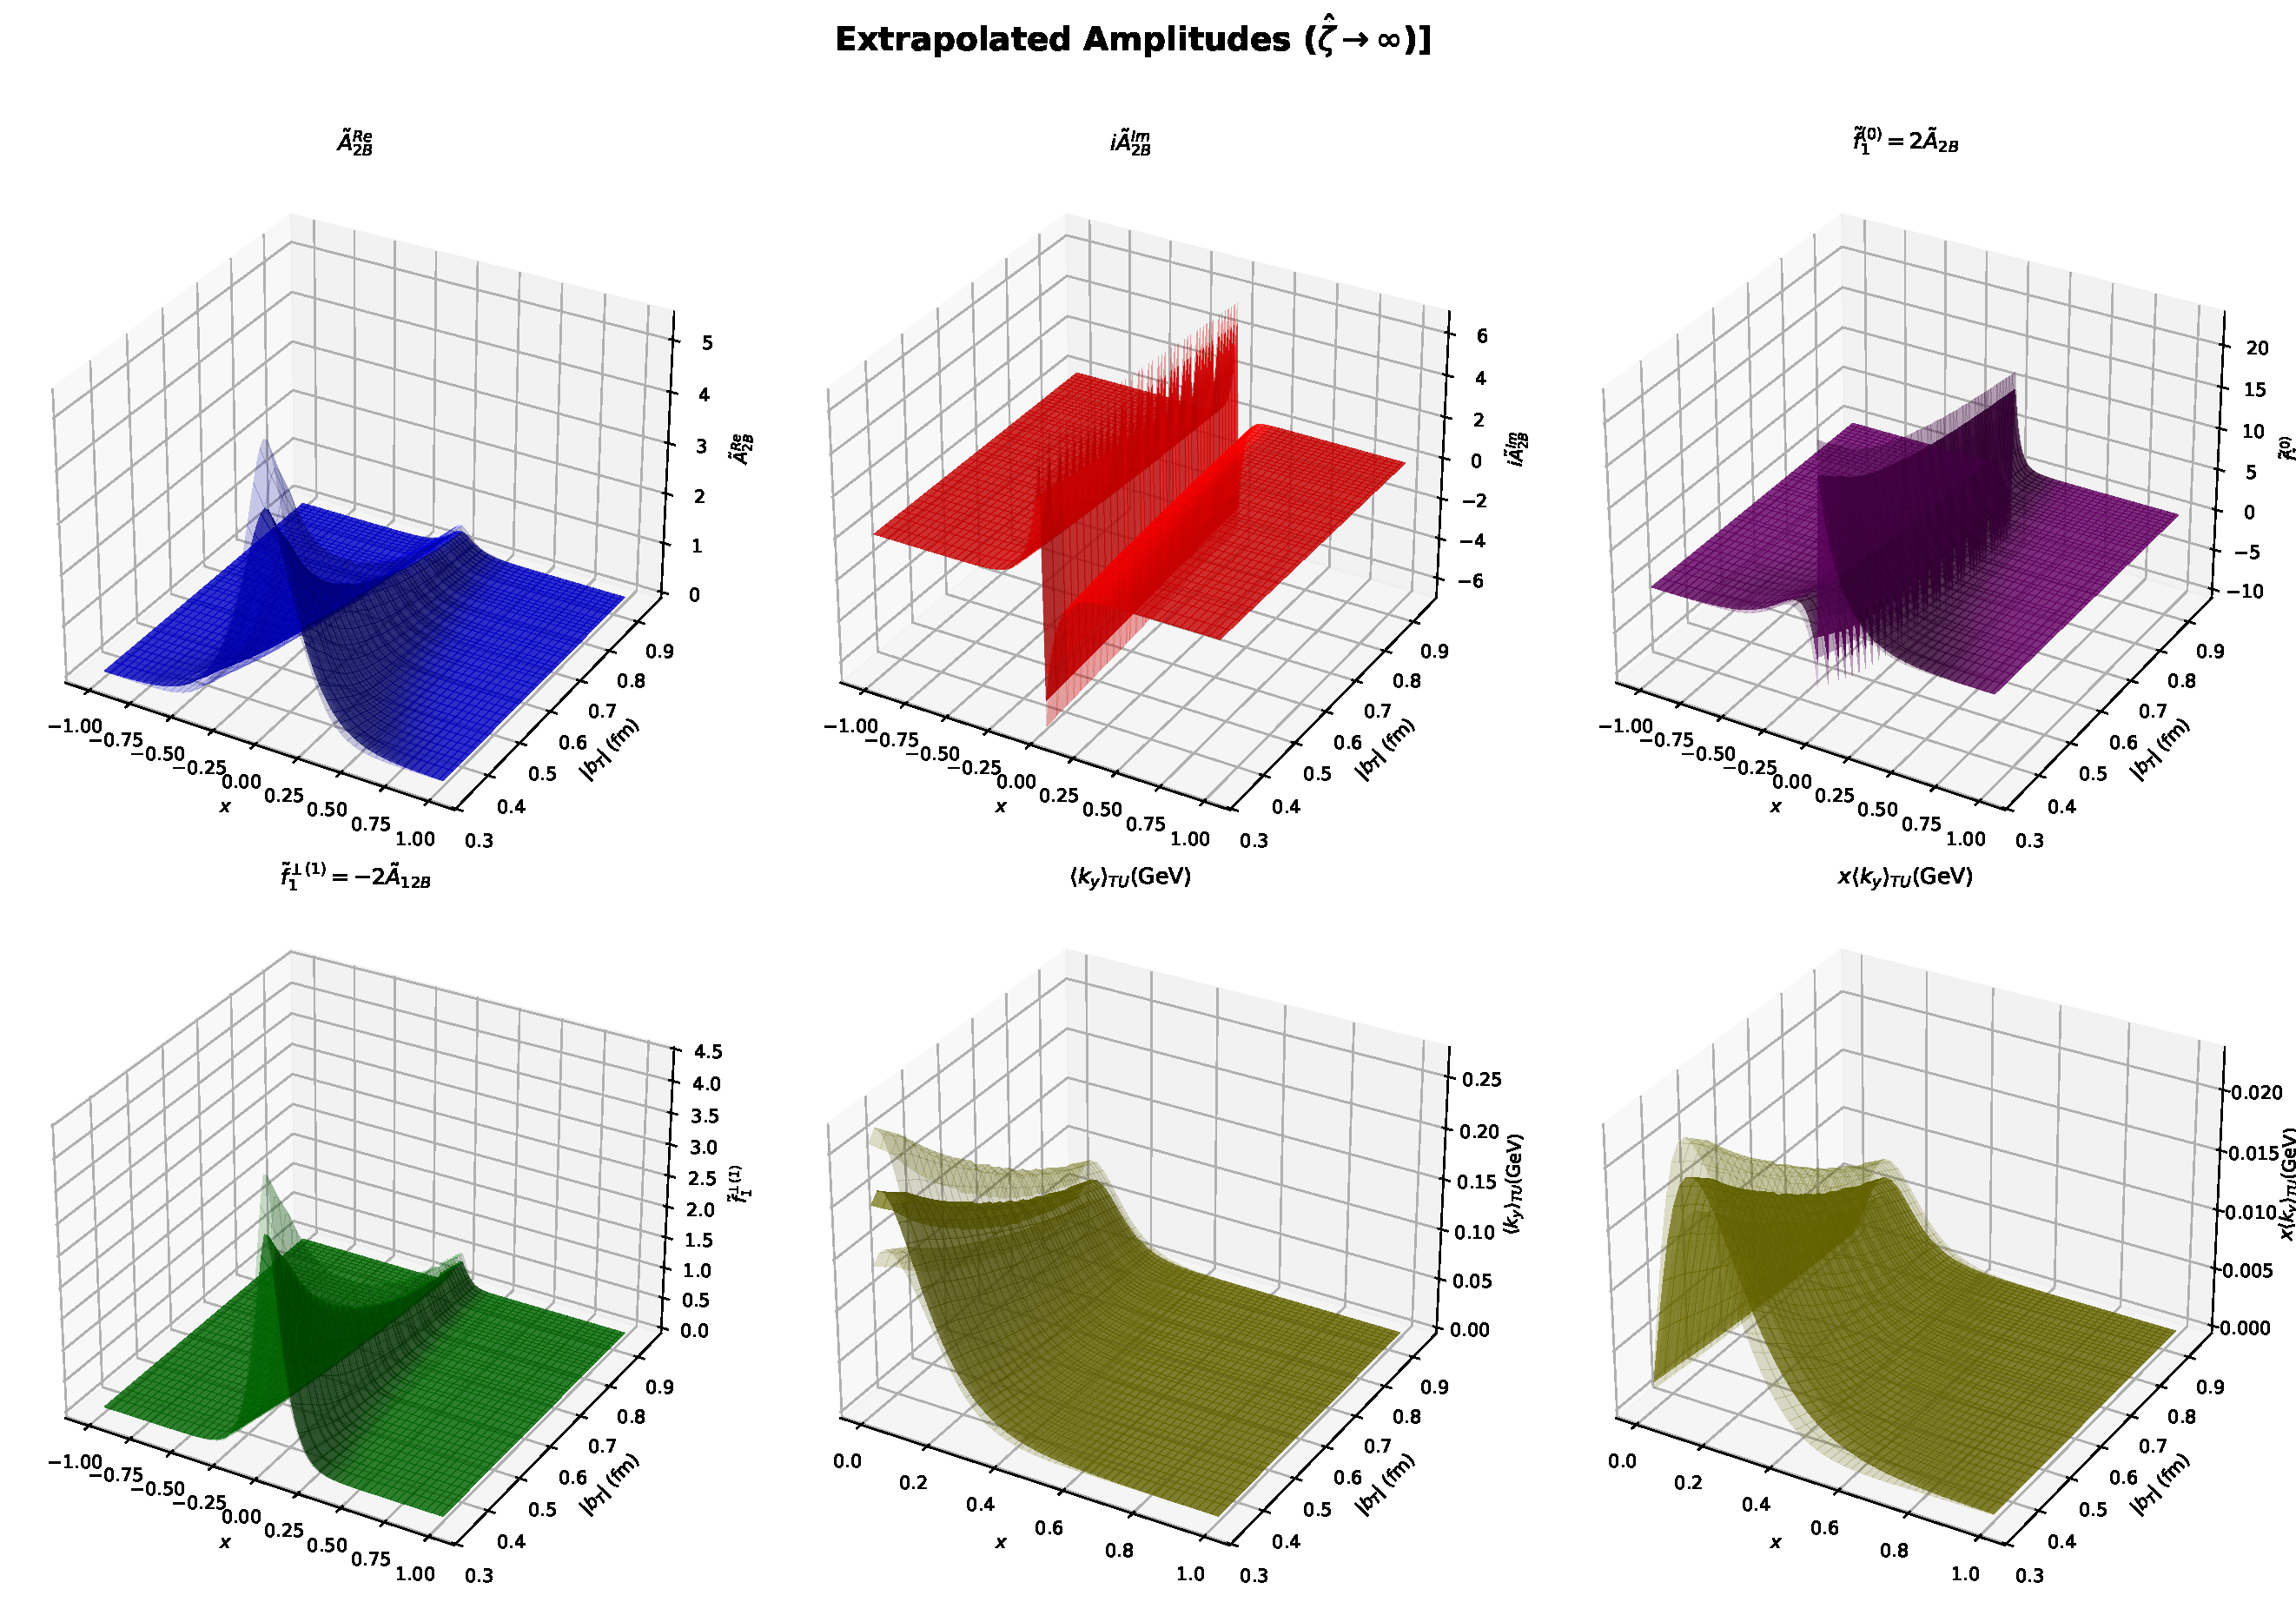
\includegraphics[width=0.8\linewidth]{SimultaneousFitsCov/extrapolation_para_level/SimulFitCovMatrix-A12B-A2B-FT-3D__bmin3_eta610_PLInf.pdf}
    \caption{The same six extrapolated ($\hat\zeta\to\infty$) quantities as Fig.~\ref{fig:extrapolated_amplitude_level}, shown here as full surfaces in $x$ and transverse separation $|b_T|$ (ranging from $3a\approx0.34$ fm to $\sqrt{68}\,a\approx0.94$ fm). The joint $x$-$|b_T|$ dependence illustrates how the reconstructed amplitudes and the extracted Sivers shift evolve with transverse quark separation at the physical limit.}
    \label{fig:extrapolated_amplitude_3d}
\end{figure}

\begin{figure}[h!]
    \centering
    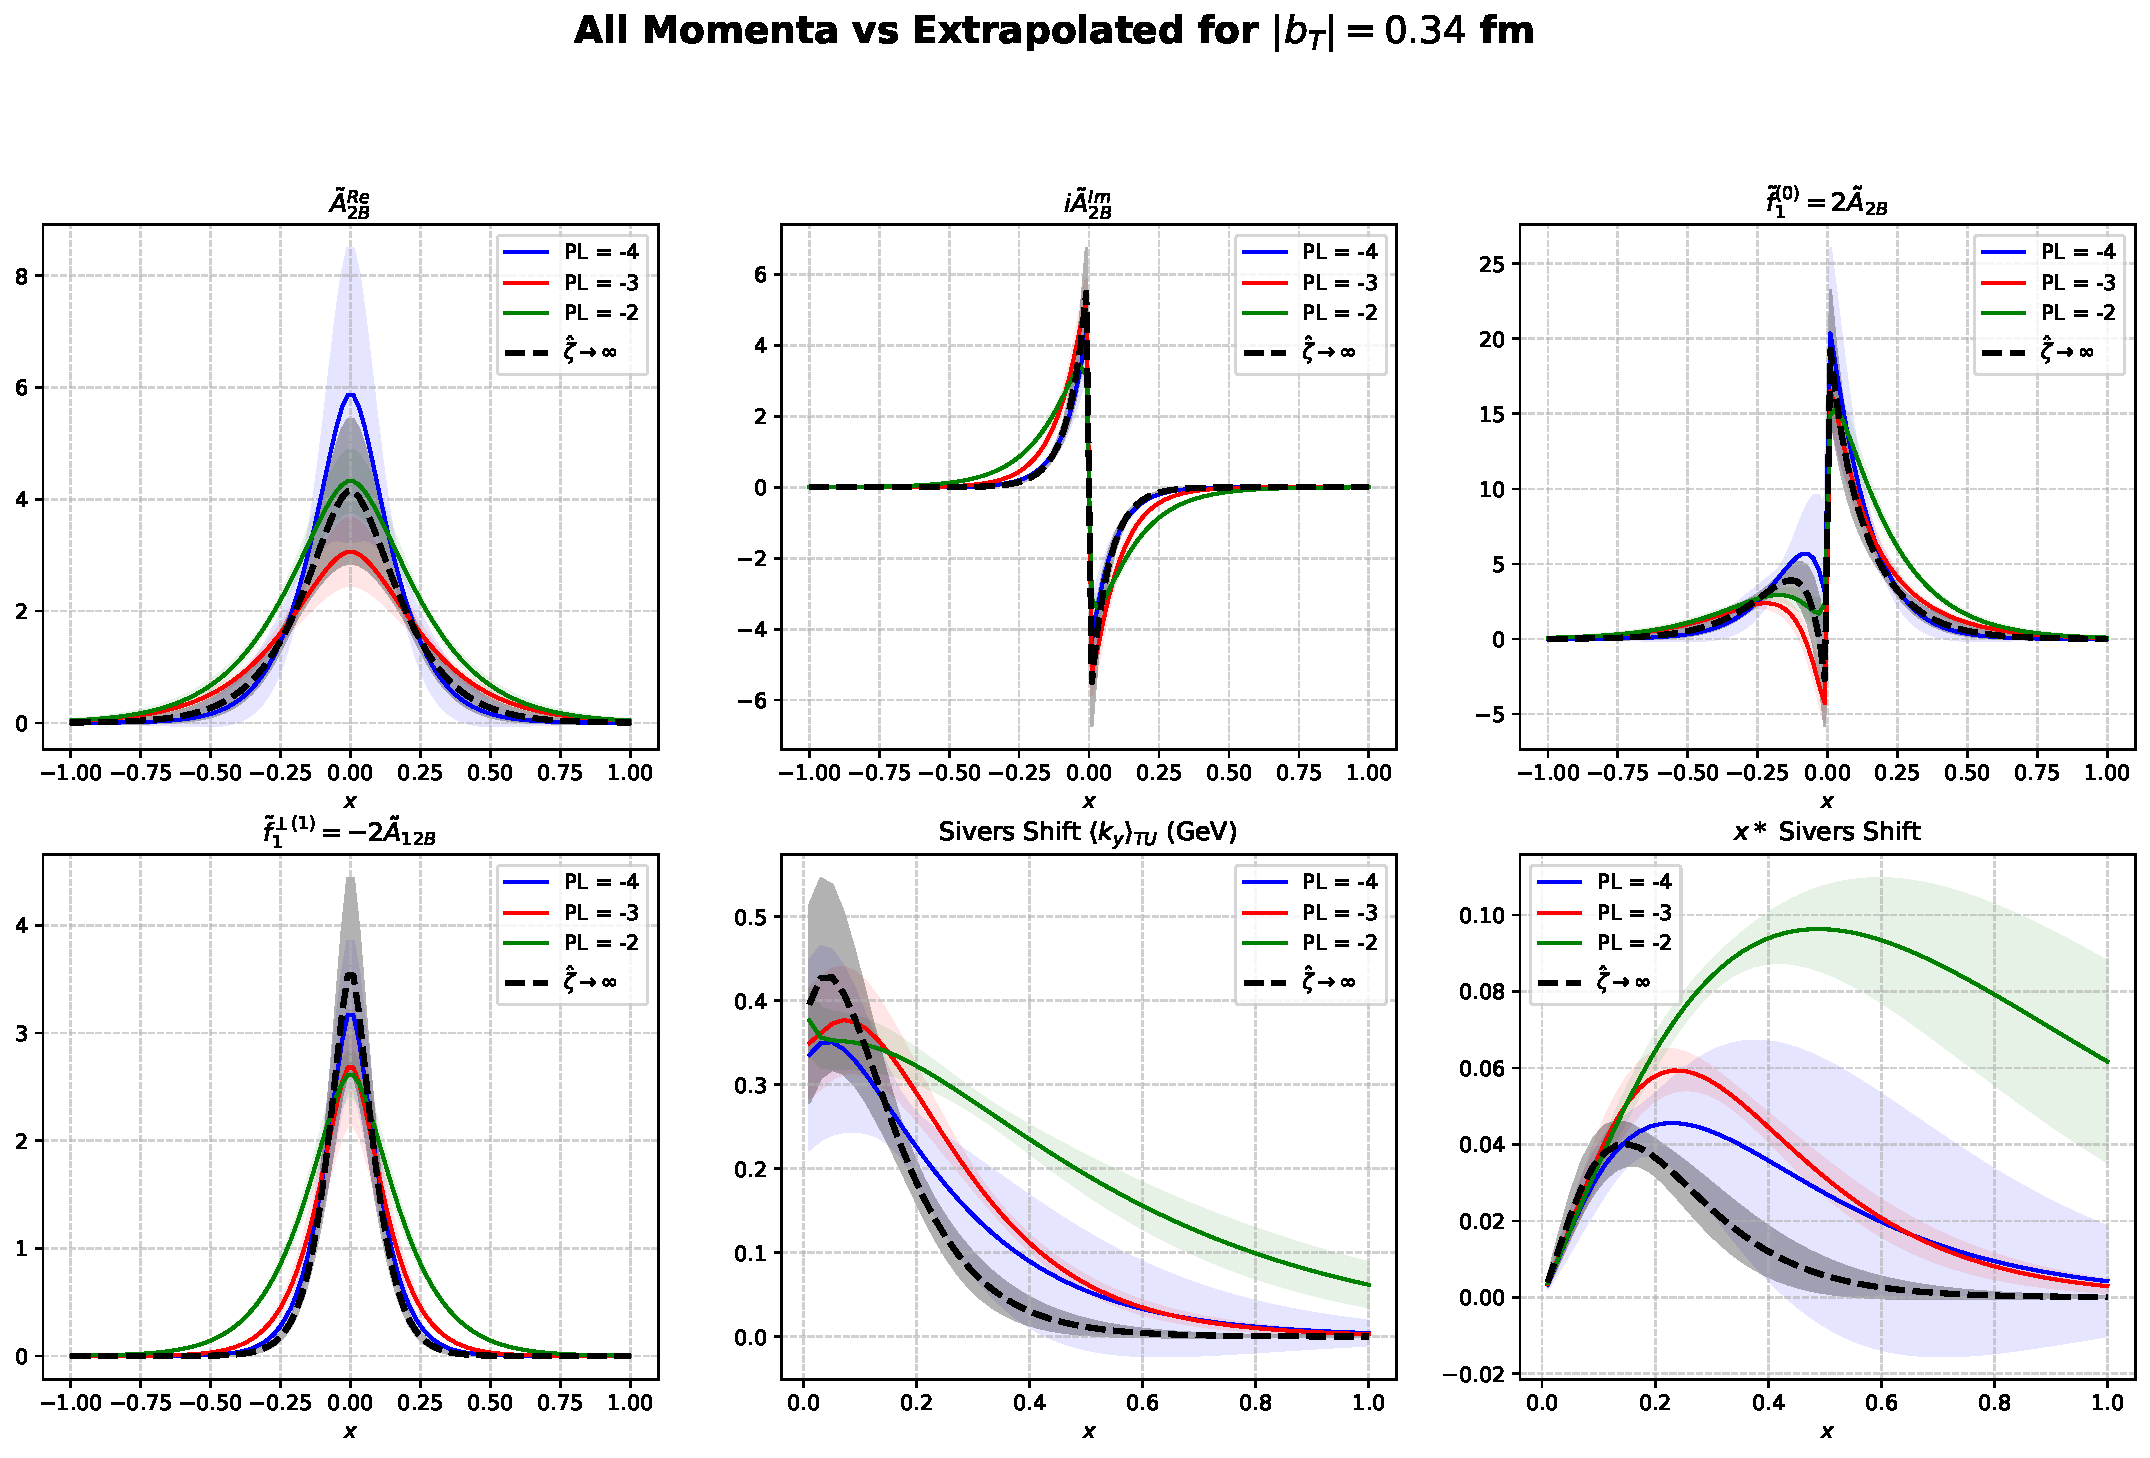
\includegraphics[width=0.8\linewidth]{SimultaneousFitsCov/extrapolation_para_level/All_Momenta_vs_Extrapolated_2D_P234_bmin3_eta610_b29.0.pdf}
    \caption{Comparison, at fixed $|b_T| = 3a \approx 0.34$ fm, between the six physical quantities evaluated at each of the three finite momenta used in the extrapolation ($P_L=-2,-3,-4$, colored curves, each using its own unextrapolated fit parameters) and the extrapolated $\hat\zeta\to\infty$ result (black dashed curve). The extrapolated curve is distinct from all three finite-momentum curves rather than coinciding with the largest simulated momentum, confirming that the fit-parameter extrapolation of Fig.~\ref{fig:param_extrapolation_zetahat} captures genuine momentum dependence rather than simply reproducing the $P_L=-4$ result.}
    \label{fig:momenta_vs_extrapolated}
\end{figure}

\subsection{Testing Factorization in \texorpdfstring{$x$}{TEXT} and \texorpdfstring{$|b_T|$}{TEXT}}
\label{sec:factorization_xbt}

Figures~\ref{fig:extrapolated_amplitude_3d} and~\ref{fig:momenta_vs_extrapolated} show that the extrapolated Sivers shift and amplitudes depend on both $x$ and $|b_T|$ jointly. A natural question is whether this joint dependence is actually separable: does the extrapolated Sivers shift factorize as
\begin{equation}
    \langle k_y \rangle_{TU}(x,|b_T|) \overset{?}{=} F(x)\,G(|b_T|) \ ,
\end{equation}
with all of the $x$-shape carried by $F(x)$ and all of the $|b_T|$-shape by $G(|b_T|)$? Such a factorization is not automatic in our fit ansatz. Each amplitude enters only through the combination $d_X(b^2) = 1 + d_X\,b^2$ inside a Bessel function that also carries the $x$-dependence,
\begin{equation}
    \tAmp_X(x,b^2) \ \propto\ N_X(b^2)\ |x|^{-1/2+j_X}\ K_{\nu_X}\!\left(|x|\sqrt{d_X(b^2)/c_X}\right) \ ,
\end{equation}
so $|b_T|$ rescales the argument of the same Bessel function that carries the $x$-dependence, rather than multiplying it by an overall $x$-independent prefactor. The Sivers shift is a ratio of three such amplitudes ($\tAmp_{2B}^{\text{Re}}$, $\tAmp_{2B}^{\text{Im}}$, $\tAmp_{12B}^{\text{Re}}$), each with its own independently fitted $(j_X,d_X)$; an exact factorization would require these parameters to coincide across the three amplitudes so that the $x$- and $|b_T|$-dependence separates cleanly. Whether the extrapolated fit lands close enough to that coincidence is a numerical question, which we answer quantitatively below.

\subsubsection{Quantifying the Distance from a Factorized Form}
\label{sec:factorization_metric}

Given a function of two variables $f(x,|b_T|)$, we quantify how far it is from a factorized form $g(x)h(|b_T|)$ by finding the closest such pair in the least-squares sense and reporting the residual. Explicitly, we minimize
\begin{equation}
    J = \int dx\, d|b_T| \, \big(f(x,|b_T|) - g(x)h(|b_T|)\big)^2
\end{equation}
over all functions $g$ and $h$. Setting the functional derivatives with respect to $g(x)$ and $h(|b_T|)$ to zero gives
\begin{align}
    0 &= \frac{\delta J}{\delta g(x)} = \int d|b_T|\, f(x,|b_T|)\,h(|b_T|) - g(x)\int d|b_T|\, h^2(|b_T|) \ , \\
    0 &= \frac{\delta J}{\delta h(|b_T|)} = \int dx\, f(x,|b_T|)\,g(x) - h(|b_T|)\int dx\, g^2(x) \ ,
\end{align}
which can be solved for $h$ in terms of $g$,
\begin{equation}
    h(|b_T|) = \frac{\int dx\, f(x,|b_T|)\,g(x)}{\int dx\, g^2(x)} \ ,
    \label{eq:factorization_h_solution}
\end{equation}
and reinserted to eliminate $h$, giving a closed, self-consistent equation for $g$ alone:
\begin{equation}
    g(x) = \left[\int d|b_T| \left[\frac{\int dx'\, f(x',|b_T|)\,g(x')}{\int dx'\, g^2(x')}\right]^2\right]^{-1} \int d|b_T|\, f(x,|b_T|)\,\frac{\int dx'\, f(x',|b_T|)\,g(x')}{\int dx'\, g^2(x')} \ .
    \label{eq:factorization_g_selfconsistent}
\end{equation}
Equation~\eqref{eq:factorization_g_selfconsistent} is solved iteratively: starting from an initial guess $g=1$, the right-hand side is evaluated to obtain a refined $g$, which is reinserted, and the process repeated until $g$ (and the resulting relative distance below) stops changing to within a fixed tolerance. Convergence is rapid in practice, typically within 4-6 iterations for the grids used here.

Having found the optimal separable pair $g(x)h(|b_T|)$, we compare its residual $\sqrt{J}$ to the overall size of $f$ itself, $N = \int dx\, d|b_T|\, f^2(x,|b_T|)$, giving the relative distance from a factorized form:
\begin{equation}
    \text{relative distance} = \sqrt{J/N} \ .
    \label{eq:factorization_relative_distance}
\end{equation}
A relative distance of zero indicates exact factorization; the closer to zero, the better $F(x)G(|b_T|)$ approximates the true joint $(x,|b_T|)$ dependence. In practice, we replace the continuum integrals with sums over a discrete $(x,|b_T|)$ grid, apply the iteration of Eq.~\eqref{eq:factorization_g_selfconsistent} independently to each Jackknife sample of the extrapolated amplitudes, and reduce the resulting distribution of relative distances to a Jackknife mean and error. We repeat the full test in four $x$-windows, $[0,1]$, $[0.1,0.9]$, $[0.2,0.8]$, and $[0.3,0.8]$, to check that the conclusion is not an artifact of the amplitudes' behavior near $x=0$.

\subsubsection{Factorization Test for the Sivers Shift}
\label{sec:factorization_sivers_test}

Before running the distance test itself, we can already see that exact factorization is unlikely from the extrapolated fit parameters directly. As noted in Section~\ref{sec:factorization_xbt}, factorization requires the Bessel-function order $j_X$ and width parameter $d_X$ to coincide across the three input amplitudes; the extrapolated values are
\begin{equation}
    j_{\text{re}} = 2.0667(69), \quad j_{\text{im}} = 0.9921(92), \quad j_{\text{reA12B}} = 2.0026(40) \ ,
\end{equation}
\begin{equation}
    d_{\text{re}} = 0.139(12), \quad d_{\text{im}} = 0.183(14), \quad d_{\text{reA12B}} = 0.105(18) \ .
\end{equation}
The two $j$ parameters entering the real amplitudes, $j_{\text{re}}$ and $j_{\text{reA12B}}$, agree with each other, but $j_{\text{im}} \approx 1$ is clearly distinct from both; the three $d$ parameters are closer to each other but still resolved from one another well outside their Jackknife uncertainties. This parameter-level mismatch, particularly in $j$, is a concrete, independent reason to expect a nonzero residual from exact factorization.

Table~\ref{tab:factorization_sivers} lists the resulting relative distance of the extrapolated Sivers shift $\langle k_y \rangle_{TU}(x,|b_T|)$ from its best separable approximation, over $|b_T| \in [0.3421,0.9403]$ fm (60 points, fixed across all four $x$-windows).

\begin{table}[h!]
    \centering
    \renewcommand{\arraystretch}{1.4}
    \caption{Relative distance of the extrapolated Sivers shift $\langle k_y \rangle_{TU}(x,|b_T|)$ from its optimal factorized approximation $F(x)G(|b_T|)$, Eq.~\eqref{eq:factorization_relative_distance}, over $|b_T| \in [0.3421, 0.9403]$ fm for four choices of $x$-window.}
    \label{tab:factorization_sivers}
    \begin{tabular}{|c|c|c|}
    \hline
    $x$-window & ALS iterations to converge & Relative distance \\
    \hline
    $[0.0,1.0]$ & 4 & $0.0568(78)$ \\
    \hline
    $[0.1,0.9]$ & 5 & $0.0714(95)$ \\
    \hline
    $[0.2,0.8]$ & 5 & $0.0758(75)$ \\
    \hline
    $[0.3,0.8]$ & 4 & $0.0620(88)$ \\
    \hline
    \end{tabular}
\end{table}

In every window the relative distance is nonzero well outside its Jackknife uncertainty, at the level of $6$-$8\%$: the Sivers shift is close to, but not exactly, factorized, and this residual is stable under narrowing the $x$-window away from $x=0$ rather than being driven by behavior at the endpoint. Figure~\ref{fig:factorization_gh_sivers} shows the resulting optimal separable factors $g(x)$ and $h(|b_T|)$ for all four windows together with the quality of the $g(x)h(|b_T|)$ reconstruction against the actual data at the two extreme $|b_T|$ values in the fit range.

\begin{figure}[h!]
    \centering
    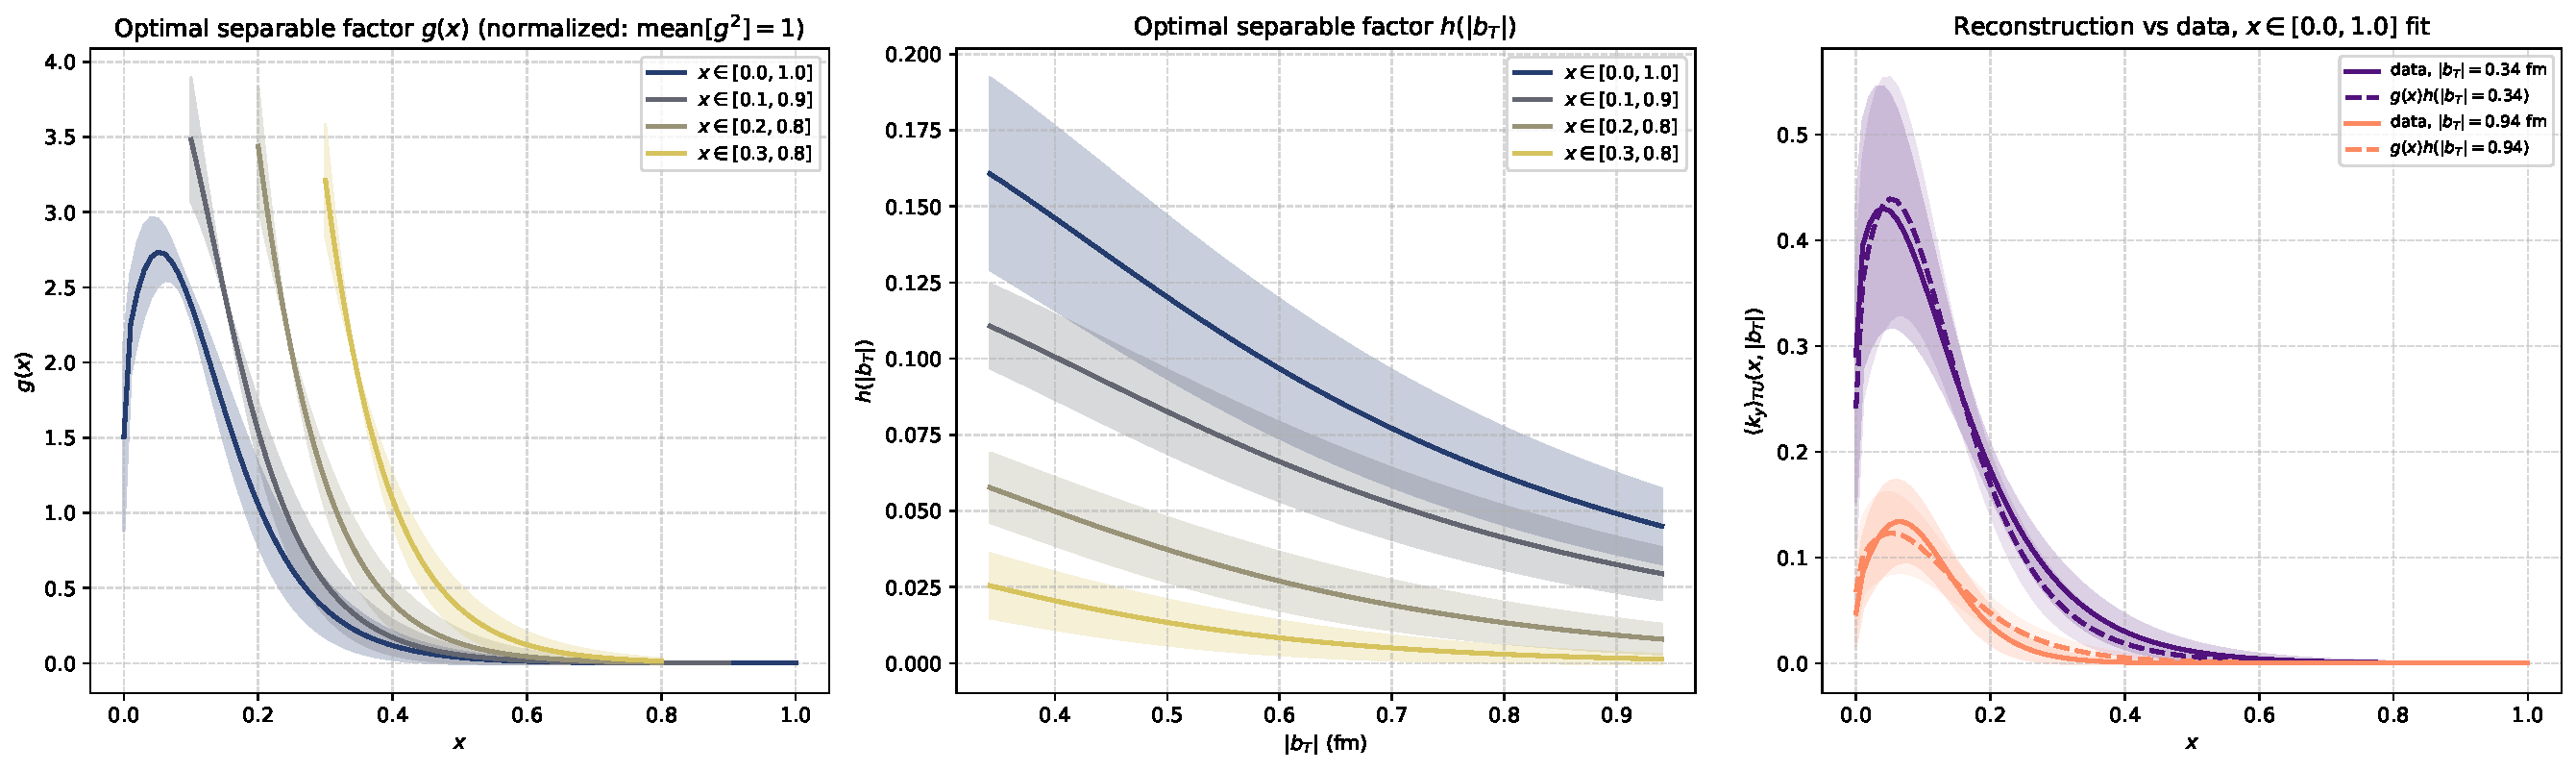
\includegraphics[width=\linewidth]{SimultaneousFitsCov/factorization_test/Factorization_gh_and_Reconstruction_bmin3_eta610.pdf}
    \caption{Left and center: the optimal separable factors $g(x)$ and $h(|b_T|)$ (Eqs.~\eqref{eq:factorization_h_solution}-\eqref{eq:factorization_g_selfconsistent}, normalized so $\text{mean}[g^2]=1$) for the extrapolated Sivers shift, shown for all four $x$-windows of Table~\ref{tab:factorization_sivers}. Right: the reconstructed $g(x)h(|b_T|)$ (dashed) compared to the actual extrapolated Sivers shift (solid) at the smallest and largest fitted $|b_T|$, using the $x\in[0,1]$ fit; the visible gap between the solid and dashed curves is the residual quantified in Table~\ref{tab:factorization_sivers}.}
    \label{fig:factorization_gh_sivers}
\end{figure}

A complementary, more direct way to see the same non-factorization is to form explicit ratios of the Sivers shift at fixed $x$ or fixed $|b_T|$. If $\langle k_y \rangle_{TU}(x,|b_T|) = F(x)G(|b_T|)$ exactly, then $R_b(x) \equiv \langle k_y \rangle_{TU}(x,|b_T|)/\langle k_y \rangle_{TU}(x,|b_T|_{\text{ref}}) = G(|b_T|)/G(|b_T|_{\text{ref}})$ must be flat in $x$ for every choice of $|b_T|$ and reference $|b_T|_{\text{ref}}$, and likewise $R_x(|b_T|) \equiv \langle k_y \rangle_{TU}(x,|b_T|)/\langle k_y \rangle_{TU}(x_{\text{ref}},|b_T|) = F(x)/F(x_{\text{ref}})$ must be flat in $|b_T|$ for every $x$ and $x_{\text{ref}}$; requiring this for every pair of references is not just necessary but sufficient for factorization, so it is a complete test rather than a heuristic proxy. Figures~\ref{fig:factorization_ratio_x_sivers} and~\ref{fig:factorization_ratio_bT_sivers} show that neither ratio is flat.

\begin{figure}[h!]
    \centering
    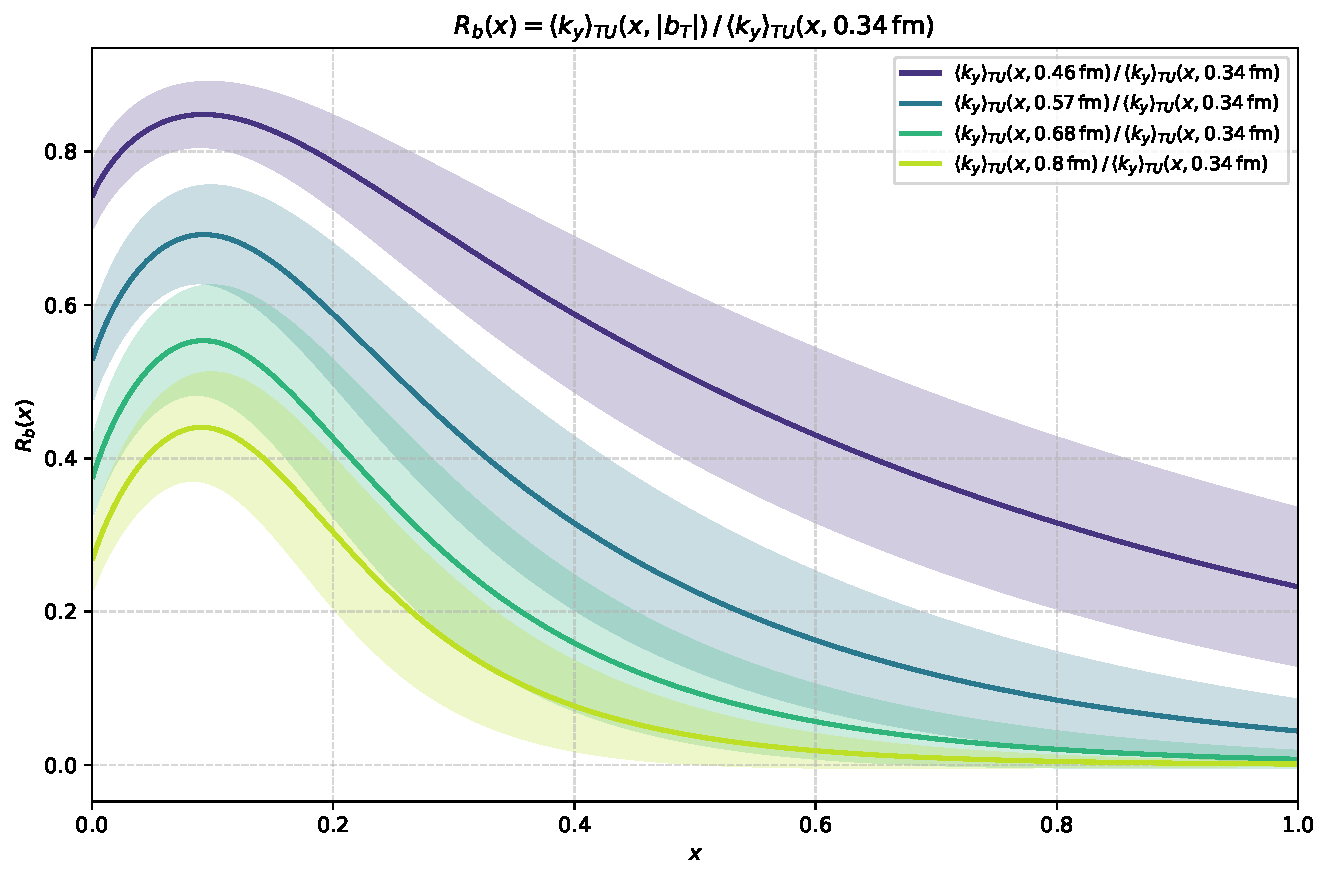
\includegraphics[width=0.75\linewidth]{SimultaneousFitsCov/factorization_test/Factorization_Ratio_vs_x_4curves_P234_bmin3_eta610.pdf}
    \caption{$R_b(x) = \langle k_y \rangle_{TU}(x,|b_T|)/\langle k_y \rangle_{TU}(x,0.34\text{ fm})$ for four values of $|b_T|$, as a function of $x$. Under exact factorization each curve would be flat; instead every curve rises from its $x\to0$ value to a peak near $x\approx0.1$ before decaying, showing that the $|b_T|$-dependence of the Sivers shift is itself $x$-dependent.}
    \label{fig:factorization_ratio_x_sivers}
\end{figure}

\begin{figure}[h!]
    \centering
    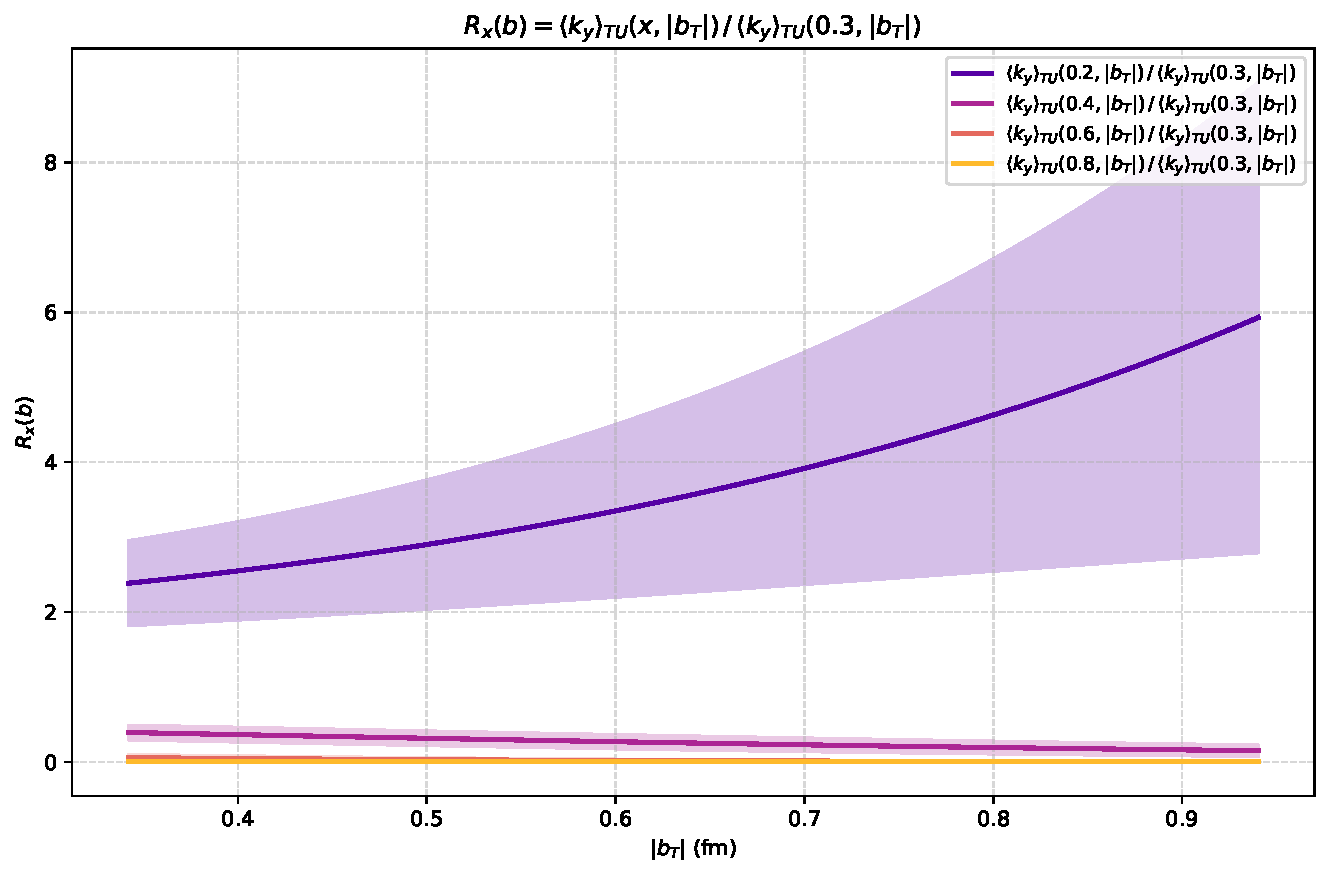
\includegraphics[width=0.75\linewidth]{SimultaneousFitsCov/factorization_test/Factorization_Ratio_vs_bT_4curves_P234_bmin3_eta610.pdf}
    \caption{$R_x(|b_T|) = \langle k_y \rangle_{TU}(x,|b_T|)/\langle k_y \rangle_{TU}(0.3,|b_T|)$ for four values of $x$, as a function of $|b_T|$. The $x=0.2$ curve varies by more than a factor of two across the fitted $|b_T|$ range rather than remaining flat, confirming that the $x$-dependence of the Sivers shift is itself $|b_T|$-dependent, consistent with Fig.~\ref{fig:factorization_ratio_x_sivers}.}
    \label{fig:factorization_ratio_bT_sivers}
\end{figure}

Finally, we check that this non-factorization is not an artifact introduced by the $\hat\zeta\to\infty$ extrapolation itself, by repeating the $R_b(x)$ and $R_x(|b_T|)$ ratio tests directly on the raw, unextrapolated fit parameters at each individual finite momentum. Figures~\ref{fig:factorization_ratio_x_finitePL} and~\ref{fig:factorization_ratio_bT_finitePL} show that the same qualitative pattern, non-flat ratios in both $x$ and $|b_T|$, is already present at every simulated momentum, and if anything becomes more pronounced at the higher momenta.

\begin{figure}[h!]
    \centering
    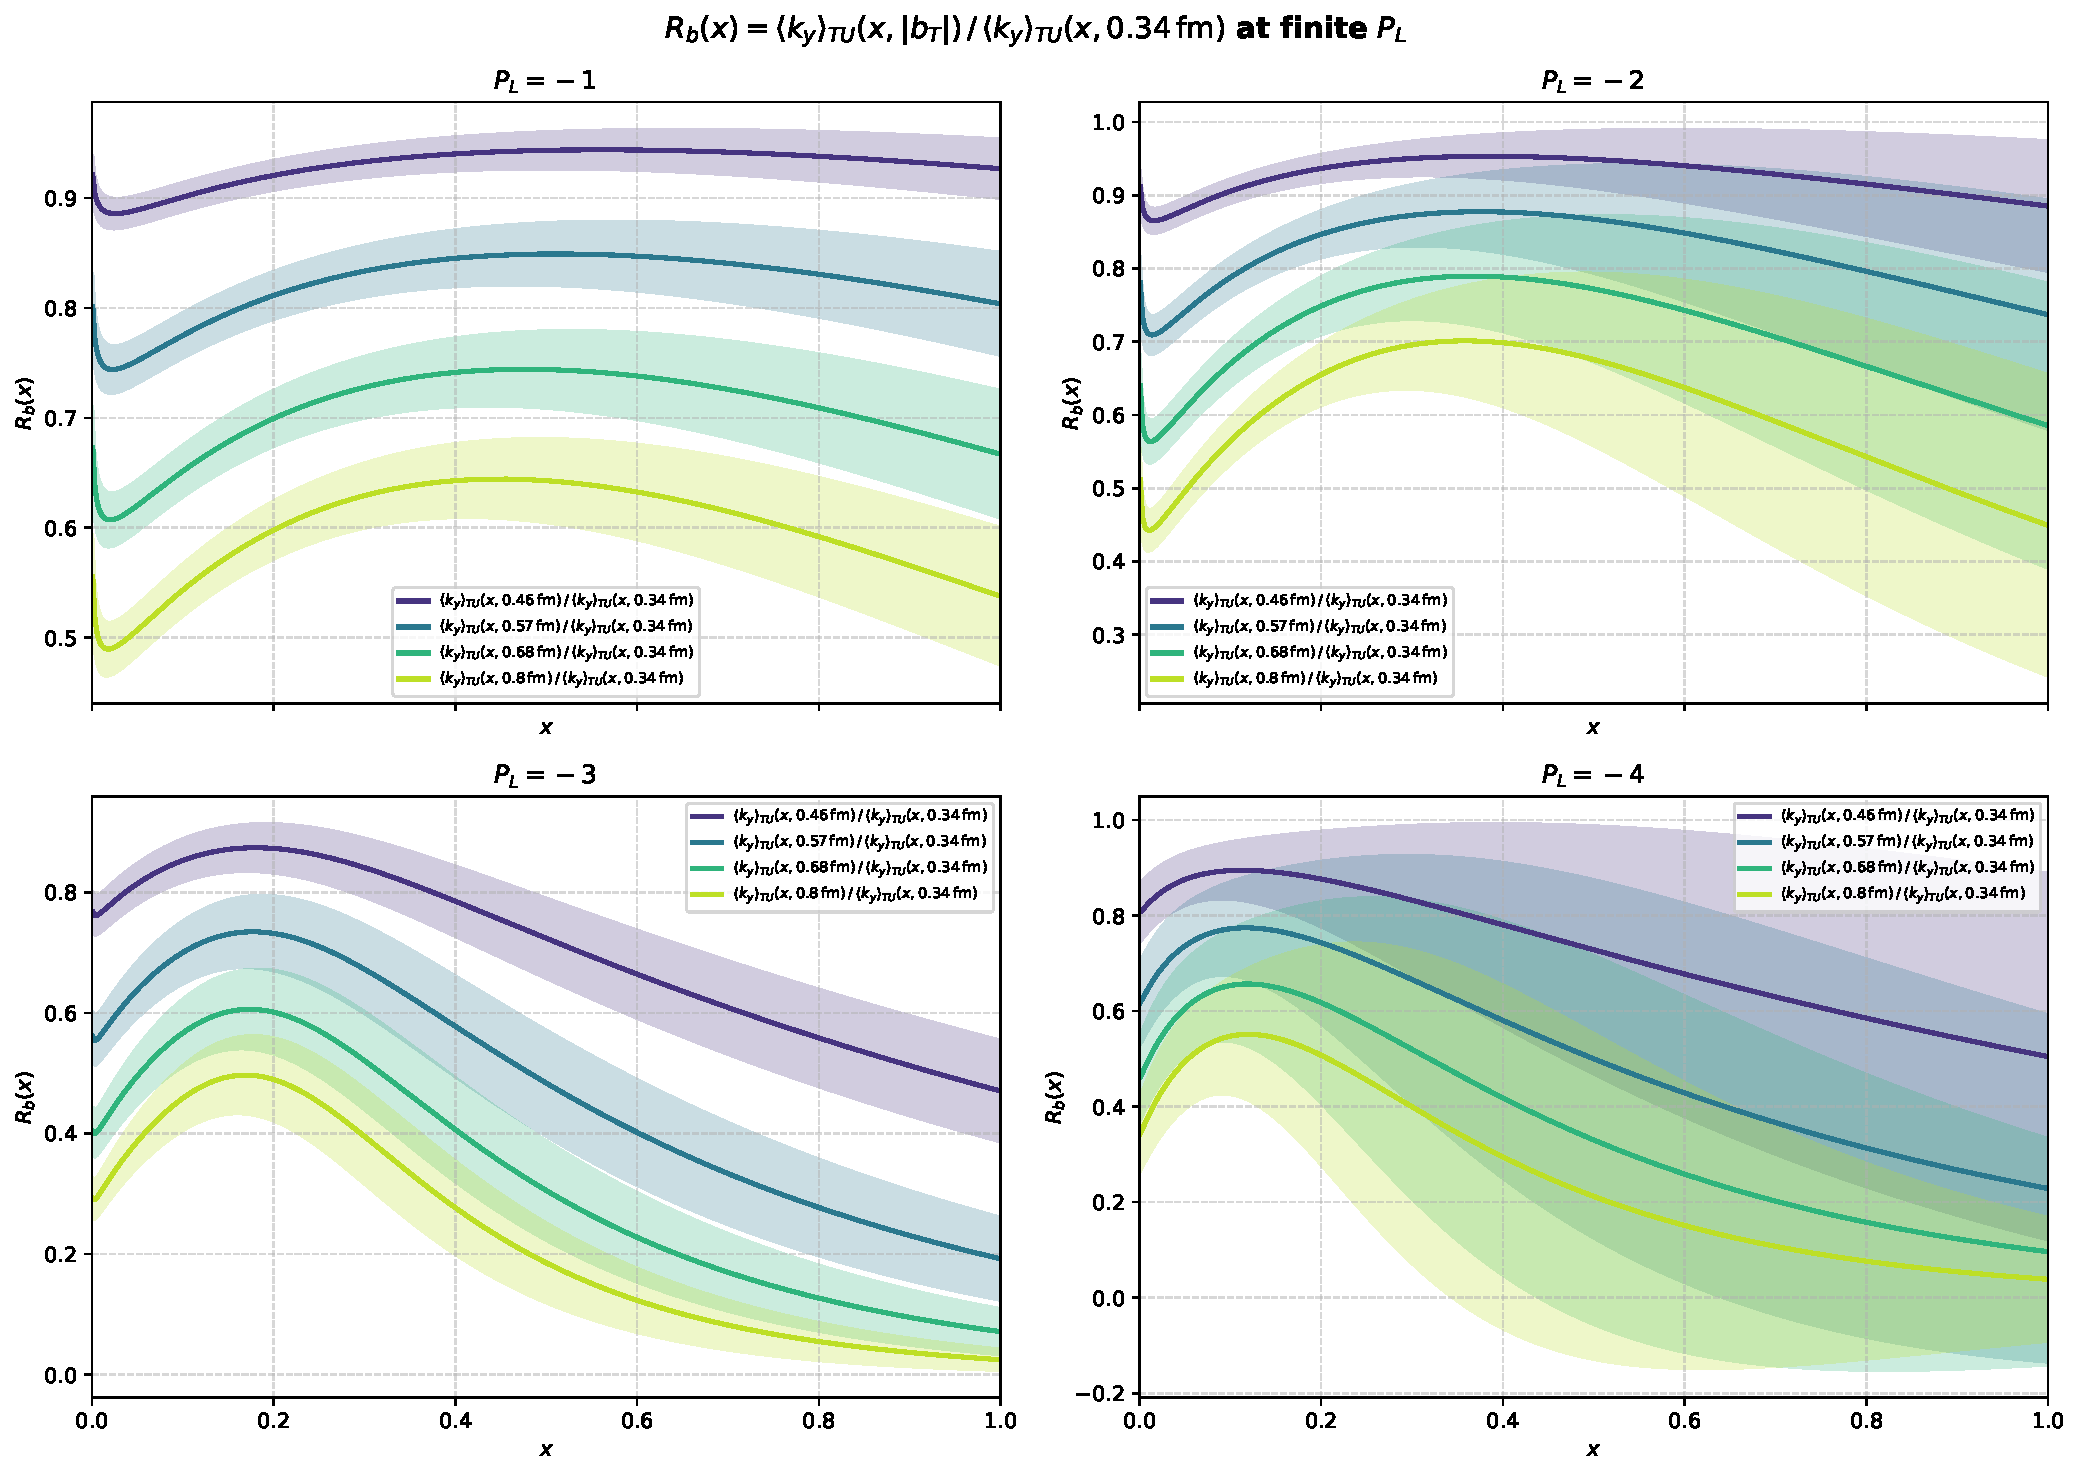
\includegraphics[width=\linewidth]{SimultaneousFitsCov/factorization_test/Factorization_Ratio_vs_x_AllPL_bmin3_eta610.pdf}
    \caption{The same ratio test as Fig.~\ref{fig:factorization_ratio_x_sivers}, $R_b(x)$, repeated at each finite momentum individually using its own raw (unextrapolated) fit parameters. None of the four panels shows a flat curve, confirming that the non-factorization is a genuine feature of the fitted amplitudes rather than an artifact of the $\hat\zeta\to\infty$ extrapolation.}
    \label{fig:factorization_ratio_x_finitePL}
\end{figure}

\begin{figure}[h!]
    \centering
    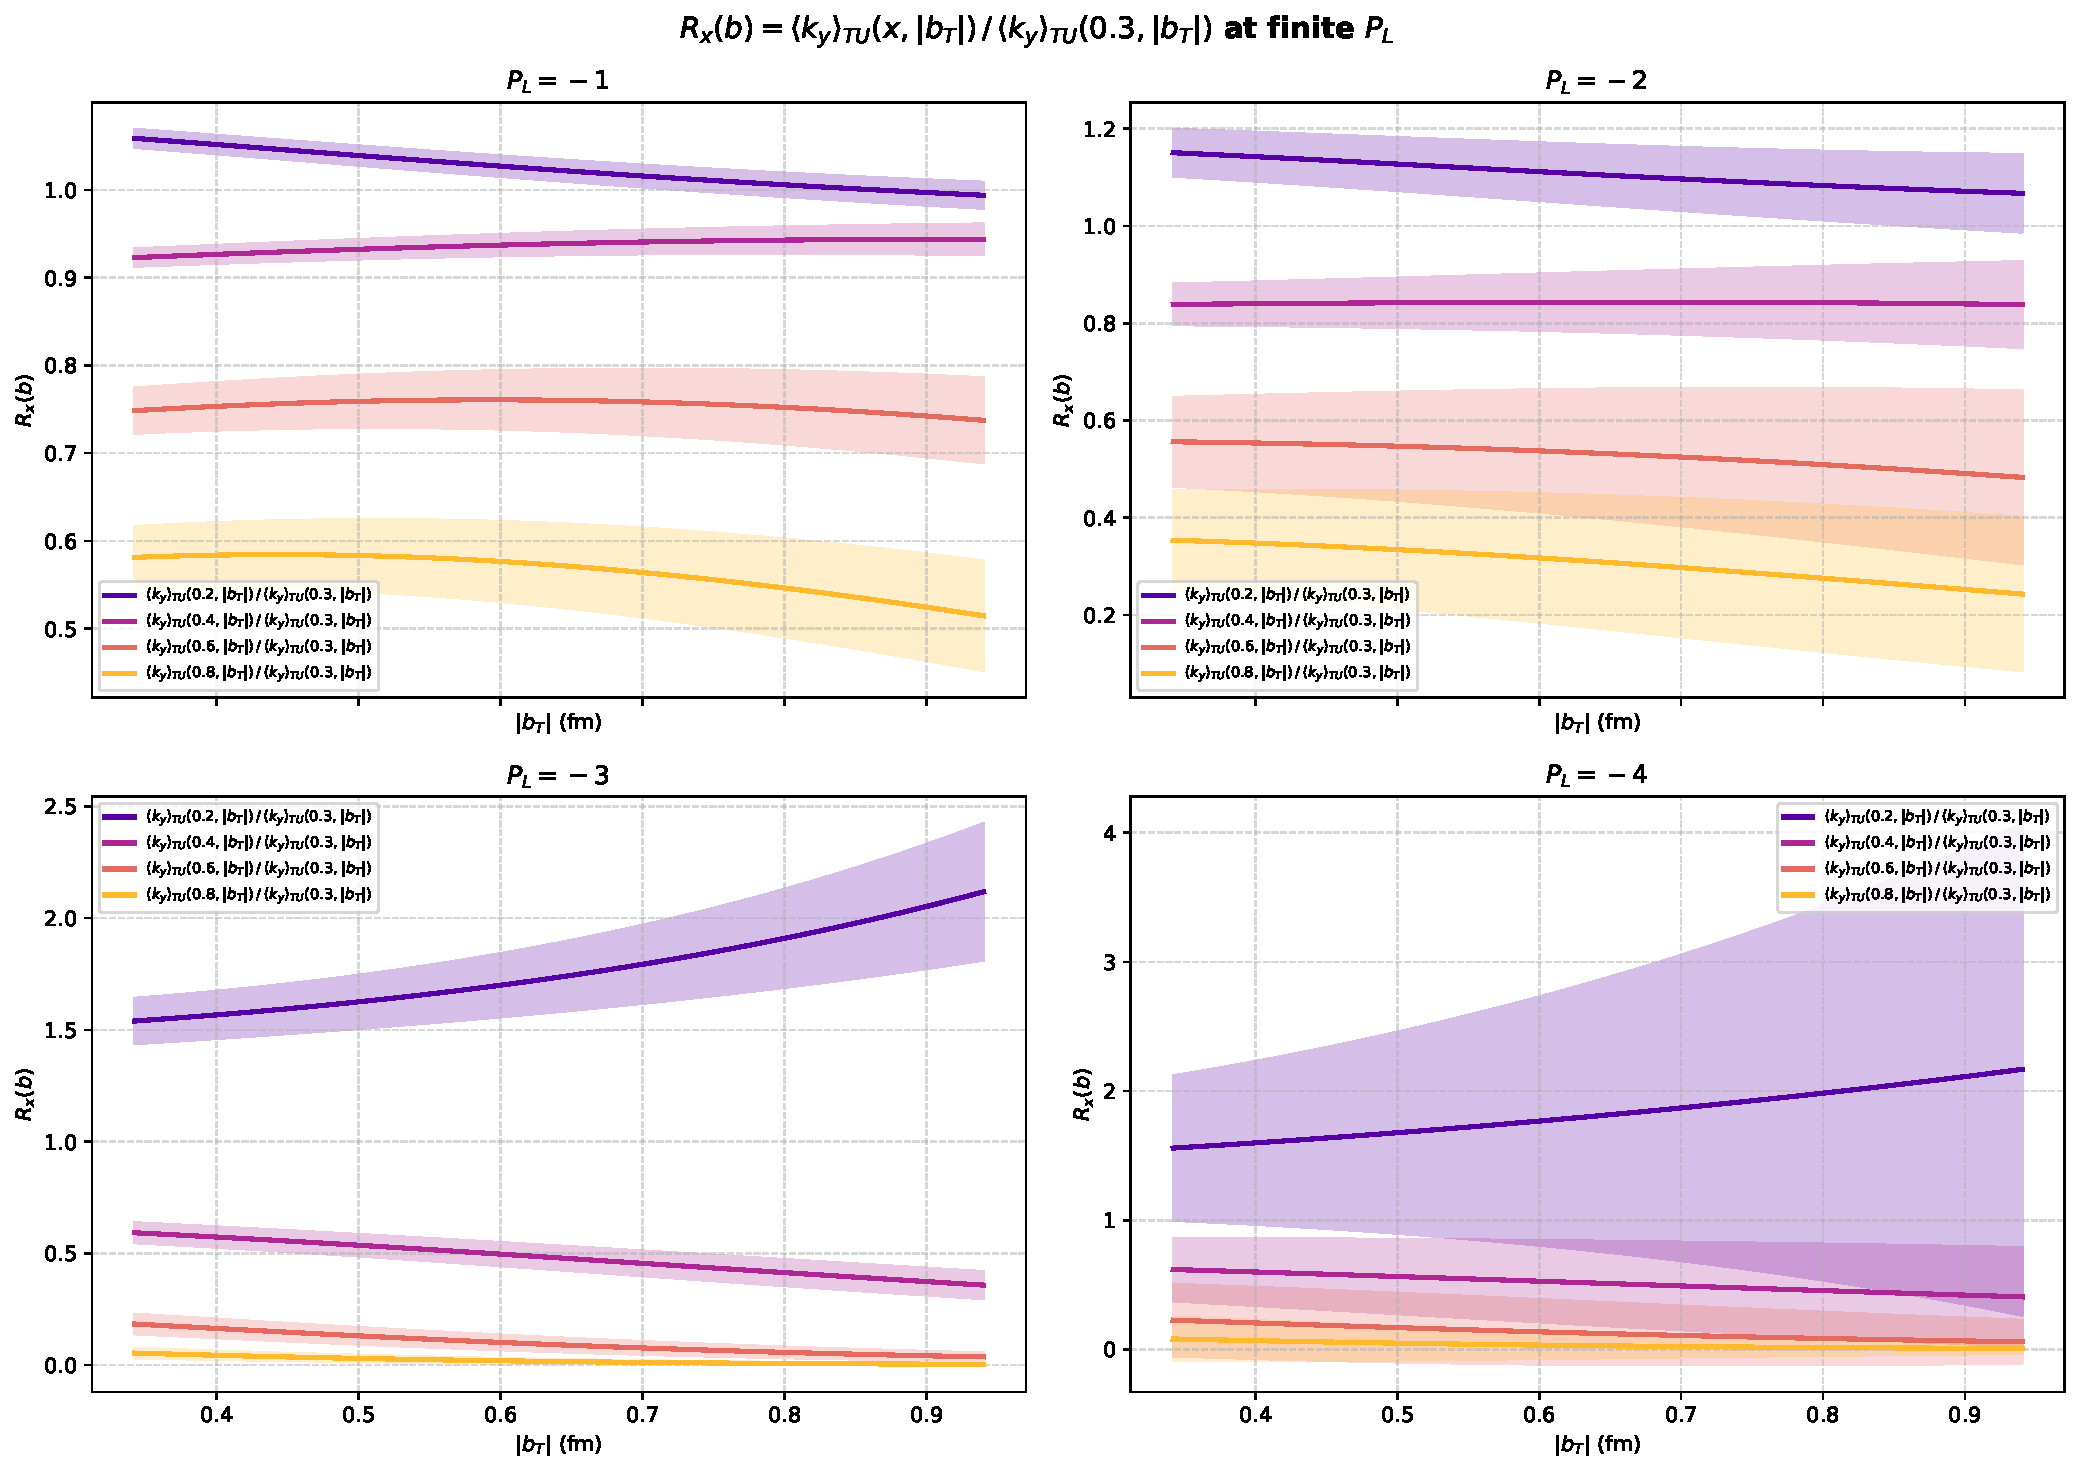
\includegraphics[width=\linewidth]{SimultaneousFitsCov/factorization_test/Factorization_Ratio_vs_bT_AllPL_bmin3_eta610.pdf}
    \caption{The same ratio test as Fig.~\ref{fig:factorization_ratio_bT_sivers}, $R_x(|b_T|)$, repeated at each finite momentum individually. The departure from flatness grows with $|P_L|$, most visibly in the $x=0.2$ curve, which is consistent with the parameter mismatch identified in the extrapolated $j_X$ and $d_X$ values above.}
    \label{fig:factorization_ratio_bT_finitePL}
\end{figure}

\subsubsection{Factorization Test at the Amplitude Level}
\label{sec:factorization_amplitude_test}

The Sivers-shift test above probes factorization of the full ratio $\langle k_y \rangle_{TU} = -m_N \tAmp_{12B}^{\text{Re}}/(\tAmp_{2B}^{\text{Re}} - i\tAmp_{2B}^{\text{Im}})$, in which some of the non-factorized behavior of the individual amplitudes could in principle cancel. We therefore repeat the identical distance test of Section~\ref{sec:factorization_metric} on each extrapolated amplitude separately: $\tAmp_{12B}^{\text{Re}}$, $\tAmp_{2B}^{\text{Re}}$, $i\tAmp_{2B}^{\text{Im}}$, and the combination $\tAmp_{2B}^{\text{Re}} - i\tAmp_{2B}^{\text{Im}}$ (proportional to $\tilde f_1^{[1](0)}$) that appears in the Sivers-shift denominator. Table~\ref{tab:factorization_amplitudes} lists the resulting relative distances, using the same $|b_T|\in[0.3421,0.9403]$ fm grid and four $x$-windows as the Sivers-shift test.

\begin{table}[h!]
    \centering
    \renewcommand{\arraystretch}{1.4}
    \caption{Relative distance of each extrapolated amplitude (and their combination $\tAmp_{2B}^{\text{Re}}-i\tAmp_{2B}^{\text{Im}}$) from its optimal factorized approximation, over the same $|b_T|\in[0.3421,0.9403]$ fm grid and $x$-windows as Table~\ref{tab:factorization_sivers}.}
    \label{tab:factorization_amplitudes}
    \begin{tabular}{|l|c|c|c|c|}
    \hline
    Amplitude & $x\in[0.0,1.0]$ & $x\in[0.1,0.9]$ & $x\in[0.2,0.8]$ & $x\in[0.3,0.8]$ \\
    \hline
    $\tAmp_{12B}^{\text{Re}}$ & $0.0804(18)$ & $0.0573(26)$ & $0.0397(24)$ & $0.0303(21)$ \\
    \hline
    $\tAmp_{2B}^{\text{Re}}$ & $0.08138(65)$ & $0.0718(36)$ & $0.0581(55)$ & $0.0478(56)$ \\
    \hline
    $i\tAmp_{2B}^{\text{Im}}$ & $0.107(18)$ & $0.0868(30)$ & $0.0578(28)$ & $0.0425(23)$ \\
    \hline
    $\tAmp_{2B}^{\text{Re}} - i\tAmp_{2B}^{\text{Im}}$ & $0.1943(63)$ & $0.0926(59)$ & $0.0594(40)$ & $0.0470(47)$ \\
    \hline
    \end{tabular}
\end{table}

Every individual amplitude shows a nonzero relative distance from factorized form in every window, and for the widest window, $x\in[0,1]$, the amplitude-level residuals ($8$-$19\%$) are larger than the corresponding Sivers-ratio residual ($5.7\%$ from Table~\ref{tab:factorization_sivers}): the ratio structure of the Sivers shift partially, but not completely, cancels the non-factorized behavior present in the individual amplitudes. All four amplitude-level residuals shrink as the $x$-window is narrowed away from $x=0$, consistent with each amplitude's own Bessel-function singularity structure near the origin, which differs amplitude by amplitude because of the parameter mismatch identified in Section~\ref{sec:factorization_sivers_test}.

\begin{figure}[h!]
    \centering
    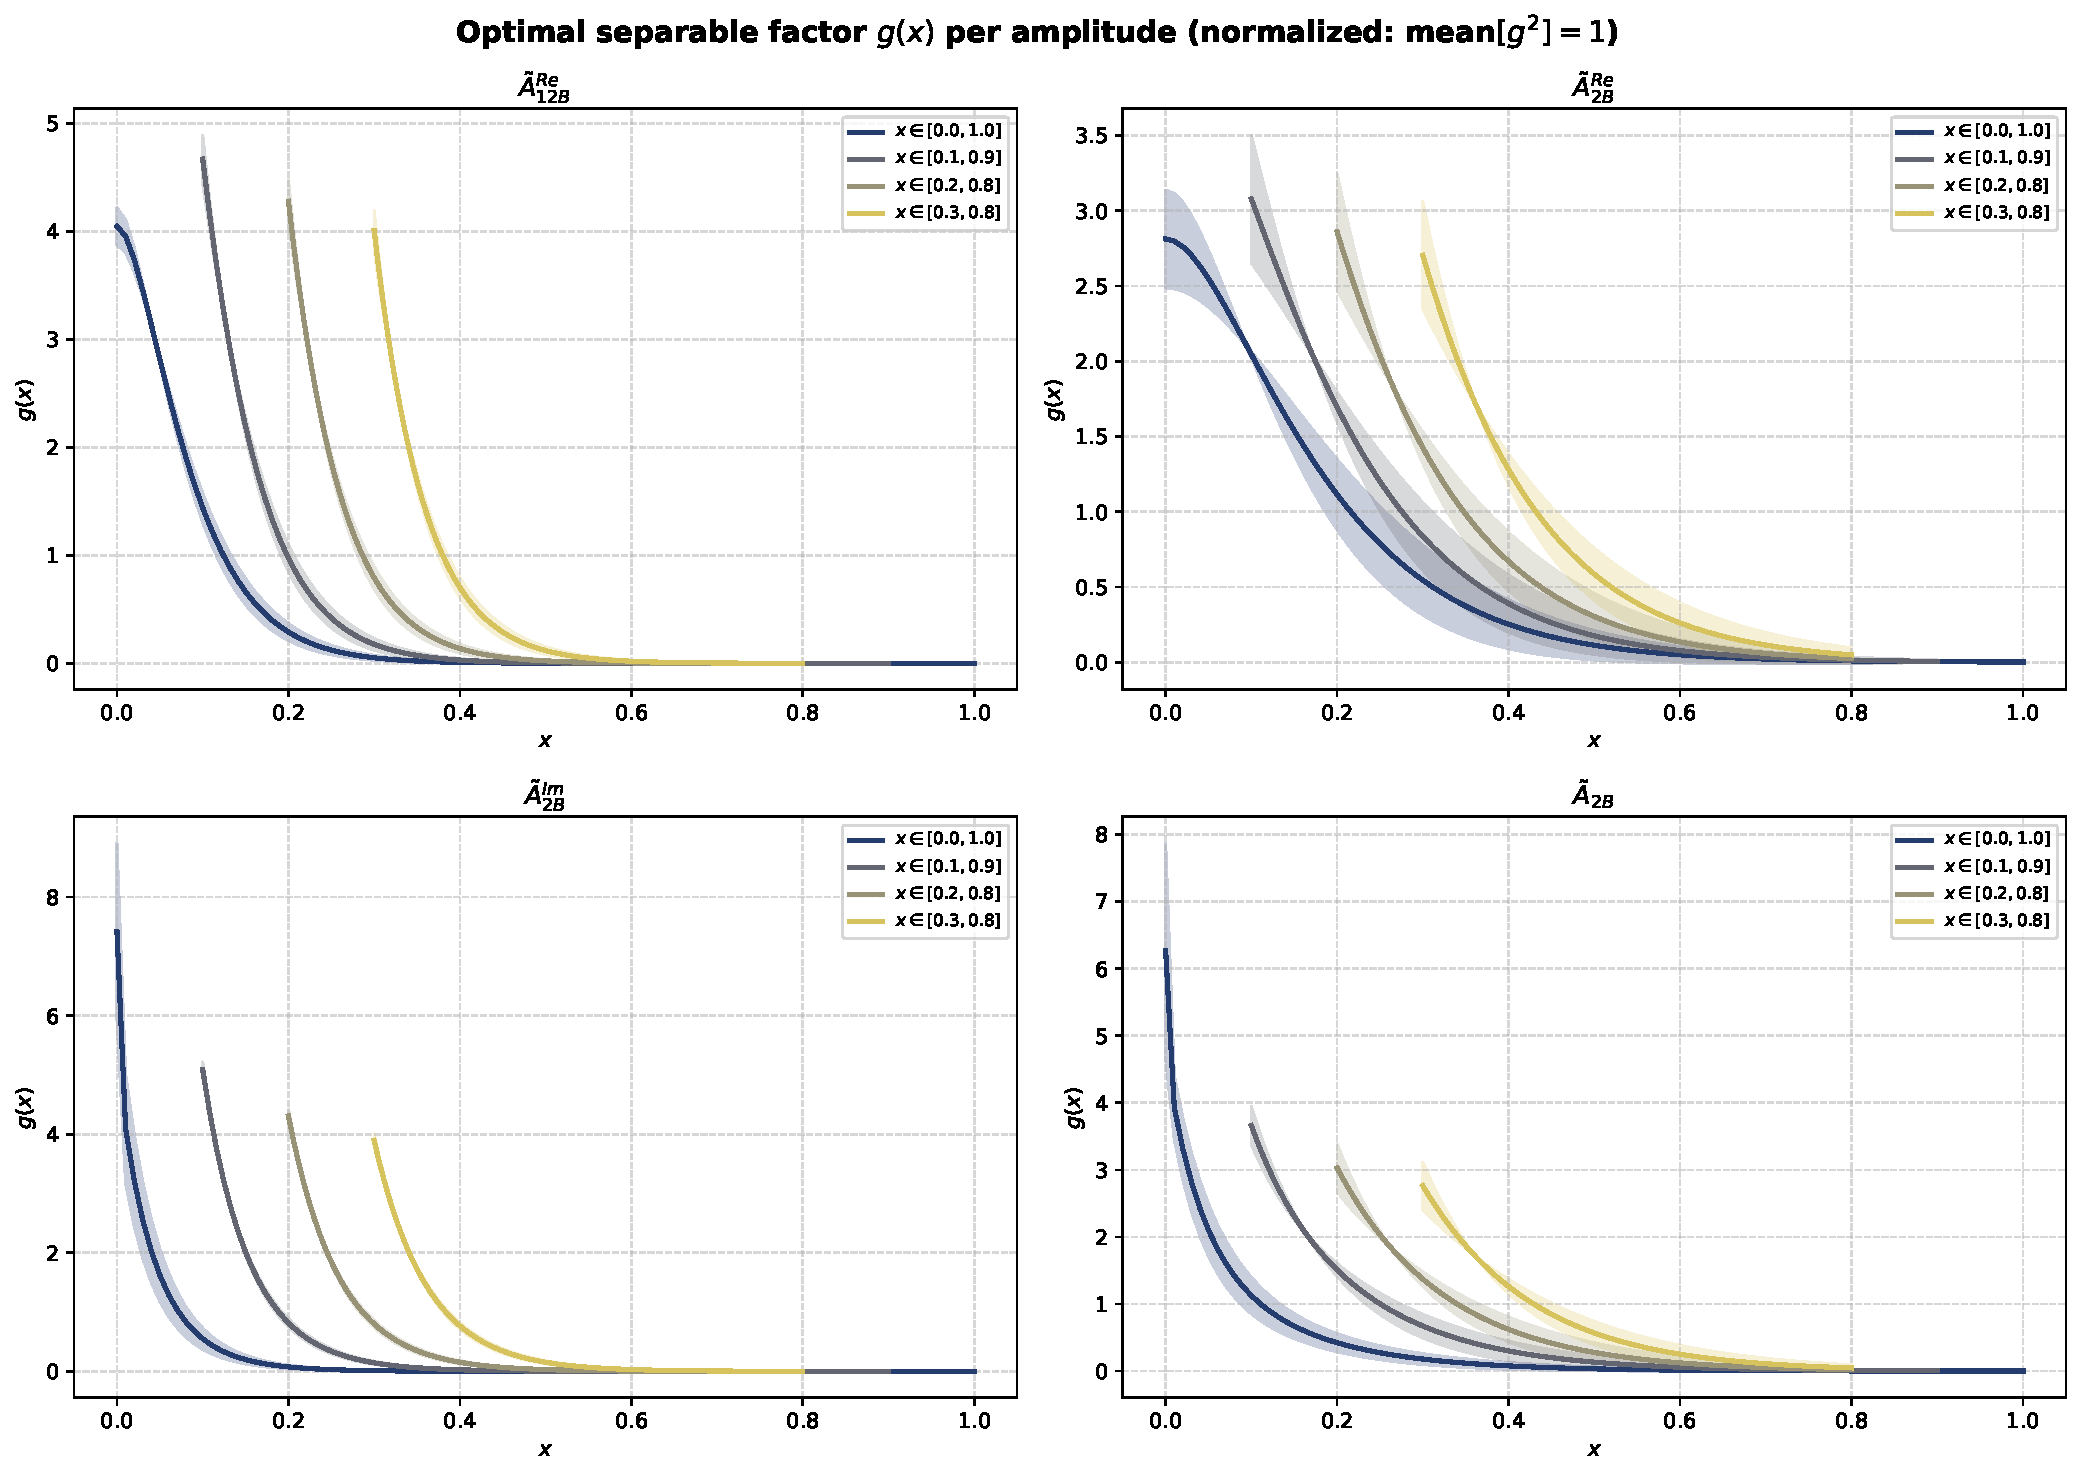
\includegraphics[width=\linewidth]{SimultaneousFitsCov/factorization_test/Factorization_Amplitudes_g_of_x_bmin3_eta610.pdf}
    \caption{Optimal separable factor $g(x)$ for each of the four amplitude combinations of Table~\ref{tab:factorization_amplitudes}, for all four $x$-windows (normalized so $\text{mean}[g^2]=1$). Each amplitude's $g(x)$ is dominated by a sharp rise as $x\to0$ that steepens as the window narrows, reflecting the Bessel-function behavior at small $x$.}
    \label{fig:factorization_g_amplitudes}
\end{figure}

\begin{figure}[h!]
    \centering
    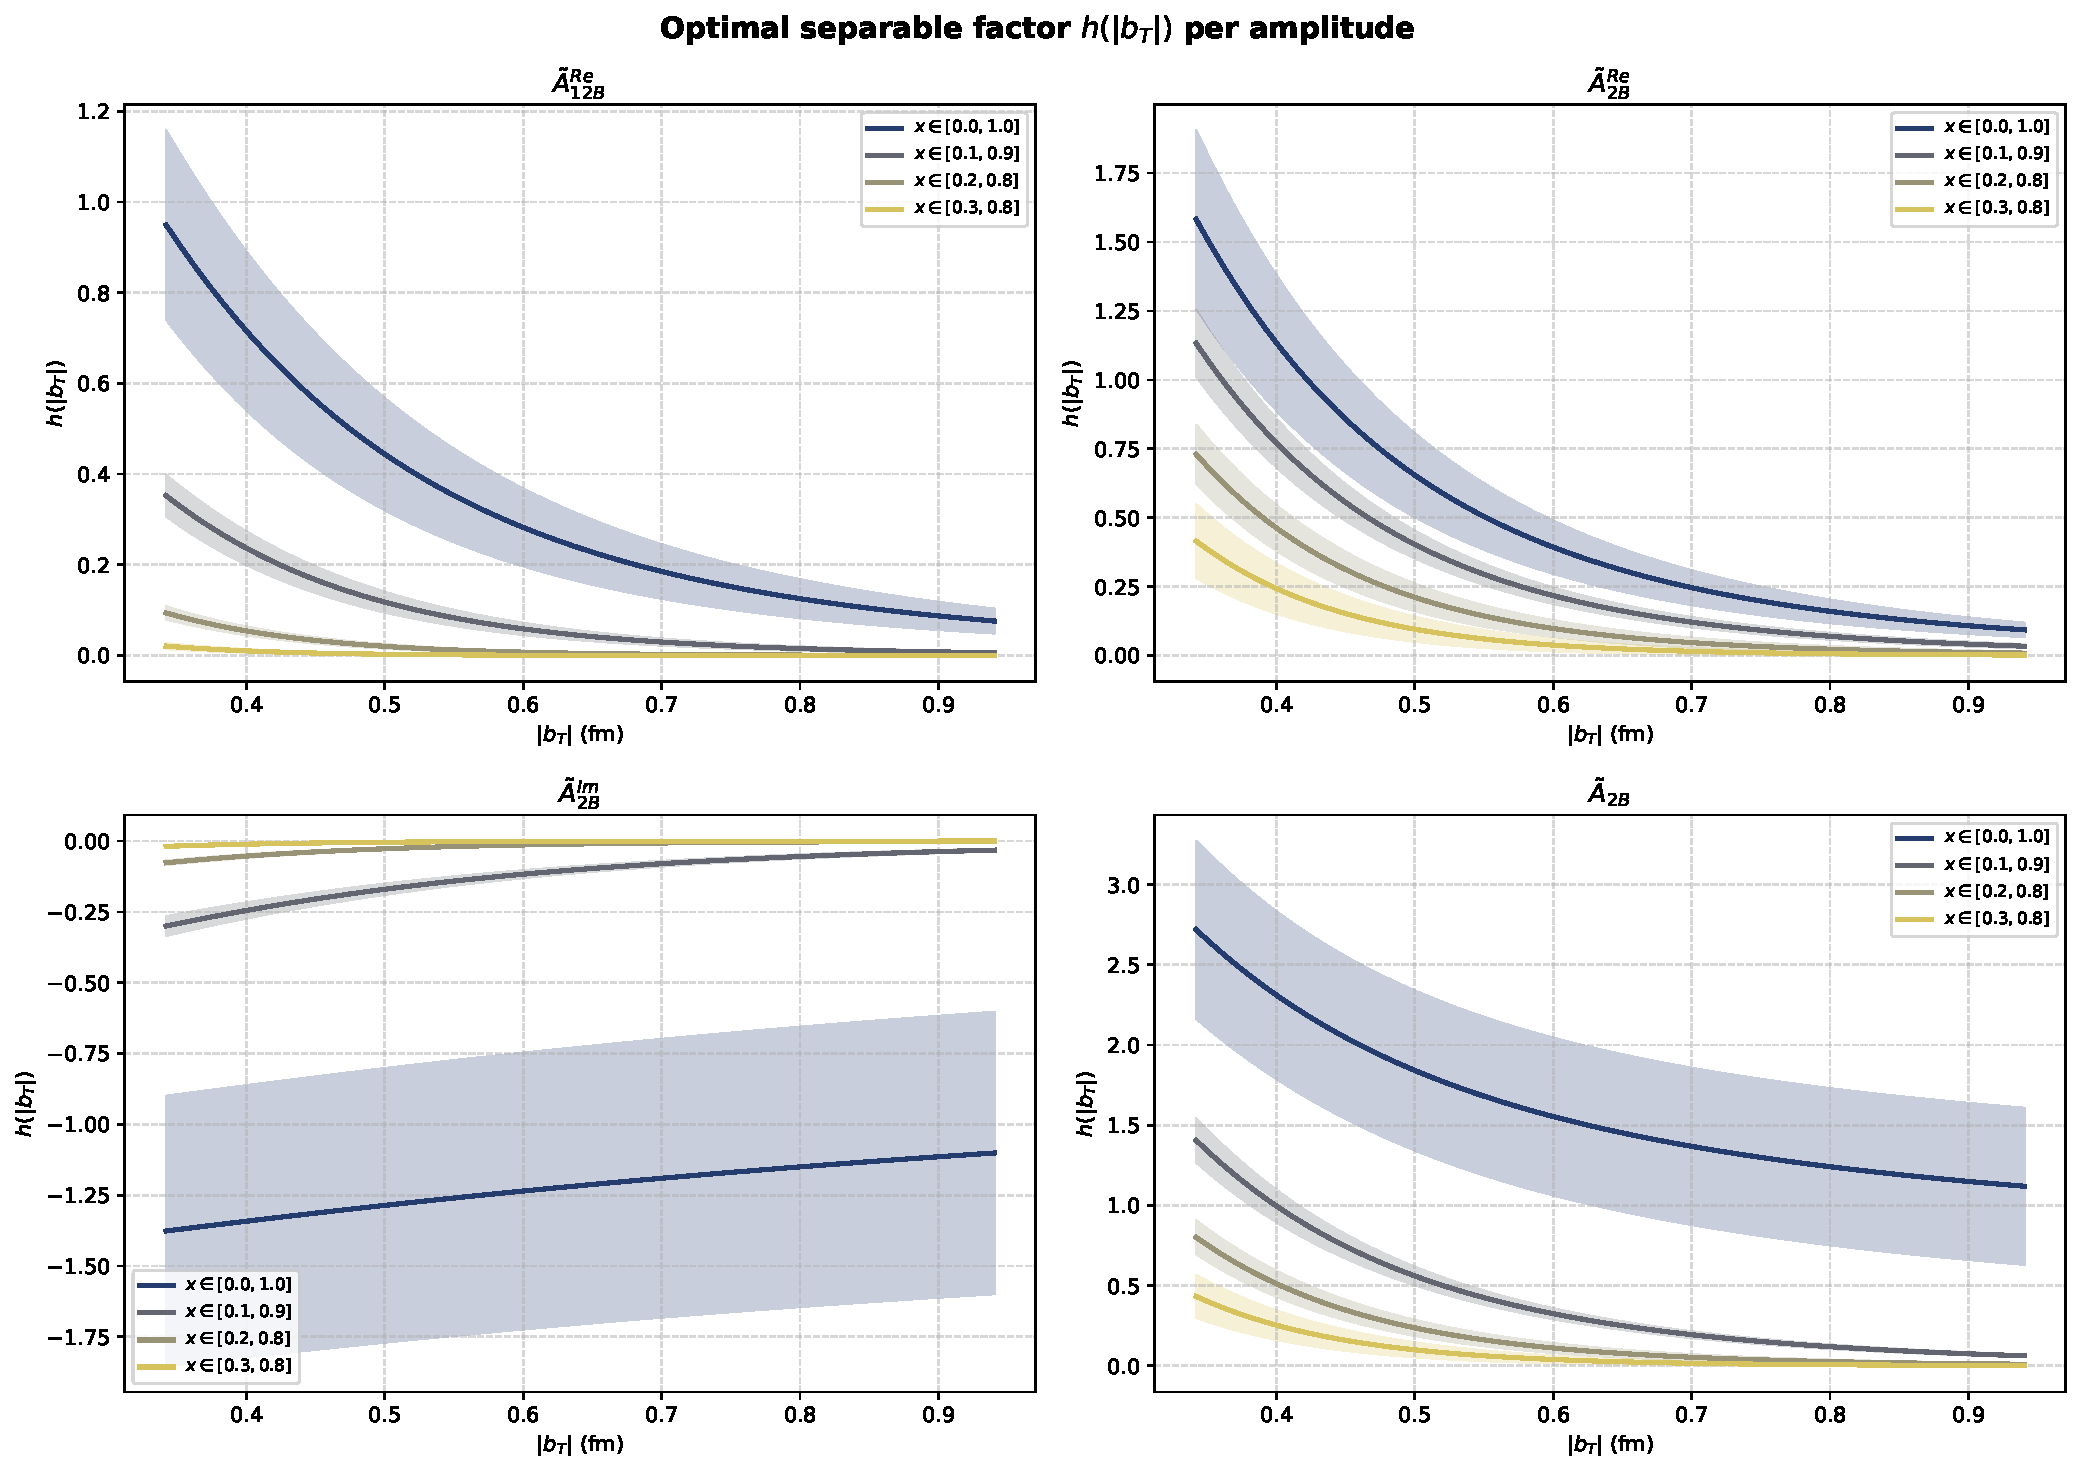
\includegraphics[width=\linewidth]{SimultaneousFitsCov/factorization_test/Factorization_Amplitudes_h_of_bT_bmin3_eta610.pdf}
    \caption{Optimal separable factor $h(|b_T|)$ for each of the four amplitude combinations of Table~\ref{tab:factorization_amplitudes}, for all four $x$-windows. All four amplitudes' $h(|b_T|)$ fall smoothly with increasing $|b_T|$, but with a magnitude and slope that depends on the $x$-window used to define the fit, itself a signature of imperfect factorization.}
    \label{fig:factorization_h_amplitudes}
\end{figure}

\begin{figure}[h!]
    \centering
    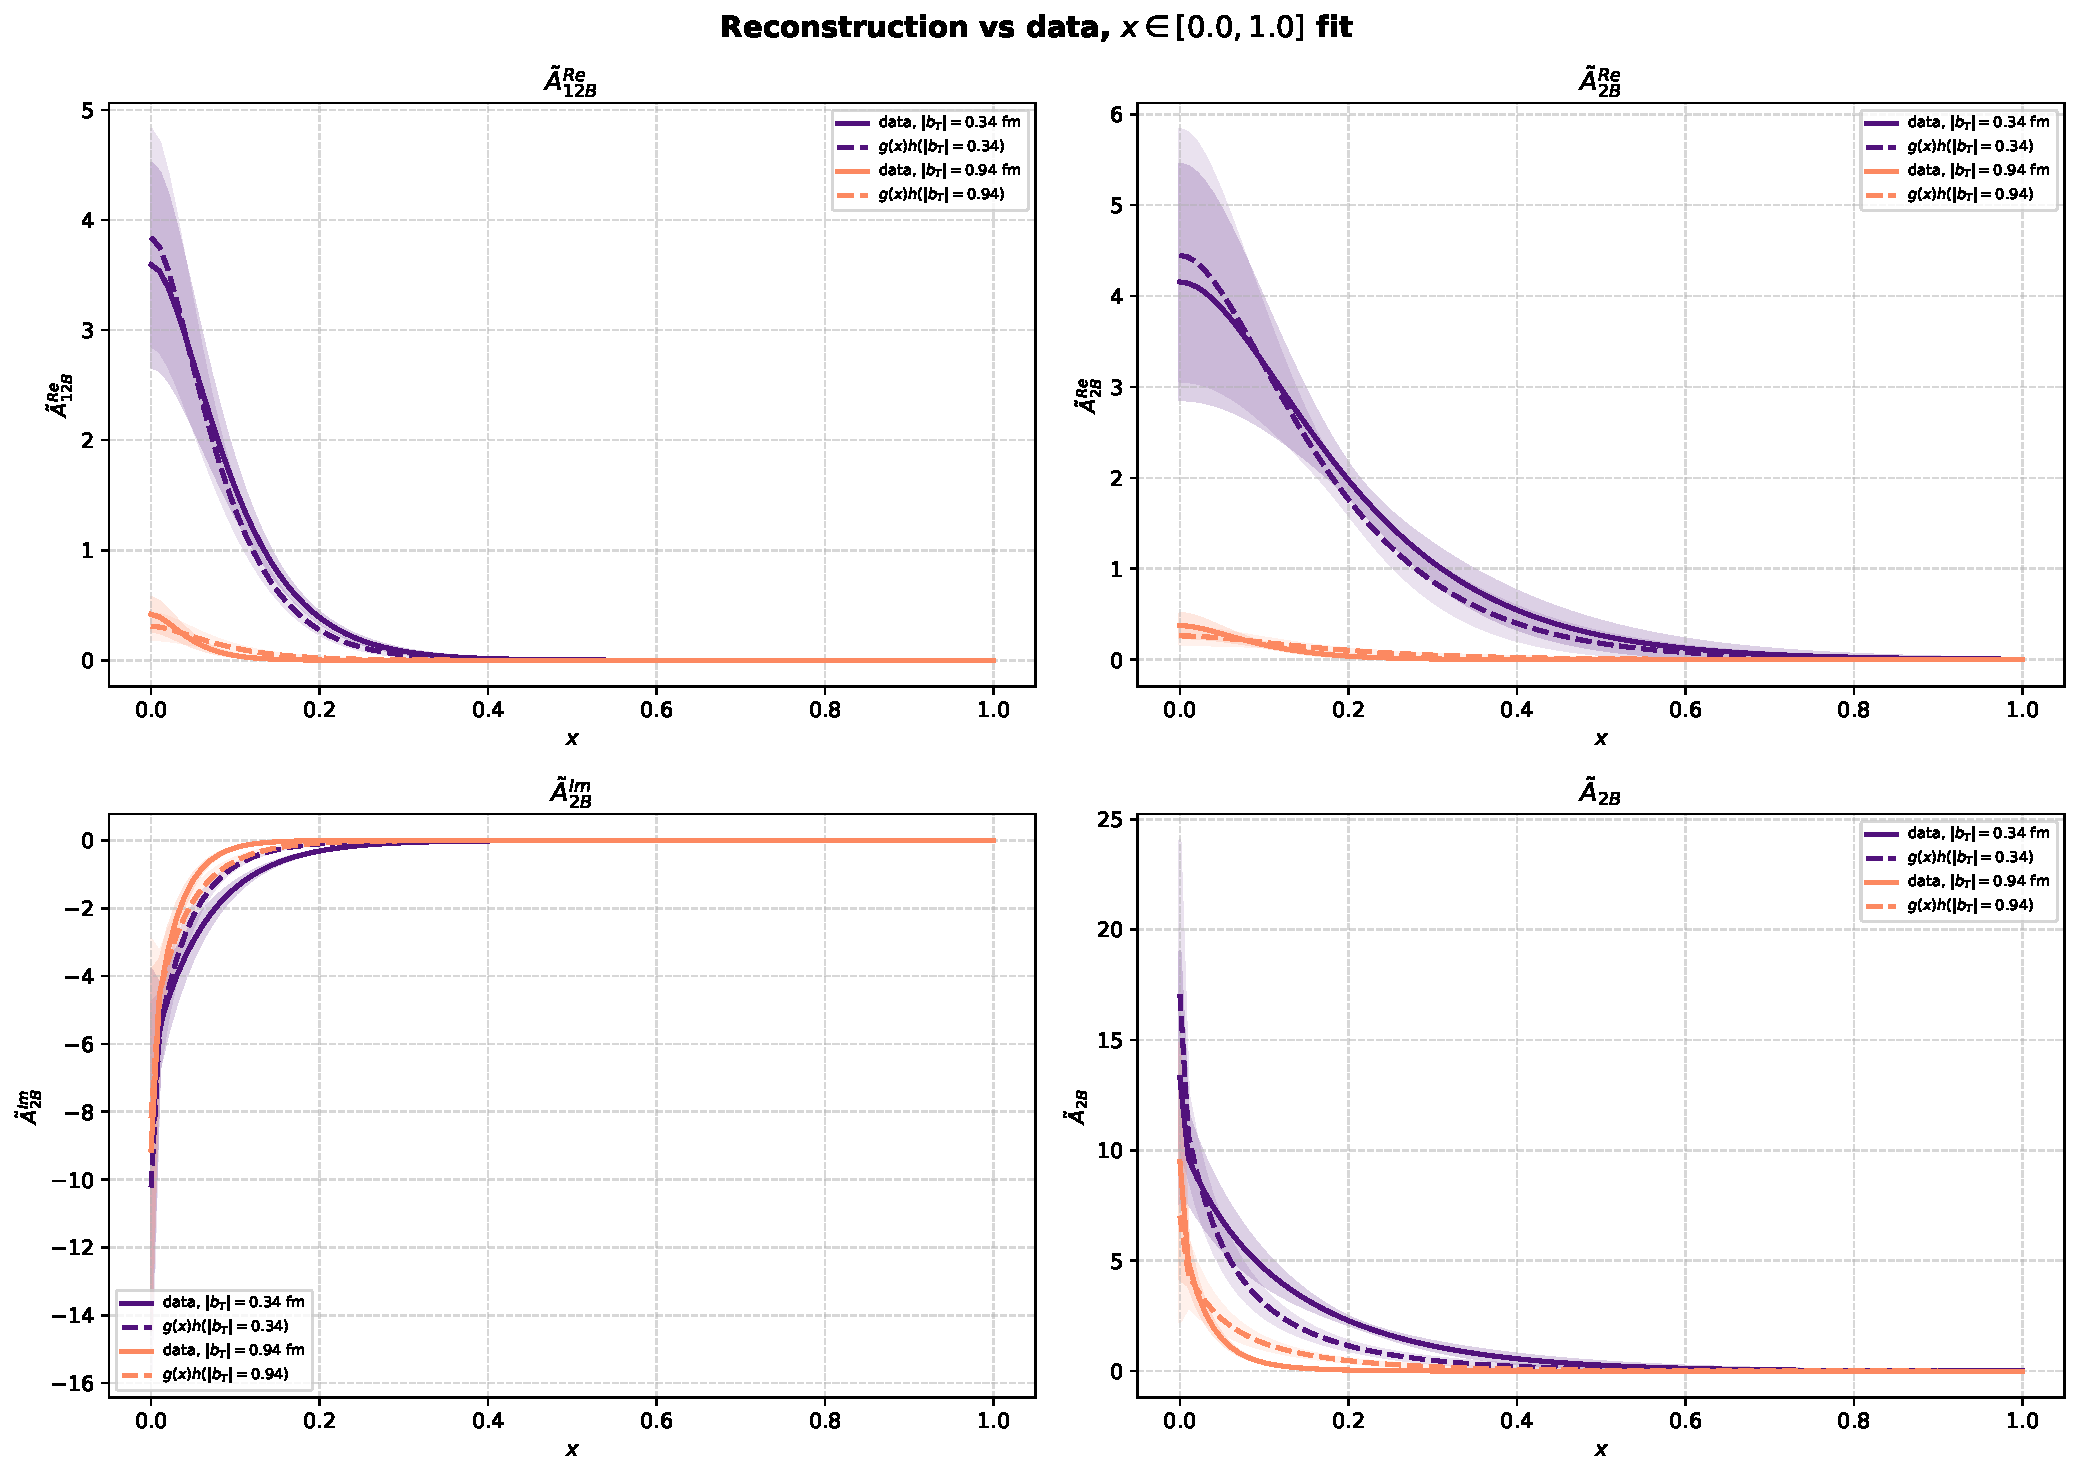
\includegraphics[width=\linewidth]{SimultaneousFitsCov/factorization_test/Factorization_Amplitudes_Reconstruction_bmin3_eta610.pdf}
    \caption{Reconstructed $g(x)h(|b_T|)$ (dashed) against the actual extrapolated amplitude data (solid) at the smallest and largest fitted $|b_T|$, using the $x\in[0,1]$ fit, for each of the four amplitude combinations of Table~\ref{tab:factorization_amplitudes}. The largest reconstruction gap appears near $x\to0$ for every amplitude, matching the $x\in[0,1]$ column of Table~\ref{tab:factorization_amplitudes} being the largest relative distance in every row.}
    \label{fig:factorization_reconstruction_amplitudes}
\end{figure}

Taken together, the Sivers-shift and amplitude-level tests give a consistent picture: neither the individual amplitudes nor the Sivers-shift ratio built from them are exactly factorized in $x$ and $|b_T|$, but the deviation from a factorized form is a modest, well-resolved residual rather than a qualitative failure. The Sivers shift itself is factorized to within roughly $6$-$8\%$ in the relative $L_2$ sense, smaller than the $8$-$19\%$ residuals of the amplitudes that enter it, indicating a partial cancellation of non-factorized behavior in the ratio. This residual is traced directly to the extrapolated fit parameters: the Bessel-function order $j_{\text{im}}\approx1$ governing $\tAmp_{2B}^{\text{Im}}$ differs from $j_{\text{re}},j_{\text{reA12B}}\approx2$ governing the two real amplitudes, and the three width parameters $d_X$ are likewise resolved from one another well outside their Jackknife uncertainties. We conclude that an exactly factorized ansatz $F(x)G(|b_T|)$ would be a good, but not exact, approximation to the extracted Sivers shift.

\newpage
~
\newpage
~
\newpage
\input{Chapters/CONCLUSION}
\newpage
\appendix
\section{QLUA: Gamma $\Gamma(n)$}
The binary notation for 16 basis matrices:
\begin{align}
    \Gamma(n)=\gamma_{1}^{n_{0}}\gamma_{2}^{n_{1}}\gamma_{3}^{n_{2}}\gamma_{4}^{n_{3}}
\end{align}
where, the binary representation of $[n]_{10}$ is $[n_{3}n_{2}n_{1}n_{0}]_{2}$
\begin{align}
    [n]_{10}=n_{3}2^{3}+n_{2}2^{2}+n_{1}2^{1}+n_{0}2^{0}
\end{align}
The below table contains all 16 gamma matrices with binary notations.
\begin{table}[h!]
\centering
\scalebox{1.4}{
\begin{tabular}{|c|c||c|}
\hline
  $[n]_{10}$    & $[n_{3}n_{2}n_{1}n_{0}]_{2}$ & $\Gamma(n)$ \\
  \hline
  \hline
    $0$ & $0000$ & $\mathbbm{1}$\\
   \hline
    $1$ & $0001$ & $\gamma_{1}$\\
   \hline
    $2$ & $0010$ & $\gamma_{2}$\\
   \hline
    $3$ & $0011$ & $\gamma_{1}\gamma_{2}$\\
   \hline
    $4$ & $0100$ & $\gamma_{3}$\\
   \hline
    $5$ & $0101$ & $\gamma_{1}\gamma_{3}$\\
   \hline
    $6$ & $0110$ & $\gamma_{2}\gamma_{3}$\\
   \hline
    $7$ & $0111$ & $\gamma_{1}\gamma_{2}\gamma_{3}$=$\gamma_{5}\gamma_{4}$\\
   \hline
    $8$ & $1000$ & $\gamma_{4}$\\
   \hline
    $9$ & $1001$ & $\gamma_{1}\gamma_{4}$\\
   \hline
    $10$ & $1010$ & $\gamma_{2}\gamma_{4}$\\
   \hline
    $11$ & $1011$ & $\gamma_{1}\gamma_{2}\gamma_{4}=-\gamma_{5}\gamma_{3}$\\
   \hline
    $12$ & $1100$ & $\gamma_{3}\gamma_{4}$\\
   \hline
    $13$ & $1101$ & $\gamma_{1}\gamma_{3}\gamma_{4}=\gamma_{5}\gamma_{2}$\\
   \hline
    $14$ & $1110$ & $\gamma_{2}\gamma_{3}\gamma_{4}=-\gamma_{5}\gamma_{1}$\\
   \hline
    $15$ & $1111$ & $\gamma_{1}\gamma_{2}\gamma_{3}\gamma_{4}=\gamma_{5}$\\
   \hline
\end{tabular}}
\end{table}

\clearpage
\section{Extended Global Simultaneous Fits for Higher Momenta}
\label{app:higher_momenta_fits}

This appendix provides the detailed multi-dimensional fit surfaces and Jackknife covariance matrices for the global simultaneous fits performed at higher simulated nucleon momenta $P_L \in \{-2, -3, -4\}$. As discussed in Section \ref{sec:simultaneous_fit}, these extensive diagnostic plots demonstrate the structural consistency and stability of the extracted parameters across all evaluated momenta, mirroring the baseline $P_L = -1$ results.

\renewcommand{\PLval}{-2}
\subsection{\texorpdfstring{Diagnostic Plots for $\vect{P}\cdot a\hat{L}/(2\pi)=\{\PLval,0,0\}$}{TEXT}}
\begin{figure}[htbp]
    \centering
    \begin{tabular}{ccc}
        % Column Headers
        \textbf{$\widetilde{A}^{Re}_{2B}$} & \textbf{$\widetilde{A}^{Im}_{2B}$} & \textbf{$\widetilde{A}^{Re}_{12B}$} \\[2ex]
        \includegraphics[width=0.3\linewidth]{plots/Amps_Fit/ReA12B_Pb_bsq_PL\PLval_WithFit_3D.pdf} &
        \includegraphics[width=0.3\linewidth]{plots/Amps_Fit/ImA2B_PL\PLval_WithFit_3D.pdf} &
        \includegraphics[width=0.3\linewidth]{plots/Amps_Fit/ReA12B_PL\PLval_WithFit_3D.pdf}\\[2ex]
        \includegraphics[width=0.3\linewidth]{plots/Amps_Fit/ReA2B_Pb_bsq_PL\PLval_WithFit_3D.pdf} &
        \includegraphics[width=0.3\linewidth]{plots/Amps_Fit/ImA2B_Pb_bsq_PL\PLval_WithFit_3D.pdf} &
        \includegraphics[width=0.3\linewidth]{plots/Amps_Fit/ReA12B_Pb_bsq_PL\PLval_WithFit_3D.pdf} \\
    \end{tabular}
    \caption{Fit for $\widetilde{A}^{Re}_{2B}$, $\widetilde{A}^{Im}_{2B}$ \& $\widetilde{A}^{Re}_{12B}$ amplitudes for $\vect{P}\cdot a\hat{L}/(2\pi)=\{\PLval,0,0\}$. The top row displays the $(b_{L}/a,b_{T}/a,\eta|\vect{v}|/a)-$space, while the bottom row displays the $((\vect{P}\cdot \vect{b})\cdot\hat{L}/(2\pi),b^{2}/a^2,\eta|\vect{v}|/a)-$space with the global simultaneous fit overlaid.}
    \label{fig:A2B_amplitudes_fit_P2}
\end{figure}

\begin{figure}[htbp]
    \centering
    \begin{tabular}{c}
        \includegraphics[width=0.9\linewidth]{plots/Amps_Fit/Combined_eta8_PL\PLval_WithFit_2D.pdf} \\
        \includegraphics[width=0.9\linewidth]{plots/Amps_Fit/Combined_Pb_bsq_eta8_PL\PLval_WithFit_2D.pdf} \\
    \end{tabular}
    \caption{Fit for $\widetilde{A}^{Re}_{2B}$, $\widetilde{A}^{Im}_{2B}$ \& $\widetilde{A}^{Re}_{12B}$ amplitudes for $\vect{P}\cdot a\hat{L}/(2\pi)=\{\PLval,0,0\}$ at a fixed staple extent $\eta|\vect{v}|/a=8$. The top two rows display the $(b_{L}/a,b_{T}/a)-$space, while the bottom two rows display the $((\vect{P}\cdot \vect{b})\cdot\hat{L}/(2\pi),b^{2}/a^2)-$space with the fit.}
    \label{fig:combined_fit_P2}
\end{figure}

\begin{figure}[htbp]
    \centering
    \includegraphics[width=0.5\linewidth]{SimultaneousFitsCov/SimulFitCovMatrix-A12B-A2B-FT-a_im-a_re-a_reA12B-c_im-c_re-c_reA12B-d_im-d_re-d_reA12B-f-j_im-j_re-j_reA12B-k1_re-k2_re__bmin3_eta610_PL\PLval.pdf}
    \caption{2D representation of the full Jackknife covariance matrix utilized in the simultaneous fit for $P_L=-2$.}
    \label{fig:cov_matrix_2d_P2}
\end{figure}

\begin{figure}[htbp]
    \centering
    \includegraphics[width=0.7\linewidth]{SimultaneousFitsCov/SimulFitCovMatrix-A12B-A2B-FT-3D_a_im-a_re-a_reA12B-c_im-c_re-c_reA12B-d_im-d_re-d_reA12B-f-j_im-j_re-j_reA12B-k1_re-k2_re__bmin3_eta610_PL\PLval.pdf}
    \caption{3D surface plot of the Jackknife covariance matrix for $P_L=-2$.}
    \label{fig:cov_matrix_3d_P2}
\end{figure}

\clearpage
\renewcommand{\PLval}{-3}
\subsection{\texorpdfstring{Diagnostic Plots for $\vect{P}\cdot a\hat{L}/(2\pi)=\{\PLval,0,0\}$}{TEXT}}
\begin{figure}[htbp]
    \centering
    \begin{tabular}{ccc}
        % Column Headers
        \textbf{$\widetilde{A}^{Re}_{2B}$} & \textbf{$\widetilde{A}^{Im}_{2B}$} & \textbf{$\widetilde{A}^{Re}_{12B}$} \\[2ex]
        \includegraphics[width=0.3\linewidth]{plots/Amps_Fit/ReA12B_Pb_bsq_PL\PLval_WithFit_3D.pdf} &
        \includegraphics[width=0.3\linewidth]{plots/Amps_Fit/ImA2B_PL\PLval_WithFit_3D.pdf} &
        \includegraphics[width=0.3\linewidth]{plots/Amps_Fit/ReA12B_PL\PLval_WithFit_3D.pdf}\\[2ex]
        \includegraphics[width=0.3\linewidth]{plots/Amps_Fit/ReA2B_Pb_bsq_PL\PLval_WithFit_3D.pdf} &
        \includegraphics[width=0.3\linewidth]{plots/Amps_Fit/ImA2B_Pb_bsq_PL\PLval_WithFit_3D.pdf} &
        \includegraphics[width=0.3\linewidth]{plots/Amps_Fit/ReA12B_Pb_bsq_PL\PLval_WithFit_3D.pdf} \\
    \end{tabular}
    \caption{Fit for $\widetilde{A}^{Re}_{2B}$, $\widetilde{A}^{Im}_{2B}$ \& $\widetilde{A}^{Re}_{12B}$ amplitudes for $\vect{P}\cdot a\hat{L}/(2\pi)=\{\PLval,0,0\}$. The top row displays the $(b_{L}/a,b_{T}/a,\eta|\vect{v}|/a)-$space, while the bottom row displays the $((\vect{P}\cdot \vect{b})\cdot\hat{L}/(2\pi),b^{2}/a^2,\eta|\vect{v}|/a)-$space with the global simultaneous fit overlaid.}
    \label{fig:A2B_amplitudes_fit_P3}
\end{figure}

\begin{figure}[htbp]
    \centering
    \begin{tabular}{c}
        \includegraphics[width=0.9\linewidth]{plots/Amps_Fit/Combined_eta8_PL\PLval_WithFit_2D.pdf} \\
        \includegraphics[width=0.9\linewidth]{plots/Amps_Fit/Combined_Pb_bsq_eta8_PL\PLval_WithFit_2D.pdf} \\
    \end{tabular}
    \caption{Fit for $\widetilde{A}^{Re}_{2B}$, $\widetilde{A}^{Im}_{2B}$ \& $\widetilde{A}^{Re}_{12B}$ amplitudes for $\vect{P}\cdot a\hat{L}/(2\pi)=\{\PLval,0,0\}$ at a fixed staple extent $\eta|\vect{v}|/a=8$. The top two rows display the $(b_{L}/a,b_{T}/a)-$space, while the bottom two rows display the $((\vect{P}\cdot \vect{b})\cdot\hat{L}/(2\pi),b^{2}/a^2)-$space with the fit.}
    \label{fig:combined_fit_P3}
\end{figure}

\begin{figure}[htbp]
    \centering
    \includegraphics[width=0.5\linewidth]{SimultaneousFitsCov/SimulFitCovMatrix-A12B-A2B-FT-a_im-a_re-a_reA12B-c_im-c_re-c_reA12B-d_im-d_re-d_reA12B-f-j_im-j_re-j_reA12B-k1_re-k2_re__bmin3_eta610_PL\PLval.pdf}
    \caption{2D representation of the full Jackknife covariance matrix utilized in the simultaneous fit for $P_L=-3$.}
    \label{fig:cov_matrix_2d_P3}
\end{figure}

\begin{figure}[htbp]
    \centering
    \includegraphics[width=0.7\linewidth]{SimultaneousFitsCov/SimulFitCovMatrix-A12B-A2B-FT-3D_a_im-a_re-a_reA12B-c_im-c_re-c_reA12B-d_im-d_re-d_reA12B-f-j_im-j_re-j_reA12B-k1_re-k2_re__bmin3_eta610_PL\PLval.pdf}
    \caption{3D surface plot of the Jackknife covariance matrix for $P_L=-3$.}
    \label{fig:cov_matrix_3d_P3}
\end{figure}

\clearpage
\renewcommand{\PLval}{-4}
\subsection{\texorpdfstring{Diagnostic Plots for $\vect{P}\cdot a\hat{L}/(2\pi)=\{\PLval,0,0\}$}{TEXT}}
\begin{figure}[htbp]
    \centering
    \begin{tabular}{ccc}
        % Column Headers
        \textbf{$\widetilde{A}^{Re}_{2B}$} & \textbf{$\widetilde{A}^{Im}_{2B}$} & \textbf{$\widetilde{A}^{Re}_{12B}$} \\[2ex]
        \includegraphics[width=0.3\linewidth]{plots/Amps_Fit/ReA12B_Pb_bsq_PL\PLval_WithFit_3D.pdf} &
        \includegraphics[width=0.3\linewidth]{plots/Amps_Fit/ImA2B_PL\PLval_WithFit_3D.pdf} &
        \includegraphics[width=0.3\linewidth]{plots/Amps_Fit/ReA12B_PL\PLval_WithFit_3D.pdf}\\[2ex]
        \includegraphics[width=0.3\linewidth]{plots/Amps_Fit/ReA2B_Pb_bsq_PL\PLval_WithFit_3D.pdf} &
        \includegraphics[width=0.3\linewidth]{plots/Amps_Fit/ImA2B_Pb_bsq_PL\PLval_WithFit_3D.pdf} &
        \includegraphics[width=0.3\linewidth]{plots/Amps_Fit/ReA12B_Pb_bsq_PL\PLval_WithFit_3D.pdf} \\
    \end{tabular}
    \caption{Fit for $\widetilde{A}^{Re}_{2B}$, $\widetilde{A}^{Im}_{2B}$ \& $\widetilde{A}^{Re}_{12B}$ amplitudes for $\vect{P}\cdot a\hat{L}/(2\pi)=\{\PLval,0,0\}$. The top row displays the $(b_{L}/a,b_{T}/a,\eta|\vect{v}|/a)-$space, while the bottom row displays the $((\vect{P}\cdot \vect{b})\cdot\hat{L}/(2\pi),b^{2}/a^2,\eta|\vect{v}|/a)-$space with the global simultaneous fit overlaid.}
    \label{fig:A2B_amplitudes_fit_P4}
\end{figure}

\begin{figure}[htbp]
    \centering
    \begin{tabular}{c}
        \includegraphics[width=0.9\linewidth]{plots/Amps_Fit/Combined_eta8_PL\PLval_WithFit_2D.pdf} \\
        \includegraphics[width=0.9\linewidth]{plots/Amps_Fit/Combined_Pb_bsq_eta8_PL\PLval_WithFit_2D.pdf} \\
    \end{tabular}
    \caption{Fit for $\widetilde{A}^{Re}_{2B}$, $\widetilde{A}^{Im}_{2B}$ \& $\widetilde{A}^{Re}_{12B}$ amplitudes for $\vect{P}\cdot a\hat{L}/(2\pi)=\{\PLval,0,0\}$ at a fixed staple extent $\eta|\vect{v}|/a=8$. The top two rows display the $(b_{L}/a,b_{T}/a)-$space, while the bottom two rows display the $((\vect{P}\cdot \vect{b})\cdot\hat{L}/(2\pi),b^{2}/a^2)-$space with the fit.}
    \label{fig:combined_fit_P4}
\end{figure}

\begin{figure}[htbp]
    \centering
    \includegraphics[width=0.5\linewidth]{SimultaneousFitsCov/SimulFitCovMatrix-A12B-A2B-FT-a_im-a_re-a_reA12B-c_im-c_re-c_reA12B-d_im-d_re-d_reA12B-f-j_im-j_re-j_reA12B-k1_re-k2_re__bmin3_eta610_PL\PLval.pdf}
    \caption{2D representation of the full Jackknife covariance matrix utilized in the simultaneous fit for $P_L=-4$.}
    \label{fig:cov_matrix_2d_P4}
\end{figure}

\begin{figure}[htbp]
    \centering
    \includegraphics[width=0.7\linewidth]{SimultaneousFitsCov/SimulFitCovMatrix-A12B-A2B-FT-3D_a_im-a_re-a_reA12B-c_im-c_re-c_reA12B-d_im-d_re-d_reA12B-f-j_im-j_re-j_reA12B-k1_re-k2_re__bmin3_eta610_PL\PLval.pdf}
    \caption{3D surface plot of the Jackknife covariance matrix for $P_L=-4$.}
    \label{fig:cov_matrix_3d_P4}
\end{figure}
\newpage


%
\phantomsection
\addcontentsline{toc}{section}{REFERENCES}
\setlength{\baselineskip}{\singlespace}

\bibliographystyle{apsrev4-1}
\bibliography{BibTeXList}
%

\end{document}
